\documentclass[11pt]{article}
\usepackage[T1]{fontenc}
\usepackage[utf8]{inputenc}
\usepackage{lmodern}
\usepackage[a4paper,margin=25mm,headheight=14pt]{geometry}
\usepackage{amsmath,amssymb,amsthm,mathtools,bm}
\usepackage{microtype,booktabs,longtable,array,needspace}
\usepackage{tabularx,xltabular}
\usepackage{graphicx}
\usepackage{caption}
\usepackage{float}
\usepackage{placeins}
\captionsetup{font=small,labelfont=bf}
\usepackage{tikz}
\usetikzlibrary{arrows.meta,decorations.markings,decorations.pathreplacing,calc}
% Heat-edge (cut) graphs of Section 3
\tikzset{cutp/.style={line width=.6pt,draw=black!85},
  cutmark/.style={postaction={decorate},decoration={markings,mark=at position .5 with {\draw[line width=.8pt] (-2pt,-3.6pt)--(-.2pt,3.6pt); \draw[line width=.8pt] (.7pt,-3.6pt)--(2.5pt,3.6pt);}}},
  cutI/.style={line width=1.6pt,draw=orange!85!black,cutmark},cutO/.style={line width=1.6pt,draw=violet!80!black,cutmark},
  hfprop/.style={line width=.7pt,draw=black!85,postaction={decorate},decoration={markings,mark=at position .58 with {\arrow{Stealth[length=2mm,width=1.5mm]}}}},
  hfheat/.style={line width=1.6pt,draw=red!72!black,cutmark},
  hfout/.style={line width=.7pt,draw=teal!55!black,-{Stealth[length=2mm,width=1.5mm]}},
  hfv/.style={circle,fill=black,inner sep=1.6pt},hfo/.style={rectangle,draw,fill=white,inner sep=2.6pt,line width=.6pt},
  cutv/.style={circle,fill=black,inner sep=1.4pt},cuto/.style={rectangle,draw,fill=white,inner sep=2.3pt}}
\newcommand{\bbtri}[4]{\begin{scope}[xshift=#1]
  \coordinate (a) at (-1.0,1.5); \coordinate (b) at (1.0,1.5); \coordinate (o) at (0,0);
  \draw[#2] (a)--(b); \draw[#3] (a)--(o); \draw[#4] (b)--(o);
  \draw[hfout] (a)--++(-.42,.6); \draw[hfout] (b)--++(.42,.6);
  \node[hfv] at (a) {}; \node[hfv] at (b) {}; \node[hfo] at (o) {};
  \node[font=\scriptsize,teal!45!black] at (-1.55,2.33) {$\mathsf b$}; \node[font=\scriptsize,teal!45!black] at (1.55,2.33) {$\mathsf c$};
  \node[font=\scriptsize,anchor=east] at (-1.1,1.4) {$x_1$}; \node[font=\scriptsize,anchor=west] at (1.1,1.4) {$x_2$};
  \node[font=\scriptsize] at (0,-.38) {$\mathsf b\mathsf b\,(0)$};
  \node[font=\tiny,black!60] at (-.62,1.68) {$\mathsf c$}; \node[font=\tiny,black!60] at (.62,1.68) {$\mathsf b$};
  \node[font=\tiny,black!60] at (-1.0,1.05) {$\mathsf c$}; \node[font=\tiny,black!60] at (-.42,.2) {$\mathsf b$};
  \node[font=\tiny,black!60] at (1.0,1.05) {$\mathsf c$}; \node[font=\tiny,black!60] at (.42,.2) {$\mathsf b$};
  \end{scope}}
\newcommand{\cutone}[4]{\begin{scope}[xshift=#1]
  \coordinate (a) at (-.6,1.05); \coordinate (b) at (.6,1.05); \coordinate (o) at (0,0);
  \draw[#2] (a)--(b); \draw[#3] (a)--(o); \draw[#4] (b)--(o);
  \node[cutv] at (a) {}; \node[cutv] at (b) {}; \node[cuto] at (o) {};
  \node[above] at (a) {\scriptsize$1$}; \node[above] at (b) {\scriptsize$2$}; \node[below] at (o) {\scriptsize$\mathcal O$};
  \end{scope}}
\newcommand{\cuttwo}[6]{\begin{scope}[xshift=#1]
  \coordinate (a) at (-.9,.95); \coordinate (b) at (0,1.2); \coordinate (c) at (.9,.95); \coordinate (o) at (0,0);
  \draw[#2] (a)--(b); \draw[#3] (b)--(c); \draw[#4] (a)--(o); \draw[#5] (b)--(o); \draw[#6] (c)--(o);
  \node[cutv] at (a) {}; \node[cutv] at (b) {}; \node[cutv] at (c) {}; \node[cuto] at (o) {};
  \node[above] at (a) {\scriptsize$1$}; \node[above] at (b) {\scriptsize$2$}; \node[above] at (c) {\scriptsize$3$}; \node[below] at (o) {\scriptsize$\mathcal O$};
  \end{scope}}
\usepackage[most]{tcolorbox}
% Pictograms for the circuit dictionary
\tikzset{
  pict/.style={baseline={(0,-.55ex)},line width=.5pt,font=\scriptsize},
  pR/.style={rectangle,draw,fill=white,minimum width=4.4mm,minimum height=1.5mm,inner sep=0pt,sloped,line width=.5pt},
  pdot/.style={circle,fill=black,inner sep=1.05pt},
  parr/.style={-{Stealth[length=1.3mm,width=1mm]},line width=.45pt},
  pcur/.style={postaction={decorate},decoration={markings,mark=at position .84 with {\arrow{Stealth[length=1.3mm,width=1mm]}}}},
}
\newcommand{\pictResistor}{\tikz[pict]{\draw (0,0)--(1.1,0); \node[pR] at (.55,0) {}; \node at (.55,.22) {$t_e$};}}
\newcommand{\pictCurrent}{\tikz[pict]{\draw[pcur] (0,0)--(1.25,0); \node[pR] at (.48,0) {}; \node at (1.02,.2) {$y_e$};}}
\newcommand{\pictSource}{\tikz[pict]{\node[pdot] (v) at (0,0) {}; \draw (v)--(-.42,-.2) (v)--(.42,-.2); \draw[parr] (0,.46)--(v); \node[anchor=west] at (.03,.34) {$\lambda_v$}; \node[anchor=north] at (0,-.04) {$v$};}}
\newcommand{\pictKirchhoff}{\tikz[pict]{\node[pdot] (v) at (0,0) {}; \draw[parr] (0,.46)--(v); \node[anchor=west] at (.03,.34) {$\lambda_v$};
  \draw[pcur] (v)--(.55,-.22); \draw[pcur] (v)--(-.55,-.22); \draw[pcur] (-.6,.16)--(v);}}
\newcommand{\pictLoop}{\tikz[pict]{\coordinate (a) at (0,-.3); \coordinate (b) at (1.3,-.3); \coordinate (c) at (.65,.5);
  \draw (a)--node[pR,minimum width=3.4mm,minimum height=1.3mm]{}(b)--node[pR,minimum width=3.4mm,minimum height=1.3mm]{}(c)--node[pR,minimum width=3.4mm,minimum height=1.3mm]{}(a);
  \draw[parr] (.79,.1) arc (0:290:.13);}}
\newcommand{\pictConductance}{\tikz[pict]{\node[pdot] (u) at (0,0) {}; \node[pdot] (w) at (1.1,0) {}; \draw (u)--node[pR]{}(w); \node at (.55,.24) {$1/t_e$};}}
\newcommand{\pictInsert}{\tikz[pict]{\draw (0,0)--(1.3,0); \node[pR] at (.42,0) {};
  \draw[blue!65!black,line width=.9pt,-{Stealth[length=1.5mm,width=1.2mm]}] (.78,.12)--(1.24,.12); \node[blue!65!black] at (1.0,.31) {$y_{e,+\dot a}$};}}
\newcommand{\pictLaman}{\tikz[pict]{\draw[dashed,fill=black!6] (.65,.08) ellipse (.95 and .5);
  \node[pdot] (a) at (0,-.18) {}; \node[pdot] (b) at (1.3,-.18) {}; \node[pdot] (c) at (.65,.42) {};
  \draw (a)--node[pR,minimum width=3.4mm,minimum height=1.3mm]{}(b)--node[pR,minimum width=3.4mm,minimum height=1.3mm]{}(c)--node[pR,minimum width=3.4mm,minimum height=1.3mm]{}(a);
  \node at (1.72,.42) {$S$};}}
\newcommand{\pictVolume}{\tikz[pict]{\draw[parr] (0,-.25)--(1.05,-.25); \draw[parr] (0,-.25)--(0,.48);
  \fill[blue!12,draw=blue!65!black,line width=.45pt] (.2,-.14)--(.86,-.08) to[bend right=25] (.34,.38)--cycle;
  \draw[parr,blue!65!black] (.6,.06) arc (0:280:.12);}}
\usepackage[hyphens]{url}
\usepackage[numbers,sort&compress]{natbib}
\usepackage{hyperref}
\hypersetup{colorlinks=true,linkcolor=blue!50!black,citecolor=blue!50!black,urlcolor=blue!60!black}
\numberwithin{equation}{section}
\numberwithin{figure}{section}
\numberwithin{table}{section}
\newcounter{rthmc}[section]
\renewcommand{\therthmc}{\thesection.\arabic{rthmc}}
\newcommand{\rthm}[3]{\par\addvspace{\medskipamount}\noindent\refstepcounter{rthmc}\label{#2}\textbf{#1~\therthmc}\if\relax\detokenize{#3}\relax\else\ (#3)\fi\textbf{.}}
\newtcolorbox{proofbox}{breakable,enhanced,colback=white,colframe=black!28,boxrule=0.4pt,arc=1pt,
  left=5pt,right=5pt,top=3pt,bottom=3pt,before skip=6pt,after skip=8pt,parbox=false}
\newcommand{\HQ}{|H(Q_0)|}
\newcommand{\HQC}{|H(Q_0)|_{\mathrm{Cartan}}}
\DeclareMathOperator{\Res}{Res}
\DeclareMathOperator{\sgn}{sgn}
\allowdisplaybreaks[3]
\setlength{\parskip}{3pt}
\setlength{\parindent}{1.2em}
\setlength{\emergencystretch}{2em}
\hypersetup{pdftitle={Holomorphic Feynman diagrams in four dimensions and the quantum BPS ring},pdfauthor={Botao Li, Kangning Liu, Chi-Ming Chang}}
\title{Holomorphic Feynman diagrams in four dimensions\\ and the quantum BPS ring}
\author{Botao Li$^{1}$, Kangning Liu and Chi-Ming Chang\\[6pt]
{\normalsize $^{1}$Peking University}}
\date{\small Version 20261113-174233 (Beijing time)}
\begin{document}
\maketitle
\begin{abstract}
We compute, at arbitrary loop order, the kernels of the holomorphic Feynman graphs that carry the loop corrections to supersymmetry transformations and to regularized products of local operators in four-dimensional $\mathcal N=1$ supersymmetric gauge theories. Building on the holomorphic graph integrals of Wang and the operatope of Budzik, Gaiotto, Kulp, Wu and Yu, we read the operatope current equations as those of an electrical network, with Schwinger times as resistances and holomorphic momenta as injected currents. Series, parallel and star--triangle reductions, used as changes of variables on Schwinger space, reduce each graph step by step to one loop; iterating them gives the fan, spider and cubic product-forest kernels at arbitrary loop order, and extends the reduction scheme of earlier work while giving it a physical interpretation. These kernels determine the loop-corrected, anomalous supersymmetry transformation of composite operators and the renormalized quantum product that defines the BPS ring. As an explicit application, we give every perturbative correction to the supersymmetry transformation in $\mathcal N=4$ Yang--Mills theory, including its action on operators with arbitrary holomorphic derivatives. Using the marked higher operations of Gaiotto, Kulp and Wu, we also construct and compute the quantum product of operators and prove that, on $\mathbf Q$-cohomology, it is associative, graded commutative and unital, supplying the multiplication of the quantum BPS ring. As a consequence of this ring structure, every multi-graviton operator lifts to a cocycle of the full quantum supercharge, with an explicit and finite all-order completion. We also report a computer census of fortuitous classes and of their lifting: new fortuitous classes and one-loop lifts in $\mathcal N=4$ Yang--Mills theory with several gauge groups, where we have found no two-loop lift so far, two-loop lifts in the Leigh--Strassler and $\beta$-deformations of $\mathcal N=4$ Yang--Mills theory, two-, three- and four-loop lifts in abelian gauge theories, and two- and three-loop lifts in $\mathcal N=2$ $SU(2)$ and $SU(3)$ gauge theories and their singlet deformations.
\end{abstract}
{\small\setcounter{tocdepth}{2}\tableofcontents}
\bigskip

\section{Introduction}\label{sec-introduction}

In a unitary superconformal theory, the cohomology of a nilpotent supercharge $Q$ is isomorphic to the corresponding BPS sector. Each class has a unique harmonic representative, annihilated by $Q$ and its radial adjoint $Q^\dagger=S$. For $Q=Q^4_-$ in $\mathcal N=4$ Yang--Mills theory, this is the $1/16$-BPS sector \cite[Section 2]{ChangYin}. The scaling dimensions of these states are fixed by their angular momenta and R-charges through the BPS bound. Quantum corrections to the supercharge, the anomalous supersymmetry transformation, determine which classical classes persist in the quantum BPS spectrum and constrain the microscopic states of dual AdS black holes \cite{KonishiBH}.

In the physical theory, a complete treatment requires a careful definition of the renormalized products of local operators and of their counterterms, which is technically demanding. The holomorphic twist of the theory is a much more efficient framework. The holomorphic twist organizes supersymmetry cohomology in the Batalin--Vilkovisky (BV) formalism \cite{semichiral,BK}. Homotopy transfer takes the physical BV complex to the complex of holomorphic local operators, where the action and the BV differential\footnote{Here the BV differential is the sum of the Koszul--Tate differential, which imposes the equations of motion, the gauge BRST transformation, and the nilpotent supercharge under study.} simplify considerably. The graph integrals of the twisted theory are ultraviolet finite \cite[Theorem 5 and Corollary 4]{Wang}. The anomalous supersymmetry transformation of composite operators is then a quantum correction to the BV differential, organized into the higher brackets of the twisted theory \cite{higher,BK}. Its perturbative cohomology determines the perturbative quantum BPS states, and computing it requires the higher brackets at every loop order.\footnote{The exact spectrum may also receive nonperturbative corrections: instanton effects can lift perturbative cohomology classes \cite[Section 1]{semichiral} or, equivalently, correct the supercharges \cite[Section 2.2.1]{BK}.} Quantum corrections to operator relations already appear in the Konishi anomaly and the four-dimensional chiral ring \cite{Konishi,CDSW}; the complete one-loop correction $Q_1$ was computed in \cite{BK}.

We further develop the holomorphic graph-integral and higher-operation constructions of \cite{Wang,operatope,higher,BK} to evaluate these corrections at higher loops. The graph integrals that evaluate the higher brackets are integrals over a region of Schwinger space called the operatope \cite{operatope}.\footnote{Wang defined the heat-kernel regularized graph integrals on $\mathbb C^d$ and established their ultraviolet finiteness, the holomorphic locality of their boundary integrals and the Kirchhoff structure of their Schwinger integrands \cite[Sections 2--4]{Wang}; the operatope supplied the combined Schwinger-space propagator, the edge-current variables and the Laman constraints \cite[Section 2]{operatope}; the higher operations are those of Gaiotto, Kulp and Wu \cite{higher}, and the holomorphic supercharge construction is that of \cite{semichiral,BK}.} Intuitively, these are cut Feynman diagrams, a familiar structure in the computation of anomalies \cite{Wang,BK}.

We observe that the current equations and the loop constraints of the operatope \cite[Equations (2.26), (2.31), (2.33)]{operatope} are Ohm's and Kirchhoff's laws of an electrical network: the Schwinger time of each edge becomes a resistance, the holomorphic momenta of the output letters become injected currents, and Wang's weighted Laplacian \cite[Definition 12, Remark 6]{Wang} becomes the conductance matrix.\footnote{The reading of Schwinger parameters as resistances of a network is classical for Feynman integrals \cite{Mathews,PSS}.} Building on this analogy and on the locality of Ohm's law, we use the circuit reductions iteratively, transferring the sources at each step, as changes of variables on Schwinger space. They cancel the spanning-tree denominators of the earlier formulations and reduce a higher-loop graph step by step to lower loops, and finally to one loop or to a tree.\footnote{A single star--triangle move is a classical change of Schwinger variables \cite[Lemma 2.4.23]{Panzer}; here, series, parallel, and star--triangle moves are iterated.} Our circuit iteration interprets and extends the cube-integral recursion of Gui, Wang and Williams \cite[Theorem 4.13]{GWW}: it gives the recursion an explicit physical meaning as series and parallel reductions of resistors, and adds the star--triangle transformations.

The operatope is defined in arbitrary dimension $d$, for all graphs that satisfy the Laman condition together with the corresponding bound on every subgraph. Two families of graphs are of particular interest in the holomorphic twist of four-dimensional $\mathcal N=1$ gauge theories, the fans and the spiders: they give all perturbative corrections to the supersymmetry transformation of composite operators, at arbitrary loop order, in every such theory with a Lagrangian description whose superpotential is treated perturbatively, as a polynomial or a formal power series. They are drawn in Figure \ref{fig-sum-families} and evaluated in Sections \ref{sec-fans} and \ref{sec-forests}. In a theory whose superpotential is at most cubic, with an arbitrary K\"ahler potential, such as $\mathcal N=4$ Yang--Mills theory, every loop correction to the supersymmetry transformation is a fan. We derive the fan and spider kernels in closed form at every loop order. For these graphs, the successive series and parallel reductions, read in reverse, construct the positive edge resistances from dimensionless ratios, the fractions in which a current divides between parallel resistors, and the network reduction gives the kernels in these simplex coordinates.\footnote{In these coordinates, the currents are polynomial and the spanning-tree denominator of the Kirchhoff solution cancels, so every coefficient in the kernel's displacement expansion is a polynomial integral over explicit products of intervals and simplices, hence a finite factorial sum.}

The anomalous supersymmetry transformation\footnote{We use the terms anomalous supersymmetry transformation, loop correction to the supercharge and quantum BV differential interchangeably; strictly they are different notions, but here they refer to the same operator.} violates the Leibniz rule: at one loop it acts on two letters at once, like a second-order differential operator, and at $n$ loops on $n+1$ letters. The holomorphic twist also provides a perturbative quantum product, built from the higher brackets with a pair of auxiliary fields \cite{higher} and analogous to normal ordering in an interacting conformal field theory. When the quantum master equation holds, that is, when the gauge anomaly cancels, the perturbative BV differential obeys the Leibniz rule for this product. We prove that the analogy is exact: the quantum product is cohomologous to the integral over an arbitrary three-sphere against the Bochner--Martinelli form, the propagator. It is associative and graded commutative on $\mathbf Q$-cohomology, but neither on the full BV complex. The quantum product is not needed to compute the cohomology as a vector space; it supplies the ring structure. For example, the test of quantum lifting \cite[Section 1]{semichiral} then needs to be carried out only on the generators of the BPS ring. The explicit form of the product also shows that the multi-gravitons of the $1/16$-BPS sector of $SU(N)$ $\mathcal N=4$ Yang--Mills theory remain quantum cocycles at arbitrary loop order. The quantum product is evaluated by the same kind of graph integrals; it involves more types of kernels than the supersymmetry transformation. From three loops on, the quantum product also contains interaction forests that are neither fans nor spiders; for renormalizable theories, series, parallel, and zero-source star--triangle moves keep their currents polynomial.\footnote{In the original Schwinger times the same integrands are rational, with powers of the spanning-tree polynomial in the denominator \cite[Corollaries 1--2 and proof of Theorem 6]{Wang}, while the operatope coordinates simplify the integrand at the price of an intricate integration region \cite[Sections 2.3 and 2.6]{operatope}. Fans and spiders are Laman graphs of type~I$'$; Gui, Wang and Williams wrote their weights recursively from the $L_\infty$ relations as integrals over unit cubes with polynomial integrands at each order in the displacements \cite[Theorem 4.13]{GWW}, leaving the relation of the cube parameters to Schwinger parameters open \cite[Remark 4.14]{GWW}, and evaluated the fans explicitly through three loops, the last with computer algebra \cite[Sections 4.4--4.6]{GWW}. We supply this relation and its physical interpretation.}

As an explicit application, we give the all-order supercharge of $\mathcal N=4$ Yang--Mills theory in \eqref{eq-sum-N4}. We also improve the enumeration algorithm for fortuitous classes and find new classes in $\mathcal N=4$ Yang--Mills theory with gauge groups $SU(N)$, $SO(2N+1)$, $Sp(N)$ and $G_2$. The results and a description of the algorithm are collected in the repository \cite{Repo}. With the explicit $Q_2,Q_3,\ldots$ derived here, we test the lifting of these classes beyond one loop. We find no two-loop lift in $\mathcal N=4$ Yang--Mills theory. We do find many one-loop lifts in the $SO(2N+1)$ theories; through the levels computed, they restore the agreement of the $SO(2N+1)$ and $Sp(N)$ spectra required by S-duality. We also find two-loop lifts in the Leigh--Strassler deformation \cite{LeighStrassler} of $SU(3)$ $\mathcal N=4$ Yang--Mills theory, with superpotential
\begin{equation*}
W=\operatorname{tr}(\gamma^1\gamma^2\gamma^3)-q\operatorname{tr}(\gamma^1\gamma^3\gamma^2)+\frac{h}{3}\left[\operatorname{tr}((\gamma^1)^3)+\operatorname{tr}((\gamma^2)^3)+\operatorname{tr}((\gamma^3)^3)\right]
\end{equation*}
two-, three- and four-loop lifts in abelian theories of SQED type, and two- and three-loop lifts in $\mathcal N=2$ $SU(2)$ and $SU(3)$ gauge theories and their singlet deformations.

Section \ref{sec-summary} summarizes our results: the all-order supercharge of $\mathcal N=4$ Yang--Mills theory, the theorems on quantum lifting, on multi-gravitons and on the quantum BPS ring, the census of fortuitous classes and of their lifts at one loop and beyond, and the circuit picture behind the kernels. As a by-product of the census, we find the first fortuitous class of $SU(4)$, at $E+J_L=14$. Section \ref{sec-BV} reviews the holomorphic twist of the physical theory, the higher brackets and their reduction to a current integral, the starting point of our computations, for readers who have not met them. Section \ref{sec-restrictions} proves constraints on the contributing graphs in four dimensions and classifies the graphs of $Q_n$. Section \ref{sec-fans} computes the fan kernel, the kernel most used in practice, together with the circuit reductions on which it rests. Section \ref{sec-product} treats the quantum product and its Leibniz rule, with explicit products through two loops. Section \ref{sec-forests} gives the further kernels, those of spiders and cubic forests, which enter the quantum product and theories with superpotentials of higher degree. Section \ref{sec-supercharge} writes the $n$-loop supercharge $Q_n$ of $\mathcal N=4$ Yang--Mills theory as a differential operator of order $n+1$. Section \ref{sec-lifting} proves that the multi-gravitons remain closed under the full supercharge and sets up the successive homotopy transfer on which the practical computation of the cohomology ring rests. Appendix \ref{sec-notation} collects the $\mathcal N=4$ superfield and the charge sectors and gradings used in the lifting tests. Appendix \ref{app-twist-cohomology} proves that the cohomology of the twisted complex is the $Q$-cohomology of the physical operators. Appendix \ref{sec-B-spanning} recalls the spanning-tree solution of the circuit, which our reductions do not use.

\section{Summary of results}\label{sec-summary}

This section states the main results; the later sections give the definitions in full and the proofs. The setting is the holomorphic twist of a four-dimensional $\mathcal N=1$ gauge theory, reviewed in Section \ref{sec-BV}. Its fields are four Dolbeault forms $\mathsf c^A,\mathsf b_A,\gamma_i,\beta^i$ on $\mathbb C^2$ \eqref{eq-B-7}; their zero-form components, with their holomorphic derivatives $\partial_{+\dot a}$, are the BPS letters, and local operators are polynomials in these letters. The supercharge acts on them as
\begin{equation*}
\mathbf Q=\sum_{n\ge0}\hbar^nQ_n,
\end{equation*}
where $Q_0$ is the classical supersymmetry transformation \eqref{eq-B-15} and $Q_n$ its $n$-loop correction \eqref{eq-1-1}. We present, in this order, the complete $Q_n$ of $\mathcal N=4$ Yang--Mills theory (Section \ref{the-all-order-supercharge-of-mathcal-n4-yangmills-theory}), the theorems on quantum lifting, on the protection of multi-gravitons and on the quantum BPS ring (Section \ref{the-quantum-product-and-the-quantum-bps-ring}), the census of fortuitous classes and of their lifts (Section \ref{sec-applications}), and the circuit picture that makes the graph integrals computable at every loop order (Section \ref{sec-sum-circuit}).

\subsection{The all-order supercharge of $\mathcal N=4$ Yang--Mills theory}\label{the-all-order-supercharge-of-mathcal-n4-yangmills-theory}

In $\mathcal N=4$ Yang--Mills theory the four twisted fields are the components of one superfield with three odd coordinates $\theta_I$ \eqref{eq-A-13}, \cite{ChangYin,BK},
\begin{equation*}
C^A(\theta)=ig\,\mathsf c^A+\theta_I\delta^{AB}(\gamma^I)_B-\frac12\varepsilon^{IJK}\theta_I\theta_J(\beta_K)^A+\frac{\theta_1\theta_2\theta_3}{ig}\delta^{AB}\mathsf b_B,
\end{equation*}
and the twisted action \eqref{eq-A-15} is cubic, with the structure constants $C_{ABC}$ as couplings. Every loop correction to the supercharge is then a fan graph (Figure \ref{fig-sum-families}(a)), and the fan kernel evaluates every $Q_n$, including its action on letters with arbitrary holomorphic derivatives.

\rthm{Theorem}{b-00088}{All-loop supercharge of $\mathcal N=4$ Yang--Mills theory} \emph{With the superfield action \eqref{eq-A-15}, superfield $C$, structure constants $C_{ABC}$ and odd coordinates $\theta$, the $n$-loop supercharge for $n\ge1$ and an insertion at $x$ is}
\begin{equation}\label{eq-sum-N4}
\begin{aligned}
Q_n={}&\frac{(-1)^ni^{n+1}}{2(32\pi^2)^n}
\int_{\eqref{eq-1-37}}dr_1\cdots dr_{2n}\,
\left[\prod_{j=1}^{n-1}r_{2j-1}^{n-j}r_{2j}(1-r_{2j})^{j-1}\right]r_{2n}^{n-1}
\int d^3\theta\int\prod_{j=1}^{n+1}d^4z_j\\
&\times C_{A_1DR_1}
\left(\prod_{j=2}^{n}C_{A_jR_{j-1}R_j}\right)C_{A_{n+1}R_nE}\\
&\times\big(\partial_{+\dot a_1}\cdots\partial_{+\dot a_n}C^D\big)(x+x_1(r,z),\theta)
\big(\partial_+{}^{\dot a_1}\cdots\partial_+{}^{\dot a_n}C^E\big)(x+x_{n+1}(r,z),\theta)\\
&\times\frac{\delta}{\delta C^{A_1}(x+z_1,\theta)}\cdots
\frac{\delta}{\delta C^{A_{n+1}}(x+z_{n+1},\theta)},
\end{aligned}
\end{equation}

\emph{The integration domain \eqref{eq-1-37} is}
\begin{equation*}
0<r_j<1\quad(j\le2n-2),\qquad r_{2n-1},r_{2n}>0,\qquad r_{2n-1}+r_{2n}<1,
\end{equation*}
\emph{and the displayed derivatives act on the output fields before evaluation at the translated positions}
{\footnotesize
\begin{equation}\label{eq-sum-N4-points}
\begin{aligned}
x_1^{+\dot a}(r,z)
={}&\sum_{\substack{j=1\\\text{path vertices}}}^{n}(1-r_{2j-1})
\left(\prod_{k=1}^{j-1}r_{2k-1}\right)
\left[
\left(\prod_{k=1}^{j-1}(1-r_{2k})\right)z_1^{+\dot a}
+\sum_{\substack{i=2\\\text{path vertices}}}^{j}r_{2i-2}
\left(\prod_{k=i}^{j-1}(1-r_{2k})\right)z_i^{+\dot a}
\right]\\
&+\left(\prod_{k=1}^{n}r_{2k-1}\right)z_{n+1}^{+\dot a},\\
x_{n+1}^{+\dot a}(r,z)
={}&r_{2n}\left[
\left(\prod_{k=1}^{n-1}(1-r_{2k})\right)z_1^{+\dot a}
+\sum_{\substack{i=2\\\text{path vertices}}}^{n}r_{2i-2}
\left(\prod_{k=i}^{n-1}(1-r_{2k})\right)z_i^{+\dot a}
\right]
+(1-r_{2n})z_{n+1}^{+\dot a}.
\end{aligned}
\end{equation}
}

These are \eqref{eq-2-8} and \eqref{eq-fan-output-points}; the functional derivatives act at the input positions $x+z_j$. Each $r_j$ is a parallel current-division ratio (Figure~\ref{fig-sum-moves}): for $i<n$, $r_{2i-1}$ is the fraction of the source at $i$ passed to $i+1$ and $r_{2i}$ the fraction of the merged spoke current carried by the original spoke $(i+1,n+2)$, and in the final triangle $r_{2n-1}$ and $r_{2n}$ are the fractions of the sources at $n$ and $n+1$ that flow through the edge $(n,n+1)$. $Q_n$ replaces $n+1$ input letters by two output letters.\footnote{At one loop, $Q_1$ agrees with the operator of Budzik and Kulp \cite[Equations (3.64)--(3.70)]{BK} up to normalization; its component \eqref{eq-2-26} is the Konishi anomaly.}

\paragraph{Taylor expansion.}

The functional derivatives in \eqref{eq-sum-N4} remove $n+1$ letters of the operator, and the dependence on $z_j$ records their holomorphic derivatives. The integrand of \eqref{eq-sum-N4} is a polynomial in $r_1,\ldots,r_{2n}$ at every order in the displacements $z_1,\ldots,z_{n+1}$, and integrating term by term \eqref{eq-fan-full-taylor} gives the Taylor expansion of $Q_n$ with rational coefficients. We contract dotted indices from lower to upper, $z^{+}{}_{\dot b}\,\partial_+{}^{\dot b}$ with $z^{+}{}_{\dot b}=\epsilon_{\dot b\dot c}z^{+\dot c}$, so that the translation $z^{+\dot b}\,\partial/\partial x^{+\dot b}=-\tfrac12z^{+\dot b}\partial_{+\dot b}$ of \eqref{eq-coordinates} is $\tfrac12z^{+}{}_{\dot b}\,\partial_+{}^{\dot b}$. Writing $\partial_{1,+}{}^{\dot a}$ and $\partial_{n+1,+}{}^{\dot a}$ for the derivatives acting on the first output factor $(\partial_{+\dot a_1}\cdots\partial_{+\dot a_n}C^D)(x,\theta)$ and on the second output factor $(\partial_+{}^{\dot a_1}\cdots\partial_+{}^{\dot a_n}C^E)(x,\theta)$, respectively, we obtain
\begin{equation}\label{eq-sum-N4-taylor}
\begin{aligned}
Q_n={}&\frac{(-1)^ni^{n+1}}{2(32\pi^2)^n}
\sum_{m=0}^{\infty}
\sum_{\substack{r_0,s_0,r_{ik},s_i\ge 0\\
r_0+s_0+\sum_{i=1}^n s_i+\sum_{1\le i\le k\le n}r_{ik}=m}}
c^{(n)}_{r_0,s_0,\{r_{ik}\},\{s_i\}}
\int d^3\theta\int\prod_{j=1}^{n+1}d^4z_j\\
&\times C_{A_1DR_1}\left(\prod_{j=2}^nC_{A_jR_{j-1}R_j}\right)C_{A_{n+1}R_nE}\\
&\times\frac{\bigl(\tfrac12 z_1{}^{+}{}_{\dot b}\,\partial_{1,+}{}^{\dot b}\bigr)^{r_0}
\bigl(\tfrac12 z_{n+1}{}^{+}{}_{\dot c}\,\partial_{n+1,+}{}^{\dot c}\bigr)^{s_0}}{r_0!\,s_0!}
\prod_{1\le i\le k\le n}
\frac{\bigl[\tfrac12(z_{i+1}-z_i)^{+}{}_{\dot d}\,\partial_{1,+}{}^{\dot d}\bigr]^{r_{ik}}}{r_{ik}!}\\
&\times\prod_{i=1}^n
\frac{\bigl[\tfrac12(z_i-z_{i+1})^{+}{}_{\dot e}\,\partial_{n+1,+}{}^{\dot e}\bigr]^{s_i}}{s_i!}
\,\big(\partial_{+\dot a_1}\cdots\partial_{+\dot a_n}C^D\big)(x,\theta)
\big(\partial_+{}^{\dot a_1}\cdots\partial_+{}^{\dot a_n}C^E\big)(x,\theta)\\
&\times\frac{\delta}{\delta C^{A_1}(x+z_1,\theta)}\cdots
\frac{\delta}{\delta C^{A_{n+1}}(x+z_{n+1},\theta)},
\end{aligned}
\end{equation}
with the coefficient
\begin{equation}\label{eq-sum-N4-coeff}
\begin{aligned}
c^{(n)}_{r_0,s_0,\{r_{ik}\},\{s_i\}}
={}&\frac{\bigl(\sum_{i=1}^n r_{in}\bigr)!\,\bigl(n-1+\sum_{i=1}^n s_i\bigr)!}
{\bigl(n+1+\sum_{i=1}^n r_{in}+\sum_{i=1}^n s_i\bigr)!}
\prod_{j=1}^{n-1}\frac{1}{n-j+1+\sum_{k=j}^n\sum_{i=1}^k r_{ik}}\\
&\times\prod_{j=1}^{n-1}
\frac{\bigl(1+\sum_{i=1}^j r_{ij}\bigr)!\,
\bigl(j-1+\sum_{i=1}^j\bigl[s_i+\sum_{k=j+1}^n r_{ik}\bigr]\bigr)!}
{\bigl(j+1+\sum_{i=1}^j\bigl[s_i+\sum_{k=j}^n r_{ik}\bigr]\bigr)!}.
\end{aligned}
\end{equation}

On a polynomial local operator, each monomial in the displacements becomes a derivative with respect to a differentiated letter,
\begin{equation}\label{eq-sum-N4-letters}
\int d^4z_j\,
\frac{\bigl(-\tfrac12 z_j^{+\dot+}\bigr)^{p_j}\bigl(-\tfrac12 z_j^{+\dot-}\bigr)^{q_j}}{p_j!\,q_j!}
\frac{\delta}{\delta C^{A_j}(x+z_j,\theta)}
=\frac{\delta}{\delta\bigl(\partial_{+\dot+}^{p_j}\partial_{+\dot-}^{q_j}C^{A_j}\bigr)(x,\theta)},
\end{equation}
so only finitely many orders $m$ contribute to a given operator. On letters without holomorphic derivatives, $m=0$ and $c^{(n)}_{0,0,\{0\},\{0\}}=1/[(n!)^3(n+1)]$, and \eqref{eq-sum-N4-taylor} becomes \eqref{eq-Qnzero}:
\begin{equation}\label{eq-sum-Qnzero}
\begin{aligned}
Q_n\big|_{\text{no input derivatives}}
={}&\frac{(-1)^ni^{n+1}}{2(32\pi^2)^n(n!)^3(n+1)}
\int d^3\theta\,
C_{A_1DR_1}\left(\prod_{j=2}^nC_{A_jR_{j-1}R_j}\right)
C_{A_{n+1}R_nE}\\
&\times(\partial_{+\dot a_1}\cdots\partial_{+\dot a_n}C^D)
(\partial_+{}^{\dot a_1}\cdots\partial_+{}^{\dot a_n}C^E)
\prod_{j=1}^{n+1}\frac{\delta}{\delta C^{A_j}(\theta)}.
\end{aligned}
\end{equation}

The proof and the one- and two-loop operators in components are in Section \ref{sec-supercharge}. The same fan kernel gives $Q_n$ in every $\mathcal N=1$ gauge theory with interactions of degree at most three; with a superpotential of higher degree the spiders of Figure \ref{fig-sum-families}(b) also contribute (Sections \ref{sec-restrictions} and \ref{sec-forests}).

For the marked higher operations $\{\mathcal I^{\otimes n},A,B\}^{\gamma,0}$ that define the $n$-loop quantum product $A\star B$ in \eqref{eq-sum-star}, the one- and two-loop operators are given in Section~\ref{sec-product-loops}, and the $n$-loop kernels of the product forests, with their values at zero displacement and their Taylor-expansion tables, enumerated and evaluated through seven loops, are archived on GitHub at \href{https://github.com/lbotao399-stack/All-loop-holomorphic-kernels/tree/main/product_kernels}{\texttt{All-loop-holomorphic-kernels/product\_kernels}} \cite{KernelRepo}. Our iterated reduction turns every one of them into the integral of a polynomial over a product of simplices. The number of graphs is large, however, and these kernels have few practical uses at present, so we do not reproduce them in this paper.

\subsection{Quantum lifting, multi-gravitons and the quantum BPS ring}\label{the-quantum-product-and-the-quantum-bps-ring}

The classical BPS operators are the classes of $E_1=H(Q_0)$. The loop corrections act on them through the successive differentials $d_r$ of the homotopy transfer (Section \ref{sec-homotopy-transfer}), with pages $E_{r+1}=H(E_r,d_r)$: a class with $d_r\ne0$, and the class it is mapped to, leave the BPS spectrum at $r$ loops; they are lifted. The following statements constrain the lifting.

\rthm{Lemma}{b-00094}{Derivative grading \cite[Theorem 6]{Wang}, \cite[Section 2.8]{operatope}} \emph{For an interaction without holomorphic derivatives, $Q_n$ raises each holomorphic derivative total---the numbers of $\partial_{+\dot+}$ and $\partial_{+\dot-}$---by $n$.} \emph{With homotopy contractions homogeneous in these totals, the successive obstruction differential $d_r$ of Section~\ref{sec-homotopy-transfer} raises each by $r$; a nonzero class can therefore be $d_r$-exact only if both totals of its leading representative are at least $r$.} \emph{In particular, a class whose leading representative has no holomorphic derivatives is $d_r$-exact for no $r\ge1$.}

The $\mathcal N=4$ grading is Corollary \ref{b-00758}; the same derivative count applies to the massive SQED example of Section \ref{sec-results-SQED}.

\rthm{Theorem}{b-00096}{Finite loop order} \emph{For the interaction \eqref{eq-B-10} with $\bar W$ of any degree, and every monomial $\mathcal O$,}
\begin{equation}\label{eq-sum-finite}
Q_n\mathcal O=0\qquad\text{for }n>\#(\mathsf b,\beta\text{ in }\mathcal O).
\end{equation}

This is Corollary~\ref{b-00235}.

The quadratic identities imply $\mathbf Q^2=0$ when the interaction satisfies the quantum master equation \eqref{eq-2-40} (Lemma \ref{b-00452}). For the off-shell $\mathcal N=1$ gauge theory with gauge-invariant $\bar W$, with matter representation satisfying $\operatorname{Tr}_R(t_A\{t_B,t_C\})=0$, the interaction transforms as:
\begin{equation}\label{eq-sum-QI}
Q_0\mathcal I=0,\qquad Q_1\mathcal I=\frac{ig^3}{128\pi^2}
\operatorname{Tr}_R\!\left(t_A\{t_B,t_C\}\right)
\mathsf c^A(\partial_{+\dot a}\mathsf c^B)
(\partial_+{}^{\dot a}\mathsf c^C)=0,\qquad
Q_{n\ge2}\mathcal I=0,
\end{equation}

Thus $\operatorname{Tr}_R(t_A\{t_B,t_C\})=0$ makes the interaction satisfy the quantum master equation at every order (Theorem \ref{b-00465}).

\paragraph{The quantum product.}

The higher-loop supercharge acts on several input fields at once, so ordinary multiplication must be replaced by a product compatible with $\mathbf Q$. The marked operation of Gaiotto, Kulp and Wu \cite[Sections 4.3 and 4.5]{higher} defines
\begin{equation}\label{eq-sum-star}
A\star B=\sum_{\substack{n\ge0\\\text{loop orders}}}\frac{\hbar^n}{n!}
\{\mathcal I^{\otimes n},A,B\}^{\gamma,0},
\end{equation}

Here $\gamma=\{(A,B)\}$ marks the edge joining the insertions, contracted last with $z_{AB}=0$ \eqref{eq-2-31}. For quantum cocycles $A,B$, the coefficient equations of $\mathbf Q(A\star B)=0$ give a closed completion with leading term $A_0B_0$ \eqref{eq-2-32}. For $\hbar$-independent polynomial inputs, the coefficient of $\hbar^n$ vanishes when $n$ exceeds their combined number of $\mathsf b,\beta$ factors (finiteness bound in Section~\eqref{eq-2-51}).

\rthm{Theorem}{b-00106}{Quantum BPS ring} \emph{For the holomorphic graph operations of Sections \ref{sec-setup} and \ref{sec-product}, suppose that the interaction satisfies the quantum master equation \eqref{eq-2-40}.}

(i) \emph{$\mathbf Q(A\star B)=(\mathbf QA)\star B+(-1)^{|A|}A\star(\mathbf QB)$, with $|A|$ the fermion number of $A$.}

(ii) \emph{The quantum product induces an associative, graded-commutative, unital multiplication on $H(\mathbf Q)$.\footnote{The product is associative only up to exact terms.}}

(iii) \emph{On the pages $E_1=H(Q_0)$, $E_{r+1}=H(E_r,d_r)$ of the successive homotopy transfer (Section~\ref{sec-homotopy-transfer}), it induces the ordinary product of the $\hbar^0$ terms of representatives, and every differential $d_r$ is a derivation of it.}

(iv) \emph{For homogeneous quantum cocycles $A,B$ and every $L>0$, $A\star B$ is cohomologous, in the effective-observable complex at scale $L$, to the quantum normal-ordering product of \cite[Section 2.3]{semichiral}, the contour integral \eqref{eq-normal-ordering-theorem} of the scale-$L$ two-insertion expansion of $A$ around $B$.}

These are Theorems~\ref{local-7173c1bc-746f-41a1-b0c1-2796d8fbad48}, \ref{b-00513} and~\ref{b-00598}.\footnote{The quantum product is the marked operation of Gaiotto, Kulp and Wu \cite[Sections 4.3 and 4.5]{higher}. Part~(i) follows from the quadratic identities of the higher brackets \cite[Section 3.2]{operatope}, \cite[Theorem 7]{Wang}, \cite[Equations (4.19), (4.42)]{higher} with one marked edge; the Leibniz rule and a ring structure for the quantum normal-ordering product were anticipated in \cite[Section 2.2 and footnote 28]{semichiral}, and the two-mark associator graph is drawn in \cite[Figure 7]{higher}. The all-order homotopy and strict unit, the page product, and the normal-ordering comparison are established in Section \ref{sec-product}. The kernel formulas evaluate these operations graph by graph, with the complete one- and two-loop products in Section \ref{sec-product-loops}.} Consequently the quantum BPS ring is reached from the classical BPS ring $E_1=H(Q_0)$ by successive contractions: each page $E_{r+1}=H(E_r,d_r)$ is the cohomology of the ring $E_r$ with respect to the derivation $d_r$, a subquotient of $E_r$ that inherits its product. The quantum ring is thus a subquotient of the classical ring, in general not a subring.

The expansion \eqref{eq-sum-star} begins with the ordinary product,
\begin{equation}\label{eq-sum-product-expansion}
A\star B=AB+\hbar\,\{\mathcal I,A,B\}^{\{(2,3)\},0}+\frac{\hbar^2}{2}\{\mathcal I,\mathcal I,A,B\}^{\{(3,4)\},0}+O(\hbar^3),
\end{equation}
and in $\mathcal N=4$ Yang--Mills theory its one-loop term is
\begin{equation}\label{eq-sum-product1}
\begin{aligned}
\{\mathcal I,A,B\}^{\{(2,3)\},0}
={}&\frac{i}{32\pi^2}\int_0^1dr_1\int_0^{1-r_1}dr_2
\int d^3\theta\,C_{XYZ}\int d^4z_1\,d^4z_2\\
&\times(\partial_{+\dot a}C^X)\big(r_1z_1+(1-r_1)z_2,\theta\big)\\
&\times\left.
\partial_{2,+}{}^{\dot a}
\left(\frac{\delta A(x_2)}{\delta C^Y(x_2+z_1,\theta)}\right)
\right|_{x_2=r_2(z_2-z_1)}
\frac{\delta B(0)}{\delta C^Z(z_2,\theta)},
\end{aligned}
\end{equation}

At higher orders the product is a sum over forests of interaction trees attached to both insertions; its kernels are spiders and, from three loops onwards, further cubic forests, evaluated by the same reduction in Section \ref{sec-forests}. The complete one- and two-loop products are in Section \ref{sec-product-loops}, and the kernels through seven loops in \cite{KernelRepo}.

\paragraph{Uses of the quantum product.}\label{uses-of-the-quantum-product}

The chain identity supplies quantum completions and determines how multiplication acts on successive cohomology pages.

(a) \emph{Multi-gravitons remain quantum cocycles.} The single gravitons $G$, the components of $\operatorname{Tr}(dC)^p$ \cite[Section 4]{ChangYin}, satisfy $Q_nG=0$ for every $n$ \eqref{eq-2-60}. Theorem \ref{b-00630} completes any classical product of single gravitons $G_1,\ldots,G_m$ by an iterated quantum product $\mathcal O$, with any bracketing:
\begin{equation}\label{eq-sum-multigraviton}
\mathbf Q\mathcal O=0,\qquad
\left.\mathcal O\right|_{\hbar=0}=G_1\cdots G_m,
\end{equation}
and each fixed component has finitely many corrections: with $\deg_\theta$ equal to $0,1,2,3$ on $\mathsf c,\gamma,\beta,\mathsf b$ \eqref{eq-2-62}, the coefficient of $\hbar^n$ vanishes once $3n>\deg_\theta(G_1\cdots G_m)$ (Theorem~\ref{b-00630}).

(b) \emph{Dressed classes are completed by one more product.} A closed completion $\mathcal O[\mathcal O_0]$ gives the closed completion $G\star\mathcal O[\mathcal O_0]$ of $G\mathcal O_0$ \cite[supplement, Section S8.3]{Repo}.

(c) \emph{Higher differentials vanish on completed classes.} A completed class is annihilated by $d_r$ on every page on which it is defined \eqref{eq-graviton-dr-zero}.\footnote{A closed completion may still be removed by a $d_r$-exact leading class. If $\mathbf QX=\hbar^r\mathcal O$, then $[\mathcal O]$ is annihilated by $\hbar^r$ over formal power series, while $\mathcal O=\mathbf Q(\hbar^{-r}X)$ after inverting $\hbar$ \eqref{eq-incoming-exactness}. Moreover, the product of a closed class with a class that is not closed can be closed; such products are quantum analogues of fortuitous classes.} For a finite-dimensional charge sector of $\mathcal N=4$ theory, cohomological degree $k$, and any finite number $R$ of pages,
\begin{equation}\label{eq-sum-rank}
\begin{aligned}
\sum_{\substack{r=1\\\text{pages}}}^{R}\operatorname{rank}d_r^k
&\le\dim E_1^k-
\dim\operatorname{span}\left\{[\mathcal O_0]_1\in E_1^k:\mathcal O_0\text{ is a multi-graviton}\right\}\\
&=\dim\{\text{fortuitous classes in }E_1^k\}.
\end{aligned}
\end{equation}

The right-hand side is the dimension of the classical cohomology modulo the span of the multi-gravitons, that is, of the space of fortuitous classes \eqref{local-ch8-fortuitous-rank-bound}.

(d) \emph{The ring is explicit.} Theorem~\ref{b-00106} gives the multiplication on $H(\mathbf Q)$, the perturbative quantum BPS ring of $\mathcal N=4$ Yang--Mills theory, and \eqref{eq-sum-star} computes it graph by graph.

(e) \emph{Closure tests reduce to generators.} Every $d_r$ is a derivation of the product on $E_r$, so its values on algebra generators of that page determine its action on all products \eqref{eq-2-78}. The multi-graviton generators already have zero obstruction; the remaining generators carry the new closure tests.

\subsection{Fortuitous classes and quantum lifting}\label{sec-applications}

We enumerate the classical cohomology $E_1=H(Q_0)$ sector by sector, isolate its fortuitous classes, and test their lifting with the explicit loop corrections $Q_1,\ldots,Q_4$ of \eqref{eq-2-3}, in $\mathcal N=4$ Yang--Mills theory with gauge groups $SU(N)$, $SO(2N+1)$, $Sp(N)$ and $G_2$, in its Leigh--Strassler and $\beta$-deformations, and in the $\mathcal N=2$ and $\mathcal N=1$ theories listed below. Table~\ref{tab-census-overview} states the results; the subsubsections that follow list the classes and their successive obstruction maps theory by theory. The algorithm, the computations and the certificates are described in the supplementary material \cite{Repo}, which also contains the results report cited below.

\paragraph{Sectors and charges.} For the $\mathcal N=4$ theories, the sectors are $(\lambda)_Y=(\theta_1,\theta_2,\theta_3;n_+,n_-)_Y$, which record the three component weights, the two holomorphic derivative totals and the number $Y$ of letters, as in \eqref{eq-E-sector}. The conserved charges of a sector, the dimension $E$, the R-charges $R_I$ and the spins $J_L,J_R$, are given by \eqref{eq-E-charges}; we quote them as $(E;R_1,R_2,R_3;J_L,J_R)$. Each $Q_n$ maps $(\lambda)_Y$ to $(\lambda-n\mathsf d)_{Y+1-n}$ with $\mathsf d=(1,1,1;-1,-1)$ and preserves $E+J_L$, which we call the level; a census is complete through a level when every sector up to that level has been computed.

\paragraph{Fortuitous and monotone classes.} Following \cite{microstates,ChangChevalley}, a class of $E_1$ is monotone if it lies in the image of the stable cohomology, the cohomology at large rank, where no trace relation holds; the multi-gravitons of Section~\ref{sec-graviton-closure} are of this kind. A class is fortuitous otherwise: its representatives are $Q_0$-closed only by virtue of the trace relations of the finite-rank gauge group. The fortuitous dimension $f$ is the dimension of $E_1$ modulo the image of the stable cohomology; it is computed as in \cite[supplement, Section S1.5]{Repo}. The Cartan-kernel dimension is $\HQ-\HQC$, with $\HQ=\dim E_1$ and $\HQC$ the rank of Cartan restriction. Cartan restriction is useful in the computation, since most monotone classes are visible to it. One might expect that every monotone class is visible to it and that every fortuitous class lies in its kernel. Both statements have counterexamples: the classes X40 and $X_7$ below are visible but are not multi-gravitons, and the $G_2$ class \eqref{local-ch9-g2-gram-class} is monotone and lies in the kernel.

\paragraph{Lifting.} The loop corrections act on $E_1$ through the differentials $d_r$ of the successive homotopy transfer of Section~\ref{sec-homotopy-transfer}: $E_{r+1}=H(E_r,d_r)$, with $d_1[\mathcal O_0]_1=[Q_1\mathcal O_0]_1$ and $d_2[\mathcal O_0]_2=[Q_2\mathcal O_0+Q_1\mathcal O_1]_2$ for $Q_0\mathcal O_1=-Q_1\mathcal O_0$. A class is lifted at $r$ loops when $d_r$ is nonzero on it or when it is $d_r$-exact; the source and the target of a nonzero $d_r$ then leave the perturbative BPS spectrum together. For each class we therefore test both whether $d_r$ of the class vanishes and whether the class is $d_r$-exact, for every $r$ that the grading allows (Corollary~\ref{b-00758}). A class on which every $d_r$ vanishes and which is $d_r$-exact for no $r\ge1$ survives at every perturbative order. The tables give $\operatorname{rank}d_r$ between a source sector and its target sector $(\lambda-r\mathsf d)_{Y+1-r}$.

\paragraph{Certification.} The labels $[p]$, $[p,p^{\prime}]$ and $[\mathbb Q]$ denote finite-field rank computations, independent checks at a second prime, and rational certificates, as specified in \cite[supplement, Section S1.7]{Repo}. Unmarked census ranks are computed modulo $p=2^{31}-1$. These labels describe how the linear independence behind each rank is established: a result marked $[\mathbb Q]$ is proved, and one marked $[p]$ or $[p,p^{\prime}]$ is a lower bound on the rational rank that is exact unless $p$ divides the relevant minors. A rational certificate is an exact elimination over $\mathbb Q$, or a chain $(\mathcal O_0,\ldots,\mathcal O_{r-1})$ together with a dual functional, reconstructed from several primes and verified exactly over $\mathbb Q$.

{\footnotesize\renewcommand{\arraystretch}{1.3}\setlength{\tabcolsep}{3.5pt}
\begin{xltabular}{\linewidth}{|>{\raggedright\arraybackslash}p{2.3cm}|>{\raggedright\arraybackslash}p{2.2cm}|>{\raggedright\arraybackslash}X|>{\raggedright\arraybackslash}X|>{\raggedright\arraybackslash}p{1.75cm}|}
\caption{Results of the census. Second column: the census is complete for $E+J_L$ up to the value given. Third column: first fortuitous class, with its sector and its charges $(E;R_1,R_2,R_3;J_L,J_R)$. Last column: field over which the ranks are established.}\label{tab-census-overview}\\
\hline
Theory & Complete through & First fortuitous class & Lifts found & Field\\
\hline\endfirsthead
\hline
Theory & Complete through & First fortuitous class & Lifts found & Field\\
\hline\endhead
$\mathcal N=4$, $SU(2)$ & $\tfrac{33}2$ & $\mathcal O_0$: $(4,4,4;0,0)_7$, $(\tfrac{19}2;\tfrac32,\tfrac32,\tfrac32;\tfrac52,0)$ \cite{KKLP,ChangLinWords}; further generators $\mathcal O_1$, P39, X40 & $d_1\ne0$ on $\mathcal O_1$ \cite{KKLP}; $\mathcal O_0$, P39, X40 survive at every order & $\mathcal O_0$: $\mathbb Q$; others: $p,p^{\prime}$\\
\hline
$\mathcal N=4$, $SU(3)$ & $15$ & $X_7$: $(2,2,2;2,2)_7$, $(\tfrac{21}2;\tfrac52,\tfrac52,\tfrac52;\tfrac32,0)$; towers $F_1$, $B_1$ \cite{KLLS,BraneFused}; four further primary sectors & none; $X_7$ and $F_1$ $(n=3)$ survive at every order & $p$\\
\hline
$\mathcal N=4$, $SU(4)$ & $14$ & $(4,2,2;2,2)_9$, $(\tfrac{25}2;\tfrac92,\tfrac52,\tfrac52;\tfrac32,0)$; the only one in the census & none; the class survives at every order & $f=1$: $\mathbb Q$; lifting: $p$\\
\hline
$\mathcal N=4$, $SU(5)$--$SU(15)$ & $14$ to $18$ (Section~\ref{sec-results-SU}) & none & -- & $p$\\
\hline
$\mathcal N=4$, $SO(5)=Sp(2)$ & $\tfrac{23}2$ & $(3,2,2;1,1)_7$, $(9;3,2,2;1,0)$ & none; the class survives at every order & $p$\\
\hline
$\mathcal N=4$, $SO(7)$ & $\tfrac{23}2$ & $O_f$: $(3,3,3;0,0)_8$, $(\tfrac{17}2;\tfrac52,\tfrac52,\tfrac52;\tfrac12,0)$ \cite{GLRT} & $d_1\ne0$ in $16$ sectors through $E+J_L=11$, first on $O_f$ \cite{KonishiBH}; no $d_2$ candidate; $d_3$ rank $0$ & $p$; one $d_1$: $\mathbb Q$\\
\hline
$\mathcal N=4$, $Sp(3)$ & $12$ & $(5,2,2;1,1)_9$, $(11;5,2,2;1,0)$ & none; the class survives at every order & $p$\\
\hline
$\mathcal N=4$, $SO(9)$ & $\tfrac{23}2$ & $(5,3,3;0,0)_{10}$, $(\tfrac{21}2;\tfrac92,\tfrac52,\tfrac52;\tfrac12,0)$ & $\operatorname{rank}d_1=1$ on the class & $p$\\
\hline
$\mathcal N=4$, $Sp(4)$, $Sp(5)$ & $12$ & none & none & $p$\\
\hline
$\mathcal N=4$, $SO(11)$ & $12$; partial at $13$ & $(7,3,3;0,0)_{12}$, $(\tfrac{25}2;\tfrac{13}2,\tfrac52,\tfrac52;\tfrac12,0)$ & $\operatorname{rank}d_1=1$ on the class & $p$\\
\hline
$\mathcal N=4$, $G_2$ & $\tfrac{23}2$ & monotone class \eqref{local-ch9-g2-gram-class} in the kernel of Cartan restriction: $(2,2,2;0,0)_6$, $(6;2,2,2;0,0)$ & none: $d_1=0$ in every sector, no $d_2$ candidate, $d_3$ rank $0$ & class: $\mathbb Q$; lifting: $p$\\
\hline
$SU(3)$ Leigh--Strassler & $11$ & $P_{14}$: $(\Theta,c;n_+,n_-)_Y=(7,0;0,0)_5$, $E=6$, $J_L=1$, $J_R=0$; five fortuitous classes & $d_1\ne0$ in $53$ pairs of sectors; $d_2\ne0$ in $12$ pairs, first on $P_{14}$; no $d_3$ candidate & first three $d_2$: $\mathbb Q$; others: $p$\\
\hline
$SU(3)$ $\beta$-deformation & $\tfrac{21}2$ & source of the lift: $(5,2,2;1,0)_8$, $(\tfrac{19}2;\tfrac92,\tfrac32,\tfrac32;1,\tfrac12)$ & $\operatorname{rank}d_2=1$ on this source; every other $d_2$, $d_3$ candidate has rank $0$ & $p,p^{\prime}$\\
\hline
$\mathcal N=2$ quiver, $SU(2)^2$, $SU(3)^2$ & $\tfrac{21}2$, $9$ & -- & $d_1\ne0$; every $d_2$ and $d_3$ candidate has rank $0$ & $p$\\
\hline
$\mathcal N=2$ SQCD, $SU(2)$, $SU(3)$ & $12$, $9$ & -- & $SU(2)$: none; $SU(3)$: $d_1\ne0$ in $8$ sectors; every $d_2$ candidate has rank $0$ & $p$\\
\hline
Adjoint-mass deformations & weight $13$ to $16$ (Section~\ref{sec-results-masses}) & classes $\mathcal O_7$, $\mathcal O_{16}$ of \cite{CK}; both survive at every order & $d_1\ne0$ in four sectors; every $d_2$, $d_3$ candidate has rank $0$ & $p$\\
\hline
Abelian theories with a neutral chiral multiplet & weight up to $24$ \cite[results report, \S8]{Repo} & -- & $d_2\ne0$, $d_3\ne0$ and, in one theory, $d_4\ne0$ (Table~\ref{local-ch9-higher-lifts}) & $\mathbb Q$; one quiver: $p$\\
\hline
$\mathcal N=2$ $SU(2)$, $SU(3)$; $SU(2)$ with a flipping singlet & weight $14$, $n_++n_-\le2$ ($SU(2)$); weight $12$, $n_++n_-\le1$, partial ($SU(3)$) & -- & $d_2\ne0$ in all three; $d_3\ne0$ with the singlet (Table~\ref{local-ch9-higher-lifts}) & first lifts of $SU(2)$: $\mathbb Q$; $SU(3)$: $p$\\
\hline
\end{xltabular}}

In summary:

(i) \emph{New fortuitous classes.} For $SU(2)$, beyond the threshold class $\mathcal O_0$ \cite{KKLP,ChangLinWords} and the class $\mathcal O_1$ \cite{microstates}, we find the classes P39 and X40. For $SU(3)$, beyond the towers $F_1$ and $B_1$ of \cite{KLLS,BraneFused}, we find the charge-conjugation-odd class $X_7$ and four primary sectors with ten and eleven letters. X40 and $X_7$ are visible to Cartan restriction, $\HQ=\HQC$, although they are not multi-gravitons. For $SU(4)$ we find the first fortuitous class.\footnote{Earlier $SU(4)$ searches \cite{CCKLL,KLLS,FortuityAI} cover the BMN sector, whose operators carry no derivatives or gaugini; the class found here has $n_+=n_-=2$. A fortuitous $SU(4)$ class built from two $SU(2)$ cores at much higher charges is constructed in \cite{MultiCore}.} For $SO(2N+1)$ and $Sp(N)$, the $SO(7)$ class is that of \cite{GLRT}, and the first fortuitous classes of $SO(5)=Sp(2)$, $Sp(3)$, $SO(9)$ and $SO(11)$ are new. For $G_2$, the class \eqref{local-ch9-g2-gram-class} is a monotone class that is invisible to Cartan restriction.

(ii) \emph{No lift beyond one loop in $\mathcal N=2$ superconformal theories.} Across all the $\mathcal N=2$ superconformal theories tested, $\mathcal N=4$ Yang--Mills theory included, with every gauge group and in every sector, we find no lift beyond one loop: $d_r=0$ for $r\ge2$. In $\mathcal N=4$ Yang--Mills theory the differential $d_1$ is nonzero in nineteen sectors: one for $SU(2)$, sixteen for $SO(7)$ through $E+J_L=11$, and one each for $SO(9)$ and $SO(11)$. The one-loop lifts of $\mathcal O_1$ and of the $SO(7)$ class $O_f$ are those of \cite{KKLP} and \cite{KonishiBH}; the one-loop lifts in $SO(9)$ and $SO(11)$ and all the higher-loop lifts below are new. Every tested $d_r$ with $r\ge2$ vanishes. After the one-loop lifts, the $SO(7)$ and $Sp(3)$ spectra, and the $SO(9)$ and $Sp(4)$ spectra, agree charge by charge through $E+J_L=11$, as S-duality requires.

(iii) \emph{With $\mathcal N=1$ superconformal symmetry the higher differentials are nonzero: the deformations of $\mathcal N=4$ Yang--Mills theory have two-loop lifts.} There $d_2$ lifts classical $Q_0$-cohomology classes that survive one loop. In the $SU(3)$ Leigh--Strassler theory, $d_2\ne0$ in twelve pairs of sectors through $E+J_L=11$; the three lowest are certified over $\mathbb Q$, and every class of the lowest source sector is fortuitous. On the $\beta$-deformation line there is one two-loop lift through $E+J_L=\tfrac{21}2$.

(iv) \emph{The $\mathcal N=2$ superconformal quiver and SQCD, and their mass deformations, have no lift beyond one loop in the ranges scanned.}

(v) \emph{Lifts at two, three and four loops occur in abelian theories and in $\mathcal N=2$ gauge theories without conformal symmetry.} Massive SQED, our toy model, has a two-loop lift at weight $14$, with the explicit source \eqref{local-ch9-sqed-source} and obstruction \eqref{local-ch9-sqed-lift}; it is the first two-loop lift that we found. Abelian theories with a gauge-neutral chiral multiplet have lifts with $d_2\ne0$, $d_3\ne0$ and $d_4\ne0$, and pure $\mathcal N=2$ $SU(2)$ and $SU(3)$ Yang--Mills theory and $\mathcal N=2$ $SU(2)$ Yang--Mills theory with a flipping singlet have lifts with $d_2\ne0$ and, with the singlet, $d_3\ne0$ (Table~\ref{local-ch9-higher-lifts}).

The census builds on the following work. The classical cohomology and its fortuitous classes are organized as in \cite{ChangYin,microstates,ChangLinWords,ChangChevalley}, and the enumerations extend those of \cite{ChangLin,GLRT,KLLS,BraneFused}; they reproduce the published $SU(2)$ census \cite{BPSCounting}, the one-loop lifts of \cite{KonishiBH,KKLP} and the mass-deformed classes of \cite{CK}. The classes invisible to Cartan restriction are analysed through the commuting scheme of the Lie algebra, with the higher-dimensional Chevalley restriction results of \cite{ChenNgo,ChenNgoSp,SXX,Vaccarino,Domokos,Hunziker,Richardson,LNY,SemplinerYang,Goyal}, the proofs of the conjecture of Cachazo, Douglas, Seiberg and Witten \cite{CDSW,EtingofKac,CederwallFerretti,Kumar,WittenSpSO,EtingofII}, the super-commuting schemes of \cite{KvLM} and standard invariant theory \cite{Sergeev,BereleRegev,GoodmanWallach,Bourbaki}. The Leigh--Strassler family is that of \cite{LeighStrassler,BundzikMansson}. The one- and two-loop operators used in the tests were compared with \cite{BK,KKLP}, with the two-loop kernel of \cite[Section 4.5]{GWW} and with the two-loop coefficient of the fortuity report \cite{FortuityAI}. Exact linear algebra over the integers and the rationals uses FLINT \cite{FLINT}.

Each theory is specified by its gauge group, its matter representation and its antichiral superpotential $\bar W$, which enter the twisted action \eqref{eq-B-8} of Section~\ref{sec-BV},
\begin{equation}\label{local-ch9-common-action}
\begin{aligned}
S_{\mathrm{tw}}=\int_{\mathbb C^2}\Omega\wedge\Big[
&\mathsf b_A\left(\bar\partial\mathsf c^A-\frac g2C^A{}_{BC}\mathsf c^B\mathsf c^C\right)\\
&+\left(\bar\partial\gamma_i-ig\mathsf c^A(t_A)^j{}_i\gamma_j\right)\beta^i
+\bar W(\gamma,\mathsf w)\Big]_{(0,2)}.
\end{aligned}
\end{equation}

In the tables below, the lifting column lists the tests that have been completed, and $R_r=\sum_{\substack{k=1\\\text{loop orders}}}^{r}Q_k\mathcal O_{r-k}$ is the order-$r$ residual of Section~\ref{sec-homotopy-transfer}: $d_r$ vanishes on a class when $R_r\in\operatorname{im}Q_0$ for a suitable choice of the lower corrections. The lower corrections are not unique. The equation $Q_0\mathcal O_1=-Q_1\mathcal O_0$ fixes $\mathcal O_1$ only up to a $Q_0$-cocycle $Z$, and the same holds at every order. This is the freedom of a finite renormalization of the composite operator, $\mathcal O_0\to\mathcal O_0+\hbar Z+\cdots$, its mixing at higher order in $\hbar$ with the other classical cocycles of the same charges. The shift changes $R_2$ by $Q_1Z$, whose class is the $d_1$-boundary $d_1[Z]_1$, and in general it changes the class of $R_r$ by an element of the images of $d_1,\ldots,d_{r-1}$. The freedom is therefore removed by passing to the pages: $d_r$ is defined on $E_r$, where these images are already divided out, and its rank does not depend on the choice (Section~\ref{sec-homotopy-transfer}, after \eqref{eq-d2}). In the computation the choice is made once, by fixing homotopy contractions $(i_r,\pi_r,h_r)$ that are homogeneous in the gradings.

\subsubsection{$\mathcal N=4$ Yang--Mills: $SU(N)$}\label{sec-results-SU}

The three chiral multiplets are adjoint, and the superfield $C$ is \eqref{eq-A-13}; the action is in \eqref{eq-A-15} and \cite[results report, \S1.1]{Repo}.
\begin{equation}\label{local-ch9-su-action}
S_{\mathrm{tw}}=\int_{\mathbb C^2}\Omega\wedge
\left[\int d^3\theta\left(\frac12\delta_{AB}C^A\bar\partial C^B
+\frac{i}{3!}C_{ABC}C^AC^BC^C\right)\right]_{(0,2)},
\qquad\mathfrak g=\mathfrak{su}(N).
\end{equation}

The census is complete, in all sectors, through the following levels:
\begin{center}
{\small\renewcommand{\arraystretch}{1.3}
\begin{tabular}{|l|c|c|c|c|c|c|c|c|c|c|}
\hline
$SU(N)$, $N=$ & $2$ & $3$ & $4$ & $5$ & $6$ & $7$ & $8$ & $9$ & $10$ & $11$--$15$\\
\hline
$E+J_L\le$ & $\tfrac{33}2$ & $15$ & $14$ & $14$ & $15$ & $15$ & $\tfrac{31}2$ & $\tfrac{33}2$ & $17$ & $18$\\
\hline
\end{tabular}}
\end{center}
It contains no fortuitous class for $SU(N)$ with $5\le N\le15$ \cite[supplement, Section S2.1]{Repo}.

The classes and their lifting chains are listed in \cite[supplement, Sections S2.2 and S2.3]{Repo}. We list only the fortuitous generators: classes that are not derivatives or other descendants of lower classes, nor products of lower fortuitous classes and gravitons. With the quantum product, the remaining classes need not be tested separately: every $d_r$ is a derivation of the product \eqref{eq-2-78}, so that its vanishing on the generators implies its vanishing on their products.

We find no lift beyond one loop in any of the $\mathcal N=4$ theories.

{\footnotesize\renewcommand{\arraystretch}{1.3}\setlength{\tabcolsep}{3.5pt}
\begin{xltabular}{\linewidth}{|l|>{\raggedright\arraybackslash}p{3.55cm}|>{\raggedright\arraybackslash}X|>{\raggedright\arraybackslash}X|}
\caption{Fortuitous generators of $SU(N)$ $\mathcal N=4$ Yang--Mills theory and their lifting. The second column gives the sector and the charges $(E;R_1,R_2,R_3;J_L,J_R)$.}\label{local-ch9-su-classes}\\
\hline
$G$ & Class, sector, charges & Classical result & Lifting tests completed\\
\hline\endfirsthead
\hline
$G$ & Class, sector, charges & Classical result & Lifting tests completed\\
\hline\endhead
$SU(2)$ & $\mathcal O_0$: $(4,4,4;0,0)_7$\newline $(\tfrac{19}2;\tfrac32,\tfrac32,\tfrac32;\tfrac52,0)$ & Known threshold class \cite{KKLP,ChangLinWords} & Closed completion through $\hbar^4$; survives at every order $[\mathbb Q]$\\
\cline{2-4}
 & $\mathcal O_1$: $(6,6,6;0,0)_9$\newline $(\tfrac{27}2;\tfrac32,\tfrac32,\tfrac32;\tfrac92,0)$ & Known class \cite{microstates} & $d_1\ne0$ \cite{KKLP}: lifted at one loop $[p,p^{\prime}]$\\
\cline{2-4}
 & P39: $(5,5,5;3,0)_9$\newline $(15;2,2,2;\tfrac92,\tfrac32)$ & One new class beyond $12$ products and descendants in this sector & $d_1=0$; $R_2,R_3,R_4\in\operatorname{im}Q_0$; the fifth target sector is empty; $d_r$-exact for no $r$. Survives at every order $[p,p^{\prime}]$\\
\cline{2-4}
 & X40: $(7,5,5;1,1)_{10}$\newline $(\tfrac{31}2;\tfrac72,\tfrac32,\tfrac32;\tfrac92,0)$ & $\HQ=\HQC=8$, graviton dimension $7$ & $d_r=0$ on the class for every $r$; $d_r$-exact for no $r$ (the source sectors have $\HQ=0$). Survives at every order, $[p,p^{\prime}]$ through $r=2$, $[p]$ above\\
\hline
$SU(3)$ & $X_7$: $(2,2,2;2,2)_7$\newline $(\tfrac{21}2;\tfrac52,\tfrac52,\tfrac52;\tfrac32,0)$ & $\HQ=\HQC=26$, graviton dimension $25$; charge-conjugation odd & $d_r=0$ on the class and the class is $d_r$-exact for no $r$. Survives at every order $[p]$\\
\cline{2-4}
 & $X_7$ member: $(0,0,0;5,5)_7$\newline $(\tfrac{27}2;\tfrac72,\tfrac72,\tfrac72;\tfrac32,0)$ & Fortuitous relative Lie-algebra class $[\mathbb Q]$ & Survives at every order with the $X_7$ multiplet $[p]$\\
\cline{2-4}
 & $F_1$, $n=3$: $(7,4,4;0,0)_{10}$\newline $(\tfrac{25}2;\tfrac92,\tfrac32,\tfrac32;\tfrac52,0)$ & Known tower \cite{KLLS,BraneFused} & Closed completion through $\hbar^4$; the higher target sectors are empty; $d_r$-exact for no $r$. Survives at every order $[p]$\\
\cline{2-4}
 & $(5,4,4;1,1)_{10}$\newline $(\tfrac{27}2;\tfrac72,\tfrac52,\tfrac52;\tfrac52,0)$ & New primary sector; $\HQ=2$, $\HQC=0$ & $d_1=d_2=d_3=0$ on both classes; $d_4=0$ [cond]; $d_r$-exact for no $r$ $[p]$\\
\cline{2-4}
 & $(7,4,4;1,0)_{11}$\newline $(14;5,2,2;\tfrac52,\tfrac12)$ & $\HQ=2$, $\HQC=0$; one class beyond the $F_1$ descendant & $d_1=d_3=0$; $d_2=d_4=0$ [cond]; $d_r$-exact for no $r$ $[p]$\\
\cline{2-4}
 & $(6,4,4;1,1)_{11}$\newline $(\tfrac{29}2;\tfrac92,\tfrac52,\tfrac52;\tfrac52,0)$ & $\HQ=3$, $\HQC=0$ & $d_3=0$; $d_4=0$ [cond]; $d_r$-exact for no $r$ $[p]$\\
\cline{2-4}
 & $(7,5,4;1,0)_{11}$\newline $(\tfrac{29}2;\tfrac92,\tfrac52,\tfrac32;3,\tfrac12)$ & $\HQ=4$, $\HQC=0$ & $d_4=0$ [cond]; $d_r$-exact for no $r$ $[p]$\\
\cline{2-4}
 & $B_1$, $n=3$: $(8,5,4;0,0)_{11}$\newline $(14;5,2,1;3,0)$ & Known tower \cite{KLLS,BraneFused} & --\\
\hline
$SU(4)$ & $(4,2,2;2,2)_9$\newline $(\tfrac{25}2;\tfrac92,\tfrac52,\tfrac52;\tfrac32,0)$ & $f=1$ $[\mathbb Q]$; charge-conjugation odd; the only fortuitous class through $E+J_L=14$ & $R_1,R_2\in\operatorname{im}Q_0$; the higher target sectors are empty; $d_1$ from the $453$ classes of $(5,3,3;1,1)_9$ has rank $0$, and the source sector of $d_2$ has $\HQ=0$. Survives at every order $[p]$\\
\hline
\end{xltabular}}

Here [cond] assumes zero Cartan restriction of $R_r$; because $\HQ=\HQC$ in the target sector, this gives $R_r\in\operatorname{im}Q_0$ and hence $d_r=0$ \cite[results report, \S1.6]{Repo}.

The partial scans at higher levels and the null results at higher rank are tabulated in \cite[supplement, Section S2.1]{Repo}.

Explicit representatives of the threshold class and of its graviton hair, and the multi-graviton checks at low letter number, are in \cite[supplement, Sections S8.2 and S8.3]{Repo}.

Table~\ref{tab-su-frontier} gives the range of the census for each $SU(N)$. For $E+J_L\le N+\tfrac12$ no trace relation enters: the complex coincides with its large-$N$ limit, so every class is monotone and no computation is needed \cite{ChangYin,ChangLinWords}. The census is complete, in every sector, through the level of the third column. The last two columns give the level of the first fortuitous class in the census and the level at which earlier constructions provide one.

{\small\renewcommand{\arraystretch}{1.3}\setlength{\tabcolsep}{5pt}
\begin{xltabular}{\linewidth}{|l|c|c|>{\raggedright\arraybackslash}X|>{\raggedright\arraybackslash}X|}
\caption{Range of the $SU(N)$ census, by the level $E+J_L$. Below the second column every class is monotone; through the third column all sectors are computed.}\label{tab-su-frontier}\\
\hline
$G$ & monotone for $E+J_L\le$ & complete through & first fortuitous class in the census & fortuitous class from earlier constructions\\
\hline\endfirsthead
\hline
$G$ & monotone for $E+J_L\le$ & complete through & first fortuitous class in the census & fortuitous class from earlier constructions\\
\hline\endhead
$SU(2)$ & $\tfrac52$ & $\tfrac{33}2$ & $12$: $\mathcal O_0$ & $12$ \cite{ChangLinWords,microstates}\\
\hline
$SU(3)$ & $\tfrac72$ & $15$ & $12$: $X_7$ & $15$, the tower $F_1$ \cite{CCKLL,KLLS,BraneFused}\\
\hline
$SU(4)$ & $\tfrac92$ & $14$ & $14$: $(4,2,2;2,2)_9$ & $E+J_L\ge129$ \cite{MultiCore}; existence \cite{EveryN}\\
\hline
$SU(5)$ & $\tfrac{11}2$ & $14$ & none & existence \cite{EveryN}\\
\hline
$SU(6)$ & $\tfrac{13}2$ & $15$ & none & existence \cite{EveryN}\\
\hline
$SU(7)$ & $\tfrac{15}2$ & $15$ & none & existence \cite{EveryN}\\
\hline
$SU(8)$ & $\tfrac{17}2$ & $\tfrac{31}2$ & none & existence \cite{EveryN}\\
\hline
$SU(9)$ & $\tfrac{19}2$ & $\tfrac{33}2$ & none & existence \cite{EveryN}\\
\hline
$SU(10)$ & $\tfrac{21}2$ & $17$ & none & existence \cite{EveryN}\\
\hline
$SU(11)$--$SU(15)$ & $N+\tfrac12$ & $18$ & none & existence \cite{EveryN}\\
\hline
\end{xltabular}}

\subsubsection{$\mathcal N=4$ Yang--Mills: $SO(2N+1)$ and $Sp(N)$}\label{sec-results-SOSp}

These gauge groups are related by S-duality, while their Lie algebras are not isomorphic for $N\ge3$.
\begin{equation}\label{local-ch9-sosp-action}
S_{\mathrm{tw}}=\int_{\mathbb C^2}\Omega\wedge
\left[\int d^3\theta\left(\frac12\delta_{AB}C^A\bar\partial C^B
+\frac{i}{3!}C_{ABC}C^AC^BC^C\right)\right]_{(0,2)},
\qquad\mathfrak g=\mathfrak{so}_{2N+1}\ \text{or}\ \mathfrak{sp}_{2N}.
\end{equation}

The first fortuitous sectors and the rank-one lifts are given in \cite[supplement, Sections S3.1 and S3.2]{Repo}.

{\footnotesize\renewcommand{\arraystretch}{1.3}\setlength{\tabcolsep}{3.5pt}
\begin{xltabular}{\linewidth}{|l|>{\raggedright\arraybackslash}p{3.55cm}|>{\raggedright\arraybackslash}X|>{\raggedright\arraybackslash}X|}
\caption{First fortuitous sectors of $SO(2N+1)$ and $Sp(N)$ $\mathcal N=4$ Yang--Mills theory and their lifting. The second column gives the sector and the charges $(E;R_1,R_2,R_3;J_L,J_R)$.}\label{local-ch9-sosp-classes}\\
\hline
$G$ & Source sector, charges & Classical result & Lifting tests completed\\
\hline\endfirsthead
\hline
$G$ & Source sector, charges & Classical result & Lifting tests completed\\
\hline\endhead
$SO(5)=Sp(2)$ & $(3,2,2;1,1)_7$\newline $(9;3,2,2;1,0)$ & $f=1$, $\HQC=0$ & $d_r=0$ on the class and the class is $d_r$-exact for no $r$. Survives at every order $[p]$\\
\hline
$SO(7)$ & $O_f$: $(3,3,3;0,0)_8$\newline $(\tfrac{17}2;\tfrac52,\tfrac52,\tfrac52;\tfrac12,0)$ & Known fortuitous source \cite{GLRT} & $\operatorname{rank}d_1=1$ into $(2,2,2;1,1)_8$ \cite{KonishiBH}: lifted at one loop\\
\hline
$Sp(3)$ & $(5,2,2;1,1)_9$\newline $(11;5,2,2;1,0)$ & $\HQ=f=1$ & $d_r=0$ on the class and the class is $d_r$-exact for no $r$. Survives at every order $[p]$\\
\cline{2-4}
 & $(5,0,0;3,3)_9$\newline $(13;7,2,2;1,0)$ & $\HQ=1$, $\HQC=0$ & $d_r=0$ on the class for every $r$; $d_2$-exactness is the one remaining test\\
\hline
$SO(9)$ & $(5,3,3;0,0)_{10}$\newline $(\tfrac{21}2;\tfrac92,\tfrac52,\tfrac52;\tfrac12,0)$ & $\HQ=6$; one-class excess over $Sp(4)$ & $\operatorname{rank}d_1=1$ into $(4,2,2;1,1)_{10}$ $[p]$: lifted at one loop\\
\hline
$SO(11)$ & $(7,3,3;0,0)_{12}$\newline $(\tfrac{25}2;\tfrac{13}2,\tfrac52,\tfrac52;\tfrac12,0)$ & $\HQ=23$, $f=1$ & $\operatorname{rank}d_1=1$ into $(6,2,2;1,1)_{12}$ $[p]$: lifted at one loop\\
\hline
\end{xltabular}}

For $N=3,4,5$, the first fortuitous class of $SO(2N+1)$ has $E=\tfrac{4N+5}2$ and $J_L=\tfrac12$, and it is lifted at one loop by $d_1:(2N-3,3,3;0,0)_{2N+2}\to(2N-4,2,2;1,1)_{2N+2}$. The classical spectra of $SO(7)$ and $Sp(3)$ differ at $2,2,6,7,12$ charges for $E+J_L=9,\tfrac{19}2,10,\tfrac{21}2,11$, and those of $SO(9)$ and $Sp(4)$ at $2$ charges for $E+J_L=11$; $d_1$ is nonzero in $1,1,3,4,7$ sectors of $SO(7)$ and in one sector of $SO(9)$ at these levels, and vanishes for $Sp(3)$ and $Sp(4)$. One of the $SO(7)$ lifts, from $(3,1,1;2,2)_8$, is certified over $\mathbb Q$. Through $E+J_L=11$, the computed $SO(7)/Sp(3)$ and $SO(9)/Sp(4)$ spectra agree charge by charge after the rank-one $d_1$ pairings, with no $d_2$ candidate pair and zero rank on every $d_3$ candidate \cite[supplement, Section S3.3]{Repo}.

\subsubsection{$\mathcal N=4$ Yang--Mills: $G_2$}\label{sec-results-G2}

\begin{equation}\label{local-ch9-g2-action}
S_{\mathrm{tw}}=\int_{\mathbb C^2}\Omega\wedge
\left[\int d^3\theta\left(\frac12\delta_{AB}C^A\bar\partial C^B
+\frac{i}{3!}C_{ABC}C^AC^BC^C\right)\right]_{(0,2)},
\qquad\mathfrak g=\mathfrak g_2.
\end{equation}

The new scalar result is a monotone class in the kernel of Cartan restriction \cite[supplement, Section S5.2]{Repo}, with traces in the seven-dimensional representation:
\begin{equation}\label{local-ch9-g2-gram-class}
\left[\det_{I,J}\operatorname{tr}_7(\gamma^I\gamma^J)\right]
=\left[\frac16\varepsilon_{IJK}\varepsilon_{LMN}
\operatorname{tr}_7(\gamma^I\gamma^L)
\operatorname{tr}_7(\gamma^J\gamma^M)
\operatorname{tr}_7(\gamma^K\gamma^N)\right]\ne0.
\end{equation}

Its sector is $(2,2,2;0,0)_6$, with charges $(E;R_I;J_L,J_R)=(6;2,2,2;0,0)$: it is built from six scalars. The same determinant is $Q_0$-exact for $SU(3)$ and $SO(5)=Sp(2)$ and is visible to Cartan restriction for $SO(7)$, $Sp(3)$ and $SU(4)$.

{\footnotesize\renewcommand{\arraystretch}{1.3}\setlength{\tabcolsep}{3.5pt}
\begin{xltabular}{\linewidth}{|>{\raggedright\arraybackslash}p{3.3cm}|>{\raggedright\arraybackslash}X|>{\raggedright\arraybackslash}X|}
\caption{Results for $G_2$ $\mathcal N=4$ Yang--Mills theory.}\label{local-ch9-g2-results}\\
\hline
Sector & Classical result & Lifting tests completed\\
\hline\endfirsthead
\hline
Sector & Classical result & Lifting tests completed\\
\hline\endhead
$(2,2,2;0,0)_6$ & $\dim C^6=4$, $\operatorname{rank}Q_0=3$, $\HQ=1$, $\HQC=0$ $[\mathbb Q]$ & Survives at every order: closed multi-graviton completion; it is $d_r$-exact for no $r$, since $n_+=n_-=0$\\
\hline
All sectors through $E+J_L=\tfrac{23}2$ & At $E+J_L=\tfrac{23}2$: $\sum_{\text{sectors}}\HQ=2075$, $\sum_{\text{sectors}}(\HQ-\HQC)=170$ & $d_1=0$; no $d_2$ pairs; all $d_3$ candidate ranks zero $[p]$\\
\hline
\end{xltabular}}

The level-by-level census of the classes in the kernel of Cartan restriction is in \cite[supplement, Section S5.3]{Repo}.

\subsubsection{$SU(3)$ Leigh--Strassler deformation}\label{sec-results-LS}

This theory, a deformation of $\mathcal N=4$ Yang--Mills theory, gave the first two-loop lifts that we found in a non-abelian theory.

The matter consists of three adjoint chiral multiplets \cite{LeighStrassler}. In the trace convention $\operatorname{tr}(t_At_B)=\tfrac12\delta_{AB}$ of \cite[results report, \S6.1]{Repo}, the potential in the common twisted action is
\begin{equation}\label{local-ch9-ls-action}
\begin{aligned}
\bar W(\gamma,\mathsf w)={}&
\operatorname{tr}(\gamma^1\gamma^2\gamma^3)
-q\operatorname{tr}(\gamma^1\gamma^3\gamma^2)\\
&+\frac h3\left[\operatorname{tr}((\gamma^1)^3)
+\operatorname{tr}((\gamma^2)^3)+\operatorname{tr}((\gamma^3)^3)\right]
-\frac14\mathsf w_{\dot a}^{A}\mathsf w_A{}^{\dot a}.
\end{aligned}
\end{equation}

The deformation preserves only the sum of the three flavour weights and a $\mathbb Z_3$ charge. The sectors $(\Theta,c;n_+,n_-)_Y$ use $\Theta=\theta_1+\theta_2+\theta_3$ and $c=\theta_2+2\theta_3\pmod3$; the conserved charges are $E$, $J_L$, $J_R$, $\sum_IR_I$ and $c$, and $d_r$ maps $(\Theta,c;n_+,n_-)_Y$ to $(\Theta-3r,c;n_++r,n_-+r)_{Y+1-r}$.

The census is carried out at $\rho=(1-q)/(1+q)=12345/678$ and $h_e=2h/(1+q)=4321/97$, as a model of generic $q$ and $h$; the checks at independent parameter values and primes are listed in \cite[supplement, Section S6.1]{Repo}. It is complete through $E+J_L=11$, including every candidate pair of sectors for $d_1$, $d_2$ and $d_3$: $d_1\ne0$ in $53$ pairs, $d_2\ne0$ in the $12$ pairs of Table~\ref{local-ch9-ls-lifts}, and there is no candidate pair for $d_3$. A source at $2(E+J_L)=m$ is denoted $P_m$.

{\footnotesize\renewcommand{\arraystretch}{1.3}\setlength{\tabcolsep}{3.5pt}
\begin{xltabular}{\linewidth}{|>{\raggedright\arraybackslash}X|l|l|l|l|}
\caption{Sources of the two-loop lifts in the $SU(3)$ Leigh--Strassler theory: finite-rank cohomology, comparison with the stable range, and fortuitous dimension.}\label{local-ch9-ls-fortuity}\\
\hline
Source sector & Finite-rank classes & Stable comparison & Fortuitous dimension & Two-loop rank\\
\hline\endfirsthead
\hline
Source sector & Finite-rank classes & Stable comparison & Fortuitous dimension & Two-loop rank\\
\hline\endhead
$P_{14}:(7,0;0,0)_5$ & $h=5$ & $h_{SU(6)}=0$ & $f=5$ & $1$\\
\hline
$P_{16}:(8,0;0,0)_6$ & $h=4$ & $h_{SU(7)}=2$ & $f\ge2$ & $1$\\
\hline
$\partial_{+\dot+}P_{14}:(7,0;1,0)_5$ & $h=5$ & $h_{SU(6)}=0$ & $f=5$ & $1$\\
\hline
$\partial_{+\dot+}^2P_{14}:(7,0;2,0)_5$ & $h=5$ & $h_{SU(6)}=0$ & $f=5$ & $1$\\
\hline
$(8,0;1,0)_6$ & $h=6$ & $h_{SU(7)}=4$ & $f\ge2$ & $1$\\
\hline
$P_{19}:(8,0;1,0)_7$ & $h=19$ & $h_{SU(8)}=6$ & $f\ge13$ & $1$\\
\hline
$P_{21}:(9,0;1,0)_7$ & $h=40$ & $h_{SU(8)}=5$ & $f\ge35$ & $6$\\
\hline
$P_{21}:(9,1;1,0)_7$ & $h=36$ & $h_{SU(8)}=0$ & $f=36$ & $6$\\
\hline
\end{xltabular}}

The stable comparison uses the cohomology of $SU(N)$ with $N\ge Y+1$, where a sector with $Y$ letters has no trace relation, so that $f\ge h_{SU(3)}-h_{SU(N)}$, with equality when $h_{SU(N)}=0$. Where the stable cohomology vanishes, $f=h$ and every lifted class is fortuitous; in the other sectors the table gives the lower bound on $f$. These comparisons are in \cite[supplement, Section S6.6]{Repo}.

{\footnotesize\renewcommand{\arraystretch}{1.3}\setlength{\tabcolsep}{3.5pt}
\begin{xltabular}{\linewidth}{|l|l|l|l|c|>{\raggedright\arraybackslash}X|l|}
\caption{Two-loop lifts in the $SU(3)$ Leigh--Strassler theory through $E+J_L=11$. The source charges are $(E,J_L,J_R,\sum_IR_I)$.}\label{local-ch9-ls-lifts}\\
\hline
$E+J_L$ & Source & Source charges & Target & $\operatorname{rank}d_2$ & Origin & Field\\
\hline\endfirsthead
\hline
$E+J_L$ & Source & Source charges & Target & $\operatorname{rank}d_2$ & Origin & Field\\
\hline\endhead
$7$ & $(7,0;0,0)_5$ & $(6,1,0,4)$ & $(1,0;2,2)_4$ & $1$ & $P_{14}$ & $[\mathbb Q]$\\
\hline
$8$ & $(8,0;0,0)_6$ & $(7,1,0,5)$ & $(2,0;2,2)_5$ & $1$ & $P_{16}$ & $[\mathbb Q]$\\
\hline
$\tfrac{17}2$ & $(7,0;1,0)_5$ & $(7,\tfrac32,\tfrac12,4)$ & $(1,0;3,2)_4$ & $1$ & $\partial_{+\dot+}P_{14}$ & $[\mathbb Q]$\\
\hline
$\tfrac{19}2$ & $(8,0;1,0)_6$ & $(8,\tfrac32,\tfrac12,5)$ & $(2,0;3,2)_5$ & $1$ & $\partial_{+\dot+}P_{16}$ & $[p]$\\
\hline
$\tfrac{19}2$ & $(8,0;1,0)_7$ & $(\tfrac{17}2,1,\tfrac12,\tfrac{13}2)$ & $(2,0;3,2)_6$ & $1$ & $P_{19}$ & $[p]$\\
\hline
$10$ & $(7,0;2,0)_5$ & $(8,2,1,4)$ & $(1,0;4,2)_4$ & $1$ & $\partial_{+\dot+}^2P_{14}$ & $[p]$\\
\hline
$\tfrac{21}2$ & $(9,c;1,0)_7$, $c=0,1$ & $(9,\tfrac32,\tfrac12,6)$ & $(3,c;3,2)_6$ & $6$ each & $P_{21}$ & $[p]$\\
\hline
$11$ & $(8,0;1,1)_7$ & $(\tfrac{19}2,\tfrac32,0,\tfrac{13}2)$ & $(2,0;3,3)_6$ & $5$ & & $[p]$\\
\hline
$11$ & $(8,0;2,0)_6$ & $(9,2,1,5)$ & $(2,0;4,2)_5$ & $1$ & $\partial_{+\dot+}^2P_{16}$ & $[p]$\\
\hline
$11$ & $(8,0;2,0)_7$ & $(\tfrac{19}2,\tfrac32,1,\tfrac{13}2)$ & $(2,0;4,2)_6$ & $5$ & Includes $\partial_{+\dot+}P_{19}$ & $[p]$\\
\hline
$11$ & $(8,0;2,0)_8$ & $(10,1,1,8)$ & $(2,0;4,2)_7$ & $1$ & & $[p]$\\
\hline
\end{xltabular}}

The ranks and symmetry multiplicities are those of \cite[supplement, Section S6.2]{Repo}; for $\Theta\not\equiv0\pmod3$, the $c=0$ sector represents three cyclic images. The lifts of $P_{14}$, $P_{16}$ and $\partial_{+\dot+}P_{14}$ are certified over $\mathbb Q$ at the parameter values above, by an explicit pair $(\mathcal O_0,\mathcal O_1)$ and a functional on the target that vanishes on $\operatorname{im}Q_0$ and on $Q_1\ker Q_0$ and is nonzero on $Q_1\mathcal O_1$.

For the lowest source,
\begin{equation}\label{local-ch9-ls-first-pages}
\begin{gathered}
P_{14}:\quad
\dim E_1=5\ \xrightarrow{\ \operatorname{rank}d_1=3\ }\
\dim E_2=2\ \xrightarrow{\ \operatorname{rank}d_2=1\ }\
\dim E_3=1,\\
Q_2\mathcal O_0=0,\qquad
Q_0\mathcal O_1=-Q_1\mathcal O_0,\qquad
d_2[\mathcal O_0]_2=[Q_1\mathcal O_1]_2\ne0.
\end{gathered}
\end{equation}

Of the five fortuitous classes of $P_{14}$, three are lifted at one loop, one at two loops, and one survives at every order: its sector has no $d_r$ target with $r\ge3$.

The independence of these results from the two-loop scheme, for the lowest lifts, and the parameter loci on which they vanish are in \cite[supplement, Sections S6.4 and S6.5]{Repo}.

\subsubsection{$SU(3)$ $\beta$-deformation}\label{sec-results-beta}

\begin{equation}\label{local-ch9-beta-action}
\bar W(\gamma,\mathsf w)
=\operatorname{tr}(\gamma^1\gamma^2\gamma^3)
-q\operatorname{tr}(\gamma^1\gamma^3\gamma^2)
-\frac14\mathsf w_{\dot a}^{A}\mathsf w_A{}^{\dot a},
\qquad h=0.
\end{equation}

The three flavour weights are separately conserved, and the census \cite[supplement, Section S6.7]{Repo} uses $\rho=(1-q)/(1+q)=12345/678$. It is complete through $E+J_L=\tfrac{21}2$.

{\footnotesize\renewcommand{\arraystretch}{1.3}\setlength{\tabcolsep}{3.5pt}
\begin{xltabular}{\linewidth}{|>{\raggedright\arraybackslash}X|>{\raggedright\arraybackslash}X|>{\raggedright\arraybackslash}X|>{\raggedright\arraybackslash}X|}
\caption{Two-loop tests in the $SU(3)$ $\beta$-deformation.}\label{local-ch9-beta-results}\\
\hline
Scope & Source & Target & Lifting result\\
\hline\endfirsthead
\hline
Scope & Source & Target & Lifting result\\
\hline\endhead
All sectors through $E+J_L=10$ & All $d_2$ candidates & -- & $\operatorname{rank}d_2=0$\\
\hline
$E+J_L=\tfrac{21}2$ & $(5,2,2;1,0)_8$, $h=1$,\newline $(E;R_I;J_L,J_R)=(\tfrac{19}2;\tfrac92,\tfrac32,\tfrac32;1,\tfrac12)$ & $(3,0,0;3,2)_7$, $\dim E_2=4$ & $\operatorname{rank}d_2=1$ $[p,p^{\prime}]$\\
\hline
\end{xltabular}}

\begin{equation}\label{local-ch9-beta-first-lift}
Q_2\mathcal O_0=0,\qquad
d_2[\mathcal O_0]_2=[Q_1\mathcal O_1]_2\ne0.
\end{equation}

\subsubsection{$\mathcal N=2$ orbifold quiver: $SU(N)\times SU(N)$}\label{sec-results-quiver}

At $g_1=g_2=g$, the twisted action is the $SU(2N)$ superfield action restricted by the orbifold projection \cite[results report, \S3.1]{Repo}:
\begin{equation}\label{local-ch9-quiver-action}
\begin{gathered}
S_{\mathrm{tw}}=\int_{\mathbb C^2}\Omega\wedge
\left[\int d^3\theta\left(\frac12\delta_{AB}C^A\bar\partial C^B
+\frac{i}{3!}C_{ABC}C^AC^BC^C\right)\right]_{(0,2)},\\
\operatorname{diag}(\mathbf1_N,-\mathbf1_N)\,
C(\theta_1,\theta_2,\theta_3)\,
\operatorname{diag}(\mathbf1_N,-\mathbf1_N)
=C(-\theta_1,-\theta_2,\theta_3).
\end{gathered}
\end{equation}

The fields $\mathsf c,\mathsf b,\gamma^3,\beta_3$ are block diagonal, with each diagonal block traceless, while $\gamma^{1,2},\beta_{1,2}$ are off diagonal; this gives two adjoint chirals and two bifundamental hypermultiplets. The pages do not depend on the ratio of the two gauge couplings:
\begin{equation}\label{local-ch9-quiver-couplings}
\kappa=\frac{g_2}{g_1}\ne0
\quad\Longrightarrow\quad E_r(\kappa)\cong E_r(1)
\qquad(r\ge1).
\end{equation}

{\footnotesize\renewcommand{\arraystretch}{1.3}\setlength{\tabcolsep}{3.5pt}
\begin{xltabular}{\linewidth}{|l|>{\raggedright\arraybackslash}p{2.6cm}|>{\raggedright\arraybackslash}X|>{\raggedright\arraybackslash}X|}
\caption{Lifting tests in the $\mathcal N=2$ orbifold quiver.}\label{local-ch9-quiver-results}\\
\hline
Gauge group & Complete census through & $d_1$ & Higher-loop test\\
\hline\endfirsthead
\hline
Gauge group & Complete census through & $d_1$ & Higher-loop test\\
\hline\endhead
$SU(2)\times SU(2)$ & $E+J_L=\tfrac{21}2$ & Nonzero in $61$ source blocks & Each of the $37$ $d_2$ candidates has rank $0$ at $\kappa^2=1,9$\\
\hline
$SU(3)\times SU(3)$ & $E+J_L=9$ & Nonzero in $43$ source blocks & Each of the $26$ $d_2$ candidates has rank $0$; the $d_3$ candidates at levels $9,10$ have rank $0$\\
\hline
\end{xltabular}}

The sector dimensions and the tested pairs are in \cite[supplement, Section S7.1]{Repo}; the separation of these classes into fortuitous and monotone ones requires the stable-image computation.

\subsubsection{$\mathcal N=2$ SQCD: $SU(N)$ with $N_f=2N$}\label{sec-results-SQCD}

The first gauge node remains dynamical: $\mathsf c,\mathsf b,\gamma^3,\beta_3$ occupy its traceless diagonal block, and $\gamma^{1,2},\beta_{1,2}$ occupy both off-diagonal blocks, furnishing $2N$ fundamental hypermultiplets \cite[results report, \S4.1]{Repo}.

Here $C_{ABC}$ and $\delta^{AB}$ are inherited from the ambient $\mathfrak{su}(2N)$ algebra. In the cubic term, $D,E$ run over the off-diagonal matter blocks and $F$ over the first-node adjoint; the gauge kinetic indices run over that same first-node adjoint.
\begin{equation}\label{local-ch9-sqcd-action}
\begin{gathered}
\bar W(\gamma,\mathsf w)
=iC_{ABC}\delta^{AD}\delta^{BE}\delta^{CF}
(\gamma^1)_D(\gamma^2)_E(\gamma^3)_F
-\frac14\mathsf w_{\dot a}^{A}\mathsf w_A{}^{\dot a},\\
G=SU(N),\qquad N_f=2N.
\end{gathered}
\end{equation}

{\footnotesize\renewcommand{\arraystretch}{1.3}\setlength{\tabcolsep}{3.5pt}
\begin{xltabular}{\linewidth}{|l|>{\raggedright\arraybackslash}p{2.6cm}|>{\raggedright\arraybackslash}X|>{\raggedright\arraybackslash}X|}
\caption{Lifting tests in $\mathcal N=2$ SQCD.}\label{local-ch9-sqcd-results}\\
\hline
Gauge group & Complete census through & $d_1$ & Higher-loop test\\
\hline\endfirsthead
\hline
Gauge group & Complete census through & $d_1$ & Higher-loop test\\
\hline\endhead
$SU(2)$, $N_f=4$ & $E+J_L=12$ & $d_1=0$ throughout the census & Each of the $42$ $d_2$ candidates has rank $0$\\
\hline
$SU(3)$, $N_f=6$ & $E+J_L=9$ & Nonzero in $8$ sectors \cite[supplement, Section S7.1]{Repo} & Each of the $13$ $d_2$ candidates has rank $0$\\
\hline
\end{xltabular}}

The flavour-singlet spectra and the candidate counts are in \cite[supplement, Section S7.1]{Repo}.

\subsubsection{Adjoint-mass deformations}\label{sec-results-masses}

For the one-node theories, the mass term added to the displayed twisted action is \cite[results report, \S5.1]{Repo}
\begin{equation}\label{local-ch9-mass-action}
\Delta S_{\mathrm{tw}}
=\int_{\mathbb C^2}\Omega\wedge
\left[\frac M2\delta^{AB}(\gamma^3)_A(\gamma^3)_B\right]_{(0,2)},
\qquad M\ne0.
\end{equation}

For the two-node quiver, the same term has mass $M$ on the first adjoint block and $-M$ on the second.

Eliminating the massive adjoint gives the quartic $\mathcal N=1$ theories of \cite[supplement, Section S7.2]{Repo}; for the one-mass $\mathcal N=4$ theory,
\begin{equation}\label{local-ch9-mass-ir-potential}
\begin{aligned}
0={}&\frac{\partial\bar W}{\partial(\gamma^3)_F}
=M\delta^{FG}(\gamma^3)_G
+iC_{ABC}\delta^{AD}\delta^{BE}\delta^{CF}
(\gamma^1)_D(\gamma^2)_E,\\
\bar W(\gamma,0)={}&\frac1{2M}
C_{ABC}C_{DEF}\delta^{CF}\delta^{AG}\delta^{BH}\delta^{DI}\delta^{EJ}
(\gamma^1)_G(\gamma^2)_H(\gamma^1)_I(\gamma^2)_J.
\end{aligned}
\end{equation}

The mass breaks the third flavour weight. The mass-deformed sectors are labelled $(A,B;n_+,n_-;\mathrm{gh})$, with $A=\theta_1+\theta_3$, $B=\theta_2+\theta_3$ and $\mathrm{gh}=Y-\Theta$, and with infrared weight $w=A+B+2(n_++n_-)$, which every $Q_n$ preserves.

{\footnotesize\renewcommand{\arraystretch}{1.3}\setlength{\tabcolsep}{3.5pt}
\begin{xltabular}{\linewidth}{|l|l|>{\raggedright\arraybackslash}X|>{\raggedright\arraybackslash}X|}
\caption{Classes of the mass-deformed $SU(2)$ theory.}\label{local-ch9-mass-classes}\\
\hline
Theory / class & Sector & Classification & Lifting tests completed\\
\hline\endfirsthead
\hline
Theory / class & Sector & Classification & Lifting tests completed\\
\hline\endhead
$SU(2)$, $w^2$ & $(6,6;0,0;-4)$ & Product of the graviton $w$ & Closed completion through $\hbar^3$; survives at every order\\
\hline
$SU(2)$, $\mathcal O_7$ & $(5,2;0,0;-2)$ & Class of \cite{CK} & $d_1=0$; the higher target sectors are empty; $d_r$-exact for no $r$. Survives at every order $[p]$\\
\hline
$SU(2)$, $\mathcal O_{16}$ & $(8,8;0,0;-5)$ & Non-graviton class of \cite{CK} & $d_1=d_2=d_3=d_4=0$; the higher target sectors are empty; $d_r$-exact for no $r$. Survives at every order $[p]$\\
\hline
\end{xltabular}}

{\footnotesize\renewcommand{\arraystretch}{1.3}\setlength{\tabcolsep}{3.5pt}
\begin{xltabular}{\linewidth}{|>{\raggedright\arraybackslash}X|l|>{\raggedright\arraybackslash}p{3.1cm}|>{\raggedright\arraybackslash}X|}
\caption{Census of the mass-deformed theories.}\label{local-ch9-mass-census}\\
\hline
Ultraviolet theory and mass & Complete through & Nonzero one-loop maps & Higher-loop results\\
\hline\endfirsthead
\hline
Ultraviolet theory and mass & Complete through & Nonzero one-loop maps & Higher-loop results\\
\hline\endhead
$\mathcal N=4$ $SU(2)$, $M$ & $w\le16$ & $(6,6;1,1;-3)$ & All tested $d_2,d_3$ candidate ranks zero\\
\hline
$\mathcal N=4$ $SU(3)$, $M$ & $w\le13$ & None in the census & All tested $d_2,d_3$ candidate ranks zero\\
\hline
SQCD $SU(2)$, $N_f=4$, $M$ & $w\le15$ & None in the census & All tested $d_2,d_3$ candidate ranks zero\\
\hline
SQCD $SU(3)$, $N_f=6$, $M$ & $w\le13$ & None in the census & All tested $d_2$ candidate ranks zero\\
\hline
$SU(2)\times SU(2)$ quiver, $(M,-M)$ & $w\le13$ & $(2,2;k,1;1)$, $k=1,2,3$ & All tested $d_2,d_3$ candidate ranks zero\\
\hline
\end{xltabular}}

The representatives of $w^2$ and $\mathcal O_{16}$ and the full mass-deformed census are in \cite[supplement, Sections S7.2 and S8.4]{Repo}.

\subsubsection{Massive SQED with a cubic superpotential}\label{sec-results-SQED}

The gauge group is $U(1)$, with chiral multiplets of charges $+1,-1,0$ and $gmy\ne0$. The charge matrix is $t=\operatorname{diag}(-1,1,0)$ in $(+,-,0)$ order \cite[results report, \S5.4]{Repo}:
\begin{equation}\label{local-ch9-sqed-action}
\begin{aligned}
S_{\mathrm{tw}}=\int_{\mathbb C^2}\Omega\wedge\Big[
&\mathsf b\bar\partial\mathsf c
+(\bar\partial\gamma_+)\beta^+
+(\bar\partial\gamma_-)\beta^-
+(\bar\partial\gamma_0)\beta^0\\
&+ig\mathsf c(\gamma_+\beta^+-\gamma_-\beta^-)
+\frac m2\gamma_0^2+y\gamma_0\gamma_+\gamma_-
-\frac14\mathsf w_{\dot a}\mathsf w^{\dot a}\Big]_{(0,2)}.
\end{aligned}
\end{equation}

This is our toy model, and its lift is the first two-loop lift that we found. For $gmy\ne0$ the source is the gauge-invariant operator, with a free dotted index $\dot a$,
\begin{equation}\label{local-ch9-sqed-source}
\begin{aligned}
\mathcal O_0=ig\Big[&\beta^+\beta^-\mathsf b^2
+\frac ym(\gamma_-\beta^--\gamma_+\beta^+)\beta^0\mathsf b^2
+\frac{y^2}{3m\,ig}\gamma_+\gamma_-\mathsf b^3\Big]
\partial_{+\dot a}\mathsf c,
\qquad Q_0\mathcal O_0=0 .
\end{aligned}
\end{equation}
It is not $Q_0$-exact, and the one-loop obstruction vanishes on it,
\begin{equation}\label{local-ch9-sqed-d1}
d_1[\mathcal O_0]_1=[Q_1\mathcal O_0]_1=0,\qquad Q_1\mathcal O_0=-Q_0\mathcal O_1,
\end{equation}
with the correction $\mathcal O_1$ of \cite[supplement, Section S8.1]{Repo}; the class is lifted at two loops by \eqref{local-ch9-sqed-lift}.

{\footnotesize\renewcommand{\arraystretch}{1.3}\setlength{\tabcolsep}{3.5pt}
\begin{xltabular}{\linewidth}{|>{\raggedright\arraybackslash}X|>{\raggedright\arraybackslash}X|>{\raggedright\arraybackslash}X|>{\raggedright\arraybackslash}X|}
\caption{The two-loop lift in massive SQED.}\label{local-ch9-sqed-results}\\
\hline
Source & First page & Second obstruction & Certificate\\
\hline\endfirsthead
\hline
Source & First page & Second obstruction & Certificate\\
\hline\endhead
The weight-$14$ class, derivatives $(n_+,n_-)=(1,0)$ & $\dim E_1=18-17=1$; $d_1=0$ on the class; the class is not $d_1$-exact & $d_2[\mathcal O_0]_2\ne0$ & Quotient rank $394\to395$ $[\mathbb Q]$\\
\hline
\end{xltabular}}

\begin{equation}\label{local-ch9-sqed-lift}
\begin{aligned}
d_2[\mathcal O_0]_2
=-\frac{2(ig)^2y^4}{m^2(64\pi^2)^2}\Big[
&\partial_{+\dot a}(\gamma_+\gamma_-)
\,\partial_{+\dot b}\partial_{+\dot c}(\gamma_+\gamma_-)\\
&\times\partial_+{}^{\dot b}\partial_+{}^{\dot c}(\gamma_+\gamma_-)
\Big]_2\ne0.
\end{aligned}
\end{equation}

The exact elimination of the massive pair, the first correction and the rational quotient certificate are in \cite[supplement, Section S8.1]{Repo}.

\subsubsection{Lifts at two, three and four loops in abelian and $\mathcal N=2$ theories}\label{sec-results-higher}

Further abelian theories with a gauge-neutral chiral multiplet $\gamma_0$, and $\mathcal N=2$ gauge theories computed in components on the gauge-invariant subcomplex, have lifts at higher loop order \cite[results report, \S8 and \S9]{Repo}. In these theories a block is labelled $(\mathrm{wt};n_+,n_-;\mathrm{gh})_f$: the weight $\mathrm{wt}$ assigns $w_g$ to $\gamma_g$, $D-w_g$ to $\beta^g$, $D$ to $\mathsf b$ and $0$ to $\mathsf c$, with $D$ the weight of the superpotential; $\mathrm{gh}$ is the ghost number, equal to $0,-1,-2,1$ on $\gamma,\beta,\mathsf b,\mathsf c$; and $f$ is the flavour charge. The charges of a block are $R=2\,\mathrm{wt}/D+\mathrm{gh}$, $J_L=\tfrac12(n_++n_--\mathrm{gh})$ and $J_R=\tfrac12(n_+-n_-)$, and $d_r$ maps $(\mathrm{wt};n_+,n_-;\mathrm{gh})$ to $(\mathrm{wt}-rD;n_++r,n_-+r;\mathrm{gh}+2r+1)$. Table~\ref{local-ch9-higher-lifts} lists, for each theory, the lowest block with a nonzero $d_r$ at each loop order $r$ found; for massive SQED it also lists the weight-$14$ block of Table~\ref{local-ch9-sqed-results}.

{\footnotesize\renewcommand{\arraystretch}{1.3}\setlength{\tabcolsep}{3.5pt}
\begin{xltabular}{\linewidth}{|>{\raggedright\arraybackslash}X|l|l|c|c|l|}
\caption{Lowest lifts at each loop order in abelian theories and in $\mathcal N=2$ gauge theories. For the pure $\mathcal N=2$ theories $\bar W=0$ and the entry $(R;J_L,J_R)$ gives $(J_L,J_R)$.}\label{local-ch9-higher-lifts}\\
\hline
Theory and $\bar W$ & Block $(\mathrm{wt};n_+,n_-;\mathrm{gh})_f$ & $(R;J_L,J_R)$ & $r$ & $\operatorname{rank}d_r$ & Field\\
\hline\endfirsthead
\hline
Theory and $\bar W$ & Block $(\mathrm{wt};n_+,n_-;\mathrm{gh})_f$ & $(R;J_L,J_R)$ & $r$ & $\operatorname{rank}d_r$ & Field\\
\hline\endhead
$U(1)$, $\tfrac m2\gamma_0^2+y\gamma_0\gamma_+\gamma_-$ (massive SQED) & $(12;1,1;-4)$ & $(2;3,0)$ & $2$ & $1$ & $[\mathbb Q]$\\
\cline{2-6}
 & $(14;1,0;-5)$ & $(2;3,\tfrac12)$ & $2$ & $1$ & $[\mathbb Q]$\\
\hline
$U(1)$, $\lambda\gamma_+^2\gamma_-^2$ (quartic SQED) & $(12;1,1;-4)$ & $(2;3,0)$ & $2$ & $1$ & $[\mathbb Q]$\\
\hline
$U(1)$, $y\gamma_0\gamma_+\gamma_-$ ($\mathcal N=2$ SQED, $N_f=1$) & $(11;1,1;-5)_{(0,-1)}$ & $(\tfrac73;\tfrac72,0)$ & $3$ & $1$ & $[\mathbb Q]$\\
\hline
$U(1)$, $y\gamma_0\gamma_+\gamma_-+\tfrac h3\gamma_0^3$ & $(9;1,1;-4)$ & $(2;3,0)$ & $2$ & $1$ & $[\mathbb Q]$\\
\cline{2-6}
 & $(11;1,0;-5)$ & $(\tfrac73;3,\tfrac12)$ & $3$ & $1$ & $[\mathbb Q]$\\
\cline{2-6}
 & $(16;1,1;-8)$ & $(\tfrac83;5,0)$ & $4$ & $1$ & $[\mathbb Q]$\\
\hline
$U(1)$, $y\gamma_0^2\gamma_+\gamma_-$ & $(11;1,1;-3)_{(0,-1)}$ & $(\tfrac52;\tfrac52,0)$ & $2$ & $1$ & $[\mathbb Q]$\\
\hline
$U(1)^2$, two cubic terms (triangle) & $(10;1,1;-4)_{(-1,0,-1,0)}$ & $(\tfrac83;3,0)$ & $2$ & $1$ & $[\mathbb Q]$\\
\hline
$U(1)^2$ triangle with a massive neutral multiplet & $(12;0,0;-4)$ & $(2;2,0)$ & $2$ & $1$ & $[\mathbb Q]$\\
\hline
$\mathcal N=2$ $U(1)^2$ linear quiver & $(11;1,1;-4)_{(-1,1,1,1)}$ & $(\tfrac{10}3;3,0)$ & $2$ & $1$ & $[p]$\\
\hline
$\mathcal N=2$ $SU(2)$ Yang--Mills & $(10;0,0;-5)_{-2}$ & $(\tfrac52,0)$ & $2$ & $1$ & $[\mathbb Q]$\\
\hline
$\mathcal N=2$ $SU(3)$ Yang--Mills & $(11;0,0;-5)_{-1}$ & $(\tfrac52,0)$ & $2$ & $1$ & $[p]$\\
\hline
$SU(2)$ with an adjoint $\gamma_\Phi$ and a singlet $\gamma_S$, $\tfrac12\gamma_S\operatorname{tr}\gamma_\Phi^2$ & $(9;1,1;-3)_0$ & $(3;\tfrac52,0)$ & $2$ & $1$ & $[\mathbb Q]$\\
\cline{2-6}
 & $(13;1,1;-5)_1$ & $(\tfrac{11}3;\tfrac72,0)$ & $3$ & $1$ & $[\mathbb Q]$\\
\cline{2-6}
 & $(14;1,0;-6)_2$ & $(\tfrac{10}3;\tfrac72,\tfrac12)$ & $3$ & $1$ & $[\mathbb Q]$\\
\hline
\end{xltabular}}

The weight-$16$ block of the theory with $\bar W=y\gamma_0\gamma_+\gamma_-+\tfrac h3\gamma_0^3$ carries the four-loop lift $d_4\ne0$: its source is a two-term class, $d_1$, $d_2$ and $d_3$ vanish on it, and the rational certificate is verified on all $106{,}587$ monomials of the blocks involved. The $\mathcal N=2$ SQED with one flavour is the low-energy theory at the monopole point of $\mathcal N=2$ $SU(2)$ Yang--Mills theory; there $d_2$ vanishes on every block in which $d_1$ has a kernel, and the first lift is at three loops. In pure $\mathcal N=2$ $SU(2)$ Yang--Mills theory, $d_2\ne0$ in twelve blocks through weight $14$, five of them certified over $\mathbb Q$; with the flipping singlet, $d_2\ne0$ in seven blocks through weight $12$, five of them certified over $\mathbb Q$, and $d_3\ne0$ at weights $13$ and $14$.

\subsection{The circuit picture and the idea of the reduction}\label{sec-sum-circuit}

All the results above rest on the evaluation of the kernels $\mathcal I_\Gamma(\lambda;z)$ of holomorphic Feynman graphs. The kernel of a graph is the current integral \eqref{eq-C-current-delta-integral} of \cite{Wang,operatope}: each edge $e$ carries a two-component current $y_{e,+\dot a}$, the currents are conserved at the vertices up to the sources $\lambda_v$, and around every loop they obey a linear relation weighted by the Schwinger times $t_e$. These are the equations of an electrical network with resistances $t_e$ (Table \ref{tab-sum-dictionary}), and the kernel integrates over all positive values of the resistances.

{\small\renewcommand{\arraystretch}{1.25}\setlength{\tabcolsep}{4pt}
\begin{xltabular}{\linewidth}{@{}>{\raggedright\arraybackslash}X>{\raggedright\arraybackslash}Xl@{}}
\caption{Holomorphic graph kernels as electrical networks. $V$ and $I$ are the vertex and edge sets of $\Gamma$; $V_S$ and $I_S$ are those of an induced subgraph $S$; the Laman bound is \cite[Equations (2.22)--(2.23)]{operatope}.}\label{tab-sum-dictionary}\\
\toprule
Graph kernel & Circuit & \\
\midrule\endhead
Schwinger time $t_e$ & resistance of the resistor $e$ & \pictResistor\\
edge current $y_{e,+\dot a}$ \eqref{eq-1-8}, $\dot a=\dot+,\dot-$ & current through $e$, two components & \pictCurrent\\
antiholomorphic position $\frac12x^-_{v,\dot a}$; relation \eqref{eq-1-8} & potential at the node $v$; Ohm's law & \\
output momentum $\lambda_v$ \eqref{eq-D-lambda} & current injected at the node $v$ & \pictSource\\
vertex delta functions \eqref{eq-C-current-delta-integral}, \eqref{eq-1-9} & Kirchhoff's current law & \pictKirchhoff\\
loop relation \eqref{eq-C-oriented-cycle} & voltage law with resistances $t_e$ & \pictLoop\\
weighted Laplacian \cite[Remark 6]{Wang} & conductance matrix & \pictConductance\\
$-\partial/\partial z_e^{+\dot a}$ & insertion of the current $y_{e,+\dot a}$ & \pictInsert\\
Laman bound $|I_S|\le2|V_S|-3$ \eqref{eq-1-11}, $S$ an induced subgraph with $|V_S|\ge2$ & local Ohm's and Kirchhoff's laws: bound on the independent current directions & \pictLaman\\
kernel at $z=0$ & oriented volume swept by the independent currents & \pictVolume\\
\bottomrule
\end{xltabular}}

Two properties of this integral make it computable at every loop order.

The first is the locality of Ohm's law. A subnetwork of resistors is a linear system: seen from the rest of the network, it is a black box characterized by the linear relation between the currents and the potentials at its terminals. It can therefore be replaced by a simpler network with the same response, without changing any current outside it. The series and parallel rules and the star--triangle transformation are such replacements (Figure \ref{fig-sum-moves}); when the eliminated vertex carries a source, the source is transferred to its neighbours.

The second is a property of the integration domain. The kernel sweeps over all positive values of all the resistances. Under a local replacement, the equivalent resistances of the black box again take all positive values, independently of the rest of the network, and the remaining internal variables are the fractions $r$ in which a current divides between parallel branches, which range over an interval or a simplex. A local replacement is thus a change of variables on Schwinger space that separates the integral: the kernel of the graph is the integral, over the ratios $r$ of the replaced subnetwork, of the kernel of the smaller graph with an explicit polynomial insertion (Theorems \ref{b-01142}, \ref{b-01159} and \ref{b-01173}).

Because both properties are local, the replacement can be applied to a small subgraph of a large graph and iterated: each step removes one loop, until one resistor is left. Read backwards, the reduction builds every current as a polynomial in the ratios $r$, so the spanning-tree denominators of the Kirchhoff solution cancel and each coefficient of the kernel is an integral of a polynomial over a product of intervals and simplices. Sections \ref{sec-fans} and \ref{sec-forests} carry this out for the fans, the spiders and the cubic product forests.

\begin{figure}[H]
\centering
\makebox[2em][l]{(a)}\raisebox{-.5\height}{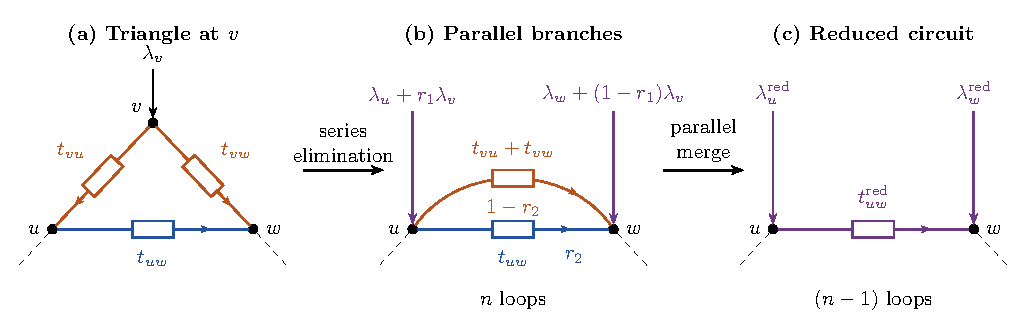
\includegraphics[width=0.78\linewidth]{figures/vec/b3-series-parallel-resistors-20261107.pdf}}\\[8pt]
\makebox[2em][l]{(b)}\raisebox{-.5\height}{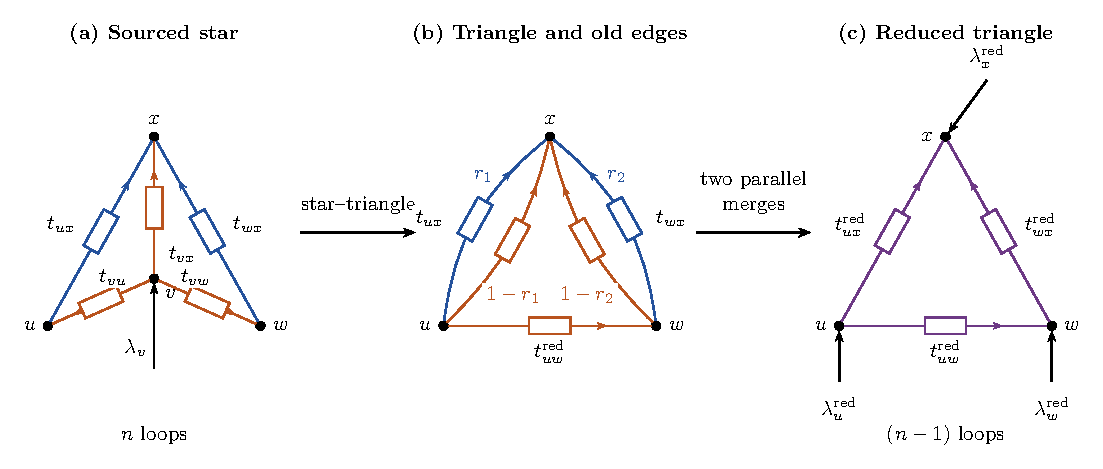
\includegraphics[width=0.78\linewidth]{figures/vec/b3-star-triangle-sourced-resistors-20261107.pdf}}\\[8pt]
\makebox[2em][l]{(c)}\raisebox{-.5\height}{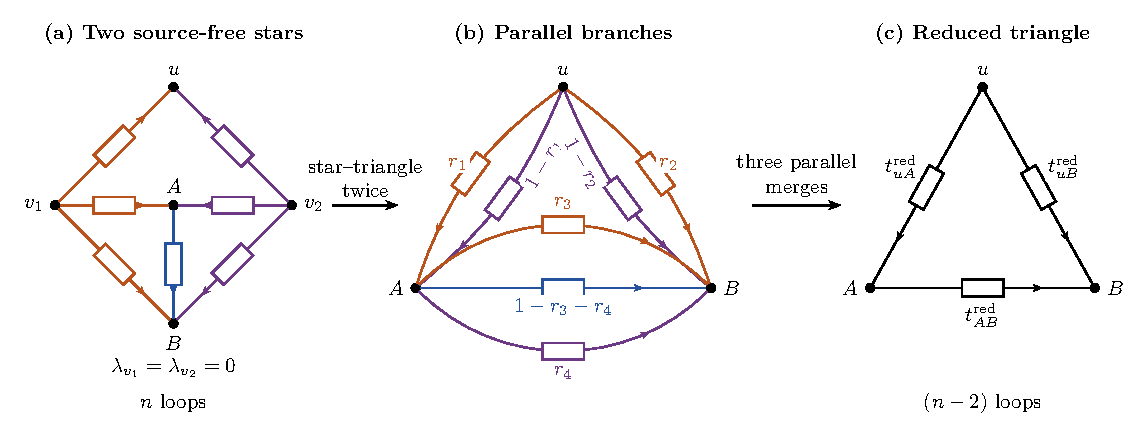
\includegraphics[width=0.78\linewidth]{figures/vec/b3-two-stars-resistors-20261107.pdf}}
\caption{The three reduction moves, derived in Sections \ref{sec-B-local-reduction} (series--parallel) and \ref{sec-forest-graphs} (star--triangle). (a) Series--parallel reduction (Theorem \ref{b-01142}): the source $\lambda_v$ is transferred to $u$ and $w$, and the series branch (orange) merges with the original $uw$ edge (blue), removing one loop. (b) Sourced star--triangle reduction (Theorem \ref{b-01159}): the source at $v$ is transferred to $u,w,x$; the blue and orange labels are fractions of the final merged currents. (c) Two source-free stars reduce to a triangle by two star--triangle moves and three parallel merges (Theorem \ref{b-01173}).}
\label{fig-sum-moves-a}
\label{fig-sum-moves-b}
\label{fig-sum-moves}
\end{figure}

The relations between the old and the new resistances, sources and currents are as follows.

\begin{tcolorbox}[enhanced,breakable,colback=white,colframe=black!45,boxrule=0.5pt,arc=1pt,left=4pt,right=4pt,top=2pt,bottom=2pt,fonttitle=\small\bfseries,title={(a) Series--parallel move (Figure \ref{fig-sum-moves}(a), Theorem \ref{b-01142}): a vertex $v$ of degree two, between $u$ and $w$}]
\begin{equation}\label{eq-sum-moves}
\begin{gathered}
r=\frac{t_{vu}}{t_{vu}+t_{vw}},\qquad t^{(1)}_{uw}=t_{vu}+t_{vw},\qquad
\lambda^{\mathrm{red}}_u=\lambda_u+(1-r)\lambda_v,\qquad
\lambda^{\mathrm{red}}_w=\lambda_w+r\lambda_v,\\
\frac1{t^{\mathrm{red}}_{uw}}=\sum_{\substack{j\\\text{parallel resistors}}}\frac1{t^{(j)}_{uw}},\qquad r_j=\frac{t^{\mathrm{red}}_{uw}}{t^{(j)}_{uw}},\qquad\sum_{\substack{j\\\text{parallel resistors}}}r_j=1,\\
y_{vu}=(1-r)\lambda_v-y^{(1)}_{uw},\qquad
y_{vw}=r\lambda_v+y^{(1)}_{uw},\qquad
y^{(j)}_{uw}=r_jy^{\mathrm{red}}_{uw}.
\end{gathered}
\end{equation}
The series step \eqref{eq-1-64} replaces the branch $u$--$v$--$w$ by one resistor and divides the source $\lambda_v$ between $u$ and $w$ in the ratio $1-r:r$; the parallel merge \eqref{eq-1-63} joins the new resistor $t^{(1)}_{uw}$ to the resistor already present between $u$ and $w$, and the current divides between them in the ratio $r_1:r_2$.
\end{tcolorbox}

\begin{tcolorbox}[enhanced,breakable,colback=white,colframe=black!45,boxrule=0.5pt,arc=1pt,left=4pt,right=4pt,top=2pt,bottom=2pt,fonttitle=\small\bfseries,title={(b) Star--triangle move (Figure \ref{fig-sum-moves}(b), Theorem \ref{b-01159}): a vertex $v$ of degree three, with neighbours $u,w,x$}]
\begin{equation}\label{eq-sum-star-triangle}
\begin{gathered}
t_{uw}^{\mathrm{red}}=t_{vu}+t_{vw}+\frac{t_{vu}t_{vw}}{t_{vx}},\qquad
\frac1{t_{ux}^{\mathrm{red}}}=\frac1{t_{ux}}+\frac{t_{vw}}{\Sigma},\qquad
\frac1{t_{wx}^{\mathrm{red}}}=\frac1{t_{wx}}+\frac{t_{vu}}{\Sigma},\\
\Sigma=t_{vu}t_{vw}+t_{vw}t_{vx}+t_{vx}t_{vu},\qquad
r_1=\frac{t_{ux}^{\mathrm{red}}}{t_{ux}},\qquad
r_2=\frac{t_{wx}^{\mathrm{red}}}{t_{wx}},\\
y_{vu}=-y_{uw}^{\mathrm{red}}-(1-r_1)y_{ux}^{\mathrm{red}},\qquad
y_{vw}=y_{uw}^{\mathrm{red}}-(1-r_2)y_{wx}^{\mathrm{red}},\\
y_{vx}=(1-r_1)y_{ux}^{\mathrm{red}}+(1-r_2)y_{wx}^{\mathrm{red}},\qquad
y_{ux}=r_1y_{ux}^{\mathrm{red}},\qquad y_{wx}=r_2y_{wx}^{\mathrm{red}}.
\end{gathered}
\end{equation}
The star at $v$ becomes a triangle on $u,w,x$, and its two new resistors merge in parallel with the resistors $t_{ux}$, $t_{wx}$ already present; $r_1$ and $r_2$ are the fractions of the merged currents carried by the old resistors. The currents are written for $\lambda_v=0$ \eqref{b-01166}; a source at $v$ is divided between $u$, $w$ and $x$ \eqref{local-B-sourced-operator}. The simultaneous removal of two source-free stars, Figure \ref{fig-sum-moves}(c), has four such fractions (Theorem \ref{b-01173}).
\end{tcolorbox}

The move (a) is the step of the recursion that Gui, Wang and Williams found, from the algebraic properties of the propagator, for the Laman graphs of type~I$'$ \cite[Theorem 4.13]{GWW}. They left the relation of their new coordinates to the Schwinger parameters open \cite[Remark 4.14]{GWW}. Here the two coordinates of each step are current-division ratios: $r$ divides the source at the eliminated vertex between its two branches, and $r_j$ divides the current between parallel resistors; their relation to the original resistances is the one in the box (a).

\section{Review of holomorphic twist}\label{sec-BV}

This section reviews the holomorphic twist of the physical theory \cite{semichiral,BK} and the graph operations of the twisted theory \cite{Costello,Wang,operatope,higher}, for readers who have not met them. It ends with the current integral \eqref{eq-C-current-delta-integral}, the starting point of our computations.

The starting point is the BV formulation of the physical theory, in which the fields, the ghosts and their antifields carry the differential $(S_{\mathrm{BV}},\,\cdot\,)$. Without the supercharge, its cohomology on local operators consists of the gauge-invariant operators modulo the equations of motion. Including one supercharge $Q_-$ in $S_{\mathrm{BV}}$ gives a complex whose cohomology consists of these operators annihilated by $Q_-$ modulo $Q_-$-exact ones, that is, the BPS sector \eqref{eq-twist-cohomology}.

The twist simplifies this complex in three steps. First, a canonical change of BV variables removes the $Q_-$-exact part of the action and exhibits most fields as pairs $(u,v)$ with $(S_{\mathrm{BV}},u)\propto v$; such pairs do not contribute to the cohomology and are dropped. What remains is the action $S_{\mathrm{tw}}$ of the holomorphic twist (Section \ref{canonical-changes-of-variables}). Second, the remaining fields and antifields assemble into four Dolbeault forms $\mathsf c,\mathsf b,\gamma,\beta$ on $\mathbb C^2$, in terms of which $S_{\mathrm{tw}}$ is a first-order action with a polynomial interaction (Section \ref{the-retained-fields}); their zero-form components are the familiar BPS letters (Section \ref{bv-completion-of-the-changyin-letters}). Third, the cohomology of the free differential $\bar\partial$ is easy to describe: it consists of the polynomials in the zero-form fields and their holomorphic derivatives (Section \ref{dolbeault-contraction-and-wick-derivatives}). The interaction then acts on these operators through the higher brackets \cite{higher,semichiral,BK} (Sections \ref{sec-brackets} and \ref{sec-brackets-origin}), which are evaluated by the current integral \cite{Wang,operatope} of Section \ref{positive-schwinger-times-and-the-operatope}.

\subsection{Coordinates and fields}\label{sec-A-conventions}

The index $A$ labels the Lie algebra and $i$ the matter representation. With the continuation $x^0=i x_E^0$, we use Euclidean spinor coordinates and the correspondingly continued sigma matrices
\begin{equation}\label{eq-Euclidean-coordinates}
x^{a\dot a}
=x_E^\mu\bar\sigma_\mu^{\dot a a}.
\end{equation}

The coordinates $x^{+\dot a}$ are holomorphic and $x^{-\dot a}$ antiholomorphic. In these coordinates,
\begin{equation}\label{eq-coordinates}
\begin{gathered}
\frac{\partial}{\partial x^{a\dot a}}=-\frac12\partial_{a\dot a},
\qquad \epsilon^{\dot+\dot-}=1=-\epsilon_{\dot+\dot-},
\qquad dx^-_{\dot a}=\epsilon_{\dot a\dot b}dx^{-\dot b},\\
\bar\partial=dx^{-\dot a}\frac{\partial}{\partial x^{-\dot a}}
=-\frac12dx^{-\dot a}\partial_{-\dot a},
\qquad\Omega=2\,dx^{+\dot+}\wedge dx^{+\dot-}.
\end{gathered}
\end{equation}

Let $c^A$ be the gauge ghost, $V^A$ the gauge field, $\lambda^A,\bar\lambda^A$ the gauginos, and $D^A$ the gauge auxiliary field. A chiral matter multiplet has components $\phi^i,\psi^i,\mathcal F^i$, with $\mathcal F^i$ the auxiliary field.
\begin{equation}\label{b-00894}
\begin{aligned}
[t_B,t_C]&=iC^A{}_{BC}t_A,\qquad
C_{ABC}=\delta_{AD}C^D{}_{BC}=C_{[ABC]},\\
f_{\mu\nu}^A&=\partial_\mu V_\nu^A-\partial_\nu V_\mu^A
+gC^A{}_{BC}V_\mu^BV_\nu^C,\\
f_{++}^A&=\partial_{+\dot a}V_+^{A\dot a}
+\frac g2C^A{}_{BC}V_{+\dot a}^BV_+^{C\dot a}.
\end{aligned}
\end{equation}

Here $\partial_\mu=\partial/\partial x_E^\mu$ and $\partial_{a\dot a}=\sigma^\mu_{a\dot a}\partial_\mu$; undotted indices use $\epsilon^{+-}=1=-\epsilon_{+-}$. Write $\bar W_{\dot a}^A(x,\theta,\bar\theta)$ for the antichiral field-strength superfield, with $\theta^a,\bar\theta^{\dot a}$ the odd superspace coordinates \cite[Eqs.~(27.2.12), (27.3.16)]{Weinberg}. Formula~\eqref{eq-field-form-dictionary} follows from the identification~$dx^{-\dot a}=4\bar\theta^{\dot a}$ in \eqref{eq-B-7}.

\subsection{Canonical changes of variables and the twisted action}\label{canonical-changes-of-variables}

In this subsection, we start from the original physical action and perform a canonical transformation (``adding $Q$-exact terms to the action''). The goal is the action $S_{\mathrm{tw}}$ of the holomorphic twist in \eqref{eq-B-5}, together with the statement \eqref{eq-twist-cohomology} that the cohomology of $(S_{\mathrm{tw}},\,\cdot\,)$ on local operators is the $Q_-$-cohomology of the physical theory.

We use the $N=1$ off-shell superfield formulation in the gauge vector representation \cite[Chapters 26--27]{Weinberg}.

Write $\Phi^{\mathcal A}$ for fields and gauge ghosts, $\Phi^\ddagger_{\mathcal A}$ for antifields, and $s$ for the gauge BRST differential; the index $\mathcal A$ runs over all component fields and ghosts, with their Lorentz, gauge and flavour indices. The BV bracket is
\begin{equation}\label{eq-A-8}
(F,G)=\int d^4x\left[
\frac{\delta_RF}{\delta\Phi^\ddagger_{\mathcal A}}
\frac{\delta_LG}{\delta\Phi^{\mathcal A}}
-\frac{\delta_RF}{\delta\Phi^{\mathcal A}}
\frac{\delta_LG}{\delta\Phi^\ddagger_{\mathcal A}}\right].
\end{equation}

Let $K$~be the K\"ahler potential and $W(\Phi,W_a)$ the chiral superpotential including its gauge kinetic term, with $W_a$ the chiral field-strength superfield. The derivatives $\nabla_a,\bar\nabla_{\dot a}$ are gauge-covariant superspace derivatives, and a vertical bar evaluates at $\theta=\bar\theta=0$, taking the lowest component. Define the odd functional
\begin{equation}\label{eq-Psi}
\Psi=\int d^4x\left[\frac18\nabla_+\bar\nabla^2K(\bar\Phi,\Phi)
+\frac12\nabla_+W(\Phi,W_a)\right]\Big|_{\theta=\bar\theta=0},
\end{equation}
which will serve as a gauge-fixing fermion. For the chosen nilpotent supercharge $Q_-$, the physical action is $Q_-\Psi$ up to the antichiral superpotential:
\begin{equation*}
\begin{aligned}
S_{\mathrm{phys}}
&=\int d^4x\,\Bigl[
\frac18\nabla_-\nabla_+\bar\nabla^2K(\bar\Phi,\Phi)
+\frac12\nabla_-\nabla_+W(\Phi,W_a)\\
&\hspace{7em}+\frac14\bar\nabla^2\bar W(\bar\Phi,\bar W_{\dot a})
\Bigr]\Big|_{\theta=\bar\theta=0},\\[6pt]
Q_-\Psi
&=\int d^4x\,\nabla_-\!\left[
\frac18\nabla_+\bar\nabla^2K(\bar\Phi,\Phi)
+\frac12\nabla_+W(\Phi,W_a)
\right]\Big|_{\theta=\bar\theta=0}\\
&=S_{\mathrm{phys}}-\frac14\int d^4x\,
\bar\nabla^2\bar W(\bar\Phi,\bar W_{\dot a})\Big|_{\theta=\bar\theta=0}.
\end{aligned}
\end{equation*}

With $S_{\mathrm{free}}$ the free quadratic kinetic action and $[\bar W]_{\bar{\mathcal F}}=\tfrac14\bar\nabla^2\bar W|_{\theta=\bar\theta=0}$ the antichiral top component, the physical and BV actions therefore have the decomposition
\begin{equation}\label{eq-B-1}
\begin{aligned}
S_{\mathrm{phys}}
&=Q_-\Psi+\int d^4x\,[\bar W(\bar\Phi,\bar W_{\dot a})]_{\bar{\mathcal F}},\\
S_{\mathrm{BV}}
&=S_{\mathrm{phys}}+\int d^4x\,((s+Q_-)\Phi^{\mathcal A})\Phi_{\mathcal A}^{\ddagger},\\
Q_{\mathrm{BV}}&=(S_{\mathrm{free}},\,\cdot),\qquad
{s\Psi=0,\quad(s+Q_-)^2=0}.
\end{aligned}
\end{equation}

We now perform the BV canonical transformation generated by the gauge-fixing fermion $\Psi$.
\begin{equation}\label{eq-B-2}
\begin{aligned}
\Phi_{\mathcal A,\mathrm{new}}^{\ddagger}
&=\Phi_{\mathcal A,\mathrm{old}}^{\ddagger}
+\frac{\delta_L\Psi}{\delta\Phi^{\mathcal A}},\qquad \Phi^{\mathcal A}_{\mathrm{new}}=\Phi^{\mathcal A}_{\mathrm{old}}\\
S_{\mathrm{BV,new}}
&=S_{\mathrm{BV,old}}\left(\Phi,
\Phi_{\mathrm{new}}^{\ddagger}-\frac{\delta_L\Psi}{\delta\Phi}\right)\\
&=\int d^4x\left([
\bar W(\bar\Phi,\bar W_{\dot a})]_{\bar{\mathcal F}}
+((s+Q_-)\Phi^{\mathcal A})\Phi_{\mathcal A,\mathrm{new}}^{\ddagger}\right).
\end{aligned}
\end{equation}

This removes the $Q_-$-exact term from the action, which cancels almost all terms in the physical action, leaving only the antichiral superpotential.

Many of the fields can be arranged into the pairs $(u,v)$ of Table~\ref{b-00904}, with $(S_{\mathrm{BV}},u)=av$ for a nonzero constant $a$. Such a pair is contractible: together with its antifields it forms a subcomplex with vanishing cohomology, so it does not contribute to the cohomology of $(S_{\mathrm{BV}},\,\cdot\,)$ and can be dropped; the precise statement is \eqref{eq-T-representative}.

{\small\renewcommand{\arraystretch}{1.25}\setlength{\tabcolsep}{4pt}
\begin{xltabular}{\linewidth}{@{}l>{\raggedright\arraybackslash}Xl@{}}
\caption{Contractible pairs of the BV complex.}\label{b-00904}\\
\toprule
$u$ & $v$ & $(S_{\mathrm{BV}},u)=av$\\
\midrule\endhead
$V_{+\dot a}^A$ & $\bar\lambda_{\dot a}^{\prime A} =\bar\lambda_{\dot a}^A-\tfrac12\nabla_{+\dot a}c^A$ & $a=-2$\\
$\lambda_+^A$ & $D^{\prime A} =D^A+gC^A{}_{BC}c^B\lambda_+^C-if_{+-}^A$ & $a=-1$\\
$\phi^i$ & $\psi_-^{\prime i} =\psi_-^i-\tfrac g{\sqrt2}c^A(t_A)^i{}_j\phi^j$ & $a=-i\sqrt2$\\
$\psi_+^i$ & $\mathcal F^{\prime i} =\mathcal F^i+\tfrac g{\sqrt2}c^A(t_A)^i{}_j\psi_+^j$ & $a=i\sqrt2$\\
\bottomrule
\end{xltabular}}

Nilpotency gives $(S_{\mathrm{BV}},v)=0$.

We perform an upper-triangular coordinate change, with $\bar\lambda\to \bar\lambda', D \to D', \psi_- \to\psi_-', \mathcal F \to\mathcal F'$; its Jacobian is one.

Let $\mathcal T$ contain these pairs and their spacetime derivatives. The remaining fields $\mathcal S=\{c,V_-,\lambda_-;\bar\phi,\bar\psi,\bar{\mathcal F}\}$ are unchanged.

The key point is that the $\mathcal S$ letters transform only among themselves (without $\mathcal T$ dependence), and the $\mathcal T$ letters form contractible pairs.

\begin{proofbox}
We remind the reader that we will contract $\mathcal T$ and keep the $\mathcal S$ letters and their antifields; however, the $\mathcal S$ letters are not the familiar ``BPS letters'', which are $\{\bar\phi_i,\ \psi_+^i,\ f_{++}^A,\ \bar\lambda_{\dot a}^A\}$ and their covariant derivatives $\nabla_{+\dot a}$ \cite{ChangYin}. The dictionary between the two sets of letters is \eqref{eq-B-14}.
\end{proofbox}

The contracting homotopy $h_{\mathcal T}$ of these pairs acts on field functionals by
\begin{equation}\label{eq-B-4}
\begin{aligned}
h_{\mathcal T}\mathcal O
&=\int_0^1\frac{dt}{t}
\left.\left(\sum_{(u,v)}\frac ua\frac{\partial_L\mathcal O}{\partial v}\right)
\right|_{(u,v)\mapsto(tu,tv)},\\
\Psi'&=h_{\mathcal T}\int d^4x\,[\bar W(\bar\Phi,\bar W_{\dot a})]_{\bar{\mathcal F}},\\
(s+Q_-)\Psi'
&=\int d^4x\,[\bar W]_{\bar{\mathcal F}}
-\left.\int d^4x\,[\bar W]_{\bar{\mathcal F}}\right|_{\mathcal T=0}.
\end{aligned}
\end{equation}

The sum includes all spacetime derivatives of each pair. The second antifield translation, generated by $\Psi'$ with the sign in \eqref{eq-B-2}, removes the $\mathcal T$ dependence of the antichiral action. It gives
\begin{equation}\label{eq-B-5}
\begin{gathered}
S_{\mathrm{BV,new}}=S_{\mathrm{tw}}+S_{\mathcal T},\qquad
S_{\mathcal T}=\int d^4x\sum_{(u,v)}av\,u^\ddagger,\\
(S_{\mathrm{tw}},S_{\mathcal T})=0,\qquad
(S_{\mathrm{tw}},S_{\mathrm{tw}})=(S_{\mathcal T},S_{\mathcal T})=0.
\end{gathered}
\end{equation}

Here $S_{\mathrm{tw}}$ depends only on the retained fields $\mathcal S$ and their antifields: it is the action of the holomorphic twist, written out in \eqref{eq-B-8}, and $S_{\mathcal T}$ is the quadratic action of the contractible pairs.

\begin{proofbox}
Including the antifields and all spacetime derivatives of the pairs, the contracting homotopy satisfies
\begin{equation}\label{eq-B-6}
\begin{aligned}
(S_{\mathrm{BV}},v^\ddagger)&=(-1)^{|u|}a u^\ddagger,
&(S_{\mathrm{BV}},u^\ddagger)&=0,\\
h_{\mathcal T}\mathcal O
&=\int_0^1\frac{dt}{t}\left.
\sum_{(u,v)}\left(\frac ua\frac{\partial_L}{\partial v}
+\frac{(-1)^{|u|}v^\ddagger}{a}
\frac{\partial_L}{\partial u^\ddagger}\right)\mathcal O
\right|_{\mathcal T\mapsto t\mathcal T},\\
(S_{\mathrm{BV}},h_{\mathcal T}\mathcal O)
+h_{\mathcal T}(S_{\mathrm{BV}},\mathcal O)
&=\mathcal O-\mathcal O|_{\mathcal T=0},\qquad [h_{\mathcal T},\partial_\mu]=0.
\end{aligned}
\end{equation}

For $(S_{\mathrm{BV}},\mathcal O)=0$, this gives
\begin{equation}\label{eq-T-representative}
\mathcal O=\mathcal O|_{\mathcal T=0}
+(S_{\mathrm{BV}},h_{\mathcal T}\mathcal O).
\end{equation}

The representative on the right contains only retained fields and antifields in the complex $\mathcal S$.
\end{proofbox}

In particular,
\begin{equation}\label{eq-T-projection}
\nabla_{+\dot a}\longmapsto\partial_{+\dot a},\qquad
\bar\lambda_{\dot a}^A\longmapsto
\frac12\partial_{+\dot a}c^A
=-\frac{\partial c^A}{\partial x^{+\dot a}}.
\end{equation}

The complex of $S_{\mathrm{tw}}$ computes the BPS operators of the physical theory. On local operators that do not contain the undifferentiated ghost $c^A$,
\begin{equation}\label{eq-twist-cohomology}
H\bigl((S_{\mathrm{tw}},\,\cdot\,)\bigr)
\;\cong\;H\bigl((S_{\mathrm{BV}},\,\cdot\,)\bigr)
\;\cong\;H\Bigl(Q_-\,;\ \frac{\text{gauge-invariant local operators}}{\text{equations of motion}}\Bigr).
\end{equation}
The first isomorphism follows from \eqref{eq-T-representative}. The second says that the cohomology of the total differential, which contains the gauge BRST transformation, the equations of motion and $Q_-$, is the cohomology of $Q_-$ on the BRST cohomology of the physical theory, that is, on the gauge-invariant local operators modulo the equations of motion. This identification is widely accepted, and earlier work on twisted theories uses it without comment \cite{CostelloTwist,SaberiWilliams,ESW,semichiral,BK}. Appendix \ref{app-twist-cohomology} gives a proof (Proposition \ref{prop-twist-cohomology}) and its form in perturbation theory (Proposition \ref{prop-twist-cohomology-quantum}).

\subsection{The retained fields as Dolbeault forms}\label{the-retained-fields}

In the remaining complex $\mathcal S$, the fields and antifields assemble into four superfields in the odd coordinate $\bar\theta^{\dot a}$, that is, into differential forms in $dx^{-\dot a}$ (Dolbeault forms):
\begin{equation}\label{eq-B-7}
\begin{aligned}
\mathsf c^A&=c^A-2\bar\theta_{\dot a}V_-^{A\dot a}
+2i\bar\theta_{\dot a}\bar\theta^{\dot a}\lambda_-^A,\\
\gamma_i&=\bar\phi_i-\sqrt2\bar\theta_{\dot a}\bar\psi_i^{\dot a}
+\bar\theta_{\dot a}\bar\theta^{\dot a}\bar{\mathcal F}_i,\\
\beta^i&=\bar{\mathcal F}^{\ddagger i}
+\sqrt2\bar\theta_{\dot a}\bar\psi^{\ddagger\dot ai}
+\bar\theta_{\dot a}\bar\theta^{\dot a}\bar\phi^{\ddagger i},\\
\mathsf b_A&=-\frac i2\lambda_A^{\ddagger-}
+\bar\theta_{\dot a}V_A^{\ddagger-\dot a}
+\bar\theta_{\dot a}\bar\theta^{\dot a}c_A^{\ddagger},\\
\bar\partial&=2\bar\theta_{\dot a}\partial_-{}^{\dot a},
\qquad dx^{-\dot a}=4\bar\theta^{\dot a}.
\end{aligned}
\end{equation}

\begin{proofbox}
Here $\bar\psi^\ddagger_{\dot a}{}^i$ is BV-dual to $\bar\psi_i^{\dot a}$, and $\bar\psi^{\ddagger\dot a i}$ in $\beta^i$ has its dotted index raised as in \eqref{eq-coordinates}.
\begin{equation*}
\begin{aligned}
\bar\psi^\ddagger_{\dot a}{}^i
\bigl((s+Q_-)\bar\psi_i^{\dot a}\bigr)
&=-\bigl((s+Q_-)\bar\psi_{i\dot a}\bigr)
\bar\psi^{\ddagger\dot a i},\\
\sqrt2\bar\theta_{\dot a}\bar\psi^{\ddagger\dot a i}
&=-\sqrt2\bar\psi^\ddagger_{\dot a}{}^i\bar\theta^{\dot a}.
\end{aligned}
\end{equation*}
\end{proofbox}

The last line is \eqref{eq-coordinates} in these variables: with $dx^{-\dot a}=4\bar\theta^{\dot a}$, $\bar\partial=-\frac12dx^{-\dot a}\partial_{-\dot a}=-2\bar\theta^{\dot a}\partial_{-\dot a}=2\bar\theta_{\dot a}\partial_-{}^{\dot a}$. The components are arranged so that the BV differential of the free theory acts on the four forms as $\bar\partial$; for example, with the differential anticommuting with $\bar\theta$, the gauge variation $sV_-^{A\dot a}=\partial_-{}^{\dot a}c^A+\ldots$ gives $(S_{\mathrm{BV}},-2\bar\theta_{\dot a}V_-^{A\dot a})=2\bar\theta_{\dot a}\partial_-{}^{\dot a}c^A+\ldots$, the one-form part of $\bar\partial\mathsf c^A$.

The identification $dx^{-\dot a}=4\bar\theta^{\dot a}$ and the volume relation
\begin{equation}\label{b-00919}
\Omega\wedge dx^{-\dot+}\wedge dx^{-\dot-}=-8\,d^4x_E,
\qquad d^4x_E=dx_E^0\wedge dx_E^1\wedge dx_E^2\wedge dx_E^3
\end{equation}
turn $S_{\mathrm{tw}}$ of \eqref{eq-B-5} into an integral over $\mathbb C^2$:

\rthm{Proposition}{b-00164}{Twisted action and interaction density \cite{semichiral,BK}} With $(t_A)^j{}_i$ the generators in the matter representation, the action of the holomorphic twist is
\begin{equation}\label{eq-B-8}
\begin{aligned}
S_{\mathrm{tw}}=\int_{\mathbb C^2}\Omega\wedge\Big[
&\mathsf b_A\left(\bar\partial\mathsf c^A
-\frac g2C^A{}_{BC}\mathsf c^B\mathsf c^C\right)\\
&+\left(\bar\partial\gamma_i-ig\mathsf c^A(t_A)^j{}_i\gamma_j\right)\beta^i
+\bar W(\gamma,\mathsf w)\Big]_{(0,2)}.
\end{aligned}
\end{equation}
where the projection $[\cdot]_{(0,2)}$ selects antiholomorphic form degree two and the function $\bar W$ contains the antichiral superpotential and gauge kinetic terms expressed in $\gamma$ and $\mathsf w$. $\Omega$ is the holomorphic form $2\,dx^{+\dot+}\wedge dx^{+\dot-}$.

In the main text, $\bar W$ is a polynomial or, more generally, a formal power series in $\gamma$ and $\mathsf w$, read coefficientwise, as perturbation theory requires. Appendix~\ref{app-covariant-derivatives} treats superpotentials containing covariant derivatives.

The interaction density entering the higher operations is~
\begin{equation}\label{eq-B-10}
\mathcal I=-\frac g2C^A{}_{BC}\mathsf b_A\mathsf c^B\mathsf c^C
-ig\mathsf c^A(t_A)^j{}_i\gamma_j\beta^i
+\bar W(\gamma,\mathsf w).
\end{equation}

\begin{proofbox}
$\mathcal I$ in \eqref{eq-B-10} is a polynomial in the full Dolbeault fields, retaining all antiholomorphic form degrees.

Its integrated interaction is $I=\int_{\mathbb C^2}\Omega\wedge[\mathcal I]_{(0,2)}$.

In \eqref{eq-A-28}, Wick contraction precedes the final $H(\bar\partial)$ projection: only the surviving fields are replaced by their holomorphic zero-form Taylor expansions.

The propagator forms remain in the integral and supply its antiholomorphic integration degree.
\end{proofbox}

Its free kinetic part is
\begin{equation}\label{eq-BV-free-action}
\begin{aligned}
S_{\mathrm{free}}&=\int_{\mathbb C^2}\Omega\wedge
[\mathsf b_A\bar\partial\mathsf c^A+(\bar\partial\gamma_i)\beta^i]_{(0,2)},\\
Q_{\mathrm{BV}}&=(S_{\mathrm{free}},\cdot)=\bar\partial,
\qquad (S_{\mathrm{tw}},\cdot)=Q_{\mathrm{BV}}+(I,\cdot).
\end{aligned}
\end{equation}

A superscript $(0)$ denotes the zero-form component of a Dolbeault form. In terms of the original antifields, before the two antifield translations \eqref{eq-B-2} generated by $\Psi$ and $\Psi'$, the zero-form components of $\beta$ and $\mathsf b$ are
\begin{equation}\label{eq-B-11}
\begin{aligned}
\beta^{(0)i}
&=\bar{\mathcal F}_{\mathrm{old}}^{\ddagger i}
+\frac{\delta_L(\Psi+\Psi')}{\delta\bar{\mathcal F}_i},\\
\mathsf b_A^{(0)}
&=-\frac i2\left(
\lambda_{A,\mathrm{old}}^{\ddagger-}
+\frac{\delta_L(\Psi+\Psi')}{\delta\lambda_-^A}\right).
\end{aligned}
\end{equation}

For canonical matter and quadratic gauge kinetic terms, the combined translation has generator
\begin{equation}\label{eq-B-12}
\begin{aligned}
\Psi+\Psi'=\int d^4x\,\Big[
&-\frac1{\sqrt2}\phi^i\nabla_{+\dot a}\bar\psi_i^{\dot a}
+g\bar\phi_j(t_A)^j{}_i\phi^i\lambda_+^A\\
&-\frac i{\sqrt2}\bar{\mathcal F}_i\psi_+^i
-\frac i{\sqrt2}\psi_+^i\frac{\partial W(\phi,0)}{\partial\phi^i}\\
&+\frac i2\delta_{AB}f_{++}^A\lambda_-^B
-\frac12\delta_{AB}(D^A+if_{+-}^A)\lambda_+^B\Big].
\end{aligned}
\end{equation}

They give
\begin{equation}\label{eq-B-13}
\begin{aligned}
\beta^{(0)i}
&=\bar{\mathcal F}_{\mathrm{old}}^{\ddagger i}
-\frac i{\sqrt2}\psi_+^i,\\
\mathsf b_A^{(0)}
&
=-\frac i2\lambda_{A,\mathrm{old}}^{\ddagger-}
+\frac14\delta_{AB}f_{++}^B.
\end{aligned}
\end{equation}

Collecting \eqref{eq-B-7} and \eqref{eq-B-13}, with $dx^{-\dot a}=4\bar\theta^{\dot a}$, gives the dictionary between the Dolbeault fields $\mathsf c^A,\mathsf b_A,\gamma_i,\beta^i$ and the physical components.\label{fields-and-interaction}

\rthm{Proposition}{b-00159}{Component dictionary} \emph{For canonical matter and quadratic gauge kinetic terms, the map between twisted theory and physical components is}
\begin{equation}\label{eq-field-form-dictionary}
\begin{aligned}
\mathsf c^A={}&c^A-\frac12dx^-_{\dot a}V_-^{A\dot a}
 +\frac i4dx^{-\dot+}\wedge dx^{-\dot-}\lambda_-^A,\\
\gamma_i={}&\bar\phi_i-\frac1{2\sqrt2}dx^-_{\dot a}\bar\psi_i^{\dot a}
 +\frac18dx^{-\dot+}\wedge dx^{-\dot-}\bar{\mathcal F}_i,\\
\beta^i={}&\bar{\mathcal F}^{\ddagger i}
 -\frac i{\sqrt2}\psi_+^i
 +\frac1{2\sqrt2}dx^-_{\dot a}\bar\psi^{\ddagger\dot a i}
 +\frac18dx^{-\dot+}\wedge dx^{-\dot-}\bar\phi^{\ddagger i},\\
\mathsf b_A={}&\frac14\delta_{AB}f_{++}^B
 -\frac i2\lambda_A^{\ddagger-}
 +\frac14dx^-_{\dot a}V_A^{\ddagger-\dot a}
 +\frac18dx^{-\dot+}\wedge dx^{-\dot-}c_A^\ddagger,\\
\mathsf w_{\dot a}^A={}&
 \left.\bar W_{\dot a}^A\right|_{\theta=0,\,
 \bar\theta^{\dot b}=dx^{-\dot b}/4}\\
={}&\bar\lambda_{\dot a}^A+\frac i4dx^-_{\dot a}D^A
 +\frac18dx^{-\dot b}\epsilon^{bc}
 \sigma^\mu_{b\dot a}\sigma^\nu_{c\dot b}f_{\mu\nu}^A\\
&-\frac i8dx^{-\dot+}\wedge dx^{-\dot-}
 \nabla^b{}_{\dot a}\lambda_b^A.
\end{aligned}
\end{equation}
\emph{where $\ddagger$ denotes the antifield.\footnote{Homotopy transfer sends the antichiral field strength to
\begin{equation}\label{footnote-16--eq3.4}
\begin{aligned}
\mathsf w_{\dot a}^A
&\xmapsto{\text{homotopy transfer}}\frac12\partial_{+\dot a}\mathsf c^A
=-\frac{\partial\mathsf c^A}{\partial x^{+\dot a}}\\
&=\frac12\partial_{+\dot a}c^A
-\frac14dx^-_{\dot b}\partial_{+\dot a}V_-^{A\dot b}
+\frac i8dx^{-\dot+}\wedge dx^{-\dot-}
 \partial_{+\dot a}\lambda_-^A.
\end{aligned}
\end{equation}
\begin{equation*}
[\bar\lambda_{\dot a}^A]
=[\mathsf w_{\dot a}^{A(0)}]
=\frac12[\partial_{+\dot a}\mathsf c^{A(0)}].
\end{equation*}
The doublet $(S_{\mathrm{BV}},V_{+\dot a}^A) =-2\bar\lambda_{\dot a}^A+\nabla_{+\dot a}c^A$ identifies the gaugino with the zero-form part of $\tfrac12\partial_{+\dot a}\mathsf c^A$ after transfer.}}

For the quadratic gauge kinetic term,
\begin{equation}\label{b-00931}
-\frac14\delta_{AB}\mathsf w_{\dot a}^A\mathsf w^{B\dot a}
=-\frac1{16}\delta_{AB}\partial_{+\dot a}
  (\mathsf c^A\partial_+{}^{\dot a}\mathsf c^B),
\end{equation}
so it is a total derivative.

\subsection{BV completion of the Chang--Yin letters}\label{bv-completion-of-the-changyin-letters}

For the canonical kinetic terms of \eqref{eq-B-12}, the BPS letters of Chang and Yin \cite[Section 2]{ChangYin} are the scalar $\bar\phi(z)$, chiral fermion $\psi_+(z)$, self-dual curvature $f_{++}(z)$ and antichiral gaugino $\bar\lambda(z)$. Their component complex uses the auxiliary $\bar{\mathcal F}$ and gaugino $\lambda^{-}$ equations of motion (which are exactly the antifield parts of $\beta$ and $\mathsf b$). In the present conventions these equations are
\begin{equation}\label{eq-CY-component-equations}
\mathcal F^i+\frac{\partial\bar W(\bar\phi,0)}{\partial\bar\phi_i}=0,
\qquad
\nabla_{+\dot a}\bar\lambda^{A\dot a}
-\sqrt2g\delta^{AB}\bar\phi_j(t_B)^j{}_i\psi_+^i=0.
\end{equation}

The original antifields implement these equations within the BV complex:
\begin{equation}\label{eq-CY-antifield-equations}
\begin{aligned}
(S_{\mathrm{BV}},\bar{\mathcal F}_{\mathrm{old}}^{\ddagger i})
&=igc^A(t_A)^i{}_j\bar{\mathcal F}_{\mathrm{old}}^{\ddagger j}
-\mathcal F^i-\frac{\partial\bar W(\bar\phi,0)}{\partial\bar\phi_i},\\
(S_{\mathrm{BV}},\lambda_{A,\mathrm{old}}^{\ddagger-})
&=-gC^B{}_{AC}c^C\lambda_{B,\mathrm{old}}^{\ddagger-}
+i\delta_{AB}\nabla_{+\dot a}\bar\lambda^{B\dot a}\\
&\quad-i\sqrt2g\bar\phi_j(t_A)^j{}_i
 \left(\psi_+^i+i\sqrt2\bar{\mathcal F}_{\mathrm{old}}^{\ddagger i}\right).
\end{aligned}
\end{equation}

The completed fermion and curvature are precisely the retained letters of \eqref{eq-B-13}, with their fixed component factors:
\begin{equation}\label{eq-CY-completed-letters}
\psi_+^i+i\sqrt2\bar{\mathcal F}_{\mathrm{old}}^{\ddagger i}
=i\sqrt2\beta^{(0)i},\qquad
f_{++}^A-2i\delta^{AB}\lambda_{B,\mathrm{old}}^{\ddagger-}
=4\delta^{AB}\mathsf b_B^{(0)}.
\end{equation}

Using $Q_-\psi_+^i=i\sqrt2\mathcal F^i$ and $Q_-f_{++}^A=-2\nabla_{+\dot a}\bar\lambda^{A\dot a}$ gives
\begin{equation}\label{eq-CY-completion-images}
\begin{aligned}
&(S_{\mathrm{BV}},
 \psi_+^i+i\sqrt2\bar{\mathcal F}_{\mathrm{old}}^{\ddagger i})\\
&\quad=igc^A(t_A)^i{}_j\left(\psi_+^j+i\sqrt2\bar{\mathcal F}_{\mathrm{old}}^{\ddagger j}\right)
-i\sqrt2\frac{\partial\bar W(\bar\phi,0)}{\partial\bar\phi_i},\\
&(S_{\mathrm{BV}},f_{++}^A-2i\delta^{AB}\lambda_{B,\mathrm{old}}^{\ddagger-})\\
&\quad=-gC^A{}_{BC}c^B\left(f_{++}^C-2i\delta^{CD}\lambda_{D,\mathrm{old}}^{\ddagger-}\right)
-2\nabla_{+\dot a}\bar\lambda^{A\dot a}\\
&\qquad-2i\left[i\nabla_{+\dot a}\bar\lambda^{A\dot a}
-i\sqrt2g\delta^{AB}\bar\phi_j(t_B)^j{}_i
 \left(\psi_+^i+i\sqrt2\bar{\mathcal F}_{\mathrm{old}}^{\ddagger i}\right)\right]\\
&\quad=-4g\delta^{AB}C^C{}_{BD}c^D\mathsf b_C^{(0)}
-4ig\delta^{AB}\bar\phi_j(t_B)^j{}_i\beta^{(0)i}.
\end{aligned}
\end{equation}

The auxiliary field and the gaugino divergence cancel, leaving the familiar classical terms and keeping the $\mathcal S$ complex closed under $(S_{\mathrm{BV}},\cdot)$.

At the insertion $x=0$, physical operators are gauge-invariant words independent of the undifferentiated ghost $c^A(0)$.

We can now build the full dictionary between the twisted letters and the Chang--Yin letters, with all their holomorphic derivatives.

The symbol $\longleftrightarrow$ denotes the image after the contraction of the pairs of Table~\ref{b-00904} and the projection to the holomorphic derivatives of the zero-form fields. Parentheses symmetrize the dotted indices with weight one, and $n\ge0$.
\begin{equation}\label{eq-B-14}
\begin{aligned}
\nabla_{+(\dot a_1}\cdots\nabla_{+\dot a_n)}\bar\phi_i
&\longleftrightarrow
\partial_{+\dot a_1}\cdots\partial_{+\dot a_n}\gamma_i^{(0)},\\
\nabla_{+(\dot a_1}\cdots\nabla_{+\dot a_n)}
\left(\psi_+^i+i\sqrt2\bar{\mathcal F}_{\mathrm{old}}^{\ddagger i}\right)
&\longleftrightarrow
 i\sqrt2\partial_{+\dot a_1}\cdots\partial_{+\dot a_n}\beta^{(0)i},\\
\nabla_{+(\dot a_1}\cdots\nabla_{+\dot a_n)}
\left(f_{++}^A-2i\delta^{AB}\lambda_{B,\mathrm{old}}^{\ddagger-}\right)
&\longleftrightarrow
 4\delta^{AB}\partial_{+\dot a_1}\cdots\partial_{+\dot a_n}\mathsf b_B^{(0)},\\
2\nabla_{+(\dot a_1}\cdots\nabla_{+\dot a_n}\bar\lambda_{\dot a_0)}^A
&\longleftrightarrow
\partial_{+\dot a_0}\cdots\partial_{+\dot a_n}\mathsf c^{A(0)}.
\end{aligned}
\end{equation}

\begin{proofbox}
Ordered covariant derivatives reduce to symmetrized derivatives and curvature terms. Completing each $f_{++}^A$ to $f_{++}^A-2i\delta^{AB}\lambda_{B,\mathrm{old}}^{\ddagger-}$ gives representatives in the retained complex.

For ordered derivatives, the curvature commutator determines the additional $\mathsf b$ term. Since $\nabla_{+\dot a}\bar\phi_i=\partial_{+\dot a}\bar\phi_i +igV_{+\dot a}^A(t_A)^j{}_i\bar\phi_j$, the full BV variation is
\begin{equation}\label{eq-ordered-scalar-variation}
\begin{aligned}
(S_{\mathrm{BV}},\nabla_{+\dot a}\nabla_+{}^{\dot b}\bar\phi_i)
={}&-igc^A(t_A)^j{}_i\nabla_{+\dot a}\nabla_+{}^{\dot b}\bar\phi_j\\
&-2ig\Big[
 \frac12\left(\nabla_{+\dot a}\bar\lambda^{A\dot b}
 +\nabla_+{}^{\dot b}\bar\lambda_{\dot a}^A\right)\bar\phi_j
 +\bar\lambda_{\dot a}^A\nabla_+{}^{\dot b}\bar\phi_j
 +\bar\lambda^{A\dot b}\nabla_{+\dot a}\bar\phi_j
 \Big](t_A)^j{}_i\\
&-ig\delta_{\dot a}{}^{\dot b}
 (\nabla_{+\dot c}\bar\lambda^{A\dot c})
 (t_A)^j{}_i\bar\phi_j.
\end{aligned}
\end{equation}

The last term has the free gaugino equation as its linear field factor. The complementary antifield term has variation
\begin{equation}\label{eq-ordered-scalar-complement}
\begin{aligned}
&\left(S_{\mathrm{BV}},
g\delta_{\dot a}{}^{\dot b}\delta^{AB}\lambda_{B,\mathrm{old}}^{\ddagger-}
 (t_A)^j{}_i\bar\phi_j\right)
\\
&\quad=-ig^2\delta_{\dot a}{}^{\dot b}\delta^{AB}c^C
\lambda_{B,\mathrm{old}}^{\ddagger-}(t_C)^j{}_i(t_A)^k{}_j\bar\phi_k\\
&\qquad+ig\delta_{\dot a}{}^{\dot b}
 (\nabla_{+\dot c}\bar\lambda^{A\dot c})(t_A)^j{}_i\bar\phi_j\\
&\qquad-i\sqrt2g^2\delta_{\dot a}{}^{\dot b}\delta^{AB}
 \bar\phi_k(t_B)^k{}_\ell
 \left(\psi_+^\ell+i\sqrt2\bar{\mathcal F}_{\mathrm{old}}^{\ddagger\ell}\right)
 (t_A)^j{}_i\bar\phi_j.
\end{aligned}
\end{equation}

The divergence cancels between these two equations.
\begin{equation}\label{eq-B-16}
\begin{aligned}
&\nabla_{+\dot a}\nabla_+{}^{\dot b}\bar\phi_i
+g\delta_{\dot a}{}^{\dot b}\delta^{AB}\lambda_{B,\mathrm{old}}^{\ddagger-}
 (t_A)^j{}_i\bar\phi_j\\
&\quad=\frac12\left(\nabla_{+\dot a}\nabla_+{}^{\dot b}
+\nabla_+{}^{\dot b}\nabla_{+\dot a}\right)\bar\phi_i
+\frac{ig}{2}\delta_{\dot a}{}^{\dot b}
 \left(f_{++}^A-2i\delta^{AB}\lambda_{B,\mathrm{old}}^{\ddagger-}\right)
 (t_A)^j{}_i\bar\phi_j\\
&\quad\longleftrightarrow
\partial_{+\dot a}\partial_+{}^{\dot b}\gamma_i^{(0)}
+2ig\delta_{\dot a}{}^{\dot b}\delta^{AB}\mathsf b_B^{(0)}
 (t_A)^j{}_i\gamma_j^{(0)}.
\end{aligned}
\end{equation}

The antisymmetric derivative of the gaugino gives the other relation used in \cite[Eq.~(2.4)]{ChangYin}. Equation~\eqref{eq-CY-antifield-equations} gives the explicit BV boundary
\begin{equation}\label{eq-B-17}
\begin{aligned}
&\nabla_{+\dot a}\bar\lambda^{A\dot b}
+\frac{ig}{2}\delta_{\dot a}{}^{\dot b}\delta^{AB}
 C^C{}_{BD}c^D\lambda_{C,\mathrm{old}}^{\ddagger-}\\
&\quad-\left[\frac12\left(\nabla_{+\dot a}\bar\lambda^{A\dot b}
+\nabla_+{}^{\dot b}\bar\lambda_{\dot a}^A\right)
+\frac g{\sqrt2}\delta_{\dot a}{}^{\dot b}\delta^{AB}
 \bar\phi_j(t_B)^j{}_i
 \left(\psi_+^i+i\sqrt2\bar{\mathcal F}_{\mathrm{old}}^{\ddagger i}\right)\right]\\
&\qquad=\left(S_{\mathrm{BV}},
 -\frac i2\delta_{\dot a}{}^{\dot b}\delta^{AB}\lambda_{B,\mathrm{old}}^{\ddagger-}\right).
\end{aligned}
\end{equation}

The representative in square brackets transfers as
\begin{equation}\label{eq-CY-gaugino-transferred}
\begin{aligned}
&\frac12\left(\nabla_{+\dot a}\bar\lambda^{A\dot b}
+\nabla_+{}^{\dot b}\bar\lambda_{\dot a}^A\right)
+\frac g{\sqrt2}\delta_{\dot a}{}^{\dot b}\delta^{AB}
\bar\phi_j(t_B)^j{}_i
\left(\psi_+^i+i\sqrt2\bar{\mathcal F}_{\mathrm{old}}^{\ddagger i}\right)\\
&\qquad\longleftrightarrow
\frac12\partial_{+\dot a}\partial_+{}^{\dot b}\mathsf c^{A(0)}
+ig\delta_{\dot a}{}^{\dot b}\delta^{AB}(t_B)^j{}_i
\gamma_j^{(0)}\beta^{(0)i}.
\end{aligned}
\end{equation}
\end{proofbox}

The induced classical differential acts on the four zero-form fields by
\begin{equation}\label{eq-B-15}
\begin{aligned}
Q_0\mathsf c^A&=-\frac g2 C^A{}_{BC}\mathsf c^B\mathsf c^C,
&Q_0\gamma_i&=-ig\mathsf c^A(t_A)^j{}_i\gamma_j,\\
Q_0\beta^i&=ig\mathsf c^A(t_A)^i{}_j\beta^j
-\frac{\partial\bar W(\gamma,0)}{\partial\gamma_i},
&Q_0\mathsf b_A&=-gC^B{}_{AC}\mathsf c^C\mathsf b_B
-ig(t_A)^j{}_i\gamma_j\beta^i.
\end{aligned}
\end{equation}

Here all fields denote their zero-form parts, and $[Q_0,\partial_{+\dot a}]=0$ supplies the transformations of all their holomorphic derivatives.

\subsection{Holomorphic local operators}\label{dolbeault-contraction-and-wick-derivatives}

The free part of $(S_{\mathrm{tw}},\,\cdot\,)$ is $\bar\partial$ \eqref{eq-BV-free-action}. We now prove that, with the twisted action $S_{\mathrm{tw}}$, the antiholomorphic parts of the letters are indeed contractible: the cohomology of $\bar\partial$ on local operators consists of the polynomials in the zero-form fields and their holomorphic derivatives.

We use the perturbative homotopy transfer of Section \ref{sec-homotopy-transfer}, one step before its page $E_0$: we first take the $\bar\partial$-cohomology of the letters.

The letters of a local operator are the Taylor coefficients of the Dolbeault fields at the insertion point, so we work with polynomial differential forms in $x^{\pm\dot a}$ and $dx^{-\dot a}$. Let $\iota$ include the holomorphic representatives and $\pi$ project onto them.~ Here $\iota_{-\dot a}$ contracts a differential form with $\partial/\partial x^{-\dot a}$; $N$ counts antiholomorphic coordinate and form degree:
\begin{equation}\label{eq-B-20}
\begin{gathered}
\{\bar\partial,\iota_{-\dot a}\}=\frac{\partial}{\partial x^{-\dot a}},
\qquad
N=\{\bar\partial,\iota_{x^{-\dot a}\partial/\partial x^{-\dot a}}\}
=x^{-\dot a}\frac{\partial}{\partial x^{-\dot a}}
+dx^{-\dot a}\iota_{-\dot a},\\
\pi X=X\big|_{x^{-\dot a}=dx^{-\dot a}=0},
\qquad
h_{\bar\partial}=\begin{cases}
\iota_{x^{-\dot a}\partial/\partial x^{-\dot a}}N^{-1},&N>0,\\
0,&N=0,
\end{cases}\\
\bar\partial h_{\bar\partial}+h_{\bar\partial}\bar\partial=1-\iota\pi,
\qquad h_{\bar\partial}^2=h_{\bar\partial}\iota=\pi h_{\bar\partial}=0.
\end{gathered}
\end{equation}

Indeed, by Cartan's formula $N$ is the Lie derivative along the vector field $x^{-\dot a}\partial/\partial x^{-\dot a}$: it multiplies a monomial by its total degree in $x^{-\dot a}$ and $dx^{-\dot a}$ and commutes with $\bar\partial$, so $\bar\partial h_{\bar\partial}+h_{\bar\partial}\bar\partial=NN^{-1}=1$ on the monomials with $N>0$, and the monomials with $N=0$ are the holomorphic polynomials without $dx^{-\dot a}$. The contraction therefore removes antiholomorphic coordinates and forms, leaving the holomorphic derivatives of the zero-form fields. For a Dolbeault-closed output field, translation therefore acts as
\begin{equation}\label{eq-B-21}
\begin{aligned}
\pi X(x_v+x)
&=\pi\exp\left(x_v^{+\dot a}\frac{\partial}{\partial x^{+\dot a}}
+x_v^{-\dot a}\frac{\partial}{\partial x^{-\dot a}}\right)X(x)\\
&=\exp\left(x_v^{+\dot a}\frac{\partial}{\partial x^{+\dot a}}\right)\pi X(x).
\end{aligned}
\end{equation}

\subsection{Quantization of the twist theory and higher brackets}\label{sec-brackets}\label{sec-setup}

Quantization of the physical theory, including its regularization and renormalization, is technically demanding. As in the previous works \cite{semichiral,operatope,higher,BK}, we therefore quantize the classical twisted theory. We should warn the reader that the equivalence with twisting the quantized physical theory, in the all-orders generality needed for the theories and composite operators considered here, has not been established in any of these previous works. Known supersymmetry anomalies, including the generalized Konishi anomaly, provide evidence for this identification \cite[Section 2.2]{BK}; we assume it when interpreting the twisted cohomology as the physical quantum BPS sector. Appendix~\ref{app-twist-cohomology} explains the conditional cohomological comparison.

\paragraph{From the functional integral to the BV pairing.}

Naive perturbation theory starts from a gauge-fixed functional integral
\begin{equation}\label{eq-C-formal-integral}
\int_{\mathcal L}\mathcal O(e)\,
\exp\!\left[\frac{S_{\mathrm{free}}(e)+I(e)}{\hbar}\right]\mathcal D e,
\qquad S_{\mathrm{tw}}=S_{\mathrm{free}}+I,
\qquad I=\int_{\mathbb C^2}\Omega\wedge[\mathcal I]_{(0,2)}.
\end{equation}
Here $e$ denotes the collective Dolbeault BV fields $\mathsf c,\mathsf b,\gamma,\beta$, $E$ is their graded space, and $\mathcal L\subset E$ is the gauge-fixing Lagrangian subspace; $\mathcal D e$ denotes the formal integration measure. Costello's construction \cite{Costello,CostelloBV} replaces this expression by a regularized Wick expansion and a master equation at each scale. To construct that expansion we need the free quadratic action, its gauge-fixed inverse, and the pairing that specifies which fields can contract.

The odd, nondegenerate BV pairing $\omega_E$ pairs $\mathsf b_A$ with $\mathsf c^A$ and $\beta^i$ with $\gamma_i$, integrated with $\Omega$. Its inverse defines the antibracket \eqref{eq-A-8}. With the free BV differential $Q_{\mathrm{BV}}=\bar\partial$ of \eqref{eq-BV-free-action}, the quadratic action is
\begin{equation}\label{eq-C-quadratic-action}
\begin{aligned}
S_{\mathrm{free}}(e)
&=\frac12\omega_E(e,Q_{\mathrm{BV}}e)
=\int_{\mathbb C^2}\Omega\wedge
\bigl[\mathsf b_A\bar\partial\mathsf c^A
+(\bar\partial\gamma_i)\beta^i\bigr]_{(0,2)},\\
\delta S_{\mathrm{free}}(e)
&=\omega_E(\delta e,Q_{\mathrm{BV}}e),
\qquad (S_{\mathrm{free}},\,\cdot\,)=Q_{\mathrm{BV}}.
\end{aligned}
\end{equation}
The second line follows by graded integration by parts for compactly supported variations $\delta e$. Thus the free BV transformation is generated by the quadratic action through the antibracket: $(S_{\mathrm{free}},e)=Q_{\mathrm{BV}}e$. The factor $1/2$ counts the two paired terms once. This uses the $e^{S/\hbar}$ convention of \cite{CostelloBV}: the Gaussian contour is chosen so that the bosonic quadratic form is negative definite, rather than inserting an extra minus sign in the Wick operator.

The inverse pairing $\omega_E^{-1}$ is a spacetime delta function times a constant field-space tensor. Contracting one unordered pair of fields with it gives the formal BV Laplacian $\Delta=\partial_{\omega_E^{-1}}$. For a pair at distinct labelled vertices $v,w$, its contribution is
\begin{equation}\label{eq-pairing-Delta}
\partial_{\omega_E^{-1}}=[K_0(x_v,x_w)]_\Omega\;\Delta_{vw},
\qquad
\int_{\mathbb C^2}\Omega_{x_v}\wedge[K_0(x_v,x_w)]_\Omega\,f(x_v)=f(x_w),
\end{equation}
where $[K_0]_\Omega$ is the delta function as a relative antiholomorphic two-form, and the field-space contraction is
\begin{equation}\label{eq-A-20}
\begin{aligned}
\Delta_{vw}={}&
\frac{\partial_L}{\partial\mathsf b_{A,v}}
\frac{\partial_L}{\partial\mathsf c_w^A}
+
\frac{\partial_L}{\partial\mathsf c_v^A}
\frac{\partial_L}{\partial\mathsf b_{A,w}}
\\
&-
\frac{\partial_L}{\partial\beta_v^i}
\frac{\partial_L}{\partial\gamma_{i,w}}
-
\frac{\partial_L}{\partial\gamma_{i,v}}
\frac{\partial_L}{\partial\beta_w^i}.
\end{aligned}
\end{equation}
The subscript $\Omega$ on a kernel denotes its spacetime differential form after stripping off the pairing volume and this field-space tensor. For an odd kernel, $\partial_K$ denotes the signed BV contraction fixed by \eqref{eq-A-8} and \eqref{eq-A-20}, namely the BV Laplacian associated with $K$; for an even propagator, $\partial_P$ denotes the ordinary unordered-pair Wick contraction.\footnote{In the raw symmetric-tensor contraction notation of \cite[Sections 6.4 and 10]{CostelloBV}, the odd-kernel contraction has the opposite sign and $\Delta_t=-\partial_{K_t}$. Our signed convention writes $\Delta_t=\partial_{K_t}$; the even-propagator Wick operator is unchanged.} For a local functional, both contracted fields can be at the same point: $\Delta$ then requires a delta distribution on the diagonal. This is the ultraviolet problem that the heat kernel will regularize.

\paragraph{Gauge fixing and the inverse kinetic operator.}

Since $Q_{\mathrm{BV}}^2=0$, it has no inverse on all of $E$. A gauge-fixing operator $Q^{\mathrm{GF}}$ is an odd operator of degree $-1$, compatible with the BV pairing, with $(Q^{\mathrm{GF}})^2=0$, such that $H=\{Q_{\mathrm{BV}},Q^{\mathrm{GF}}\}$ is a nonnegative elliptic operator. On the nonzero modes of $H$,
\begin{equation}\label{eq-C-gauge-splitting}
e=Q_{\mathrm{BV}}Q^{\mathrm{GF}}H^{-1}e
+Q^{\mathrm{GF}}Q_{\mathrm{BV}}H^{-1}e,
\qquad
\mathcal L=\operatorname{im}Q^{\mathrm{GF}}.
\end{equation}
The two terms lie in complementary isotropic subspaces: moving $Q_{\mathrm{BV}}$ or $Q^{\mathrm{GF}}$ across the pairing makes the pairing of two image vectors vanish by its square-zero property. Hence $\mathcal L$ is Lagrangian there. Any zero modes are retained as residual fields. The operator $Q^{\mathrm{GF}}H^{-1}$ inverts the free differential in the homotopy sense: its anticommutator with $Q_{\mathrm{BV}}$ is the identity on the nonzero modes. Combining it with $\omega_E^{-1}$ gives the two-field contraction of the gauge-fixed Gaussian.

For the flat metric we take $Q^{\mathrm{GF}}=\bar\partial^*$. In the Euclidean coordinates $x_E^\mu$, with inverse metric $\delta^{\mu\nu}$,
\begin{equation}\label{eq-dbar-star}
\begin{aligned}
Q^{\mathrm{GF}}=\bar\partial^*
&=-2\,\epsilon^{\dot a\dot b}\,\iota_{-\dot a}
\frac{\partial}{\partial x^{+\dot b}},\\
H=\{\bar\partial,\bar\partial^*\}
&=-2\,\epsilon^{\dot a\dot b}
\frac{\partial}{\partial x^{-\dot a}}
\frac{\partial}{\partial x^{+\dot b}}
=-\frac12\delta^{\mu\nu}
\frac{\partial}{\partial x_E^\mu}
\frac{\partial}{\partial x_E^\nu}.
\end{aligned}
\end{equation}
Here $\iota_{-\dot a}$ contracts a form with $\partial/\partial x^{-\dot a}$, as in \eqref{eq-B-20}. For Euclidean momentum $p_\mu$, put $p_E^2=\delta^{\mu\nu}p_\mu p_\nu$. The Fourier symbol of $H$ is $p_E^2/2$, and its proper-time inverse, restricted to $0<\varepsilon<L$, is
\begin{equation}\label{eq-C-proper-time-inverse}
\begin{aligned}
\int_\varepsilon^L e^{-tH}\,dt
&=H^{-1}(e^{-\varepsilon H}-e^{-LH}),\\
\int_\varepsilon^L e^{-tp_E^2/2}\,dt
&=\frac{2}{p_E^2}
\bigl(e^{-\varepsilon p_E^2/2}-e^{-Lp_E^2/2}\bigr)
\quad(p_E^2>0).
\end{aligned}
\end{equation}
The lower cutoff removes arbitrarily short proper times and suppresses large momentum, while the upper cutoff controls small momentum. These are the ultraviolet and infrared cutoffs of the Schwinger representation, with the factor $2$ fixed by \eqref{eq-dbar-star}.

\paragraph{Heat kernel and propagator.}

Smoothing the inverse pairing by the heat operator gives
\begin{equation}\label{eq-propagator}
K_t=(e^{-tH}\otimes1)\omega_E^{-1}.
\end{equation}
Its scalar density with respect to $d^4x_E$ is the Fourier Gaussian
\begin{equation}\label{eq-C-fourier-heat}
\int_{\mathbb R^4}\frac{d^4p}{(2\pi)^4}
e^{ip_\mu(x_1-x_2)_E^\mu-tp_E^2/2}
=\frac{e^{-|x_1-x_2|_E^2/(2t)}}{(2\pi t)^2}.
\end{equation}
Using $\Omega\wedge dx^{-\dot+}\wedge dx^{-\dot-}=-8\,d^4x_E$ from \eqref{b-00919}, this becomes
\begin{equation}\label{eq-C-heat-spatial}
[K_t(x_1,x_2)]_\Omega
=-\frac{e^{-|x_1-x_2|_E^2/(2t)}}{32\pi^2t^2}
 d(x_1-x_2)^{-\dot+}\wedge d(x_1-x_2)^{-\dot-},
\qquad\int_{\mathbb C^2}\Omega\wedge[K_t]_\Omega=1.
\end{equation}
It tends to the delta pairing $K_0=\omega_E^{-1}$ as $t\downarrow0$. Applying the gauge-fixing operator to the proper-time inverse gives the propagator \cite{Costello,Wang}:
\begin{equation}\label{eq-C-heat-homotopy}
\begin{aligned}
P_{\varepsilon,L}
&=\int_\varepsilon^L(\bar\partial^*\otimes1)K_t\,dt
=\bigl(\bar\partial^*H^{-1}(e^{-\varepsilon H}-e^{-LH})\otimes1\bigr)\omega_E^{-1},\\
(\bar\partial\otimes1+1\otimes\bar\partial)P_{\varepsilon,L}
&=\int_\varepsilon^L(H\otimes1)K_t\,dt
=-\int_\varepsilon^L\partial_tK_t\,dt
=K_\varepsilon-K_L.
\end{aligned}
\end{equation}
The inverse in the first line is understood on nonzero modes, with the continuous extension supplied by the integral. The second line uses the graded tensor differential, the invariance of $\omega_E^{-1}$ under $Q_{\mathrm{BV}}$, and $\partial_tK_t=-(H\otimes1)K_t$. It is the regularized Green identity for the first-order kinetic operator $\bar\partial$. The propagator carries one antiholomorphic differential; the heat kernel carries two. On flat $\mathbb C^2$, the limit $\varepsilon\downarrow0$, $L\to\infty$ gives the Bochner--Martinelli inverse of $\bar\partial$, distributionally, as used in Section~\ref{positive-schwinger-times-and-the-operatope}.

\paragraph{Wick expansion and the formal Ward identity.}

Let $\partial_{P_{\varepsilon,L}}$ contract one unordered pair of fields with $P_{\varepsilon,L}$. The regulated Gaussian expansion is generated by
\begin{equation}\label{eq-C-Wick-exponential}
e^{\hbar\partial_{P_{\varepsilon,L}}}
=1+\hbar\partial_{P_{\varepsilon,L}}
+\frac{\hbar^2}{2!}\partial_{P_{\varepsilon,L}}^2+\cdots .
\end{equation}
Each contraction contributes $\hbar P_{\varepsilon,L}$, and each interaction vertex comes from $I/\hbar$. Wick's theorem gives the explicit comparison with the functional integral:
\begin{equation}\label{eq-C-Gaussian-Wick}
\begin{gathered}
\frac{\displaystyle\int_{\mathcal L}\mathcal O(e)
 e^{(S_{\mathrm{free}}(e)+I(e))/\hbar}\,\mathcal D e}
 {\displaystyle\int_{\mathcal L}e^{S_{\mathrm{free}}(e)/\hbar}\,\mathcal D e}
=\left.e^{\hbar\partial_{P_{0,\infty}}}
 \bigl(\mathcal O\,e^{I/\hbar}\bigr)\right|_{e=0},\\
P_{0,\infty}=\bigl(Q^{\mathrm{GF}}H^{-1}\otimes1\bigr)\omega_E^{-1}.
\end{gathered}
\end{equation}
This is the finite-dimensional Gaussian identity on the nonzero modes \cite[Section 6.6]{CostelloBV}, used formally in field theory. Keeping the fields unevaluated retains the external legs; taking $\mathcal O=1$ and dividing by the resulting expression removes vacuum bubbles.

Write $S=S_{\mathrm{free}}+I$ in the formal BV integral. The quantum master equation (QME) is an identity of integrands:
\begin{equation}\label{eq-C-formal-QME}
\hbar^2\Delta e^{S/\hbar}
=\left[\frac12(S,S)+\hbar\Delta S\right]e^{S/\hbar}=0,
\qquad
\int_{\mathcal L}\Delta e^{S/\hbar}\,\mathcal D e=0.
\end{equation}
For an admissible gauge-fixing cycle with no boundary contribution, BV Stokes gives $\int_{\mathcal L}\Delta(\,\cdots)\,\mathcal D e=0$. This integrated identity holds for any integrand; the QME imposes the stronger vanishing of the integrand in \eqref{eq-C-formal-QME}. The transformation of an insertion follows from the BV product rule:
\begin{equation}\label{eq-C-naive}
\hbar\Delta\bigl(\mathcal Oe^{S/\hbar}\bigr)
=\left[(S,\mathcal O)+\hbar\Delta\mathcal O
+\frac1\hbar\left(\frac12(S,S)+\hbar\Delta S\right)\mathcal O\right]e^{S/\hbar}.
\end{equation}
Under the QME, integration therefore proves the Ward, or Slavnov--Taylor, identity:
\begin{equation}\label{eq-C-formal-Ward}
\frac{\displaystyle\int_{\mathcal L}
 \bigl[(S,\mathcal O)+\hbar\Delta\mathcal O\bigr]e^{S/\hbar}\,\mathcal D e}
 {\displaystyle\int_{\mathcal L}e^{S/\hbar}\,\mathcal D e}
=\frac{\displaystyle\hbar\int_{\mathcal L}
 \Delta\bigl(\mathcal Oe^{S/\hbar}\bigr)\,\mathcal D e}
 {\displaystyle\int_{\mathcal L}e^{S/\hbar}\,\mathcal D e}=0.
\end{equation}
An exact insertion decouples. In field theory, both the coincident contractions in $\Delta$ and the Wick expansion must be regularized before using this argument.

\paragraph{The regularized master equation and insertion.}

At scale $L$, the BV Laplacian is $\Delta_L=\partial_{K_L}$, and $(\ ,\ )_L$ is the antibracket with the inverse pairing replaced by $K_L$. The homotopy \eqref{eq-C-heat-homotopy} gives
\begin{equation}\label{eq-C-finite-scale-intertwine}
\begin{aligned}
[Q_{\mathrm{BV}},\partial_{P_{\varepsilon,L}}]
&=\Delta_\varepsilon-\Delta_L,\\
(Q_{\mathrm{BV}}+\hbar\Delta_L)e^{\hbar\partial_{P_{\varepsilon,L}}}
&=e^{\hbar\partial_{P_{\varepsilon,L}}}
 (Q_{\mathrm{BV}}+\hbar\Delta_\varepsilon).
\end{aligned}
\end{equation}
The second line follows from the first because constant contraction operators commute. Write $I(\varepsilon)$ for the local interaction including its counterterms, and $\mathcal O(\varepsilon)$ for the insertion including its composite-operator counterterms. Their effective values are defined coefficientwise in perturbation theory by
\begin{equation}\label{eq-C-local-to-effective}
\begin{aligned}
e^{I[L]/\hbar}
&=\lim_{\varepsilon\downarrow0}
 e^{\hbar\partial_{P_{\varepsilon,L}}}e^{I(\varepsilon)/\hbar},\\
\mathcal O[L]e^{I[L]/\hbar}
&=\lim_{\varepsilon\downarrow0}
 e^{\hbar\partial_{P_{\varepsilon,L}}}
 \bigl(\mathcal O(\varepsilon)e^{I(\varepsilon)/\hbar}\bigr).
\end{aligned}
\end{equation}
The regularized counterpart of \eqref{eq-C-formal-QME} is the following chain \cite[Section 10]{CostelloBV}:
\begin{equation}\label{eq-C-regularized-QME}
\begin{aligned}
&(Q_{\mathrm{BV}}+\hbar\Delta_L)e^{I[L]/\hbar}\\
&\quad=\lim_{\varepsilon\downarrow0}
 (Q_{\mathrm{BV}}+\hbar\Delta_L)
 e^{\hbar\partial_{P_{\varepsilon,L}}}e^{I(\varepsilon)/\hbar}\\
&\quad=\lim_{\varepsilon\downarrow0}
 e^{\hbar\partial_{P_{\varepsilon,L}}}
 (Q_{\mathrm{BV}}+\hbar\Delta_\varepsilon)e^{I(\varepsilon)/\hbar}\\
&\quad=\frac1\hbar\lim_{\varepsilon\downarrow0}
 e^{\hbar\partial_{P_{\varepsilon,L}}}
 \left[\left(Q_{\mathrm{BV}}I(\varepsilon)
 +\frac12(I(\varepsilon),I(\varepsilon))_\varepsilon
 +\hbar\Delta_\varepsilon I(\varepsilon)\right)e^{I(\varepsilon)/\hbar}\right]
 =0.
\end{aligned}
\end{equation}
The vanishing is imposed after the renormalized limit; a bare $I(\varepsilon)$ need not solve the cutoff QME at every $\varepsilon$. Equivalently, the effective interaction obeys
\begin{equation}\label{eq-C-effective-QME}
Q_{\mathrm{BV}}I[L]+\frac12(I[L],I[L])_L+\hbar\Delta_LI[L]=0.
\end{equation}
An uncancelled local obstruction is an anomaly. Its cancellation for the gauge theories considered here is addressed in Theorem~\ref{b-00465}.

The quantum BV charge at scale $L$ acts on an effective insertion by
\begin{equation}\label{eq-C-effective-charge}
\begin{aligned}
\mathbf Q_L\mathcal O[L]
&=e^{-I[L]/\hbar}(Q_{\mathrm{BV}}+\hbar\Delta_L)
 \bigl(\mathcal O[L]e^{I[L]/\hbar}\bigr)\\
&=Q_{\mathrm{BV}}\mathcal O[L]+(I[L],\mathcal O[L])_L
 +\hbar\Delta_L\mathcal O[L].
\end{aligned}
\end{equation}
Using \eqref{eq-C-local-to-effective} and \eqref{eq-C-finite-scale-intertwine}, its relation to the cutoff insertion is
\begin{equation}\label{eq-C-regularized-insertion}
\begin{aligned}
\bigl(\mathbf Q_L\mathcal O[L]\bigr)e^{I[L]/\hbar}
&=\lim_{\varepsilon\downarrow0}
 e^{\hbar\partial_{P_{\varepsilon,L}}}
 (Q_{\mathrm{BV}}+\hbar\Delta_\varepsilon)
 \bigl(\mathcal O(\varepsilon)e^{I(\varepsilon)/\hbar}\bigr).
\end{aligned}
\end{equation}
This is the regularized version of inserting $\hbar\Delta(\mathcal Oe^{S/\hbar})$ in the formal integral. The insertion stays inside the cutoff limit, so all its contact contractions are included.

Nilpotence follows directly from the free regularized BV algebra:
\begin{equation}\label{eq-C-effective-nilpotence}
\begin{gathered}
Q_{\mathrm{BV}}^2=\Delta_L^2
=Q_{\mathrm{BV}}\Delta_L+\Delta_LQ_{\mathrm{BV}}=0,\\
\mathbf Q_L^2
=e^{-I[L]/\hbar}(Q_{\mathrm{BV}}+\hbar\Delta_L)^2e^{I[L]/\hbar}=0.
\end{gathered}
\end{equation}
The QME is what identifies this conjugated operator with the second line of \eqref{eq-C-effective-charge} and ensures $\mathbf Q_L1=0$. For homogeneous effective insertions $F,G$, with $|F|$ the fermion number of $F$, its second-order product rule is
\begin{equation}\label{eq-C-quantum-product-rule}
\mathbf Q_L(FG)
=(\mathbf Q_LF)G+(-1)^{|F|}F\mathbf Q_LG
+\hbar(-1)^{|F|}(F,G)_L.
\end{equation}
Thus a Ward identity for several insertions acts on their jointly renormalized product, including contractions between the factors.

\paragraph{Scale transport and decoupling of exact insertions.}

For $0<L<L'<L''$, the propagators obey
\begin{equation}\label{eq-C-RG-homotopy}
\begin{gathered}
(Q_{\mathrm{BV}}\otimes1+1\otimes Q_{\mathrm{BV}})P_{L,L'}=K_L-K_{L'},\\
P_{L,L''}=P_{L,L'}+P_{L',L''},\qquad
e^{\hbar\partial_{P_{L',L''}}}e^{\hbar\partial_{P_{L,L'}}}
=e^{\hbar\partial_{P_{L,L''}}}.
\end{gathered}
\end{equation}
The same Wick operation therefore transports the effective action, an insertion, and its BV transformation:
\begin{equation}\label{eq-C-RG-transport}
\begin{aligned}
e^{I[L']/\hbar}
&=e^{\hbar\partial_{P_{L,L'}}}e^{I[L]/\hbar},\\
\mathcal O[L']e^{I[L']/\hbar}
&=e^{\hbar\partial_{P_{L,L'}}}
 \bigl(\mathcal O[L]e^{I[L]/\hbar}\bigr),\\
(\mathbf Q_{L'}\mathcal O[L'])e^{I[L']/\hbar}
&=e^{\hbar\partial_{P_{L,L'}}}
 \bigl((\mathbf Q_L\mathcal O[L])e^{I[L]/\hbar}\bigr).
\end{aligned}
\end{equation}
The third line follows by applying \eqref{eq-C-finite-scale-intertwine} to the second. These maps compose by \eqref{eq-C-RG-homotopy} and are invertible as formal perturbative maps between positive scales. They identify closed insertions and exact insertions at different $L$. This is the homotopy transport underlying scale independence; the effective expressions themselves depend on $L$.

For scalar correlation functions, integrate the remaining modes. Assume an infrared prescription for which the following limit and its BV variation exist, the $K_{L'}$ boundary contribution vanishes after vacuum normalization as $L'\to\infty$, and no residual zero modes remain.\footnote{If residual zero modes remain, retain their effective BV theory and integrate over an admissible residual Lagrangian cycle; the final step is then BV Stokes on that cycle.} The normalized correlator is
\begin{equation}\label{eq-C-RG-correlator}
\langle\mathcal O\rangle
=\lim_{L'\to\infty}
\frac{\left.e^{\hbar\partial_{P_{L,L'}}}
 (\mathcal O[L]e^{I[L]/\hbar})\right|_{e=0}}
 {\left.e^{\hbar\partial_{P_{L,L'}}}e^{I[L]/\hbar}\right|_{e=0}}.
\end{equation}
Equations \eqref{eq-C-RG-homotopy}--\eqref{eq-C-RG-transport} make this independent of the intermediate scale $L$. For an exact insertion the numerator becomes
\begin{equation}\label{eq-C-regularized-Ward-proof}
\begin{gathered}
\begin{aligned}
&\left.e^{\hbar\partial_{P_{L,L'}}}
 \bigl((\mathbf Q_L\mathcal O[L])e^{I[L]/\hbar}\bigr)\right|_{e=0}\\
&\quad=\left.(Q_{\mathrm{BV}}+\hbar\Delta_{L'})
 e^{\hbar\partial_{P_{L,L'}}}
 \bigl(\mathcal O[L]e^{I[L]/\hbar}\bigr)\right|_{e=0}\\
&\quad=\left.\hbar\Delta_{L'}
 e^{\hbar\partial_{P_{L,L'}}}
 \bigl(\mathcal O[L]e^{I[L]/\hbar}\bigr)\right|_{e=0},
\end{aligned}\\
\langle\mathbf Q_L\mathcal O[L]\rangle
=\lim_{L'\to\infty}
\frac{\left.\hbar\Delta_{L'}e^{\hbar\partial_{P_{L,L'}}}
 (\mathcal O[L]e^{I[L]/\hbar})\right|_{e=0}}
 {\left.e^{\hbar\partial_{P_{L,L'}}}e^{I[L]/\hbar}\right|_{e=0}}=0.
\end{gathered}
\end{equation}
The second equality uses that the linear free BV vector field vanishes at $e=0$; the last step uses the stated boundary condition after vacuum normalization. This proves the regularized Ward identity. In this sense the final correlation function can be computed at $L=\infty$.


\paragraph{Higher brackets.}

Removing the cutoff recovers the ordinary BV transformation when no local collision contribution survives beyond the classical bracket. The relevant limit includes the BV variation of each graph. For the propagator itself,
\begin{equation}\label{eq-C-contact-boundary}
(Q_{\mathrm{BV}}\otimes1+1\otimes Q_{\mathrm{BV}})P_{0,\infty}=K_0,
\qquad
\bar\partial[P_{0,\infty}(x_1,x_2)]_\Omega=0\quad(x_1\ne x_2).
\end{equation}
The first identity retains the contact distribution that is invisible in the second. More generally, the ordinary holomorphic graph integrals are ultraviolet finite, while their BV variations have finite boundary contributions from colliding vertices \cite[Theorems 5 and 6]{Wang}. Thus finite contact terms, including anomalous operator transformations, survive even when no ultraviolet counterterms are required. In a theory with ultraviolet divergences, action and insertion counterterms must also be included in \eqref{eq-C-local-to-effective}.

Applying $Q_{\mathrm{BV}}$ to the propagators produces one heat kernel through \eqref{eq-C-heat-homotopy}. The local collision terms of \eqref{eq-C-regularized-insertion}, projected to holomorphic operators, are the higher brackets \cite{semichiral,operatope,higher,BK}. Section~\ref{sec-brackets-origin} spells out the two possible positions of the heat edge in the Ward identity.

\Needspace{8\baselineskip}
\rthm{Definition}{b-00151}{Brackets and the full quantum differential} ~ Let $\mathcal O_1,\ldots,\mathcal O_k$ be (composite or fundamental) operators with fermion numbers $|\mathcal O_i|$, with $\mathcal O_k$ at the origin.~ The higher bracket is
\begin{equation}\label{eq-A-28}
\begin{aligned}
\{\mathcal O_1,\ldots,\mathcal O_k\}_0
={}&(-1)^{\sum_{i=1}^{k}(k-i)|\mathcal O_i|}
\sum_\Gamma\lim_{\varepsilon\downarrow0}
\sum_{j=1}^{|I|}(-1)^{j-1}
\int_{(\mathbb C^2)^{k-1}}
\left(\bigwedge_{v<k}\Omega_v\right)\\
&\times W_\Gamma\!\left[
\left(\bigwedge_{a<j}[P_{\varepsilon,L;e_a}]_\Omega\right)
\wedge[K_{\varepsilon;e_j}]_\Omega
\wedge\left(\bigwedge_{a>j}[P_{\varepsilon,L;e_a}]_\Omega\right);\right.\\
&\hspace{7em}\left.
\mathcal O_1(x_1),\ldots,\mathcal O_k(0)
\right]\Big|_{H(\bar\partial)}.
\end{aligned}
\end{equation}

In this formula, $\Gamma$ runs over the connected Feynman graphs whose vertices are the $k$ operators, with edges $I=(e_1,\ldots,e_{|I|})$ in their contraction order; $\Omega_v$ is the holomorphic volume form $\Omega=2\,dx^{+\dot+}\wedge dx^{+\dot-}$ at the vertex $v$; $[P_{\varepsilon,L;e}]_\Omega$ is the propagator \eqref{eq-C-heat-homotopy} on the edge $e$, the Bochner--Martinelli form with Schwinger time integrated over $\varepsilon<t_e<L$; $[K_{\varepsilon;e}]_\Omega$ is the heat kernel \eqref{eq-C-heat-spatial} at $t_e=\varepsilon$; and $W_\Gamma$ denotes the ordered Wick contractions of the fields along the edges of $\Gamma$. The final projection to $H(\bar\partial)$ keeps the holomorphic local operators (Section \ref{dolbeault-contraction-and-wick-derivatives}).

Let $F$ be the spacetime form in \eqref{eq-A-28} and $e_a=(v_a,w_a)$ its ordered edges. For operators with no input holomorphic derivatives, the Wick contraction is
\begin{equation}\label{eq-W-fibre-explicit}
\begin{aligned}
&W_\Gamma[F;\mathcal O_1,\ldots,\mathcal O_k]\\
&\quad=F\,
\prod_{a=1}^{|I|}\!{}^{\mathrm{edge\ order}}
\left(\begin{aligned}
&\frac{\partial_L}{\partial\mathsf b_{A,v_a}}
\frac{\partial_L}{\partial\mathsf c_{w_a}^{A}}
+\frac{\partial_L}{\partial\mathsf c_{v_a}^{A}}
\frac{\partial_L}{\partial\mathsf b_{A,w_a}}\\
&-\frac{\partial_L}{\partial\beta_{v_a}^{i}}
\frac{\partial_L}{\partial\gamma_{i,w_a}}
-\frac{\partial_L}{\partial\gamma_{i,v_a}}
\frac{\partial_L}{\partial\beta_{w_a}^{i}}
\end{aligned}\right)
\mathcal O_1\cdots\mathcal O_k .
\end{aligned}
\end{equation}

The field derivatives act on the ordered product from right to left; each factor is the pairing \eqref{eq-A-20} of one edge, and the spacetime form $F$ multiplies the result. For letters with holomorphic derivatives, each field derivative becomes a functional derivative at a displaced point, as in \eqref{eq-sum-N4}: for an edge $e=(v,w)$ and paired fields $X,Y$,
\begin{equation}\label{eq-W-jet-edge}
\frac{\partial_L}{\partial X_v}\frac{\partial_L}{\partial Y_w}
\;\longmapsto\;
\int d^4z_v\,d^4z_w\,
\frac{\delta_L}{\delta X(x_v+z_v)}\,
\frac{\delta_L}{\delta Y(x_w+z_w)},
\end{equation}
with the propagator or heat kernel of the edge evaluated at $x_v-x_w+z_e$, $z_e=z_v-z_w$. The functional derivatives are normalized by $\delta X(y)/\delta X(y')=\delta^{(4)}(y-y')$. Acting on a letter with holomorphic derivatives they give derivatives of $\delta^{(4)}(z_v)$, which the integral moves onto the kernel of the edge; the displacement $z_e$ therefore generates the holomorphic derivatives of the contracted letters. These rules also hold for the heat edge. The derivatives with respect to the input letters remove the contracted letters; all remaining letters are translated by \eqref{eq-B-21}. For example,
\begin{equation}\label{eq-C-Wick-jet-example}
W_{(v,w)}[F;(\partial_{+\dot a}\mathsf b_A)(x_v),
\mathsf c^B(x_w)]
=-2\delta_A{}^B\left.
\frac{\partial F}{\partial z_e^{+\dot a}}\right|_{z_e=0}.
\end{equation}

The projection to $H(\bar\partial)$ is given in \eqref{eq-B-20}. For labelled vertices and a fixed edge order, every graph is included once. The derivatives supply the multiplicities of identical letters; the factor $1/(n+1)!$ in \eqref{eq-2-3} accounts for the identical interaction insertions.

In each term of the sum over $j$ in \eqref{eq-A-28}, exactly one edge, $e_j$, carries the heat kernel $K_\varepsilon$ in place of the propagator. We call it the \emph{heat edge}, or the cut edge: by \eqref{eq-C-heat-homotopy} it is the ultraviolet boundary term obtained by applying $Q_{\mathrm{BV}}$ to the propagator and integrating $-\partial_{t_{e_j}}K_{t_{e_j}}$. The sign $(-1)^{j-1}$ comes from applying $\bar\partial$ to the ordered propagators. Figure \ref{b-00153} shows the three terms of one graph.

\begin{figure}[H]
\centering
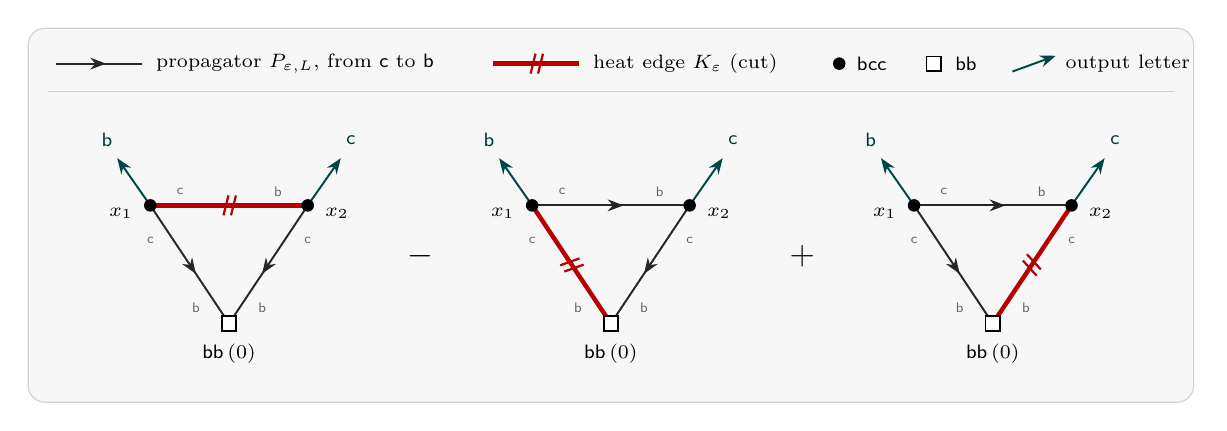
\begin{tikzpicture}[x=1cm,y=1cm]
\draw[rounded corners=6pt,draw=black!18,fill=black!3] (-2.55,-1.0) rectangle (12.25,3.75);
% legend
\draw[hfprop] (-2.2,3.3)--(-1.1,3.3); \node[anchor=west,font=\scriptsize] at (-1.05,3.3) {propagator $P_{\varepsilon,L}$, from $\mathsf c$ to $\mathsf b$};
\draw[hfheat] (3.35,3.3)--(4.45,3.3); \node[anchor=west,font=\scriptsize] at (4.5,3.3) {heat edge $K_\varepsilon$ (cut)};
\node[hfv] at (7.75,3.3) {}; \node[anchor=west,font=\scriptsize] at (7.85,3.3) {$\mathsf b\mathsf c\mathsf c$};
\node[hfo] at (8.95,3.3) {}; \node[anchor=west,font=\scriptsize] at (9.1,3.3) {$\mathsf b\mathsf b$};
\draw[hfout] (9.95,3.2)--(10.5,3.4); \node[anchor=west,font=\scriptsize] at (10.5,3.3) {output letter};
\draw[black!18] (-2.3,2.95)--(12.0,2.95);
% three terms
\bbtri{0cm}{hfheat}{hfprop}{hfprop}\node at (2.43,.85) {\large$-$};
\bbtri{4.85cm}{hfprop}{hfheat}{hfprop}\node at (7.28,.85) {\large$+$};
\bbtri{9.7cm}{hfprop}{hfprop}{hfheat}
\end{tikzpicture}
\caption{The three terms of one contraction graph in $\{\mathsf b\mathsf c\mathsf c,\mathsf b\mathsf c\mathsf c,\mathsf b\mathsf b\}_0$: the heat edge is placed on each edge in turn, with the signs $(-1)^{j-1}$ of the edge order $(12,1\mathcal O,2\mathcal O)$. The interaction vertices sit at $x_1$, $x_2$ and the insertion $\mathsf b\mathsf b$ at the origin; the output letters are $\mathsf b$ at $x_1$ and $\mathsf c$ at $x_2$.}
\label{b-00153}
\end{figure}

For an interaction density $\mathcal I$~in the action and a holomorphic local operator $\mathcal O$, the full quantum BV differential is
\begin{equation}\label{eq-1-1}
\mathbf Q=\sum_{n\geq0}\hbar^nQ_n,\qquad Q_n\mathcal O=\frac1{(n+1)!}\{\mathcal I^{\otimes(n+1)},\mathcal O\}_0 .
\end{equation}

\subsection{Where the brackets come from}\label{sec-brackets-origin}

For the holomorphic twist, \eqref{eq-C-regularized-insertion} separates into the two heat-edge terms that define \eqref{eq-A-28} \cite{Costello,semichiral,higher,BK}.

Take the holomorphic interaction density $\mathcal I$ in \eqref{eq-B-10} and a polynomial $\mathcal O$ in the zero-form fields $\mathsf c,\mathsf b,\gamma,\beta$ and their holomorphic derivatives, inserted at the origin, and write $I=\int_{\mathbb C^2}\Omega\wedge[\mathcal I]_{(0,2)}$.

\paragraph{The two terms in the insertion Ward identity.}

For these holomorphic graph integrals, the ultraviolet limit at fixed $L>0$ exists coefficientwise on smooth compactly supported external fields \cite[Theorem 5 and Corollary 4]{Wang}. Hence \eqref{eq-C-local-to-effective} applies with $I(\varepsilon)=I$ and $\mathcal O(\varepsilon)=\mathcal O$: no divergent counterterms are required. The effective interaction and transformed insertion can still receive finite corrections from the graph integrals and their collision boundaries.

For the local ultraviolet calculation write $P_\varepsilon=P_{\varepsilon,\infty}$. At finite $L$, the same calculation retains the $K_L$ term in \eqref{eq-C-finite-scale-intertwine}; scalar correlators use the infrared prescription of \eqref{eq-C-RG-correlator}. The Wick expansion with the external fields left uncontracted is
\begin{equation}\label{eq-C-expectation}
\langle\mathcal O\rangle_\varepsilon=e^{\hbar\partial_{P_\varepsilon}}\bigl(\mathcal O\,e^{I/\hbar}\bigr).
\end{equation}
Here $\langle\mathcal O\rangle_\varepsilon$ is an unnormalized functional of the remaining fields, before their final integration. The scale identity becomes
\begin{equation}\label{eq-C-scale-intertwine}
Q_{\mathrm{BV}}\,e^{\hbar\partial_{P_\varepsilon}}
=e^{\hbar\partial_{P_\varepsilon}}\,\bigl(Q_{\mathrm{BV}}+\hbar\Delta_\varepsilon\bigr).
\end{equation}
On the local insertion,
\begin{equation}\label{eq-C-two-cuts}
\begin{aligned}
e^{-I/\hbar}\bigl(Q_{\mathrm{BV}}+\hbar\Delta_\varepsilon\bigr)\bigl(\mathcal O\,e^{I/\hbar}\bigr)
={}&\underbrace{Q_{\mathrm{BV}}\mathcal O+\hbar\Delta_\varepsilon\mathcal O}_{0}
+(I,\mathcal O)_\varepsilon
+\frac1\hbar\Bigl[\underbrace{Q_{\mathrm{BV}}I+\hbar\Delta_\varepsilon I}_{0}
+\frac12(I,I)_\varepsilon\Bigr]\mathcal O\\
={}&\underbrace{(I,\mathcal O)_\varepsilon}_{\substack{\text{the action bracketed with }\mathcal O:\\ \text{heat edge between }\mathcal O\text{ and }\mathcal I}}
+\underbrace{\frac1{2\hbar}(I,I)_\varepsilon\,\mathcal O}_{\substack{\text{defect of the master equation at scale }\varepsilon:\\ \text{heat edge between }\mathcal I\text{ and }\mathcal I}}.
\end{aligned}
\end{equation}

Here $(\ ,\ )_\varepsilon$ is the BV bracket with the pairing smeared to $K_\varepsilon$. The free differential annihilates the integrated holomorphic interaction and the zero-form holomorphic input, $Q_{\mathrm{BV}}I=Q_{\mathrm{BV}}\mathcal O=0$, and a contraction of two fields at the same point vanishes, $\Delta_\varepsilon I=\Delta_\varepsilon\mathcal O=0$, because the form $d(x_1-x_2)^{-\dot+}\wedge d(x_1-x_2)^{-\dot-}$ of \eqref{eq-C-heat-spatial} is zero at $x_1=x_2$. Two terms remain, and each contains exactly one heat kernel $K_\varepsilon$. In the first, the bracket $(I,\mathcal O)_\varepsilon$ of the action with the insertion contracts a field of $\mathcal O$ with a field of one interaction vertex. In the second, $(I,I)_\varepsilon$ contracts the fields of two interaction vertices: the local interaction satisfies the classical master equation \eqref{eq-B-5} with the delta-function pairing, and $\frac12(I,I)_\varepsilon$ is its defect when the pairing is smeared to the scale $\varepsilon$. Applying \eqref{eq-C-scale-intertwine} to $\mathcal O\,e^{I/\hbar}$ therefore gives the Ward identity
\begin{equation}\label{eq-C-Ward}
Q_{\mathrm{BV}}\,\langle\mathcal O\rangle_\varepsilon
=e^{\hbar\partial_{P_\varepsilon}}
\Bigl(\Bigl[(I,\mathcal O)_\varepsilon+\frac1{2\hbar}(I,I)_\varepsilon\,\mathcal O\Bigr]e^{I/\hbar}\Bigr).
\end{equation}

The right-hand side is a sum of Feynman graphs with one heat edge, carrying $K_\varepsilon$, and propagators $P_\varepsilon$ on all other edges: the heat edge joins $\mathcal O$ to an interaction vertex in the graphs of the first term, and two interaction vertices in the graphs of the second (Figure \ref{fig-cut-origin}). In terms of the graph integrand, \eqref{eq-C-scale-intertwine} is the action of $\bar\partial$ on the product of the propagators \cite[\S2.3]{BK}: for the ordered edges $e_1,\ldots,e_E$,
\begin{equation}\label{eq-C-heat-edge-cut}
\bar\partial\bigwedge_{i=1}^{E}[P_{\varepsilon;e_i}]_\Omega
=\sum_{\substack{j=1,\ldots,E\\\mathrm{heat\ edges}}}(-1)^{j-1}
\left(\bigwedge_{i<j}[P_{\varepsilon;e_i}]_\Omega\right)
\wedge[K_{\varepsilon;e_j}]_\Omega
\wedge\left(\bigwedge_{i>j}[P_{\varepsilon;e_i}]_\Omega\right),
\end{equation}
which is the sum over $j$ in \eqref{eq-A-28}, with the sign of moving $\bar\partial$ past $j-1$ propagator one-forms.

\begin{figure}[H]
\centering
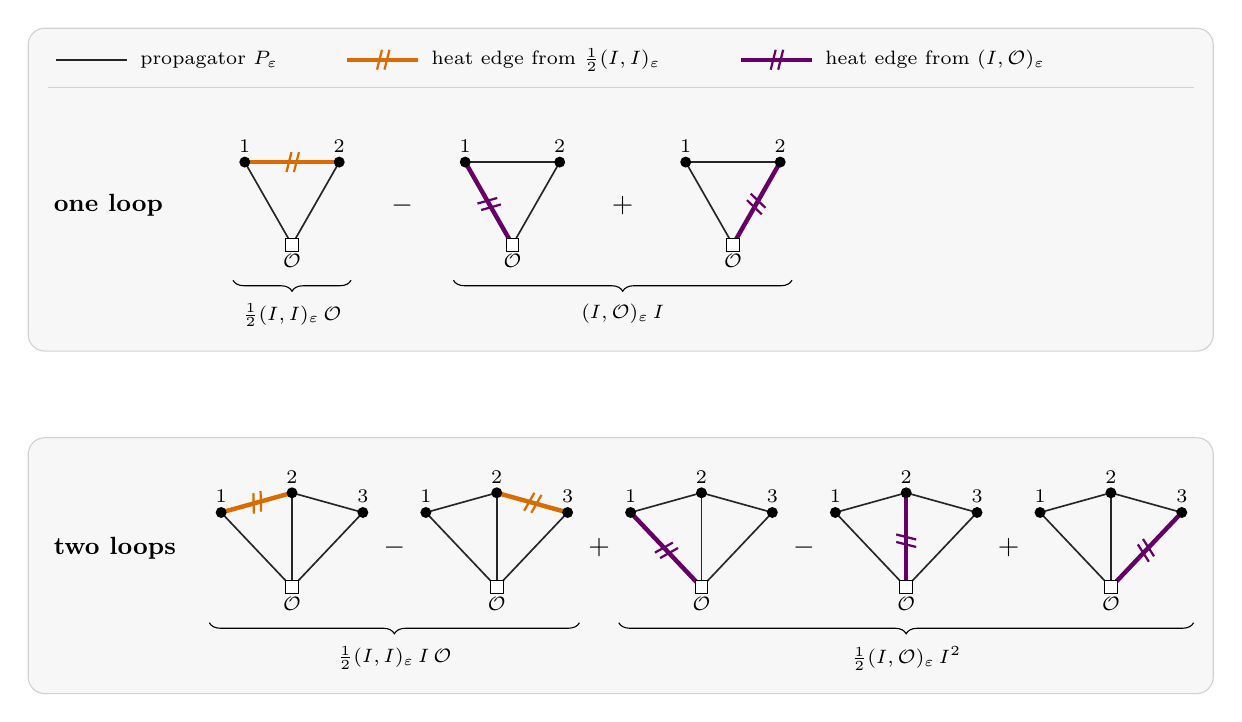
\begin{tikzpicture}[x=1cm,y=1cm]
\draw[rounded corners=6pt,draw=black!18,fill=black!3] (-2.75,-1.35) rectangle (12.3,2.75);
\draw[cutp] (-2.4,2.35)--(-1.5,2.35); \node[anchor=west,font=\scriptsize] at (-1.45,2.35) {propagator $P_\varepsilon$};
\draw[cutI] (1.3,2.35)--(2.2,2.35); \node[anchor=west,font=\scriptsize] at (2.25,2.35) {heat edge from $\tfrac12(I,I)_\varepsilon$};
\draw[cutO] (6.3,2.35)--(7.2,2.35); \node[anchor=west,font=\scriptsize] at (7.25,2.35) {heat edge from $(I,\mathcal O)_\varepsilon$};
\draw[black!18] (-2.5,2.0)--(12.05,2.0);
\node[anchor=west,font=\small\bfseries] at (-2.55,.5) {one loop};
\cutone{0.6cm}{cutI}{cutp}{cutp}\node at (2.0,.5) {$-$};
\cutone{3.4cm}{cutp}{cutO}{cutp}\node at (4.8,.5) {$+$};
\cutone{6.2cm}{cutp}{cutp}{cutO}
\draw[decorate,decoration={brace,mirror,amplitude=4pt}] (-.15,-.45)--(1.35,-.45) node[midway,below=5pt] {\scriptsize$\tfrac1{2}(I,I)_\varepsilon\,\mathcal O$};
\draw[decorate,decoration={brace,mirror,amplitude=4pt}] (2.65,-.45)--(6.95,-.45) node[midway,below=5pt] {\scriptsize$(I,\mathcal O)_\varepsilon\,I$};
\begin{scope}[yshift=-4.35cm]
\draw[rounded corners=6pt,draw=black!18,fill=black!3] (-2.75,-1.35) rectangle (12.3,1.9);
\node[anchor=west,font=\small\bfseries] at (-2.55,.5) {two loops};
\cuttwo{0.6cm}{cutI}{cutp}{cutp}{cutp}{cutp}\node at (1.9,.5) {$-$};
\cuttwo{3.2cm}{cutp}{cutI}{cutp}{cutp}{cutp}\node at (4.5,.5) {$+$};
\cuttwo{5.8cm}{cutp}{cutp}{cutO}{cutp}{cutp}\node at (7.1,.5) {$-$};
\cuttwo{8.4cm}{cutp}{cutp}{cutp}{cutO}{cutp}\node at (9.7,.5) {$+$};
\cuttwo{11.0cm}{cutp}{cutp}{cutp}{cutp}{cutO}
\draw[decorate,decoration={brace,mirror,amplitude=4pt}] (-.45,-.45)--(4.25,-.45) node[midway,below=5pt] {\scriptsize$\tfrac12(I,I)_\varepsilon\,I\,\mathcal O$};
\draw[decorate,decoration={brace,mirror,amplitude=4pt}] (4.75,-.45)--(12.05,-.45) node[midway,below=5pt] {\scriptsize$\tfrac12(I,\mathcal O)_\varepsilon\,I^2$};
\end{scope}
\end{tikzpicture}
\caption{Origin of the heat edge in $Q_1\mathcal O$ and $Q_2\mathcal O$. Dots are interaction vertices and the square is $\mathcal O$. The heat edge, marked by a cut, carries $K_\varepsilon$: between two interaction vertices (orange) it comes from the defect $\frac12(I,I)_\varepsilon$ of the master equation at the scale $\varepsilon$, and at $\mathcal O$ (violet) from the bracket $(I,\mathcal O)_\varepsilon$. The signs are $(-1)^{j-1}$ for the edge orders $(12,1\mathcal O,2\mathcal O)$ and $(12,23,1\mathcal O,2\mathcal O,3\mathcal O)$.}
\label{fig-cut-origin}
\end{figure}

\paragraph{The limit $\varepsilon\downarrow0$.}

As $\varepsilon\downarrow0$ the heat kernel $K_\varepsilon$ concentrates at coincident points and forces a connected cluster of vertices that contains the heat edge to collapse to a point. A total-collision boundary is a finite, constant-coefficient holomorphic differential operator on the coincident vertex inputs \cite[Theorem 6]{Wang}. Together the two terms of \eqref{eq-C-Ward} have a finite limit. A cluster of interaction vertices alone gives the brackets $\{\mathcal I^{\otimes k}\}_0$ of the interaction with itself. They cancel when the interaction satisfies the quantum master equation \eqref{eq-2-40}, which in the present language reads
\begin{equation}\label{eq-C-QME}
\lim_{\varepsilon\downarrow0}e^{\hbar\partial_{P_\varepsilon}}\Bigl((I,I)_\varepsilon\,e^{I/\hbar}\Bigr)=0 .
\end{equation}
At order $\hbar^0$ this is the classical master equation $(I,I)=0$ with the ordinary bracket, and at one loop it is the standard triangle graph, the gauge anomaly \eqref{eq-sum-QI}, which vanishes for $\operatorname{Tr}_R(t_A\{t_B,t_C\})=0$ (Theorem~\ref{b-00465}). A cluster that contains $\mathcal O$ and some of the interaction vertices gives a local operator at the origin, and the vertices and propagators outside the cluster reproduce the expectation value of that operator:
\begin{equation}\label{eq-C-local-Ward-identity}
\lim_{\varepsilon\downarrow0}Q_{\mathrm{BV}}\,\langle\mathcal O\rangle_\varepsilon
=\lim_{\varepsilon\downarrow0}\langle\mathbf Q\mathcal O\rangle_\varepsilon,
\qquad
\mathbf Q\mathcal O=\sum_{n\ge0}\frac{\hbar^n}{(n+1)!}\{\mathcal I^{\otimes(n+1)},\mathcal O\}_0 .
\end{equation}
This is the origin of the higher brackets \eqref{eq-A-28} and of \eqref{eq-1-1}: the term of order $\hbar^n$ collects the clusters with $n+1$ interaction vertices, summed over the heat edges of each graph as in Figure \ref{fig-cut-origin}. The combinatorial coefficients of the graphs are worked out in \cite{higher,semichiral,BK}.

\subsection{Positive Schwinger times and the operatope}\label{positive-schwinger-times-and-the-operatope}

Computing a higher bracket amounts to computing the kernels of its graphs, with the external momenta supplied by the uncontracted output letters.

The translation \eqref{eq-B-21} of the surviving letters is the source of the momentum substitution in the higher bracket \eqref{eq-A-28}: writing $\lambda_{v,+\dot a}$ for the holomorphic momentum of the surviving (output) letters at the vertex $v$, the momentum at the root $k$ is eliminated by momentum conservation, and the momenta at the integrated vertices become derivatives of their surviving letters,
\begin{equation}\label{eq-D-lambda}
\begin{gathered}\lambda_{k,+\dot a}=-\sum_{\substack{v=1,\ldots,k-1\\\mathrm{integrated\ vertices}}}\lambda_{v,+\dot a},\qquad\lambda_{v,+\dot a}\longmapsto\frac{\partial}{\partial x_v^{+\dot a}}=-\frac12\partial_{v,+\dot a}\qquad(v<k),\end{gathered}
\end{equation}
with the Leibniz rule when several letters survive at $v$. A fully contracted integrated vertex has $\lambda_v=0$.

\rthm{Proposition}{b-00169}{Current representation; external input \cite[Section 2.7, Equations (2.32)--(2.33)]{operatope}, \cite[Lemma 2, Proposition 9]{Wang}} \emph{Let $\Gamma$ have vertices $V=\{1,\ldots,k\}$, the insertion at $x_k=0$, ordered edges $I=(e_1,\ldots,e_{2n+1})$, each oriented from $e(0)$ to $e(1)$, and Schwinger times $t_e>0$. } \emph{With the source $\lambda_v$ of the output letters at $v$ \eqref{eq-D-lambda}, and the edge displacement $z_e$ generating the holomorphic derivatives of the input letters \eqref{eq-W-jet-edge}, and the edge currents $y_{e,+\dot a}$ of \eqref{eq-1-8}, the kernel $\mathcal I_\Gamma(\lambda;z)$ of the graph, defined in \eqref{eq-1-7}, is}
\begin{equation}\label{eq-C-current-delta-integral}
\begin{aligned}
\mathcal I_\Gamma(\lambda;z)
={}&(-1)^n\int_{\Delta_\Gamma}
 e^{-\sum_ez_e^{+\dot a}y_{e,+\dot a}}
 \bigwedge_{e\in I}d^2y_e\\
&\times\prod_{v<k}\prod_{\dot a=\dot+,\dot-}
\delta\!\left(\lambda_{v,+\dot a}
-\sum_{e:e(0)=v}y_{e,+\dot a}
+\sum_{e:e(1)=v}y_{e,+\dot a}\right).
\end{aligned}
\end{equation}

\emph{Here the currents obey the loop law around every oriented cycle $C$,}
\begin{equation}\label{eq-C-oriented-cycle}
\sum_{\substack{e\in C\\\mathrm{along}\ C}}t_ey_{e,+\dot a}
-\sum_{\substack{e\in C\\\mathrm{against}\ C}}t_ey_{e,+\dot a}=0.
\end{equation}
\emph{for one common set of positive Schwinger times, the same for both dotted components, and $\Delta_\Gamma$ is the set of such currents, with the orientation induced by the ultraviolet boundary \eqref{eq-UV-boundary} of the Schwinger-time cube:}
\begin{equation}\label{eq-C-projective-times}
\Delta_\Gamma=\bigcup_{(t_e)\in\mathbb{RP}^{|I|-1}_{>0}}
\Bigl\{(y_{e,+\dot a})_{e\in I}:\ %
\sum_{\substack{e\in C\\\mathrm{along}\ C}}t_ey_{e,+\dot a}
-\sum_{\substack{e\in C\\\mathrm{against}\ C}}t_ey_{e,+\dot a}=0
\ \text{ for every cycle }C\Bigr\}.
\end{equation}

We now derive this representation, following \cite{Wang,operatope}.

\subsubsection*{The heat edge and the current form}\label{sec-B-kernel}

Let $V=\{1,\ldots,n+2\}$ be the vertex set of an $n$-loop Feynman graph with $2n+1$ edges, the only case in which the integral does not vanish (Lemma~\ref{b-00180}), and order the edges as $I=(e_1,\ldots,e_{2n+1})$.

Fix $x_{n+2}=0$ and $\lambda_{n+2}=-\sum_{v<n+2}\lambda_v$.

The kernel of $\Gamma$ is the spacetime integral of \eqref{eq-A-28} with the surviving letters replaced by plane waves of holomorphic momenta $\lambda_v$. It is the integral of $\bar\partial$ of the product of propagators, which places a heat kernel on each edge in turn \cite{Wang,operatope}:
\begin{equation}\label{eq-1-7}
\begin{aligned}
\mathcal I_\Gamma(\lambda;z)
={}&(-8\pi^2)^n\lim_{\varepsilon\downarrow0}
\sum_{j=1}^{2n+1}(-1)^{j-1}
\int_{(\mathbb C^2)^{n+1}}
\left(\bigwedge_{v<n+2}\Omega_v\right)
e^{\sum_{v<n+2}\lambda_{v,+\dot a}x_v^{+\dot a}}\\
&\times\left(\bigwedge_{i<j}[P_{\varepsilon,L;e_i}]_\Omega\right)
\wedge[K_{\varepsilon;e_j}]_\Omega
\wedge\left(\bigwedge_{i>j}[P_{\varepsilon,L;e_i}]_\Omega\right)\\
={}&(-8\pi^2)^n\lim_{\varepsilon\downarrow0}
\int_{(\mathbb C^2)^{n+1}}
\left(\bigwedge_{v<n+2}\Omega_v\right)
e^{\sum_{v<n+2}\lambda_{v,+\dot a}x_v^{+\dot a}}\,
\bar\partial\left(\bigwedge_{i=1}^{2n+1}[P_{\varepsilon,L;e_i}]_\Omega\right)\bigg|_{\mathrm{UV}}\\
={}&(-1)^n(-8\pi^2)^n\lim_{\varepsilon\downarrow0}
\int_{(\mathbb C^2)^{n+1}}
\left(\bigwedge_{v<n+2}\Omega_v\right)
e^{\sum_{v<n+2}\lambda_{v,+\dot a}x_v^{+\dot a}}\\
&\times\int_{\partial_{\mathrm{UV}}[\varepsilon,L]^{2n+1}}
\bigwedge_{i=1}^{2n+1}\Bigl([K_{t_{e_i};e_i}]_\Omega
-dt_{e_i}\wedge[\bar\partial^*K_{t_{e_i};e_i}]_\Omega\Bigr),
\end{aligned}
\end{equation}
\begin{equation}\label{eq-UV-boundary}
\partial_{\mathrm{UV}}[\varepsilon,L]^{2n+1}
=\bigcup_{j=1}^{2n+1}\bigl\{t_{e_j}=\varepsilon,\ \ \varepsilon\le t_{e_i}\le L\ (i\ne j)\bigr\},
\end{equation}

In the last step each propagator is written as its Schwinger-time integral \eqref{eq-C-heat-homotopy}, and the heat edge $t_{e_j}=\varepsilon$ becomes a facet of the cube $[\varepsilon,L]^{2n+1}$. The facet carries the orientation $(-1)^{j-1}\bigwedge_{i\ne j}dt_{e_i}$, the sign of passing $\bar\partial$ through $j-1$ propagators, and collecting the $2n$ Schwinger differentials in front of the propagator forms gives $(-1)^{n(2n-1)}=(-1)^n$. The facets at $t_{e_j}=L$ carry the kernel $K_L$; they do not contribute to the local operator and are absent for $L=\infty$ (Section \ref{sec-brackets-origin}).

We can further simplify the last line of \eqref{eq-1-7} by combining the terms into one two-form.

On $e=(v,w)$, the propagator and its current coordinate are
\begin{equation}\label{eq-C-explicit-propagator}
\begin{aligned}
[P_{\varepsilon,L;e}]_\Omega
={}&-\frac{(x_v-x_w)^-_{\dot a}
 d(x_v-x_w)^{-\dot a}}{32\pi^2}
 \int_\varepsilon^L\frac{dt_e}{t_e^3}\\
&\quad\times\exp\!\left[-\frac{
 (x_v-x_w)^-_{\dot a}(x_v-x_w+z_e)^{+\dot a}}{2t_e}\right].
\end{aligned}
\end{equation}
\begin{equation}\label{eq-1-8}
y_{e,+\dot a}
=\frac{(x_{e(0)}-x_{e(1)})^-_{\dot a}}{2t_e},\qquad
 d^2y_e=dy_{e,+\dot+}\wedge dy_{e,+\dot-}.
\end{equation}
\begin{equation}\label{eq-C-current-Jacobian}
\begin{aligned}
[K_{t_e;e}]_\Omega
-dt_e\wedge[\bar\partial^*K_{t_e;e}]_\Omega
={}&-\frac{e^{-y_{e,+\dot a}
 (x_{e(0)}-x_{e(1)}+z_e)^{+\dot a}}}{8\pi^2}\,d^2y_e.
\end{aligned}
\end{equation}
\begin{equation}\label{eq-kernel-current-form}
\begin{aligned}
\mathcal I_\Gamma(\lambda;z)
={}&-\frac{1}{(8\pi^2)^{n+1}}\lim_{\varepsilon\downarrow0}
\int_{(\mathbb C^2)^{n+1}}
\left(\bigwedge_{v<n+2}\Omega_v\right)
e^{\sum_{v<n+2}\lambda_{v,+\dot a}x_v^{+\dot a}}\\
&\times\int_{\partial_{\mathrm{UV}}[\varepsilon,L]^{2n+1}}
e^{-\sum_{e\in I}y_{e,+\dot a}(x_{e(0)}-x_{e(1)}+z_e)^{+\dot a}}
\bigwedge_{e\in I}d^2y_e .
\end{aligned}
\end{equation}

Now we can integrate out $x_v^{+\dot a}$ by analytically continuing these coordinates to purely imaginary values. For real $\lambda_v$ and imaginary $z_e$, deform the Gaussian contour to imaginary $x_v^+$ and real $x_v^-$. Grouping the exponent by vertex gives~
\begin{equation}\label{eq-C-fourier-exponent}
\begin{aligned}
&\sum_{v<n+2}\lambda_{v,+\dot a}x_v^{+\dot a}
-\sum_ey_{e,+\dot a}(x_{e(0)}-x_{e(1)}+z_e)^{+\dot a}\\
&\quad=-\sum_ey_{e,+\dot a}z_e^{+\dot a}
+\sum_{v<n+2}\left(\lambda_{v,+\dot a}
-\sum_{e:e(0)=v}y_{e,+\dot a}
+\sum_{e:e(1)=v}y_{e,+\dot a}\right)x_v^{+\dot a},
\end{aligned}
\end{equation}
and each vertex integral gives a delta function,
\begin{equation}\label{eq-C-fourier-delta}
\begin{aligned}
&\int_{(i\mathbb R)^2}
\frac{dx_v^{+\dot+}\wedge dx_v^{+\dot-}}{(2\pi i)^2}
\exp\!\left[\left(\lambda_{v,+\dot a}
-\sum_{e:e(0)=v}y_{e,+\dot a}
+\sum_{e:e(1)=v}y_{e,+\dot a}\right)x_v^{+\dot a}\right]\\
&\qquad=\prod_{\dot a=\dot+,\dot-}
\delta\!\left(\lambda_{v,+\dot a}
-\sum_{e:e(0)=v}y_{e,+\dot a}
+\sum_{e:e(1)=v}y_{e,+\dot a}\right),
\end{aligned}
\end{equation}
which imposes the conservation of the currents at every vertex,
\begin{equation}\label{eq-1-9}
\sum_{e:e(0)=v}y_{e,+\dot a}
-\sum_{e:e(1)=v}y_{e,+\dot a}
=\lambda_{v,+\dot a}.
\end{equation}

Each vertex integral contributes $2(2\pi i)^2=-8\pi^2$, so the normalization is
\begin{equation*}
(-8\pi^2)^n\left(-\frac1{8\pi^2}\right)^{2n+1}(-8\pi^2)^{n+1}=1,
\end{equation*}
leaving the sign $(-1)^n$ from the Schwinger differentials. The identity extends coefficient by coefficient to the formal series in $\lambda,z$. This proves \eqref{eq-C-current-delta-integral}; the loop law \eqref{eq-C-oriented-cycle} holds because $t_ey_{e,+\dot a}=\frac12(x_{e(0)}-x_{e(1)})^-_{\dot a}$ sums to zero around a cycle.

\subsubsection*{Independent currents}\label{sec-B-network}

Choose a spanning tree $T$~of the diagram.

Its grounded incidence matrix has determinant $\pm1$, so eliminating its currents by conservation has unit Jacobian for the two dotted components.

This gives
\begin{equation}\label{eq-operatope}
\mathcal I_\Gamma(\lambda;z)
=\int_{\substack{y\in\Delta_\Gamma\\
\sum_{e:e(0)=v}y_e-\sum_{e:e(1)=v}y_e=\lambda_v}}
e^{-\sum_ey_{e,+\dot a}z_e^{+\dot a}}
\bigwedge_{e\notin T}(-dy_{e,+\dot+}\wedge dy_{e,+\dot-}).
\end{equation}

The domain $\Delta_\Gamma$ consists of the solutions of the current equations for positive ratios of the Schwinger times; its orientation is the one that the map $t\mapsto y$ induces from the boundary \eqref{eq-UV-boundary} of the Schwinger-time cube.

\rthm{Remark}{b-00176}{Circuit dictionary} Equation~\eqref{eq-C-current-delta-integral} describes an electrical network on $\Gamma$. The $y_e$ are the currents on its edges and the $\lambda_v$ the external currents injected at its vertices;

Equation \eqref{eq-1-8} is Ohm's law: the potential at the vertex $v$ is its antiholomorphic position $\frac12x^-_{v,\dot a}$, and the current through $e$ is the potential difference between its ends divided by the resistance $t_e$;

The delta functions in \eqref{eq-C-current-delta-integral} impose current conservation at every vertex, and \eqref{eq-C-oriented-cycle} is the voltage law around every loop, with resistances $t_e$;

The displacements $z_e$ generate the moments of the edge currents: each $-\partial/\partial z_e^{+\dot a}$ inserts $y_{e,+\dot a}$. At $z=0$ the kernel is therefore the oriented volume swept out by the independent currents as the ratios of the edge resistances range over $\mathbb{RP}^{|I|-1}_{>0}$, and $z_e$ is the generating source that records the expectation values of the current $y_e$.

Table \ref{tab-sum-dictionary} in Section \ref{sec-sum-circuit} collects this dictionary.

This analogy brings the series, parallel, and star--triangle transformations of circuits to the holomorphic kernels. One of our core observations is that they can be applied iteratively, transferring the sources at each step, as changes of variables on Schwinger space.

\section{Constraints and classification of $Q_n$ graphs}\label{sec-restrictions}

Only a few graphs can have a nonzero contribution to \eqref{eq-C-current-delta-integral}; they must satisfy the so-called Laman condition (Section \ref{sec-laman}). In addition, the diagrams in the four-dimensional holomorphic twist of an $\mathcal N=1$ theory separate further into a few classes. This comes from the fact that each propagator lowers the number of $\mathsf b$ and $\beta$ factors by one, while each vertex raises it by at most one. The result of this section is the classification of the graphs of $Q_n$ (Corollary~\ref{b-00247}): for the interaction \eqref{eq-B-10} with $\bar W$ of arbitrary degree, every nonzero connected graph of $Q_n$, $n\ge1$, is a fan or a spider whose arms meet at its single $\bar W$ vertex (Figure \ref{fig-sum-families}); for interactions of degree at most three, including all renormalizable $\mathcal N=1$ gauge theories, only fans contribute (Section \ref{sec-only-fans}). The same counting shows that $Q_n\mathcal O$ vanishes beyond a finite loop order (Corollary~\ref{b-00235}).

\begin{figure}[H]
\centering
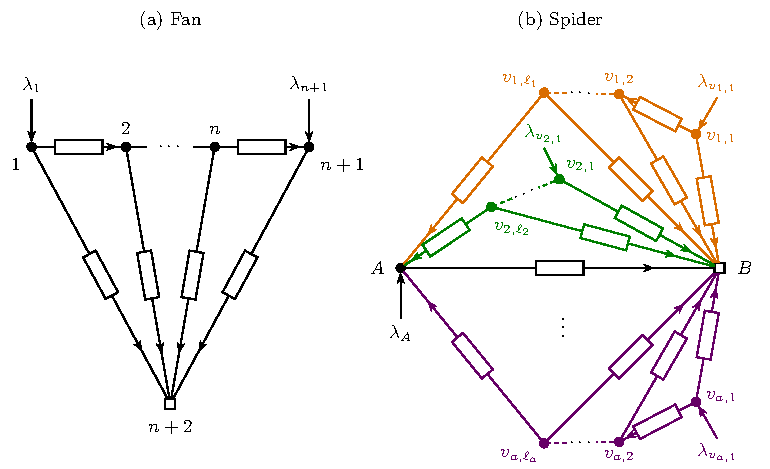
\includegraphics[width=0.82\linewidth]{figures/vec/sum_families_ab.pdf}
\caption{(a) A \emph{fan}: the interaction vertices $1,\ldots,n+1$ form a path, and each of them is joined to the insertion $n+2$ by a spoke. (b) A \emph{spider}: several such paths, the arms, meet at a vertex $A$, and every vertex, $A$ included, is joined to a second vertex $B$; in $Q_n$, $A$ is the $\bar W$ vertex and $B=\mathcal O$ (Definition~\ref{b-00380}).}
\label{fig-sum-families}
\end{figure}

\subsection{Laman constraints}\label{sec-laman}

For an induced subgraph $S\subseteq\Gamma$, write $V_S\subseteq V$ for its vertex set and $I_S\subseteq I$ for its edge set.

Some of the proofs are easier to understand in terms of a circuit diagram (Table \ref{tab-sum-dictionary}), so we sometimes provide more than one proof to illustrate the idea.

\rthm{Lemma}{b-00180}{Laman count \cite[Equation (2.22)]{operatope}, \cite[Theorem 6]{Wang}} \emph{Every nonzero graph satisfies}
\begin{equation}\label{eq-1-12}
|I|=2|V|-3 .
\end{equation}

\emph{Proof (graph integral).} The heat edge has antiholomorphic form degree two and every other propagator degree one; together they saturate the relative antiholomorphic integration directions:
\begin{equation*}
\underbrace{2}_{\text{heat kernel}}+\underbrace{(|I|-1)}_{P}
=\underbrace{2(|V|-1)}_{|V|-1\text{ points}}.
\end{equation*}

\par\vspace{-\medskipamount}\noindent\hspace*{\fill}\qedsymbol

\emph{Proof (circuit).} The resistance ratios sweep out the real components of the independent loop currents in \eqref{eq-C-current-delta-integral}:
\begin{equation*}
\underbrace{|I|-1}_{\text{independent resistance ratios}}
=\underbrace{2}_{\text{holomorphic dimension}}\,
\underbrace{(|I|-|V|+1)}_{\text{loops}}.
\end{equation*}

\par\vspace{-\medskipamount}\noindent\hspace*{\fill}\qedsymbol

\rthm{Lemma}{b-00194}{Laman bound on subgraphs \cite[Equation (2.23)]{operatope}, \cite[Proposition 5]{Wang}} \emph{Every $S\subseteq\Gamma$ with $I_S\ne\emptyset$ satisfies}
\begin{equation*}
|I_S|\le2|V_S|-3 .
\end{equation*}

\emph{Proof (graph integral).} Fix $v_0\in V_S$; the coordinates $(x_v-x_{v_0})^{-\dot a}$, $v\in V_S\setminus\{v_0\}$, give $2(|V_S|-1)$ one-form directions in the numerators of the propagators. The total form degree cannot exceed the number of one-form directions. If the heat kernel edge $K$ lies in $S$,
\begin{equation*}
|I_S|+1\le2(|V_S|-1).
\end{equation*}

If the heat edge lies outside $S$, the radial vector annihilates every internal propagator one-form \cite[Proposition 5, Lemma 2]{Wang}, \cite[Equation (2.15)]{operatope}:
\begin{equation*}
\begin{gathered}
R=\sum_{u\in V_S\setminus\{v_0\}}(x_u-x_{v_0})^{-\dot c}\frac{\partial}{\partial x_u^{-\dot c}},\\
\iota_R\bigl[-(x_v-x_w)^-_{\dot a}d(x_v-x_w)^{-\dot a}\bigr]
=-(x_v-x_w)^-_{\dot a}(x_v-x_w)^{-\dot a}=0,
\end{gathered}
\end{equation*}
so the number of holomorphic directions drops by one.
\begin{equation*}
|I_S|\le2(|V_S|-1)-1 .
\end{equation*}

\par\vspace{-\medskipamount}\noindent\hspace*{\fill}\qedsymbol

\emph{Proof (circuit).} Ohm's law is local. For connected $S$, fix the currents entering its vertices from outside. Kirchhoff's law leaves $2(|I_S|-|V_S|+1)$ independent loop-current components. The internal resistance ratios range over $\mathbb{RP}^{|I_S|-1}_{>0}$. If their variation cannot span these loop-current directions, the pullback of the loop-current volume form vanishes identically, and so does the graph kernel. Thus its form degree cannot exceed the dimension of the resistance-ratio space:
\begin{equation*}
\underbrace{2(|I_S|-|V_S|+1)}_{\text{loop-current form degree}}
\le\underbrace{|I_S|-1}_{\dim\mathbb{RP}^{|I_S|-1}_{>0}}
\quad\Longleftrightarrow\quad |I_S|\le2|V_S|-3.
\end{equation*}
The form may have lower or equal degree, but cannot be oversaturated. For disconnected $S$, apply the bound to each connected component containing an edge and add the bounds.

\par\vspace{-\medskipamount}\noindent\hspace*{\fill}\qedsymbol

Lemma~\ref{b-00194} immediately leads to:

\rthm{Corollary}{b-00188}{No self-loops or parallel edges \cite[Proposition 5]{Wang}, \cite[Section 2.1]{operatope}} \emph{A nonzero graph has no self-loop and at most one edge between any two vertices.}

\emph{Proof (propagators).} A self-loop carries $d(x_v-x_v)^{-\dot a}=0$ \cite[Section 2.3]{Wang}. Two edges between $v$ and $w$, with holomorphic shifts $z,z'$, share the one-form direction of $x_v-x_w$ \cite[Section 2.1]{operatope}:
\begin{equation}\label{eq-1-13}
\begin{aligned}
[P_{\varepsilon,L;vw}(x_v-x_w+z)]_\Omega
\wedge[P_{\varepsilon,L;vw}(x_v-x_w+z')]_\Omega&=0,\\
[K_{\varepsilon;vw}(x_v-x_w+z)]_\Omega
\wedge[P_{\varepsilon,L;vw}(x_v-x_w+z')]_\Omega&=0.
\end{aligned}
\end{equation}

\par\vspace{-\medskipamount}\noindent\hspace*{\fill}\qedsymbol

\emph{Proof (circuit).} A self-loop is shorted: $t_ey_{e,+\dot a}=0$ with $t_e>0$ gives $y_e=0$. Two resistors between the same nodes are in parallel: $t_ey_e=t_{e'}y_{e'}$, so their four current components vary in only three directions.~\hfill\qedsymbol

Corollary~\ref{b-00188} is the case $|V_S|\le2$ of Lemma~\ref{b-00194}.

These are the Laman constraints in two holomorphic dimensions \cite[Equations (2.22)--(2.23)]{operatope}, \cite[Section 3.3]{higher}, \cite[Definition 16, Proposition 5, Theorem 6]{Wang}.

\rthm{Lemma}{b-00207}{Counts at $n$ loops} \emph{A nonzero connected $n$-loop graph satisfies}
\begin{equation}\label{eq-1-11}
\begin{gathered}
|V|=n+2,\qquad |I|=2n+1,\qquad
|I|-|V|+1=n,\\
|I_S|\le2|V_S|-3\qquad(S\subseteq\Gamma,\ |V_S|\ge2).
\end{gathered}
\end{equation}

\emph{Proof.} Lemma~\ref{b-00180} and $n=|I|-|V|+1$ give the first line; Lemma~\ref{b-00194} the second.~\hfill\qedsymbol

\subsection{Cubic vertices: only fans}\label{sec-only-fans}

We now turn to the condition special to $d=4$.

By \eqref{eq-1-1}, the Feynman graphs of the loop-corrected supercharge $Q_n$ have $n+1$ interaction vertices and one insertion $\mathcal O$. We call an edge that joins an interaction vertex to $\mathcal O$ a \emph{spoke}, and write $\deg_\Gamma\mathcal O$ for the number of spokes of a graph $\Gamma$, the degree of $\mathcal O$; by Corollary~\ref{b-00188} it is at most $n+1$.

\rthm{Proposition}{b-00210}{Graphs of $Q_n$ with cubic vertices are fans} \emph{For a translation-invariant interaction $\mathcal I$ whose vertices have degree at most three, every nonzero connected $n$-loop kernel with one local-operator insertion is a fan of cubic vertices (Figure~\ref{fig-fan-family}), for $n\ge1$. (The $n=0$ case is a single edge connecting two vertices, representing the classical tree-level SUSY transformation.)} \emph{The interaction vertices form a path; each is joined to the insertion, and one output field remains at each endpoint of the path.}

\begin{figure}[H]
\centering
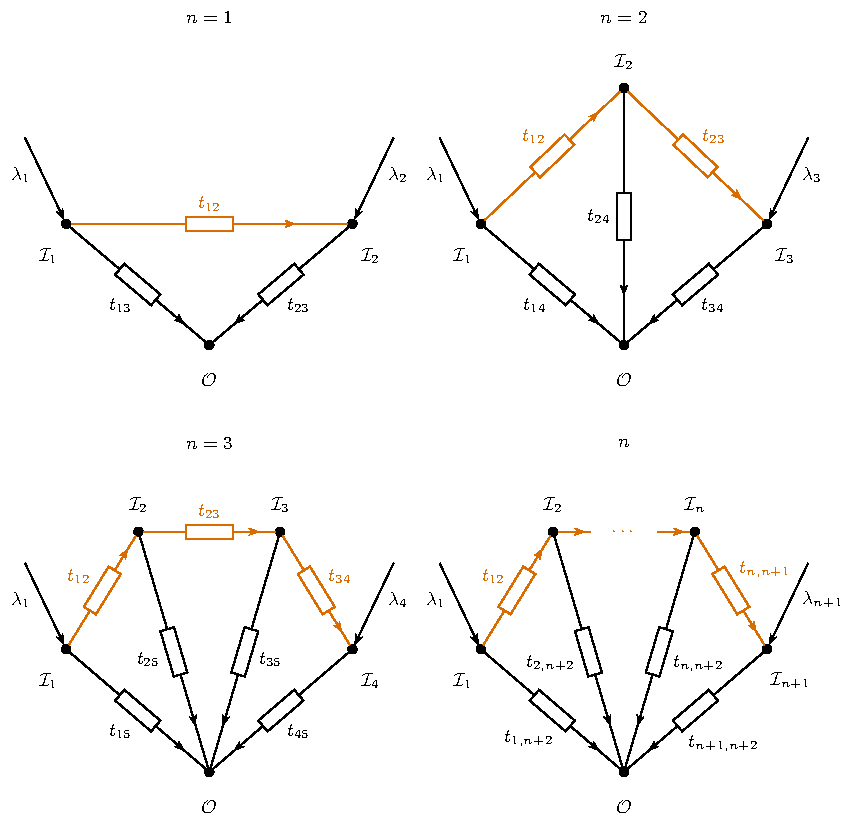
\includegraphics[width=0.91\linewidth]{figures/vec/figures-circuits-fa_fan_family.pdf}
\caption{Fans at one, two, three and $n$ loops as circuits, with the interaction path in orange, resistances $t_{vw}$ and injected currents $\lambda_1,\lambda_{n+1}$.}
\label{fig-fan-family}
\end{figure}

By Lemma~\ref{b-00207}, there are $n+1$ interaction vertices besides the insertion $\mathcal O$.

The proof of Proposition~\ref{b-00210} uses two lemmas:

\rthm{Lemma}{b-00213}{$\deg_\Gamma\mathcal O$ is maximal} \emph{In a graph of Proposition~\ref{b-00210}, $\deg_\Gamma\mathcal O=n+1$: every interaction vertex is joined to $\mathcal O$ by one edge and exactly two interaction fields remain uncontracted.}

\emph{Proof (circuit).} The uncontracted interaction fields inject the external currents. By Corollary~\ref{b-00188} and Lemma~\ref{b-00207}, with equality in the first step only for cubic vertices,
\begin{equation}\label{eq-cubiccount}
\begin{aligned}
\#(\text{sources})
&\le\underbrace{3}_{\text{degree bound}}\,
\underbrace{(n+1)}_{\mathcal I\text{ vertices}}
-\underbrace{2\bigl(2n+1-\deg_\Gamma\mathcal O\bigr)}_{\substack{\text{letters contracted between}\\\mathcal I\text{ vertices}}}
-\underbrace{\deg_\Gamma\mathcal O}_{\substack{\text{edges from }\mathcal O\\\text{to }\mathcal I\text{ vertices}}}\\
&=\underbrace{\deg_\Gamma\mathcal O}_{\substack{\le n+1\\\text{by Corollary~\ref{b-00188}}}}-n+1\le2.
\end{aligned}
\end{equation}

If there is only one source, every current is a real multiple of the source current and sweeps at most $n<2n$ dimensions; a nonzero kernel therefore has at least two sources, and both inequalities are then equalities.~\hfill\qedsymbol

\rthm{Lemma}{b-00217}{No interaction cycles} \emph{If every interaction vertex is joined to $\mathcal O$, no subgraph $S$ on interaction vertices carries a cycle.}

\emph{Proof.} A loop of resistors on the interaction nodes $V_S$, together with their $|V_S|$ spokes, gives a subcircuit on $V_S\cup\{\mathcal O\}$ with more resistors than the local count of Ohm's law allows (Lemma~\ref{b-00194}):
\begin{equation*}
|I_S|+|V_S|\ge2|V_S|>2(|V_S|+1)-3 .
\end{equation*}

\par\vspace{-\medskipamount}\noindent\hspace*{\fill}\qedsymbol

\emph{Proof of Proposition~\ref{b-00210}.} By Lemma~\ref{b-00213}, each of the $n+1$ cubic interaction nodes is wired to $\mathcal O$ by one spoke, which leaves $2n+1-(n+1)=n$ internal resistors; they close no loop (Lemma~\ref{b-00217}) and form a tree. Each node spends one terminal on its spoke and keeps at most two for internal resistors, so the tree is a chain: its interior nodes wire all three terminals, and each end keeps one free terminal, the two sources of Lemma~\ref{b-00213}.~\hfill\qedsymbol

\rthm{Corollary}{b-00222}{Renormalizable theories} \emph{For every renormalizable $\mathcal N=1$ gauge theory, massless or massive, every nonzero connected graph of $Q_n$, $n\ge1$, with one insertion $\mathcal O$ is a fan of cubic vertices.}

\emph{Proof.} The superpotential has degree at most three, and Proposition~\ref{b-00210} applies.~\hfill\qedsymbol

The fan kernel is the simplest one to evaluate. If the theory is non-renormalizable (with $\mathcal I$ of degree greater than three), other kinds of kernels can also appear; they are, however, also highly constrained.

\subsection{Superpotential vertices of higher degree: spiders}\label{sec-spider-classification}

\rthm{Proposition}{b-00225}{Superpotential vertices and antifield count} \emph{For the interaction \eqref{eq-B-10}, allow $\bar W(\gamma,\mathsf w)$ to have arbitrary degree. } \emph{Every nonzero connected $n$-loop graph of $Q_n\mathcal O$ with one insertion $\mathcal O$, $n\ge1$, contains at most one $\bar W$ vertex. } \emph{Each graph term lowers the number of $\mathsf b,\beta$ factors by $n$ plus the number of $\bar W$ vertices.}

We prove Proposition~\ref{b-00225} with the help of two lemmas.

\rthm{Lemma}{local-3f6d7139-9e21-4d1f-95cc-7d06f9c41ebc}{Antifield terminals}

\emph{Every contraction pairs a $\mathsf b$ or $\beta$ factor with a $\mathsf c$ or $\gamma$ factor. } \emph{A gauge or matter vertex of \eqref{eq-B-10} supplies one $\mathsf b$ or $\beta$ factor, a $\bar W$ vertex none.}

\emph{Proof.} A gauge or matter node, $\mathsf b\mathsf c\mathsf c$ or $\mathsf c\gamma\beta$ in \eqref{eq-B-10}, has one antifield terminal, a node of $\bar W(\gamma,\mathsf w)$ none.~\hfill\qedsymbol

\rthm{Lemma}{b-00228}{Internal edges} \emph{A nonzero connected $n$-loop graph of $Q_n$ has at least $n$ edges between interaction vertices.}

\emph{Proof.} Two resistors from $\mathcal O$ to the same interaction node would be in parallel (Corollary~\ref{b-00188}), so at most $n+1$ of the $2n+1$ resistors (Lemma~\ref{b-00207}) end at $\mathcal O$, and $2n+1-\deg_\Gamma\mathcal O\ge2n+1-(n+1)=n$ join interaction nodes.~

This is a weaker version of Lemma~\ref{b-00213}, which does not use the cubic condition.\hfill\qedsymbol

\emph{Proof of Proposition~\ref{b-00225}.} By Lemmas~\ref{local-3f6d7139-9e21-4d1f-95cc-7d06f9c41ebc} and~\ref{b-00228},
\begin{equation}\label{eq-1-15}
\begin{gathered}
\underbrace{n}_{\substack{\deg_\Gamma\mathcal O\le n+1\\
\text{at most }n+1\text{ spokes}}}
\le
\underbrace{2n+1-\deg_\Gamma\mathcal O}_{\text{internal resistors}}
\le
\underbrace{n+1-\#(\bar W\text{ vertices})}_{\substack{
\text{antifield terminals,}\\
\text{one per internal resistor}}}
\\[3pt]
\Longrightarrow\quad\#(\bar W\text{ vertices})\le1,
\end{gathered}
\end{equation}
and each of the $2n+1$ resistors takes one antifield terminal, a $\mathsf b$ or $\beta$ factor:
\begin{equation}\label{eq-antifield-loss}
\begin{aligned}
\#(\mathsf b,\beta\text{ in the output})
&=\#(\mathsf b,\beta\text{ in }\mathcal O)
  +\bigl[n+1-\#(\bar W\text{ vertices})\bigr]-(2n+1)\\
&=\#(\mathsf b,\beta\text{ in }\mathcal O)
  -n-\#(\bar W\text{ vertices}).
\end{aligned}
\end{equation}

\par\vspace{-\medskipamount}\noindent\hspace*{\fill}\qedsymbol

\rthm{Corollary}{b-00235}{Finite loop order} \emph{For $\bar W$ of any degree, or a formal power series read coefficientwise, $Q_n\mathcal O=0$ for $n>\#(\mathsf b,\beta\text{ in }\mathcal O)$, and terms with a $\bar W$ vertex vanish already for $n+1>\#(\mathsf b,\beta\text{ in }\mathcal O)$.}

\emph{Proof.} The left side of \eqref{eq-antifield-loss} is nonnegative.~\hfill\qedsymbol

Corollary~\ref{b-00235} and dimensional counting make the perturbative expansion truncate at a finite order, so that the perturbative cohomology is well defined.

\rthm{Proposition}{b-00240}{Graphs with one superpotential vertex} \emph{For the interaction \eqref{eq-B-10}, a nonzero connected $n$-loop graph of $Q_n$, $n\ge1$, with one insertion $\mathcal O$ and one $\bar W$ vertex joins $\mathcal O$ to all $n+1$ interaction vertices, for any degree of $\bar W$. } \emph{Removing $\mathcal O$ leaves a tree whose arms meet at $\bar W$.}

This type of kernel is called a spider.

\emph{Proof.} With one $\bar W$ vertex the two bounds in \eqref{eq-1-15} coincide:
\begin{equation}\label{eq-superpotential-spokes}
n\le2n+1-\deg_\Gamma\mathcal O\le n
\quad\Longrightarrow\quad
\deg_\Gamma\mathcal O=n+1,
\end{equation}
so every interaction node is wired to $\mathcal O$, and the $n$ internal resistors close no loop (Lemma~\ref{b-00217}) and form a tree. A cubic node keeps at most two internal resistors besides its spoke, so the tree branches only at the $\bar W$ node; with $a$ arms of $\ell_i$ cubic nodes,
\begin{equation}\label{eq-1-16}
\begin{gathered}
\Gamma\setminus\{\mathcal O\}
=\text{arms of lengths }\ell_1,\ldots,\ell_a\text{ meeting at }\bar W,\\
\ell_1+\cdots+\ell_a=n,\qquad\ell_i\ge1,\qquad\deg\bar W\ge a+1,
\end{gathered}
\end{equation}
where $\deg\bar W$, the number of field factors of the contributing monomial, covers the $a$ internal resistors at the $\bar W$ node and its spoke.~\hfill\qedsymbol

\rthm{Remark}{b-00246}{} With at most two arms the graph of Proposition~\ref{b-00240} is a fan; the bound $a+1\le\deg\bar W$ gives this case for $\deg\bar W\le3$.

\rthm{Corollary}{b-00247}{Graphs of $Q_n$} \emph{For the interaction \eqref{eq-B-10}, every nonzero connected graph of $Q_n$, $n\ge1$, with one insertion $\mathcal O$ is a fan, or a spider whose arms meet at its $\bar W$ vertex, a book when all its arms have length one (Definition~\ref{b-00380}); for $\deg\bar W\le3$ it is a fan.}

\emph{Proof.} Propositions~\ref{b-00210}, \ref{b-00225} and~\ref{b-00240}.~\hfill\qedsymbol

This completes the classification of the diagrams of $Q_n$.

The quantum product of Section \ref{sec-product} involves further graphs, forests of interaction trees attached to both insertions; they are classified in Section \ref{sec-dressed-definition}.

\section{Fan kernels}\label{sec-fans}

In Section~\ref{sec-BV}, we show that only the superpotential $\bar W$ of the original physical action enters the holomorphic theory; all other terms in the action of the holomorphic twist come from the kinetic BV terms.

In four dimensions, a renormalizable $\mathcal N=1$ supersymmetric gauge theory has a superpotential of degree at most three, and its holomorphic gauge and matter vertices are cubic. The fan kernels therefore determine every loop correction to the supersymmetry transformation in these theories (Corollary \ref{b-00222}), and now we evaluate them at arbitrary loop order. We state the result first. Sections~\ref{the-one-loop-triangle-diagram}--\ref{sec-fan-positive} derive it: the series and parallel reductions of a circuit become operators on kernels (Section~\ref{sec-B-local-reduction}), and iterating them along the interaction path reduces the fan to the one-loop triangle. Section~\ref{endpoint-sources-and-taylor-expansion} gives the complete Taylor expansion.

\begin{figure}[H]
\centering
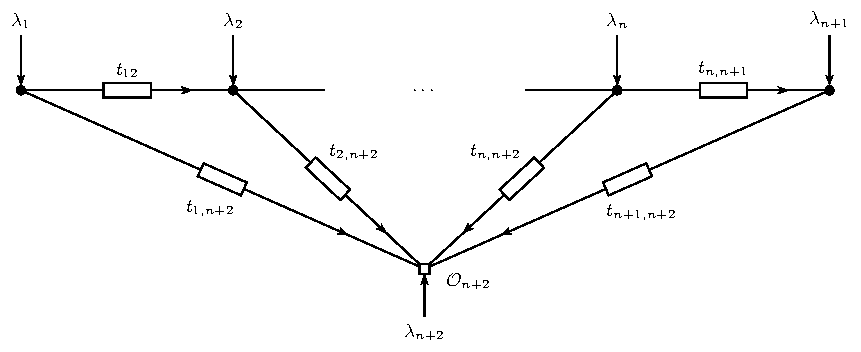
\includegraphics[width=0.91\linewidth]{figures/vec/figures-circuits-fan_general.pdf}
\caption{The $n$-loop fan circuit: a path of $n+1$ cubic interactions joined to the insertion. The resistors have resistances $t_{vw}$, and the external arrows carry the currents $\lambda_v$. The short stubs and central ellipsis indicate omitted intermediate vertices.}
\label{fig-general-fan}
\end{figure}

\rthm{Theorem}{thm-fan-kernel}{Fan kernel at every loop order} \emph{Let $\Gamma$ be the $n$-loop fan of Figure~\ref{fig-general-fan}, $n\ge1$: a path $1\to2\to\cdots\to n+1$ of interaction vertices, each joined to the insertion $n+2$ by a spoke oriented towards it. Let the path vertices carry arbitrary sources $\lambda_1,\ldots,\lambda_{n+1}$, with $\lambda_{n+2}=-\sum_{v<n+2}\lambda_v$, and the edges arbitrary displacements $z_e$. In the coordinates}
\begin{equation}\label{eq-1-37}
0<r_j<1\quad(1\leq j\leq2n-2),\qquad r_{2n-1}>0,\quad r_{2n}>0,\quad r_{2n-1}+r_{2n}<1 .
\end{equation}
\emph{the kernel \eqref{eq-operatope} is}
\begin{equation}\label{eq-1-40}
\begin{aligned}
\mathcal I_\Gamma(\lambda;z)
={}&\int_{\eqref{eq-1-37}}d^{2n}r\,
\prod_{i=1}^{n-1}\underbrace{r_{2i}
\left[\sum_{j=1}^{i}\left(\prod_{k=j}^{i-1}r_{2k-1}\right)
\lambda_{j,+\dot a_i}\right]
(\lambda_{i+1,+}{}^{\dot a_i}-y_{i+1,i+2,+}{}^{\dot a_i}(r))}_{\text{kernel factor from eliminating vertex }i}\\
&\times\underbrace{\left[\sum_{j=1}^{n}
\left(\prod_{k=j}^{n-1}r_{2k-1}\right)\lambda_{j,+\dot b}\right]
\lambda_{n+1,+}{}^{\dot b}}_{\text{final triangle factor}}
\,e^{-\sum_e y_{e,+\dot a}(r)z_e^{+\dot a}}.
\end{aligned}
\end{equation}
\emph{All currents are polynomial in $r$. Along the path,}
\begin{equation}\label{eq-1-38}
\begin{aligned}
y_{n,n+1,+\dot a}
&=r_{2n-1}\sum_{j=1}^{n}
\left(\prod_{k=j}^{n-1}r_{2k-1}\right)\lambda_{j,+\dot a}
-r_{2n}\lambda_{n+1,+\dot a},\\
y_{i,i+1,+\dot a}
&=r_{2i-1}r_{2i}\sum_{j=1}^{i}
\left(\prod_{k=j}^{i-1}r_{2k-1}\right)\lambda_{j,+\dot a}\\
&\quad-(1-r_{2i})\lambda_{i+1,+\dot a}
+(1-r_{2i})y_{i+1,i+2,+\dot a},\qquad1\le i<n.
\end{aligned}
\end{equation}
\emph{and on the spokes, by current conservation,}
\begin{equation}\label{eq-1-39}
\begin{aligned}
y_{1,n+2,+\dot a}&=\lambda_{1,+\dot a}-y_{12,+\dot a},\\
y_{i,n+2,+\dot a}&=\lambda_{i,+\dot a}+y_{i-1,i,+\dot a}-y_{i,i+1,+\dot a},
\qquad2\le i\le n,\\
y_{n+1,n+2,+\dot a}&=\lambda_{n+1,+\dot a}+y_{n,n+1,+\dot a}.
\end{aligned}
\end{equation}
\emph{For the sources and displacements of $Q_n$ in a renormalizable theory, $\lambda_2=\cdots=\lambda_n=0$, $z_{i,i+1}=0$ and $z_{i,n+2}=-z_i$, the density factorizes:}
\begin{equation}\label{eq-1-41}
\begin{aligned}
&\mathcal I_\Gamma(\lambda;z)
\big|_{\lambda_2=\cdots=\lambda_n=0,
\ z_{i,i+1}=0,\ z_{i,n+2}=-z_i}\\
&=(\lambda_{1,+\dot a}\lambda_{n+1,+}{}^{\dot a})^n
\int_{\eqref{eq-1-37}}d^{2n}r\,
\left[\prod_{j=1}^{n-1}r_{2j-1}^{n-j}r_{2j}(1-r_{2j})^{j-1}\right]
r_{2n}^{n-1}
e^{\sum_j y_{j,n+2,+\dot a}z_j^{+\dot a}}.
\end{aligned}
\end{equation}
\emph{At zero displacement the kernel is}\footnote{For $n=1,2,3$, \eqref{eq-1-42} agrees with the operatope values \cite[Equations (4.20), (4.44), (4.67)]{operatope}, for which the code \cite{LamanLoopstrap} is public, and with the fans of Gui, Wang and Williams \cite[Sections 4.4--4.6]{GWW}; at $n=1$ it is the coefficient of \cite[Equation (2.48)]{BK}.}
\begin{equation}\label{eq-1-42}
\left.\mathcal I_\Gamma(\lambda;0)\right|_{\lambda_{2,+\dot a}=\cdots=\lambda_{n,+\dot a}=0}
=\frac{(\lambda_{1,+\dot a}\lambda_{n+1,+}{}^{\dot a})^n}{(n!)^3(n+1)}.
\end{equation}
\emph{Every coefficient of the displacement expansion of \eqref{eq-1-40} at $\lambda_2=\cdots=\lambda_n=0$, for arbitrary edge displacements, is the explicit finite factorial sum \eqref{eq-fan-full-taylor}.}

The final two coordinates form a triangle; the earlier coordinates range independently over intervals. \textbf{Each $r_j$ with $j\le2n-2$ is a current-division ratio of the iteration: $r_{2i-1}$ is the fraction of the source at the eliminated vertex $i$ that the series step passes to vertex $i+1$, and $r_{2i}$ is the fraction of the merged current carried by the original spoke $(i+1,n+2)$ after the parallel merge.} The last two, $r_{2n-1}$ and $r_{2n}$, are the simplex coordinates of the final triangle, as in \eqref{eq-1-25}.

All currents are polynomial in the new coordinates, without the spanning-tree denominators that appeared in previous work (Appendix~\ref{sec-B-spanning}), so every fixed Taylor coefficient is a polynomial integral over the explicit domain \eqref{eq-1-37}, for arbitrary sources on the path.

We keep the sources $\lambda_2,\ldots,\lambda_n$ arbitrary. In a renormalizable theory, however, these $\lambda$'s are zero in $Q_n$ because there are no uncontracted letters at these vertices; only $\lambda_1$ and $\lambda_{n+1}$ (and $\lambda_{n+2}=-\sum_{v<n+2}\lambda_v$) are nonzero.~ (By Propositions~\ref{b-00225} and~\ref{b-00240}, even in a non-renormalizable theory, at most one of $\lambda_2,\ldots,\lambda_n$ is nonzero in every fan kernel considered here.)

\subsection{The one-loop triangle diagram}\label{the-one-loop-triangle-diagram}

We first review the well-known one-loop result in the circuit picture.

\begin{figure}[H]
\centering
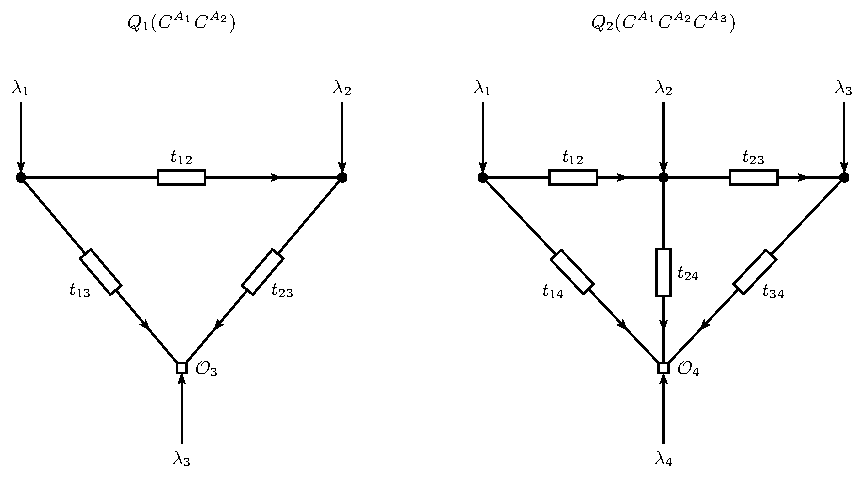
\includegraphics[width=0.92\linewidth]{figures/vec/figures-circuits-fans_low.pdf}
\caption{The one- and two-loop fan circuits. Dots are interaction vertices and the square is the local insertion. Each edge carries a resistor $t_{vw}$; $\lambda_v$ is the current injected at vertex $v$.}
\label{fig-low-fans}
\end{figure}

The vertices of the triangle are $1,2,3$, with $3$ at the origin, the insertion. With the gauge~$t_{12}+t_{13}+t_{23}=1$, current conservation and the cycle equation give\footnote{The first line of \eqref{eq-triangle-current} is read off from $\partial y_{12}/\partial\lambda_1=t_{13}$ and $\partial y_{12}/\partial\lambda_2=-t_{23}$. With $\lambda_2$ switched off, the current $\lambda_1$ enters at vertex $1$ and leaves at vertex $3$ through the two parallel paths $1\to3$ and $1\to2\to3$; the path through edge $12$, of resistance $t_{12}+t_{23}$, carries the fraction $t_{13}/(t_{12}+t_{13}+t_{23})=t_{13}$. The other two lines are just current conservation at vertices $1$ and $2$.}
\begin{equation}\label{eq-triangle-current}
\begin{aligned}
y_{12,+\dot a}&=t_{13}\lambda_{1,+\dot a}-t_{23}\lambda_{2,+\dot a},\\
y_{13,+\dot a}&=\lambda_{1,+\dot a}-y_{12,+\dot a},\\
y_{23,+\dot a}&=\lambda_{2,+\dot a}+y_{12,+\dot a}.
\end{aligned}
\end{equation}

Use simplex coordinates $r_1,r_2$ with $(t_{12},t_{13},t_{23})=(1-r_1-r_2,r_1,r_2)$.

The Jacobian is
\begin{equation}\label{b-00267}
-dy_{12,+\dot+}\wedge dy_{12,+\dot-}
=(\lambda_{1,+\dot a}\lambda_{2,+}{}^{\dot a})\,dr_1\wedge dr_2.
\end{equation}

Then
\begin{equation}\label{eq-1-25}
\begin{aligned}
\mathcal I_\triangle(\lambda;z)
&=(\lambda_{1,+\dot a}\lambda_{2,+}{}^{\dot a})
\int_0^1dr_1\int_0^{1-r_1}dr_2\,
e^{-\sum_e y_{e,+\dot b}z_e^{+\dot b}}.
\end{aligned}
\end{equation}

Expanding the exponential and integrating each monomial yields the entire displacement dependence, as in \cite[Equation (2.47)]{BK}:\footnote{As in \eqref{eq-W-jet-edge}, the displacements generate the holomorphic derivatives of the letters of $\mathcal O$.}
\begin{equation}\label{eq-1-46}
\begin{aligned}
\mathcal I_\Gamma(\lambda;z)
={}&(\lambda_{1,+\dot a}\lambda_{2,+}{}^{\dot a})\,
 e^{-\lambda_{1,+\dot a}z_{13}^{+\dot a}-\lambda_{2,+\dot a}z_{23}^{+\dot a}}\\
&\times\sum_{i,j\ge0}
\frac{[-\lambda_{1,+\dot b}(z_{12}+z_{23}-z_{13})^{+\dot b}]^i
[\lambda_{2,+\dot c}(z_{12}+z_{23}-z_{13})^{+\dot c}]^j}{(i+j+2)!}.
\end{aligned}
\end{equation}

\subsection{Local reductions as kernel operators}\label{sec-B-local-reduction}\label{sec-network}

We reduce each graph integral to an integro-differential operator acting on the kernel of a smaller graph. Each move replaces a circuit by a reduced one, whose quantities carry the superscript $\mathrm{red}$; the kernel operator of the move follows from the corresponding change of variables. The moves are local: they do not use the global solution of the circuit by a sum over spanning trees \cite[Theorem 4 and Corollary 2]{Wang}, which is recalled in Appendix~\ref{sec-B-spanning}.

\subsubsection{Series elimination}\label{local-B-series-heading}

If $v$ has only two neighbours, $u,w$, we can eliminate $v$ by first transferring the external current injected at $v$ to $u$ and $w$ (Figure~\ref{local-498490d8-748b-4aac-a672-decb922b2630}).

\begin{figure}[H]
\centering
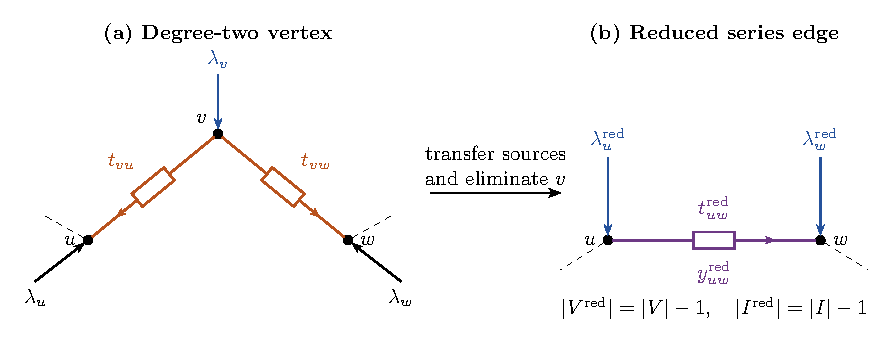
\includegraphics[width=0.95\linewidth]{figures/vec/b3-series-resistors-20261107.pdf}
\caption{Series elimination. The source at $v$ is transferred to $u,w$ as in \eqref{eq-1-64}; the loop number is unchanged.}
\label{local-498490d8-748b-4aac-a672-decb922b2630}
\end{figure}

Conservation and the voltage between them give
\begin{equation}\label{eq-B-series-derivation}
\begin{aligned}
y_{vu,+\dot a}+y_{vw,+\dot a}&=\lambda_{v,+\dot a},\\
\frac{(x_u-x_w)^-_{\dot a}}2
&=-t_{vu}y_{vu,+\dot a}+t_{vw}y_{vw,+\dot a}\\
&=t_{vw}\lambda_{v,+\dot a}-(t_{vu}+t_{vw})y_{vu,+\dot a}.
\end{aligned}
\end{equation}

For the elimination labelled $j$, take $r_j=t_{vu}/(t_{vu}+t_{vw})$.

The reduced edge $u\to w$ and transferred sources are
\begin{equation}\label{eq-1-64}
\begin{gathered}
r_j=\frac{t_{vu}}{t_{vu}+t_{vw}},\qquad
t_{uw}^{\mathrm{red}}=t_{vu}+t_{vw},\\
\lambda_{u,+\dot a}^{\mathrm{red}}
=\lambda_{u,+\dot a}+(1-r_j)\lambda_{v,+\dot a},\qquad
\lambda_{w,+\dot a}^{\mathrm{red}}
=\lambda_{w,+\dot a}+r_j\lambda_{v,+\dot a},\\
y_{vu,+\dot a}=(1-r_j)\lambda_{v,+\dot a}-y_{uw,+\dot a}^{\mathrm{red}},\qquad
y_{vw,+\dot a}=r_j\lambda_{v,+\dot a}+y_{uw,+\dot a}^{\mathrm{red}}.
\end{gathered}
\end{equation}

\subsubsection{Parallel merge}\label{local-B-parallel-heading}

Orient the $q$ parallel edges from $u$ to $w$, labelled by $j=1,\ldots,q$.

Their common voltage gives
\begin{equation}\label{eq-B-parallel-derivation}
\begin{aligned}
t_{uw}^{(j)}y_{uw,+\dot a}^{(j)}
&=\frac{(x_u-x_w)^-_{\dot a}}2,\\
y_{uw,+\dot a}^{\mathrm{red}}
&=\sum_{j=1}^q y_{uw,+\dot a}^{(j)}
=\left(\sum_{j=1}^q\frac1{t_{uw}^{(j)}}\right)
\frac{(x_u-x_w)^-_{\dot a}}2.
\end{aligned}
\end{equation}
\begin{equation}\label{eq-1-63}
\begin{gathered}
\frac1{t_{uw}^{\mathrm{red}}}=\sum_{j=1}^q\frac1{t_{uw}^{(j)}},\qquad
r_j=\frac{t_{uw}^{\mathrm{red}}}{t_{uw}^{(j)}},\qquad\sum_{j=1}^q r_j=1,\\
y_{uw,+\dot a}^{(j)}=r_jy_{uw,+\dot a}^{\mathrm{red}}.
\end{gathered}
\end{equation}

\subsubsection{The series--parallel move}\label{sec-B-kernel-recursion}

We now integrate out the eliminated vertices. Each move becomes an operator on the reduced kernel. In successive moves, derivatives act on the entire expression to their right. For the graphs built from one edge by adding vertices joined to both endpoints of an existing edge, the type~I$'$ graphs of \cite[Definition 4.12]{GWW}, which include the fans, iterating this move interprets the cube-integral recursion of \cite[Theorem 4.13]{GWW} as successive series and parallel reductions of resistors.

\rthm{Theorem}{b-01142}{Series--parallel} Let a Laman circuit have a degree-two vertex $v$, edges $vu,vw$, and an edge $uw$. Order $vu,vw$ first. After elimination, retain the other edge positions, including the merged $uw$. The current fractions satisfy $0<r_1,r_2<1$. The new circuit is still a Laman circuit.

\begin{figure}[H]
\centering
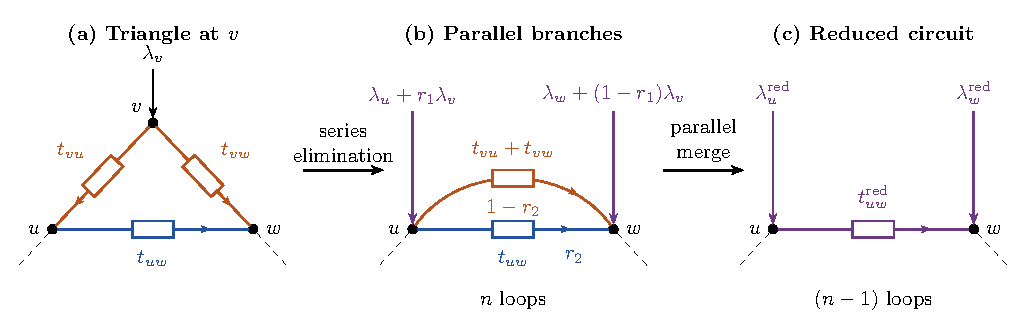
\includegraphics[width=0.96\linewidth]{figures/vec/b3-series-parallel-resistors-20261107.pdf}
\caption{Series--parallel reduction. The series branch (orange) merges with the original $uw$ edge (blue), removing one loop.}
\label{local-5fd0befa-d230-4f2f-949d-2c1a04ffe402}
\end{figure}

\begin{equation*}
\begin{gathered}
r_1=\frac{t_{vw}}{t_{vu}+t_{vw}},\qquad
r_2=\frac{t_{vu}+t_{vw}}{t_{vu}+t_{vw}+t_{uw}},\\
\lambda_u^{\mathrm{red}}=\lambda_u+r_1\lambda_v,\qquad
\lambda_w^{\mathrm{red}}=\lambda_w+(1-r_1)\lambda_v.
\end{gathered}
\end{equation*}
\begin{equation}\label{eq-kernel-series-parallel}
\begin{aligned}
\mathcal I_\Gamma(\lambda;z)
={}&\int_0^1dr_1\int_0^1dr_2\\
&\times e^{-\lambda_{v,+\dot a}(r_1z_{vu}+(1-r_1)z_{vw})^{+\dot a}}
\underbrace{r_2\lambda_{v,+\dot a}
\frac{\partial}{\partial z_{uw,\dot a}^{\mathrm{red},+}}}_{\text{local current Jacobian}}
\mathcal I_{\Gamma^{\mathrm{red}}}
(\lambda^{\mathrm{red}};z^{\mathrm{red}}).
\end{aligned}
\end{equation}
\begin{equation*}
z_{uw}^{\mathrm{red}}=r_2z_{uw}+(1-r_2)(z_{vw}-z_{vu}),\qquad
z_e^{\mathrm{red}}=z_e\quad(e\ne uw).
\end{equation*}

\begin{proofbox}
\textbf{Proof.} The resistance change fixes the orientation.
\begin{equation*}
\begin{gathered}
t_{vu}=\frac{(1-r_1)t_{uw}^{\mathrm{red}}}{1-r_2},\quad
t_{vw}=\frac{r_1t_{uw}^{\mathrm{red}}}{1-r_2},\quad
t_{uw}=\frac{t_{uw}^{\mathrm{red}}}{r_2},\\
d\!\left(\frac{t_{vu}}{t_{uw}}\right)\wedge
 d\!\left(\frac{t_{vw}}{t_{uw}}\right)
=-\frac{r_2}{(1-r_2)^3}\,dr_1\wedge dr_2.
\end{gathered}
\end{equation*}
The series step \eqref{eq-1-64}, with $r_j=1-r_1$, and the parallel merge \eqref{eq-1-63} of the new branch with the old edge $uw$, which carry the fractions $1-r_2$ and $r_2$ of the merged current, give
\begin{equation}\label{b-01151}
\begin{gathered}
y_{uw}=r_2y_{uw}^{\mathrm{red}},\qquad
y_{vu}=r_1\lambda_v-(1-r_2)y_{uw}^{\mathrm{red}},\qquad
y_{vw}=\lambda_v-y_{vu}.
\end{gathered}
\end{equation}
\begin{equation*}
\begin{aligned}
\sum_{\substack{e\in I\\\mathrm{edges}}}y_{e,+\dot a}z_e^{+\dot a}
={}&\lambda_{v,+\dot a}(r_1z_{vu}+(1-r_1)z_{vw})^{+\dot a}\\
&+\sum_{\substack{e\in I^{\mathrm{red}}\\\mathrm{edges}}}
y_{e,+\dot a}^{\mathrm{red}}z_e^{\mathrm{red},+\dot a}.
\end{aligned}
\end{equation*}

Choose a reduced spanning tree containing $uw$; conservation at fixed $\lambda$ makes $d(y_{uw,+\dot a}^{\mathrm{red}}-r_1\lambda_{v,+\dot a})$ a linear combination of the retained loop-current differentials; $\equiv$ denotes equality modulo those differentials.
\begin{equation*}
\begin{aligned}
dy_{uw,+\dot a}^{\mathrm{red}}
&=\lambda_{v,+\dot a}dr_1
+d\!\left(y_{uw,+\dot a}^{\mathrm{red}}-r_1\lambda_{v,+\dot a}\right),\\
dy_{vu,+\dot a}
&=r_2\lambda_{v,+\dot a}dr_1+y_{uw,+\dot a}^{\mathrm{red}}dr_2
-(1-r_2)d\!\left(y_{uw,+\dot a}^{\mathrm{red}}-r_1\lambda_{v,+\dot a}\right),\\
-dy_{vu,+\dot+}\wedge dy_{vu,+\dot-}
&=-r_2\left(\lambda_{v,+\dot a}y_{uw,+}^{\mathrm{red}}{}^{\dot a}\right)
 dr_1\wedge dr_2\\
&\quad+(1-r_2)\left(r_2\lambda_{v,+\dot a}dr_1+y_{uw,+\dot a}^{\mathrm{red}}dr_2\right)
 \wedge d\!\left(y_{uw,+}^{\mathrm{red}}{}^{\dot a}-r_1\lambda_{v,+}{}^{\dot a}\right)\\
&\quad-\frac{(1-r_2)^2}{2}
 d\!\left(y_{uw,+\dot a}^{\mathrm{red}}-r_1\lambda_{v,+\dot a}\right)
 \wedge d\!\left(y_{uw,+}^{\mathrm{red}}{}^{\dot a}-r_1\lambda_{v,+}{}^{\dot a}\right)\\
&\equiv-r_2\left(\lambda_{v,+\dot a}y_{uw,+}^{\mathrm{red}}{}^{\dot a}\right)
 dr_1\wedge dr_2.
\end{aligned}
\end{equation*}
\begin{equation*}
\begin{aligned}
&\lambda_{v,+\dot a}\frac{\partial}{\partial z_{uw,\dot a}^{\mathrm{red},+}}
e^{-\sum_{\substack{e\in I^{\mathrm{red}}\\\mathrm{edges}}}y_{e,+\dot b}^{\mathrm{red}}z_e^{\mathrm{red},+\dot b}}\\
&=(\lambda_{v,+\dot a}y_{uw,+}^{\mathrm{red}}{}^{\dot a})
e^{-\sum_{\substack{e\in I^{\mathrm{red}}\\\mathrm{edges}}}y_{e,+\dot b}^{\mathrm{red}}z_e^{\mathrm{red},+\dot b}}.
\end{aligned}
\end{equation*}

The two orientation signs cancel, giving \eqref{eq-kernel-series-parallel}. $\square$
\end{proofbox}

\subsection{One elimination step}\label{sec-fan-step}

The fan is reduced recursively: each step eliminates the leftmost vertex and redistributes its source between the two remaining endpoints. For the $n$-loop fan of Figure~\ref{fig-general-fan}, with path $1\to2\to\cdots\to n+1$, spokes oriented towards the insertion $n+2$, and $n\ge2$, the first step is the series--parallel move of Theorem~\ref{b-01142} at vertex $1$ (Figure~\ref{fig-fan-series-parallel-currents}).

\begin{figure}[H]
\centering
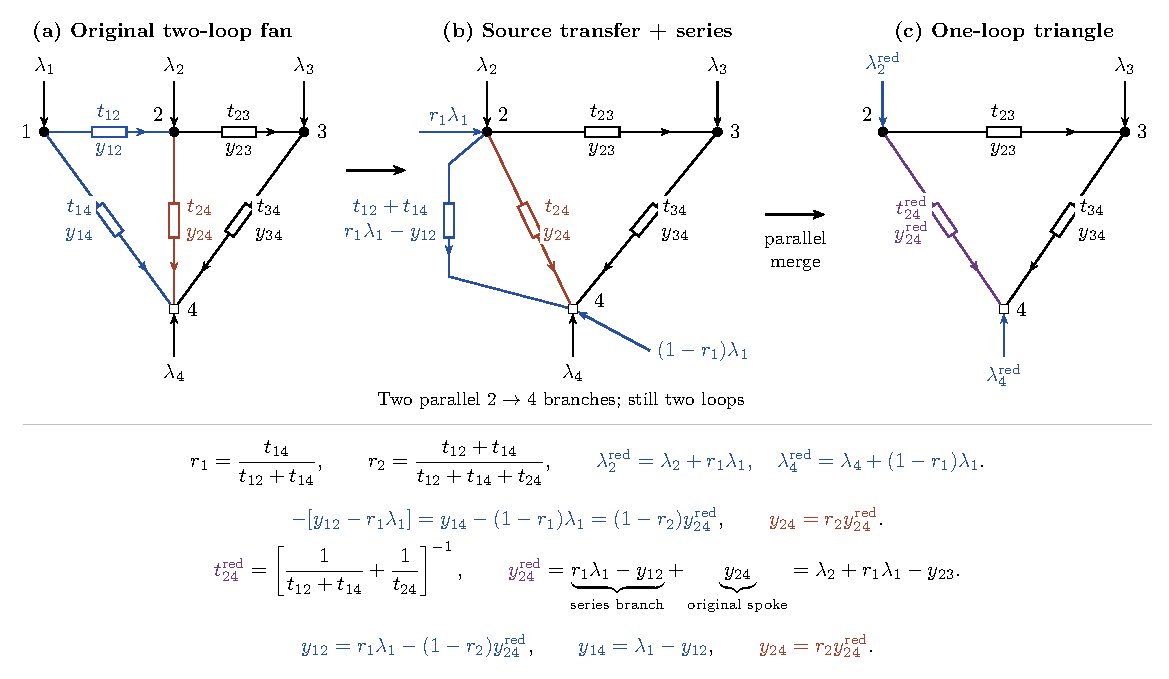
\includegraphics[width=0.96\linewidth]{figures/vec/ch4-two-loop-series-parallel-20261104.pdf}
\caption{The two-loop fan on vertices $1,2,3,4$ reduces to the triangle on $2,3,4$ (Proposition \ref{local-d52b533c-8d77-46cd-b859-f124ac49f1ea}); vertex $4$ is the insertion. Blue source arrows inject $r_1\lambda_1$ at $2$ and $(1-r_1)\lambda_1$ at insertion $4$; the series branch carries $r_1\lambda_1-y_{12}$. The parallel merge gives the triangle on $2,3,4$; the formulas beneath the circuits reconstruct the original currents.}
\label{fig-fan-series-parallel-currents}
\end{figure}

\rthm{Proposition}{local-d52b533c-8d77-46cd-b859-f124ac49f1ea}{One elimination step}

\emph{Set}
\begin{equation*}
r_1=\frac{t_{1,n+2}}{t_{12}+t_{1,n+2}},\qquad
r_2=\frac{t_{12}+t_{1,n+2}}{t_{12}+t_{1,n+2}+t_{2,n+2}},
\end{equation*}
\emph{where $r_1$ will be the fraction of $\lambda_1$ passed to vertex $2$ and $r_2$ will be the fraction of the merged spoke current carried by the original spoke $(2,n+2)$. } \emph{Eliminating vertex $1$ replaces the resistors $t_{12},t_{1,n+2},t_{2,n+2}$ by one resistor between $2$ and $n+2$ and moves the source $\lambda_1$ to the remaining endpoints:}
\begin{equation*}
t^{\mathrm{red}}_{2,n+2}=\left[\frac1{t_{12}+t_{1,n+2}}+\frac1{t_{2,n+2}}\right]^{-1},\qquad
\lambda^{\mathrm{red}}_2=\lambda_2+r_1\lambda_1,\qquad
\lambda^{\mathrm{red}}_{n+2}=\lambda_{n+2}+(1-r_1)\lambda_1 .
\end{equation*}

\emph{The removed currents follow from the reduced spoke current $y^{\mathrm{red}}_{2,n+2}=\lambda_2+r_1\lambda_1-y_{23}$:}
{\small
\begin{equation*}
y_{2,n+2}=r_2y^{\mathrm{red}}_{2,n+2},\qquad
y_{12}=r_1\lambda_1-(1-r_2)y_{2,n+2}^{\mathrm{red}}=r_1r_2\lambda_1-(1-r_2)\lambda_2+(1-r_2)y_{23},\qquad
y_{1,n+2}=\lambda_1-y_{12}.
\end{equation*}
}

\emph{With $\Gamma^{\mathrm{red}}$ the reduced fan on vertices $2,\ldots,n+2$, the kernel satisfies}
\begin{equation}\label{b-00282}
\begin{aligned}
&\mathcal I_\Gamma(\lambda;z)\\
&={}\int_0^1\!dr_1\int_0^1\!dr_2\;
e^{-\lambda_{1,+\dot a}(r_1z_{12}+(1-r_1)z_{1,n+2})^{+\dot a}}\\
&\quad\times
\underbrace{r_2\lambda_{1,+}{}^{\dot b}
\frac{\partial}{\partial z_{2,n+2}^{\mathrm{red},+\dot b}}}_{
\substack{\text{inserts the current-area Jacobian}\\
r_2(\lambda_{1,+\dot b}y^{\mathrm{red}}_{2,n+2,+}{}^{\dot b})}}
\mathcal I_{\Gamma^{\mathrm{red}}}
(\lambda^{\mathrm{red}};z^{\mathrm{red}})
.
\end{aligned}
\end{equation}

\emph{The derivative is taken before substituting}
\begin{equation*}
z^{\mathrm{red}}_{2,n+2}
=r_2z_{2,n+2}+(1-r_2)(z_{1,n+2}-z_{12}),\qquad
z^{\mathrm{red}}_e=z_e\quad(e\ne(2,n+2)).
\end{equation*}

\emph{Proof.} The kernel identity \eqref{b-00282} is \eqref{eq-kernel-series-parallel} with $(v,u,w)=(1,2,n+2)$; the currents follow from the circuit.

Conservation at $1$ and the cycle $1\to2\to n+2\to1$ give:
\begin{equation*}
y_{1,n+2}=\lambda_1-y_{12},\qquad
t_{2,n+2}y_{2,n+2}=t_{1,n+2}\lambda_1-(t_{12}+t_{1,n+2})y_{12}.
\end{equation*}

The resistors on $2\to1\to n+2$ combine in series, with resistance $t_{12}+t_{1,n+2}$, and carry
\begin{equation*}
r_1\lambda_1-y_{12}=\frac{t_{2,n+2}y_{2,n+2}}{t_{12}+t_{1,n+2}} .
\end{equation*}

In parallel with $t_{2,n+2}$ the conductances add, and the merged current $y^{\mathrm{red}}_{2,n+2}=(r_1\lambda_1-y_{12})+y_{2,n+2}$ divides as
\begin{equation*}
r_1\lambda_1-y_{12}=(1-r_2)\,y^{\mathrm{red}}_{2,n+2},\qquad
y_{2,n+2}=r_2\,y^{\mathrm{red}}_{2,n+2},
\end{equation*}
while conservation at $2$ in the reduced network gives $y^{\mathrm{red}}_{2,n+2}=\lambda^{\mathrm{red}}_2-y_{23}$. Solving for $y_{12}$ gives the stated formula.~\hfill\qedsymbol

The next step acts on vertex $2$ with the reduced source $\lambda_2+r_1\lambda_1$ and the reduced spoke $t^{\mathrm{red}}_{2,n+2}$. The iteration eventually reaches one loop.

\subsection{Fan kernels from the one-loop kernel}\label{sec-fan-positive}\label{sec-B-fan-reduction}

For $n\ge2$, iterating Proposition~\ref{local-d52b533c-8d77-46cd-b859-f124ac49f1ea} along the interaction path, at vertex $1$, then vertex $2$, and so on, reduces the fan to the triangle (Figure~\ref{local-B4-fan-chain}). Repeated application of \eqref{eq-kernel-series-parallel} gives integral--derivative operators acting on the known triangle kernel \eqref{eq-1-25}:
\begin{equation}\label{eq-fan-operator-product}
\begin{aligned}
\mathcal I_\Gamma(\lambda;z)
={}&\left[
\prod_{i=1}^{n-1}
\left(
\int_0^1dr_{2i-1}\int_0^1dr_{2i}\,
e^{-\lambda_{i,+\dot a}^{\mathrm{red}}
[r_{2i-1}z_{i,i+1}+(1-r_{2i-1})z_{i,n+2}^{\mathrm{red}}]^{+\dot a}}
\right.\right.\\[-2pt]
&\left.\left.\hspace{40mm}\times
r_{2i}\lambda_{i,+}^{\mathrm{red}}{}^{\dot b}
\frac{\partial}{\partial z_{i+1,n+2}^{\mathrm{red},+\dot b}}
\right)\right]
\underbrace{\mathcal I_\triangle
(\lambda^{\mathrm{red}};z^{\mathrm{red}})}_{\text{vertices }n,n+1,n+2}.
\end{aligned}
\end{equation}

The factor $i=1$ acts outermost; $\mathrm{red}$ refers to the indicated stage, and each derivative acts on everything to its right before that stage's displacement substitution.

\begin{figure}[H]
\centering
\begin{tikzpicture}
\node[anchor=south west,inner sep=0] (img) at (0,0) {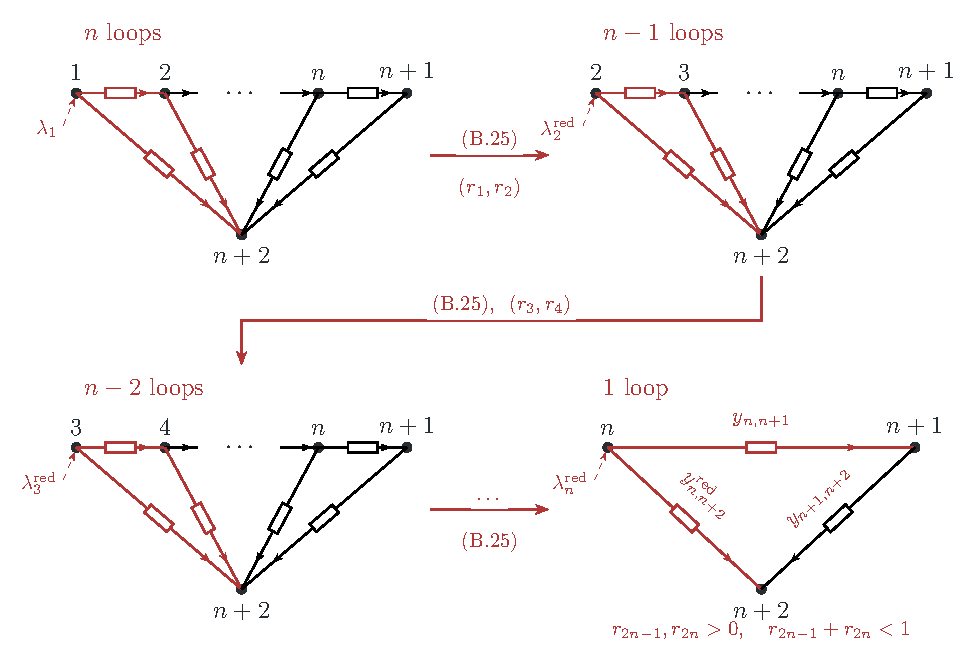
\includegraphics[width=0.96\linewidth]{figures/vec/b4-general-fan-chain-20261108.pdf}};
\begin{scope}[x={(img.south east)},y={(img.north west)}]
\node[fill=white,inner sep=1pt,minimum width=0.066\linewidth,minimum height=2.4ex,font=\footnotesize,text=blue!50!black] at (0.5004,0.7889) {\eqref{eq-kernel-series-parallel}};
\node[fill=white,inner sep=1pt,minimum width=0.072\linewidth,minimum height=2.4ex,font=\footnotesize,text=blue!50!black] at (0.4733,0.5397) {\eqref{eq-kernel-series-parallel},};
\node[fill=white,inner sep=1pt,minimum width=0.066\linewidth,minimum height=2.4ex,font=\footnotesize,text=blue!50!black] at (0.5004,0.1824) {\eqref{eq-kernel-series-parallel}};
\end{scope}
\end{tikzpicture}
\caption{The operators in \eqref{eq-kernel-series-parallel} remove vertices $1,2,\ldots,n-1$, leaving the one-loop kernel. Source transfer follows the arrows; evaluation and current reconstruction start from the final triangle and run backwards.}
\label{local-B4-fan-chain}
\end{figure}

The sources passed inward obey the following recurrence, with empty products equal to one:
\begin{equation}\label{eq-B-fan-first-cycle}
\begin{aligned}
\lambda_{1,+\dot a}^{\mathrm{red}}&=\lambda_{1,+\dot a},\\
\lambda_{i+1,+\dot a}^{\mathrm{red}}
&=\lambda_{i+1,+\dot a}+r_{2i-1}\lambda_{i,+\dot a}^{\mathrm{red}}\\
&=\lambda_{i+1,+\dot a}
+\sum_{\substack{1\le j\le i\\\mathrm{vertices}}}
\left(\prod_{k=j}^{i}r_{2k-1}\right)\lambda_{j,+\dot a}\\
&=\sum_{\substack{1\le j\le i+1\\\mathrm{vertices}}}
\left(\prod_{k=j}^{i}r_{2k-1}\right)\lambda_{j,+\dot a},
\qquad 1\le i<n.
\end{aligned}
\end{equation}

\begin{proofbox}
\textbf{Proof of \eqref{eq-1-40}.} Every kernel in \eqref{eq-fan-operator-product} depends on the displacements only through the exponential $e^{-\sum_ey_{e,+\dot a}z_e^{+\dot a}}$. Each derivative $\partial/\partial z$ therefore reads off a current $y$, and the currents are solved completely by iterating backwards from the triangle. The proof has three steps.

\medskip\noindent\textbf{Step 1: the first two operators.} The first factor of \eqref{eq-fan-operator-product} is \eqref{b-00282}; for $n\ge3$ the second is the same formula applied to the smaller fan at $(v,u,w)=(2,3,n+2)$. The first derivative acts on the phase of the second factor and on its displacement substitution:
\begin{equation}\label{eq-B-fan-second-fractions}
\begin{aligned}
&r_2\lambda_{1,+}{}^{\dot a}
\frac{\partial}{\partial z_{2,n+2}^{\mathrm{red},+\dot a}}
e^{-\lambda_{2,+\dot b}^{\mathrm{red}}
(r_3z_{23}+(1-r_3)z_{2,n+2}^{\mathrm{red}})^{+\dot b}}\\
&\quad=r_2(1-r_3)
\lambda_{1,+\dot a}\lambda_{2,+}^{\mathrm{red}}{}^{\dot a}
e^{-\lambda_{2,+\dot b}^{\mathrm{red}}
(r_3z_{23}+(1-r_3)z_{2,n+2}^{\mathrm{red}})^{+\dot b}},\\[3pt]
&z_{3,n+2}^{\mathrm{red}}
=r_4z_{3,n+2}+(1-r_4)(z_{2,n+2}^{\mathrm{red}}-z_{23}),\\
&\frac{\partial}{\partial z_{2,n+2}^{\mathrm{red},+\dot a}}
\mathcal I_{(\Gamma^{\mathrm{red}})^{\mathrm{red}}}
= (1-r_4)\frac{\partial}{\partial z_{3,n+2}^{\mathrm{red},+\dot a}}
\mathcal I_{(\Gamma^{\mathrm{red}})^{\mathrm{red}}}.
\end{aligned}
\end{equation}
By the Leibniz rule, the first operator becomes the bracket $r_2[(1-r_3)\lambda_{1,+\dot a}\lambda_{2,+}^{\mathrm{red}}{}^{\dot a}+(1-r_4)\lambda_{1,+}{}^{\dot a}\partial/\partial z_{3,n+2}^{\mathrm{red},+\dot a}]$ in the second equality of \eqref{eq-fan-chain} below. Its derivative reads off $y^{\mathrm{red}}_{3,n+2}$ from the exponential of the remaining kernel, as in \eqref{eq-fan-kernel-recursion}, and the two terms of the bracket add up to the current on the reduced spoke $(2,n+2)$, by Proposition~\ref{local-d52b533c-8d77-46cd-b859-f124ac49f1ea} applied at vertex $2$:
\begin{equation*}
(1-r_3)\lambda^{\mathrm{red}}_{2,+\dot a}+(1-r_4)y^{\mathrm{red}}_{3,n+2,+\dot a}
=\lambda^{\mathrm{red}}_{2,+\dot a}-y_{23,+\dot a}
=y^{\mathrm{red}}_{2,n+2,+\dot a}.
\end{equation*}
The first two inserted-current factors are therefore
\begin{equation*}
\begin{aligned}
r_2\lambda_{1,+\dot a}y^{\mathrm{red}}_{2,n+2,+}{}^{\dot a}
&=r_2\lambda_{1,+\dot a}
(\lambda_{2,+}{}^{\dot a}-y_{23,+}{}^{\dot a}(r)),\\
r_4\lambda^{\mathrm{red}}_{2,+\dot a}y^{\mathrm{red}}_{3,n+2,+}{}^{\dot a}
&=r_4(\lambda_{2,+\dot a}+r_1\lambda_{1,+\dot a})
(\lambda_{3,+}{}^{\dot a}-y_{34,+}{}^{\dot a}(r)).
\end{aligned}
\end{equation*}
The first two reductions give the first two equalities of the chain below; their iteration gives the rest. In each term, take the displayed derivatives first, then apply the displacement substitutions from the last reduction to the first. For $n=2$, the first reduced kernel is the triangle \eqref{eq-1-25}, so the second reduction is omitted.
\begin{equation}\label{eq-fan-chain}
\begin{aligned}
&\mathcal I_\Gamma(\lambda;z)\\
&={}\int_0^1\!dr_1\int_0^1\!dr_2\;
e^{-\lambda_{1,+\dot a}(r_1z_{12}+(1-r_1)z_{1,n+2})^{+\dot a}}\\
&\quad\times
\underbrace{r_2\lambda_{1,+}{}^{\dot b}
\frac{\partial}{\partial z_{2,n+2}^{\mathrm{red},+\dot b}}}_{
\substack{\text{inserts the current-area Jacobian}\\
r_2(\lambda_{1,+\dot b}y^{\mathrm{red}}_{2,n+2,+}{}^{\dot b})}}
\underbrace{\mathcal I_{\Gamma^{\mathrm{red}}}
(\lambda^{\mathrm{red}};z^{\mathrm{red}})}_{(n-1)\text{-loop kernel}}
\\[6pt]
&={}\int_0^1\!dr_1\int_0^1\!dr_2
\int_0^1\!dr_3\int_0^1\!dr_4\;
e^{-\lambda_{1,+\dot a}(r_1z_{12}+(1-r_1)z_{1,n+2})^{+\dot a}}\\
&\quad\times
e^{-\lambda^{\mathrm{red}}_{2,+\dot a}(r_3z_{23}+(1-r_3)z^{\mathrm{red}}_{2,n+2})^{+\dot a}}\\
&\quad\times\underbrace{r_2\left[
(1-r_3)\lambda_{1,+\dot a}\lambda^{\mathrm{red}}_{2,+}{}^{\dot a}
+(1-r_4)\lambda_{1,+}{}^{\dot b}
\frac{\partial}{\partial z_{3,n+2}^{\mathrm{red},+\dot b}}
\right]}_{\substack{\text{inserts the first current-area Jacobian}\\
r_2(\lambda_{1,+\dot b}y^{\mathrm{red}}_{2,n+2,+}{}^{\dot b})}}\\
&\quad\times
\underbrace{r_4\lambda^{\mathrm{red}}_{2,+}{}^{\dot c}
\frac{\partial}{\partial z_{3,n+2}^{\mathrm{red},+\dot c}}}_{
\substack{\text{inserts the current-area Jacobian}\\
r_4(\lambda^{\mathrm{red}}_{2,+\dot c}y^{\mathrm{red}}_{3,n+2,+}{}^{\dot c})}}
\underbrace{\mathcal I_{(\Gamma^{\mathrm{red}})^{\mathrm{red}}}\!\left(
\begin{gathered}
\lambda_3+r_3\lambda_2^{\mathrm{red}},\lambda_4,\ldots,\lambda_{n+1},\\
\lambda_{n+2}+(1-r_1)\lambda_1\\
+(1-r_3)\lambda_2^{\mathrm{red}};z^{\mathrm{red}}
\end{gathered}\right)}_{(n-2)\text{-loop kernel}}
\\[6pt]
&={}\cdots\;=\;\text{the right-hand side of \eqref{eq-1-40}}.
\end{aligned}
\end{equation}

\medskip\noindent\textbf{Step 2: evaluation from the triangle outward.} The innermost factor of \eqref{eq-fan-operator-product} is the one-loop kernel \eqref{eq-1-25}, relabelled to $n,n+1,n+2$:
\begin{equation}\label{eq-B-fan-second-merge}
\begin{aligned}
\mathcal I_\triangle(\lambda^{\mathrm{red}};z^{\mathrm{red}})
={}&(\lambda_{n,+\dot a}^{\mathrm{red}}\lambda_{n+1,+}{}^{\dot a})
\int_0^1dr_{2n-1}\int_0^{1-r_{2n-1}}dr_{2n}\,
e^{-\sum_{\substack{e\in\triangle_1\\\mathrm{edges}}}y_{e,+\dot b}^{\mathrm{red}}z_e^{\mathrm{red},+\dot b}},\\
y_{n,n+1,+\dot a}&=r_{2n-1}\lambda_{n,+\dot a}^{\mathrm{red}}
-r_{2n}\lambda_{n+1,+\dot a}.
\end{aligned}
\end{equation}
Apply the operators in the order $i=n-1,n-2,\ldots,1$. Fix the inner integration ratios and sources; the factors already obtained are independent of the displacements, so the next derivative acts on their exponential and reads off the current on the reduced spoke $(i+1,n+2)$:
\begin{equation}\label{eq-fan-kernel-recursion}
\begin{aligned}
&r_{2i}\lambda_{i,+}^{\mathrm{red}}{}^{\dot a}
\frac{\partial}{\partial z_{i+1,n+2}^{\mathrm{red},+\dot a}}
e^{-\sum_{\substack{e\in I^{\mathrm{red}}\\\mathrm{edges}}}
y_{e,+\dot b}^{\mathrm{red}}z_e^{\mathrm{red},+\dot b}}\\
&\quad=r_{2i}\bigl(\lambda_{i,+\dot a}^{\mathrm{red}}
y_{i+1,n+2,+}^{\mathrm{red}}{}^{\dot a}\bigr)
e^{-\sum_{\substack{e\in I^{\mathrm{red}}\\\mathrm{edges}}}
y_{e,+\dot b}^{\mathrm{red}}z_e^{\mathrm{red},+\dot b}}.
\end{aligned}
\end{equation}
Multiplying by the phase of the vertex being restored and substituting the reduced displacement gives
\begin{equation*}
\begin{aligned}
&\lambda_{i,+\dot a}^{\mathrm{red}}
[r_{2i-1}z_{i,i+1}+(1-r_{2i-1})z_{i,n+2}^{\mathrm{red}}]^{+\dot a}\\
&\quad+y_{i+1,n+2,+\dot a}^{\mathrm{red}}
[r_{2i}z_{i+1,n+2}+(1-r_{2i})(z_{i,n+2}^{\mathrm{red}}-z_{i,i+1})]^{+\dot a}\\
&=\bigl[r_{2i-1}\lambda_{i,+\dot a}^{\mathrm{red}}
-(1-r_{2i})y_{i+1,n+2,+\dot a}^{\mathrm{red}}\bigr]z_{i,i+1}^{+\dot a}\\
&\quad+\bigl[(1-r_{2i-1})\lambda_{i,+\dot a}^{\mathrm{red}}
+(1-r_{2i})y_{i+1,n+2,+\dot a}^{\mathrm{red}}\bigr]z_{i,n+2}^{\mathrm{red},+\dot a}
+r_{2i}y_{i+1,n+2,+\dot a}^{\mathrm{red}}z_{i+1,n+2}^{+\dot a}.
\end{aligned}
\end{equation*}
The coefficients of the three displacements are the restored currents $y_{i,i+1}$, $y^{\mathrm{red}}_{i,n+2}$ and $y_{i+1,n+2}$: the new series branch carries $(1-r_{2i})y_{i+1,n+2}^{\mathrm{red}}$, and the old spoke carries $r_{2i}y_{i+1,n+2}^{\mathrm{red}}$. Conservation at $i+1$ identifies the factor inserted by the derivative; the term $r_{2i-1}\lambda_i^{\mathrm{red}}$ drops out of the contraction, since $\lambda_{+\dot a}\lambda_{+}{}^{\dot a}=0$:
\begin{equation}\label{eq-B-fan-first-merge}
\begin{aligned}
y_{i+1,n+2,+\dot a}^{\mathrm{red}}
&=\lambda_{i+1,+\dot a}+r_{2i-1}\lambda_{i,+\dot a}^{\mathrm{red}}
-y_{i+1,i+2,+\dot a},\\
r_{2i}\lambda_{i,+\dot a}^{\mathrm{red}}
y_{i+1,n+2,+}^{\mathrm{red}}{}^{\dot a}
&=r_{2i}\lambda_{i,+\dot a}^{\mathrm{red}}
\bigl(\lambda_{i+1,+}{}^{\dot a}-y_{i+1,i+2,+}{}^{\dot a}\bigr),
\qquad 1\le i<n.
\end{aligned}
\end{equation}
Each operator thus multiplies the displacement-independent factors by this contraction and restores one more circuit. The resulting nested integral is \eqref{eq-1-40}: insert the source sum \eqref{eq-B-fan-first-cycle}; the interval pairs come from \eqref{eq-kernel-series-parallel}, and the final simplex comes from \eqref{eq-B-fan-second-merge}.

\medskip\noindent\textbf{Step 3: the currents.} The currents are now solved backwards: the triangle gives $y_{n,n+1}$, and the coefficient of $z_{i,i+1}$ in Step 2 gives $y_{i,i+1}$ in terms of $y_{i+1,i+2}$,
\begin{equation}\label{eq-B-fan-general-fractions}
\begin{aligned}
y_{n,n+1,+\dot a}
&=r_{2n-1}\lambda_{n,+\dot a}^{\mathrm{red}}-r_{2n}\lambda_{n+1,+\dot a},\\
y_{i,i+1,+\dot a}
&=r_{2i-1}\lambda_{i,+\dot a}^{\mathrm{red}}-(1-r_{2i})y_{i+1,n+2,+\dot a}^{\mathrm{red}}\\
&=r_{2i-1}r_{2i}\lambda_{i,+\dot a}^{\mathrm{red}}
-(1-r_{2i})\lambda_{i+1,+\dot a}+(1-r_{2i})y_{i+1,i+2,+\dot a},\qquad i=n-1,\ldots,1.
\end{aligned}
\end{equation}
Inserting \eqref{eq-B-fan-first-cycle} gives \eqref{eq-1-38}. The coordinates are the resistance ratios $r_{2i-1}=t^{\mathrm{red}}_{i,n+2}/(t_{i,i+1}+t^{\mathrm{red}}_{i,n+2})$ and $r_{2i}=(t_{i,i+1}+t^{\mathrm{red}}_{i,n+2})/(t_{i,i+1}+t^{\mathrm{red}}_{i,n+2}+t_{i+1,n+2})$ of Theorem~\ref{b-01142}; the first line is the triangle \eqref{eq-triangle-current} with $t_{13},t_{23}$ replaced by $t^{\mathrm{red}}_{n,n+2}=r_{2n-1}$ and $t_{n+1,n+2}=r_{2n}$. The spoke currents \eqref{eq-1-39} follow from conservation in the restored fan. This reflects the order of our iteration: the path currents are fixed first, backward from $y_{n,n+1}$ to $y_{12}$, and current conservation at each path vertex then determines every spoke current.

For $n=1$, the operator product is empty and gives \eqref{eq-1-25}; for $n=2$, the single operator restores the two-loop circuit of Figure~\ref{fig-fan-series-parallel-currents}. $\square$
\end{proofbox}

\subsection{Final Taylor expansion}\label{endpoint-sources-and-taylor-expansion}

As noted above, in the computation of $Q_n$ in renormalizable theories, the middle $\lambda$'s are all zero.

Moreover, the interaction vertices carry no derivatives, so only the holomorphic derivatives of the letters of $\mathcal O$ generate displacements. These sit on the spokes: $z_{i,i+1}=0$ and $z_{i,n+2}=-z_i$, where $z_i$ displaces the letter contracted on spoke $i$. The density of \eqref{eq-1-40} then factorizes into \eqref{eq-1-41}: since $\lambda_{1,+\dot a}\lambda_{1,+}{}^{\dot a}=0$, only the $\lambda_{n+1}$ term of $y_{i+1,i+2}$ in \eqref{eq-1-38}, $-r_{2n}\prod_{k=i+1}^{n-1}(1-r_{2k})\,\lambda_{n+1}$, contributes to the factor of vertex $i$.

The exponential in \eqref{eq-1-41} translates the two endpoint fields. Substituting the currents \eqref{eq-1-38}--\eqref{eq-1-39} gives
\begin{equation}\label{eq-fan-output-translation}
\sum_{j=1}^{n+1}y_{j,n+2,+\dot a}(r)z_j^{+\dot a}
=\lambda_{1,+\dot a}x_1^{+\dot a}(r,z)
+\lambda_{n+1,+\dot a}x_{n+1}^{+\dot a}(r,z),
\end{equation}
where the translated positions are
\begin{equation}\label{eq-fan-output-points}
\begin{aligned}
x_1^{+\dot a}(r,z)
={}&\sum_{j=1}^{n}(1-r_{2j-1})
\left(\prod_{k=1}^{j-1}r_{2k-1}\right)\\
&\times\left[
\left(\prod_{k=1}^{j-1}(1-r_{2k})\right)z_1^{+\dot a}
+\sum_{i=2}^{j}r_{2i-2}
\left(\prod_{k=i}^{j-1}(1-r_{2k})\right)z_i^{+\dot a}
\right]\\
&+\left(\prod_{k=1}^{n}r_{2k-1}\right)z_{n+1}^{+\dot a},\\[3pt]
x_{n+1}^{+\dot a}(r,z)
={}&r_{2n}\left[
\left(\prod_{k=1}^{n-1}(1-r_{2k})\right)z_1^{+\dot a}
+\sum_{i=2}^{n}r_{2i-2}
\left(\prod_{k=i}^{n-1}(1-r_{2k})\right)z_i^{+\dot a}
\right]\\
&+(1-r_{2n})z_{n+1}^{+\dot a}.
\end{aligned}
\end{equation}

We now give the Taylor expansion in explicit form, ready for direct use in the machine enumeration of the later sections.

The monomial moments on the parameter domain are
\begin{equation}\label{eq-1-44}
\int_{\eqref{eq-1-37}}dr_1\cdots dr_{2n}\,\prod_{j=1}^{2n}r_j^{m_j}=\frac{m_{2n-1}!\,m_{2n}!}{(m_{2n-1}+m_{2n}+2)!}\prod_{j=1}^{2n-2}\frac1{m_j+1}.
\end{equation}

Grouping by the total displacement degree $m$, the full Taylor expansion is
\begin{equation}\label{eq-fan-full-taylor}
\begin{aligned}
&\left.\mathcal I_\Gamma(\lambda;z)
\right|_{\lambda_2=\cdots=\lambda_n=0}\\
&=(\lambda_{1,+\dot a}\lambda_{n+1,+}{}^{\dot a})^n
\sum_{m=0}^{\infty}
\sum_{\substack{r_0,s_0,r_{ik},s_i\ge0\\
r_0+s_0+\sum_{i=1}^ns_i+\sum_{k=1}^n\sum_{i=1}^kr_{ik}=m}}\\
&\quad\times
\frac{[-\lambda_{1,+\dot b}z_{1,n+2}^{+\dot b}]^{r_0}
[-\lambda_{n+1,+\dot c}z_{n+1,n+2}^{+\dot c}]^{s_0}}
{r_0!s_0!}\\
&\quad\times\prod_{1\le i\le k\le n}
\frac{\left[-\lambda_{1,+\dot d}
(z_{i,i+1}+z_{i+1,n+2}-z_{i,n+2})^{+\dot d}\right]^{r_{ik}}}
{r_{ik}!}\\
&\quad\times\prod_{i=1}^n
\frac{\left[\lambda_{n+1,+\dot e}
(z_{i,i+1}+z_{i+1,n+2}-z_{i,n+2})^{+\dot e}\right]^{s_i}}
{s_i!}\\
&\quad\times
\frac{\left(\sum_{i=1}^nr_{in}\right)!
\left(n-1+\sum_{i=1}^ns_i\right)!}
{\left(n+1+\sum_{i=1}^nr_{in}+\sum_{i=1}^ns_i\right)!}\\
&\quad\times\prod_{j=1}^{n-1}
\frac{1}{n-j+1+\sum_{k=j}^{n}\sum_{i=1}^{k}r_{ik}}\\
&\quad\times\prod_{j=1}^{n-1}
\frac{
\left(1+\sum_{i=1}^{j}r_{ij}\right)!
\left(j-1+\sum_{i=1}^{j}\left[s_i+\sum_{k=j+1}^{n}r_{ik}\right]\right)!}
{\left(j+1+\sum_{i=1}^{j}\left[s_i+\sum_{k=j}^{n}r_{ik}\right]\right)!}.
\end{aligned}
\end{equation}

For arbitrary edge displacements, sum over nonnegative integers $r_0,s_0,r_{ik},s_i$, with $1\le i\le k\le n$.

Its simplest coefficient, without displacements, is \eqref{eq-1-42}.

\section{Quantum multiplication and the Leibniz rule}\label{sec-product}

As we have seen, the differential $Q_1$ contains two input derivatives \cite{BK}.
\begin{equation}\label{eq-2-16}
\begin{aligned}
Q_1={}&-\frac{1}{64\pi^2}
\int_0^1dr_2\int_0^{1-r_2}dr_1\int d^3\theta\int d^4z_1\,d^4z_2\,
C_{ARD}C_{BRE}\\
&\times(\partial_{+\dot a}C^D)
\big(x+(1-r_1)z_1+r_1z_2,\theta\big)\,
(\partial_+{}^{\dot a}C^E)
\big(x+r_2z_1+(1-r_2)z_2,\theta\big)\\
&\times\frac{\delta}{\delta C^A(x+z_1,\theta)}
\frac{\delta}{\delta C^B(x+z_2,\theta)}.
\end{aligned}
\end{equation}

Its two functional derivatives contract two input letters, which can belong to different factors (equation~\eqref{eq-2-29} below).

Acting on a product of two composite operators $A\times B$, these derivatives can land on different factors, producing a cross-contraction that explicitly violates the Leibniz rule. For example, on letters without holomorphic derivatives in $\mathcal N=4$~SYM, the Leibniz rule defect reads:
\begin{equation}\label{eq-2-29}
\begin{aligned}
&Q_1(AB)-(Q_1A)B-(-1)^{|A|}A(Q_1B)\\
&\qquad=-\frac1{64\pi^2}\int d^3\theta\,
C_{XRD}C_{YRE}
(\partial_{+\dot a}C^D)(\partial_+{}^{\dot a}C^E)
\frac{\delta A}{\delta C^X}\frac{\delta B}{\delta C^Y}.
\end{aligned}
\end{equation}

Here $C(z^{+\dot a}, \theta_i)$ is the superfield of Appendix~\ref{sec-N4-superfield}.

Even when both $A$ and $B$ are annihilated by $Q_0$ and $Q_1$ (so that they remain quantum cocycles), this cross-contraction can be nonzero; in fact, it is generically nonzero.

This raises an apparent tension with the ring structure of supercharge cohomology: supersymmetry acts as a graded derivation on separated operator products, the product of two closed operators should again define a closed class, and the Q-cohomology, or BPS ring, is expected to have a ring structure.

This raises a question: given two classes $[A]$ and $[B]$ of Q-closed operators, we expect a class, denoted $[AB]$, with the physical meaning of the product of $A$ and $B$.

The failure of the Leibniz rule for $Q_1$, $Q_2$, $\ldots$\footnote{The higher corrections $Q_n$ likewise act on $n+1$ input fields and produce contractions shared between at most $n+1$ factors, violating the ordinary Leibniz rule more severely.} shows that this is not trivial: at the least, $[AB]$ cannot be the naive Wick product of $A$ and $B$.

The quantum multiplication, defined in previous work \cite[Sections 4.3 and 4.5]{higher}, resolves this tension at every perturbative order \cite[footnote 28]{semichiral}:~$\mathbf Q$ obeys the Leibniz rule for the quantum ``normal-ordering product''.

The definition of the quantum product also uses the higher brackets, together with two auxiliary free fields.

The quadratic identities of the higher brackets, together with the quantum master equation, give the corrected Leibniz identity \eqref{eq-chain}. Thus $\mathbf QA=\mathbf QB=0$ implies $\mathbf Q(A\star B)=0$. We first prove this identity and, from the marked quadratic identities with three insertions, the ring laws on cohomology; we then give the graph formula and, in Section~\ref{sec-forests}, the way to calculate these graphs.

For the enumeration of $\mathbf Q$-cohomology representatives, the quantum product usually need not be computed explicitly. It is an explicit construction showing that the product of two quantum cocycles is a quantum cocycle: for quantum cocycles $A$ and $B$, $A\star B$ is a quantum cocycle completing $A_0B_0$,\footnote{Here, the completion of a $Q_0$ cocycle $O_0$ is a series $O=\sum_{\substack{i\ge0\\\text{loop orders}}}\hbar^iO_i=O_0+\hbar O_1+\hbar^2O_2+\cdots$ (a finite sum) satisfying $\mathbf Q\sum_{\substack{i\ge0\\\text{loop orders}}}\hbar^iO_i=0$. Not all $Q_0$ cocycles have a completion; those without one are the ``lifted'' operators.} and it is lifted exactly when it becomes a quantum coboundary. In the successive homotopy transfer of Section~\ref{sec-homotopy-transfer}, which is the algorithm used for the lifting tests, the quantum product induces the ordinary product of leading representatives on every page (Theorem~\ref{b-00513}).

\subsection{The Leibniz rule of the quantum supercharge}\label{sec-dressed-chain}

Here $\{\cdot\}_0$ denotes the brackets of Section~\ref{sec-setup}. The quantum differential and the interacting bracket of two operators are
\begin{equation}\label{eq-2-51}
\mathbf Q\mathcal O=\sum_{s\ge1}\frac{\hbar^{s-1}}{s!}\{\mathcal I^{\otimes s},\mathcal O\}_0,\qquad
\{X,Y\}_{\mathcal I}=\sum_{r\ge0}\frac{\hbar^r}{r!}\{\mathcal I^{\otimes r},X,Y\}_0 .
\end{equation}

\rthm{Lemma}{b-00452}{\cite[Theorem 7]{Wang}, \cite[Section 3.2]{operatope}, \cite[Equations (1.12) and (2.25)--(2.26)]{BK}} \emph{Suppose that the interaction satisfies}
\begin{equation}\label{eq-2-40}
\sum_{k\ge2}\frac{\hbar^{k-2}}{k!}\{\mathcal I^{\otimes k}\}_0
=\sum_{n\ge0}\frac{\hbar^n}{n+2}Q_n\mathcal I=0 .
\end{equation}

\emph{Then $\mathbf Q^2=0$; at the first orders,}
\begin{equation}\label{eq-nilpotence}
\begin{aligned}
Q_0^2&=0,& Q_0Q_1+Q_1Q_0&=0,\\
Q_0Q_2+Q_1^2+Q_2Q_0&=0,&
Q_0Q_3+Q_1Q_2+Q_2Q_1+Q_3Q_0&=0.
\end{aligned}
\end{equation}

\emph{Proof.} The quadratic identity of \cite{higher}, with $N$ interaction entries and one operator, reads
\begin{equation}\label{eq-2-46}
\begin{aligned}
0={}&\sum_{r=1}^{N-1}\binom Nr
\{\mathcal I^{\otimes(N-r)},\{\mathcal I^{\otimes r},\mathcal O\}_0\}_0\\
&-\sum_{k=2}^{N}\binom Nk
\{\mathcal I^{\otimes(N-k)},\{\mathcal I^{\otimes k}\}_0,\mathcal O\}_0.
\end{aligned}
\end{equation}

Multiplying by $\hbar^{N-2}/N!$ and summing over $N$ gives
\begin{equation}\label{eq-2-48}
\begin{aligned}
0={}&{\sum_{a,b\geq0}\frac{\hbar^{a+b}}{(a+1)!\,(b+1)!}
\{\mathcal I^{\otimes(a+1)},\{\mathcal I^{\otimes(b+1)},\mathcal O\}_0\}_0}\\
&-{\sum_{m\geq0,\ k\geq2}\frac{\hbar^{m+k-2}}{m!\,k!}
\{\mathcal I^{\otimes m},\{\mathcal I^{\otimes k}\}_0,\mathcal O\}_0}.
\end{aligned}
\end{equation}

The first sum is $\mathbf Q^2\mathcal O$ and the second vanishes by \eqref{eq-2-40}. The first coefficients agree with \cite[Equations (1.12) and (2.25)--(2.26)]{BK}.~\hfill\qedsymbol

\rthm{Theorem}{b-00465}{} ~ \emph{Suppose that $\bar W$ is gauge invariant and the matter representation obeys}
\begin{equation}\label{eq-2-41}
\operatorname{Tr}_R\!\left(t_A\{t_B,t_C\}\right)=0.
\end{equation}

\emph{For the interaction \eqref{eq-B-10}, the integrated interaction satisfies}
\begin{equation}\label{b-00468}
\bar\partial\mathcal I=0,\qquad
Q_0\mathcal I=0,\qquad Q_1\mathcal I=0,\qquad
Q_2\mathcal I=Q_3\mathcal I=\cdots=0.
\end{equation}

\emph{Consequently, $\mathcal I$ satisfies \eqref{eq-2-40}, $\bigl(\bar\partial+Q_0+\sum_{n\ge1}\hbar^nQ_n\bigr)\mathcal I=0$, and $\mathbf Q^2=0$ by Lemma~\ref{b-00452}.}

\emph{Proof.} The free differential $\bar\partial$ maps the integrated Dolbeault density of $\mathcal I$ to a total derivative. The gauge and matter vertices satisfy the classical master equation by
\begin{equation*}
C^A{}_{B[C}C^B{}_{DE]}=0,
\qquad [t_A,t_B]=iC^C{}_{AB}t_C.
\end{equation*}

Since $\bar W$ contains no $\mathsf b$ or $\beta$, its self-bracket vanishes, and, up to holomorphic total derivatives,
\begin{equation*}
\begin{aligned}
Q_0\mathcal I=\{\mathcal I,\mathcal I\}_0
={}&-2ig\mathsf c^A(t_A)^j{}_i\gamma_j
\frac{\partial\bar W}{\partial\gamma_i}\\
&-2g\mathsf c^AC^B{}_{AC}\mathsf w^C_{\dot a}
\frac{\partial_L\bar W}{\partial\mathsf w^B_{\dot a}}=0.
\end{aligned}
\end{equation*}

The last equality is gauge invariance of $\bar W$.

At one loop, the triangle graphs give
\begin{equation}\label{b-00478}
Q_1\mathcal I
=\frac{ig^3}{128\pi^2}
\operatorname{Tr}_R\!\left(t_A\{t_B,t_C\}\right)
\mathsf c^A(\partial_{+\dot a}\mathsf c^B)
(\partial_+{}^{\dot a}\mathsf c^C)=0.
\end{equation}

A circuit of $Q_n\mathcal I$ has $n+2$ interaction nodes and $2n+1$ resistors, and each resistor takes its own antifield terminal (Lemma~\ref{local-3f6d7139-9e21-4d1f-95cc-7d06f9c41ebc}): a gauge or matter node has one, a superpotential node none. Thus
\begin{equation*}
2n+1\le n+2-\#(\bar W\text{ nodes}),
\end{equation*}
which is impossible for $n\ge2$. Finally, $Q_n\mathcal I=\{\mathcal I^{\otimes(n+2)}\}_0/(n+1)!$ gives~\eqref{eq-2-40}.~\hfill\qedsymbol

Introduce a decoupled auxiliary pair, with action $\int\Omega\wedge[a\bar\partial b_{\mathrm{aux}}]_{(0,2)}$ and $|a|=0$, $|b_{\mathrm{aux}}|=1$. For every $n\ge0$, $Q_na=Q_nb_{\mathrm{aux}}=0$; the free differential is still $Q_{\mathrm{BV}}=\bar\partial$, which vanishes on the holomorphic auxiliary jets. Thus
\begin{equation*}
\mathbf Q(Aa)=(\mathbf QA)a,
\qquad
\mathbf Q(b_{\mathrm{aux}}B)=-b_{\mathrm{aux}}\mathbf QB.
\end{equation*}

The quantum product is defined by the unique auxiliary contraction; $\gamma=\{(A,B)\}$ marks this edge, and $\mathrm{aux}=0$ sets the remaining auxiliary fields to zero after contraction:
\begin{equation}\label{b-00504}
\begin{gathered}
A\star B
=\sum_{n\ge0}\frac{\hbar^n}{n!}
\{\mathcal I^{\otimes n},A,B\}^{\gamma,0}
=\left.\{Aa,b_{\mathrm{aux}}B\}_{\mathcal I}
\right|_{\mathrm{aux}=0},\\
\{A,B\}^{\gamma,0}
=(-1)^{|A|}\frac{\partial_L}{\partial a}\frac{\partial_L}{\partial b_{\mathrm{aux}}}
(Aa\,b_{\mathrm{aux}}B)=AB.
\end{gathered}
\end{equation}

We will show later that these auxiliary fields serve precisely to define an integration contour, analogous to normal ordering in 2d CFT.

\begin{figure}[H]
\centering
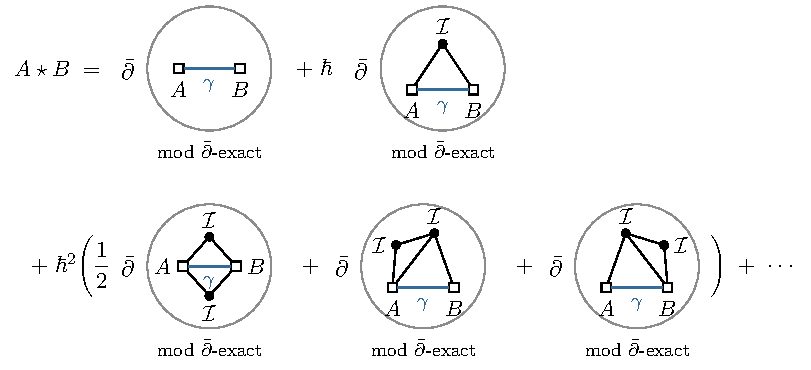
\includegraphics[width=0.86\linewidth]{figures/vec/figures-circuits-product_graphs.pdf}
\caption{The quantum product \eqref{b-00504} through order $\hbar^2$: the free differential $\bar\partial$ acting on the marked graphs, as in \eqref{eq-1-7}. Squares are the insertions $A$ and $B$, dots the interaction vertices $\mathcal I$. The blue edge $\gamma$ is the propagator of the pair $a,b_{\mathrm{aux}}$ in \eqref{eq-2-31}, which acts as the integration contour of \eqref{eq-normal-ordering-theorem}; at order zero $\bar\partial$ turns it into the heat kernel and gives $AB$ \eqref{b-00504}. Black edges contract fields of $\mathcal I$, $A$ and $B$. Each coefficient is $\hbar^n/n!$ times the number of labellings of the interaction vertices.}
\label{fig-product-graphs}
\end{figure}

\rthm{Theorem}{local-7173c1bc-746f-41a1-b0c1-2796d8fbad48}{Leibniz rule}

\emph{Suppose that the interaction satisfies \eqref{eq-2-40}, which is the quantum master equation. (Explicitly, it is the gauge anomaly cancellation condition.)} \emph{For operators $X,Y$, with $|X|$ the fermion number of $X$,\footnote{Equation \eqref{eq-quadratic-two} is the quadratic identity of the higher brackets \cite[Section 3.2]{operatope}, \cite[Theorem 7]{Wang}, \cite[Equation (4.19)]{higher}: in its first three terms the inner bracket contains both $X$ and $Y$, only $X$, and only $Y$, and the terms whose inner bracket contains interactions alone cancel by \eqref{eq-2-40}.}}
\begin{equation}\label{eq-2-52}
\mathbf Q\{X,Y\}_{\mathcal I}
-\{\mathbf QX,Y\}_{\mathcal I}
+(-1)^{|X|}\{X,\mathbf QY\}_{\mathcal I}=0,
\end{equation}
\emph{and the quantum product obeys}
\begin{equation}\label{eq-chain}
\mathbf Q(A\star B)
=(\mathbf QA)\star B+(-1)^{|A|}A\star(\mathbf QB).
\end{equation}

\emph{In particular, quantum multiplication takes quantum cocycles to quantum cocycles and descends to $\mathbf Q$-cohomology.}

\emph{Proof.} For $N\ge1$ interaction entries and the entries $X,Y$, the quadratic identity of the higher brackets \cite[Section 3.2]{operatope}, \cite[Theorem 7]{Wang}, \cite[Equation (4.19)]{higher}, in the conventions of \eqref{eq-2-46}, sorts its terms by the content of the inner bracket:
\begin{equation}\label{eq-quadratic-two}
\begin{aligned}
0={}&\underbrace{\sum_{r=0}^{N-1}\binom Nr\{\mathcal I^{\otimes(N-r)},\{\mathcal I^{\otimes r},X,Y\}_0\}_0}_{\text{inner bracket contains }X\text{ and }Y}
-\underbrace{\sum_{r=1}^{N}\binom Nr\{\mathcal I^{\otimes(N-r)},\{\mathcal I^{\otimes r},X\}_0,Y\}_0}_{\text{inner bracket contains }X}\\
&+(-1)^{|X|}\underbrace{\sum_{r=1}^{N}\binom Nr\{\mathcal I^{\otimes(N-r)},X,\{\mathcal I^{\otimes r},Y\}_0\}_0}_{\text{inner bracket contains }Y}
+\underbrace{\sum_{k=2}^{N}\binom Nk\{\mathcal I^{\otimes(N-k)},\{\mathcal I^{\otimes k}\}_0,X,Y\}_0}_{\text{inner bracket contains only interactions}}.
\end{aligned}
\end{equation}

Multiply by $\hbar^{N-1}/N!$ and sum over $N\ge1$. Since $\binom Nr/N!=1/(r!\,(N-r)!)$, each double sum factorizes into an outer series in $s=N-r$ and an inner series:
\begin{equation}\label{eq-quadratic-two-summed}
\begin{aligned}
0={}&\underbrace{\sum_{s\ge1}\frac{\hbar^{s-1}}{s!}\Big\{\mathcal I^{\otimes s},\sum_{r\ge0}\frac{\hbar^r}{r!}\{\mathcal I^{\otimes r},X,Y\}_0\Big\}_0}_{\mathbf Q\{X,Y\}_{\mathcal I}}
-\underbrace{\sum_{s\ge0}\frac{\hbar^{s}}{s!}\Big\{\mathcal I^{\otimes s},\sum_{r\ge1}\frac{\hbar^{r-1}}{r!}\{\mathcal I^{\otimes r},X\}_0,Y\Big\}_0}_{\{\mathbf QX,Y\}_{\mathcal I}}\\
&+(-1)^{|X|}\underbrace{\sum_{s\ge0}\frac{\hbar^{s}}{s!}\Big\{\mathcal I^{\otimes s},X,\sum_{r\ge1}\frac{\hbar^{r-1}}{r!}\{\mathcal I^{\otimes r},Y\}_0\Big\}_0}_{\{X,\mathbf QY\}_{\mathcal I}}\\
&+\underbrace{\sum_{s\ge0}\frac{\hbar^{s+1}}{s!}\Big\{\mathcal I^{\otimes s},\sum_{k\ge2}\frac{\hbar^{k-2}}{k!}\{\mathcal I^{\otimes k}\}_0,X,Y\Big\}_0}_{0\text{ by \eqref{eq-2-40}}}.
\end{aligned}
\end{equation}

The inner series are \eqref{eq-2-51} and the left side of \eqref{eq-2-40}; this is \eqref{eq-2-52}. The Jacobi identity expresses the Leibniz rule for an adjoint action on a bracket, and \eqref{eq-2-52} is its higher $L_\infty$ form, with the interaction insertions supplying every perturbative order \cite[Sections 4.3--4.5]{higher}.

Set $X=Aa$ and $Y=b_{\mathrm{aux}}B$ in \eqref{eq-2-52}, and extract the auxiliary contraction:
\begin{equation*}
0=\mathbf Q(A\star B)
-(\mathbf QA)\star B-(-1)^{|A|}A\star(\mathbf QB).
\end{equation*}

Consequently, $\mathbf QA=\mathbf QB=0$ gives $\mathbf Q(A\star B)=0$. For homogeneous $X,Y$ with $|X|=|A|+1$ and $|Y|=|B|+1$, the same identity and $\mathbf Q^2=0$ (Lemma~\ref{b-00452}) give
\begin{equation}\label{eq-representatives}
\begin{aligned}
&(A+\mathbf QX)\star(B+\mathbf QY)-A\star B\\
&\qquad=\mathbf Q\bigl(X\star B+(-1)^{|A|}A\star Y
+X\star\mathbf QY\bigr).
\end{aligned}
\end{equation}

The resulting cohomology class is therefore independent of representatives.~\hfill\qedsymbol

\subsection{The quantum BPS ring}\label{sec-ring}

Write $[\cdot]_{\mathbf Q}$ for the class of a quantum cocycle.

\rthm{Theorem}{b-00513}{} \emph{Suppose the interaction satisfies \eqref{eq-2-40}, the quantum master equation. } \emph{The quantum product \eqref{b-00504} induces an associative, graded-commutative, unital multiplication on $H(\mathbf Q)$. } \emph{For quantum cocycles $A,B,D$,}
\begin{equation}\label{eq-ring-associativity}
[(A\star B)\star D]_{\mathbf Q}
=[A\star(B\star D)]_{\mathbf Q},
\end{equation}
\begin{equation}\label{eq-ring-commutativity}
[A\star B]_{\mathbf Q}
=(-1)^{|A||B|}[B\star A]_{\mathbf Q}.
\end{equation}

\emph{The unit is strict:}
\begin{equation}\label{eq-ring-unit}
A\star1=1\star A=A.
\end{equation}

\emph{In the successive homotopy transfer of Section~\ref{sec-homotopy-transfer}, the quantum product induces on every page $E_r$ the ordinary product of leading representatives, and every $d_r$ is a derivation of it.}

\emph{Proof.} The chain identity \eqref{eq-chain} makes the product well-defined on cohomology. A class of $E_r$ has a representative $a+\hbar a_1+\cdots$ whose $\mathbf Q$-variation starts at order $\hbar^r$ with $d_ra$. Since $A\star B=AB+O(\hbar)$, the product of two such representatives has leading term $ab$, and by \eqref{eq-chain} its $\mathbf Q$-variation starts at order $\hbar^r$ with $(d_ra)b+(-1)^{|a|}a\,d_rb$. For the unit, the identity insertion has no fields, so in a marked circuit with $n\ge1$ interaction nodes it is wired only by the marked resistor. It is a dead end: the marked resistor carries the current injected at the identity insertion, whatever its resistance, so this resistance moves no current and the current form vanishes. So only the zero-interaction marked segment contributes.

For three closed insertions $X,Y,Z$, sum the quadratic identities with all interaction entries, as in \cite[Sections 4.3 and 4.5]{higher}. The pure-interaction terms vanish by \eqref{eq-2-40}, and the single-input terms vanish by closure. With the ordered-bracket sign of \eqref{eq-A-28}, the remaining identity is
\begin{equation}\label{eq-ring-twisted-jacobi}
\begin{aligned}
0={}&\{X,\{Y,Z\}_{\mathcal I}\}_{\mathcal I}
-\{\{X,Y\}_{\mathcal I},Z\}_{\mathcal I}\\
&-(-1)^{(|X|+1)(|Y|+1)}
\{Y,\{X,Z\}_{\mathcal I}\}_{\mathcal I}\\
&+\mathbf Q\sum_{n\ge0}\frac{\hbar^{n+1}}{n!}
\{\mathcal I^{\otimes n},X,Y,Z\}_0.
\end{aligned}
\end{equation}

A ternary graph with $n$ interactions has $n+3$ vertices and $2n+3$ edges, hence loop number $n+1$. This fixes the power of $\hbar$ in the last line.

Take two independent copies $(a_1,b_{\mathrm{aux},1})$ and $(a_2,b_{\mathrm{aux},2})$ of the free auxiliary pair defined above. Each $a_i$ is even and each $b_{\mathrm{aux},i}$ is odd. Substitute
\begin{equation*}
X=Aa_1,\qquad Y=Da_2,\qquad
Z=b_{\mathrm{aux},1}b_{\mathrm{aux},2}B.
\end{equation*}

The last insertion is the root. This marks the edges $AB$ and $DB$, as in Figure~\ref{b-00530}.

\begin{figure}[H]
\centering
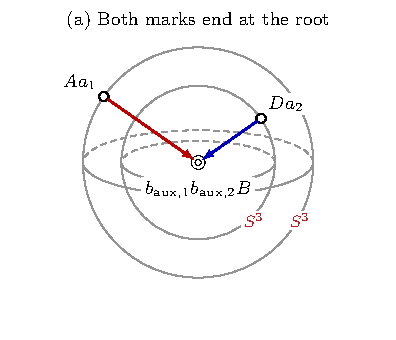
\includegraphics[width=0.47\linewidth]{figures/vec/fig11-integration-spheres-a-20261102.pdf}\hfill
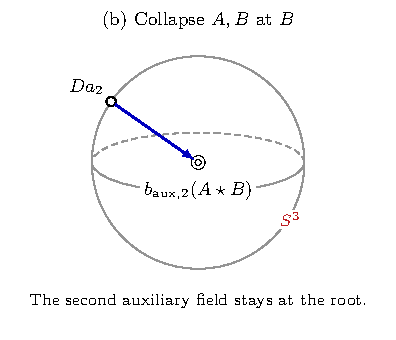
\includegraphics[width=0.47\linewidth]{figures/vec/fig11-integration-spheres-b-20261102.pdf}\\[4pt]
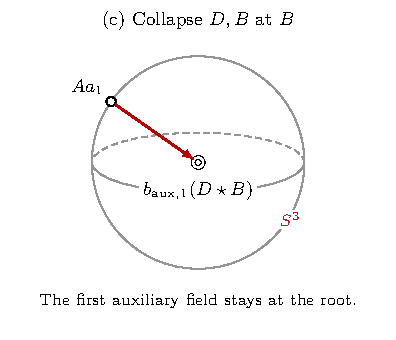
\includegraphics[width=0.47\linewidth]{figures/vec/fig11-integration-spheres-c-20261102.pdf}\hfill
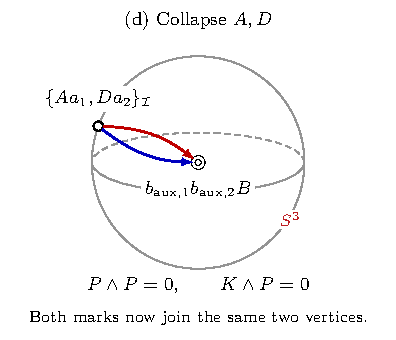
\includegraphics[width=0.47\linewidth]{figures/vec/fig11-integration-spheres-d-20261102.pdf}
\caption{The common-root contraction and its three pair-collapse channels. Red and blue arrows mark the first and second auxiliary pairs; double circles mark the root. Each non-root insertion lies on its own integration sphere $S^3$ centered at the root, shown schematically in gray. Only auxiliary contractions are shown. Each component may also contain interaction vertices and physical contractions. The labels in (b) and (c) display the surviving fields; their Koszul signs are given in the proof.}
\label{b-00527}
\label{b-00528}
\label{b-00529}
\label{b-00530}
\end{figure}

The ordered-bracket sign gives
\begin{equation}\label{eq-ring-root-contractions}
\begin{aligned}
\left.\{Aa_1,b_{\mathrm{aux},1}b_{\mathrm{aux},2}B\}_{\mathcal I}
\right|_{a_1=b_{\mathrm{aux},1}=0}
&=(-1)^{|A|}b_{\mathrm{aux},2}(A\star B),\\
\left.\{Da_2,b_{\mathrm{aux},1}b_{\mathrm{aux},2}B\}_{\mathcal I}
\right|_{a_2=b_{\mathrm{aux},2}=0}
&=(-1)^{|D|+1}b_{\mathrm{aux},1}(D\star B).
\end{aligned}
\end{equation}

In the second line the odd derivative passes through $b_{\mathrm{aux},1}$, contributing the extra minus sign.

The third binary channel first collapses $A,D$. Both marked resistors then join that collapsed node to $B$: they are in parallel, and their proportional currents kill the measure for every holomorphic derivative (Corollary~\ref{b-00188}, \eqref{eq-1-13}). Consequently,
\begin{equation}\label{eq-ring-parallel-channel}
\left.
\{\{Aa_1,Da_2\}_{\mathcal I},
b_{\mathrm{aux},1}b_{\mathrm{aux},2}B\}_{\mathcal I}
\right|_{\mathrm{aux}=0}=0.
\end{equation}

On substituting \eqref{eq-ring-root-contractions} and \eqref{eq-ring-parallel-channel} into \eqref{eq-ring-twisted-jacobi}, each of its three nested brackets becomes a product of three operators:
\begin{equation}\label{eq-ring-twisted-jacobi-substituted}
0=\underbrace{(-1)^{|D|+1}A\star(D\star B)}_{\{X,\{Y,Z\}_{\mathcal I}\}_{\mathcal I}}
-\underbrace{0}_{\substack{\{\{X,Y\}_{\mathcal I},Z\}_{\mathcal I}:\\\text{parallel marks}}}
\underbrace{-(-1)^{(|A|+1)(|D|+1)+|A|}D\star(A\star B)}_{-(-1)^{(|X|+1)(|Y|+1)}\{Y,\{X,Z\}_{\mathcal I}\}_{\mathcal I}}
+\underbrace{\mathbf Q\,H}_{\mathbf Q\text{-exact}},
\end{equation}
with $H$ the bracket in the last line of \eqref{eq-ring-twisted-jacobi} at these inputs. The middle term vanishes, so only the two bracketings $A\star(D\star B)$ and $D\star(A\star B)$ remain. Multiplying by $(-1)^{|D|+1}$ gives the local homotopy
\begin{equation}\label{eq-ring-common-root-homotopy}
\begin{aligned}
&A\star(D\star B)-(-1)^{|A||D|}D\star(A\star B)\\
&\quad=(-1)^{|D|}\mathbf Q
\left[
\left.\sum_{n\ge0}\frac{\hbar^{n+1}}{n!}
\{\mathcal I^{\otimes n},Aa_1,Da_2,
 b_{\mathrm{aux},1}b_{\mathrm{aux},2}B\}_0
\right|_{\mathrm{aux}=0}\right].
\end{aligned}
\end{equation}

Moreover, its $n$-interaction term has $2n+1$ physical contractions. The interactions supply at most $n$ fields of type $\mathsf b$ or $\beta$, so at least $n+1$ must come from the inputs. The homotopy is therefore a finite sum of local operators for finite polynomial inputs.

Setting $B=1$ proves graded commutativity. For three closed inputs, \eqref{eq-chain}, graded commutativity, and \eqref{eq-ring-common-root-homotopy} give
\begin{equation}\label{eq-ring-associativity-proof}
\begin{aligned}
[(A\star B)\star D]_{\mathbf Q}
&\underset{\eqref{eq-ring-commutativity}}{=}(-1)^{(|A|+|B|)|D|}[D\star(A\star B)]_{\mathbf Q}\\
&\underset{\eqref{eq-ring-common-root-homotopy}}{=}(-1)^{|B||D|}[A\star(D\star B)]_{\mathbf Q}\\
&\underset{\eqref{eq-ring-commutativity}}{=}[A\star(B\star D)]_{\mathbf Q}.
\end{aligned}
\end{equation}

The $\mathbf Q$-exact term of \eqref{eq-ring-common-root-homotopy} drops out of the classes; this is the potential $\mathbf Q$-exact difference between the two bracketings in \eqref{eq-ring-associativity}. This proves the stated ring laws.~\hfill\qedsymbol

\subsection{The graph formula of the quantum product}\label{the-graph-formula}

For a physical edge $(v,w)$, the operator $\Delta_{vw}$ contracts one field at vertex $v$ with its BV conjugate at vertex $w$, using the pairing~\eqref{eq-A-20}. For example, in the $\mathcal N=4$ superfield variables, at fixed vertex positions,
\begin{equation*}
\Delta_{vw}=-\delta^{DE}\int d^3\theta\,
\frac{\delta}{\delta C_v^D(\theta)}
\frac{\delta}{\delta C_w^E(\theta)}.
\end{equation*}

Here $C_v^D$ is the field at vertex $v$, and the fibre derivatives are given by~\eqref{eq-A-16}. Composing these contractions in edge order gives the graph coefficient
\begin{equation}\label{eq-2-31}
\begin{aligned}
\frac1{n!}\{\mathcal I^{\otimes n},A,B\}^{\gamma,0}
={}&\left.\frac1{n!}\{\mathcal I^{\otimes n},Aa,b_{\mathrm{aux}}B\}_0\right|_{\mathrm{aux}=0}\\
={}&\frac{(-1)^n}{n!(8\pi^2)^n}
\sum_{\substack{\Gamma\ \mathrm{labelled,\ Laman}\\
|V|=n+2,\ |I|=2n+1\\(n+1,n+2)\in I}}
\Bigg[\mathcal I_\Gamma(\lambda;z)\\
&\qquad\times\prod_{(v,w)\in I\setminus\{(n+1,n+2)\}}^{\mathrm{edge\ order}}
\Delta_{vw}(\mathcal I_1\cdots\mathcal I_nA_{n+1}B_{n+2})\Bigg]_{\mathrm{jets},\,x_v=x,\,z=0}.
\end{aligned}
\end{equation}

Here $\gamma=\{(n+1,n+2)\}$, with $\mathrm{aux}=0$ imposed after contraction.

In the subscript $\mathrm{jets}$, each derivative on a contracted input field differentiates the kernel through its edge displacement, while $\lambda_v$ differentiates the surviving fields at vertex $v$.

The displacements are then set to zero and all vertex positions to the common insertion point $x$. The graph restrictions of Section~\ref{sec-forests} reduce this sum to product forests.

\rthm{Corollary}{local-ch8-finite-product-corollary}{Finiteness of the quantum product}

For polynomial local inputs and a polynomial superpotential in the interaction \eqref{eq-B-10}, the quantum product has finitely many powers of $\hbar$.

\emph{Proof.} Each order-$n$ product graph has $n$ interaction vertices and $2n$ physical contractions, so Proposition \ref{b-00249} gives
\begin{equation*}
\begin{aligned}
\#(\mathsf b,\beta\text{ in output})
&=\#(\mathsf b,\beta\text{ in }A)+\#(\mathsf b,\beta\text{ in }B)\\
&\quad+\underbrace{n-\#(\bar W\text{ vertices})}_{\text{interaction terminals}}
-\underbrace{2n}_{\text{physical contractions}}\\
&=\#(\mathsf b,\beta\text{ in }A)+\#(\mathsf b,\beta\text{ in }B)-n-\#(\bar W\text{ vertices})\ge0.
\end{aligned}
\end{equation*}

Writing $[\hbar^n]$ for the coefficient of $\hbar^n$, we obtain
\begin{equation}\label{local-ch8-finite-product-bound}
[\hbar^n](A\star B)=0
\quad\text{if}\quad
n>\#(\mathsf b,\beta\text{ in }A)+\#(\mathsf b,\beta\text{ in }B).
\end{equation}

For polynomial inputs the counts are the maxima over their monomials; the same loss adds at the binary vertices of any fixed bracketing of finitely many inputs.

For a formal superpotential the bound holds coefficientwise in its coefficients. $\square$

\subsection{One- and two-loop examples in $\mathcal N=4$ Yang--Mills theory}\label{sec-product-loops}

The one-loop triangle has vertices $1:\mathcal I$, $2:A$ and $3:B$, and marked edge $\gamma=\{(2,3)\}$. Its kernel is exactly the same as the fan kernel. Pairing its displacement exponential with the spatial functional derivatives of \eqref{eq-2-10} gives
\begin{equation}\label{eq-2-34}
\begin{aligned}
\{\mathcal I,A,B\}^{\{(2,3)\},0}(x)
={}&\frac{i}{32\pi^2}\int_0^1dr_1\int_0^{1-r_1}dr_2
\int d^3\theta\,C_{XYZ}\\
&\times\int d^4z_1\,d^4z_2\\
&\times(\partial_{+\dot a}C^X)
\big(x+r_1z_1+(1-r_1)z_2,\theta\big)\\
&\times\left.
\partial_{2,+}{}^{\dot a}
\left(\frac{\delta A(x_2)}{\delta C^Y(x_2+z_1,\theta)}\right)
\right|_{x_2=x+r_2(z_2-z_1)}
\frac{\delta B(x)}{\delta C^Z(x+z_2,\theta)}.
\end{aligned}
\end{equation}

Here $x$ is the arbitrary common position of the local product.

At two loops the physical graphs have four edges (plus, as always, one edge for the auxiliary fields). They consist of a book and two triangles attached to opposite inputs (Figure~\ref{fig-two-loop-product}). Their ordered edges, for $3=A$ and $4=B$, are
\begin{equation}\label{eq-productedges}
\begin{aligned}
\Gamma_{\mathrm{book}}&:(13,14,23,24,34),\\
\Gamma_A&:(12,13,23,24,34),\\
\Gamma_B&:(12,14,23,24,34).
\end{aligned}
\end{equation}

\begin{figure}[H]
\centering
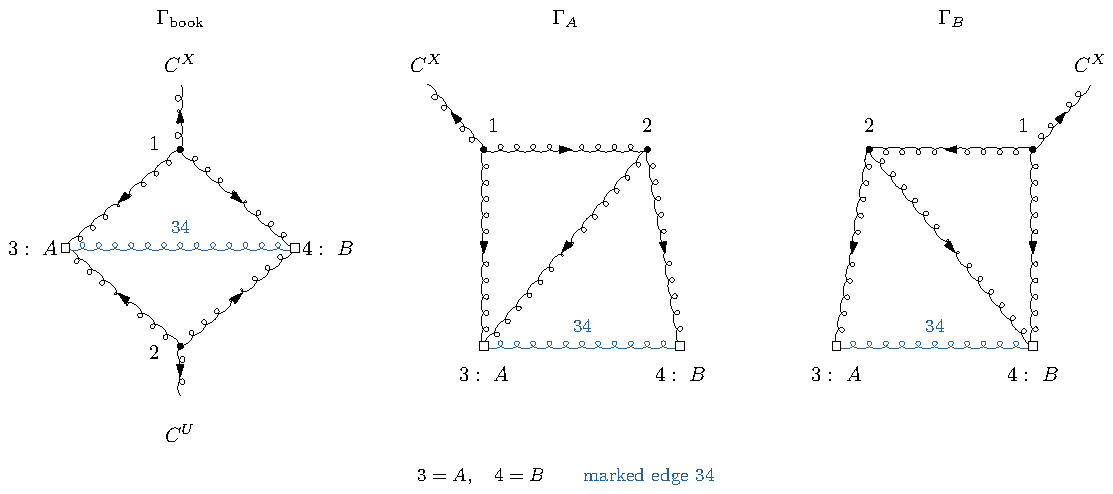
\includegraphics[width=0.96\linewidth]{figures/vec/figures-two_loop_product_feynarts.pdf}
\caption{The two-loop quantum-product graphs $\Gamma_{\mathrm{book}}$, $\Gamma_A$ and $\Gamma_B$. Squares are the insertions $3:A$ and $4:B$; dots are cubic interactions. Black arrows orient the physical contractions, and the blue edge $(3,4)$ carries the auxiliary pairing. The book leaves $C^X,C^U$ uncontracted; each triangle leaves $C^X$.}
\label{fig-two-loop-product}
\end{figure}

The last edge is the auxiliary edge. These are still fan kernels (but with more free injected momenta).
\begin{equation}\label{eq-productkernels}
\begin{aligned}
\mathcal I_{\Gamma_{\mathrm{book}}}(\lambda;0)
&=\frac1{24}
\big[\lambda_{1,+\dot a}(\lambda_{2,+}{}^{\dot a}+2\lambda_{3,+}{}^{\dot a})\big]
\big[\lambda_{2,+\dot b}(\lambda_{1,+}{}^{\dot b}+2\lambda_{3,+}{}^{\dot b})\big],\\
\mathcal I_{\Gamma_A}(\lambda;0)
&=-\frac1{24}(\lambda_{1,+\dot a}\lambda_{3,+}{}^{\dot a})^2,\\
\mathcal I_{\Gamma_B}(\lambda;0)
&=\frac1{24}(\lambda_{1,+\dot a}\lambda_{3,+}{}^{\dot a})^2.
\end{aligned}
\end{equation}

For the full result, the book kernel gives
{\small
\begin{equation}\label{eq-product2book}
\begin{aligned}
&\left.\frac12\{\mathcal I,\mathcal I,A,B\}^{\gamma,0}(x)\right|_{\Gamma_{\mathrm{book}}}\\
&\quad=\frac{C_{XYZ}C_{UVW}}{2(32\pi^2)^2}
\int_0^1dr_1\int_0^1dr_3\int_0^1dr_2\int_0^{1-r_2}dr_4\,
(1-r_2-r_4)\\
&\times\int d^3\theta^{(1)}d^3\theta^{(2)}\,
\int\prod_{e\in\{13,14,23,24\}}d^4z_e\\
&\times\partial_{1,+\dot a}
(\partial_{3,+}{}^{\dot a}+r_3\partial_{2,+}{}^{\dot a})
\partial_{2,+\dot b}
(\partial_{3,+}{}^{\dot b}+r_1\partial_{1,+}{}^{\dot b})\\
&\times\Bigg[
C^X(x_1,\theta^{(1)})C^U(x_2,\theta^{(2)})\\
&\qquad\times
\frac{\delta^2A(x_3)}{
\delta C^Y(x_3+z_{13},\theta^{(1)})
\delta C^V(x_3+z_{23},\theta^{(2)})}
\frac{\delta^2B(x)}{
\delta C^Z(x+z_{14},\theta^{(1)})
\delta C^W(x+z_{24},\theta^{(2)})}
\Bigg]_{x_v=x_v(x;r,z),\,v=1,2,3} .
\end{aligned}
\end{equation}
}

The translated positions are
\begin{equation*}
\begin{aligned}
x_1(x;r,z)&=x+r_1z_{13}+(1-r_1)z_{14}
+r_1\big[r_2(z_{14}-z_{13})+r_4(z_{24}-z_{23})\big],\\
x_2(x;r,z)&=x+r_3z_{23}+(1-r_3)z_{24}
+r_3\big[r_2(z_{14}-z_{13})+r_4(z_{24}-z_{23})\big],\\
x_3(x;r,z)&=x+r_2(z_{14}-z_{13})+r_4(z_{24}-z_{23}).
\end{aligned}
\end{equation*}

For $\Gamma_A$, the translated positions are
\begin{equation*}
\begin{aligned}
x_1^{+\dot a}(x;r,z)
={}&x^{+\dot a}+\big[r_1r_2+(1-r_2)(r_1r_3+r_4)\big]z_{13}^{+\dot a}
-r_2\big[r_1(1-r_3)-r_4\big]z_{23}^{+\dot a}\\
&+(1-r_1r_3-r_4)z_{24}^{+\dot a},\\
x_3^{+\dot a}(x;r,z)
={}&x^{+\dot a}+(1-r_3-r_4)
\big[z_{24}^{+\dot a}-(1-r_2)z_{13}^{+\dot a}-r_2z_{23}^{+\dot a}\big].
\end{aligned}
\end{equation*}

The full contribution is
\begin{equation}\label{eq-product2A}
\begin{aligned}
&\left.\frac12\{\mathcal I,\mathcal I,A,B\}^{\gamma,0}(x)\right|_{\Gamma_A}\\
&\quad=\frac{C_{XYR}C_{RZW}}{(32\pi^2)^2}
\int_0^1dr_1\int_0^1dr_2\int_0^1dr_3\int_0^{1-r_3}dr_4\\
&\times r_2(1-r_1)(1-r_3-r_4)
\int d^3\theta\,
\int\prod_{e\in\{13,23,24\}}d^4z_e\\
&\times(\partial_{+\dot a}\partial_{+\dot b}C^X)
\big(x_1(x;r,z),\theta\big)\\
&\times\left.
\partial_{3,+}{}^{\dot a}\partial_{3,+}{}^{\dot b}
\left(
\frac{\delta^2 A(x_3)}{
\delta C^Y(x_3+z_{13},\theta)\,
\delta C^Z(x_3+z_{23},\theta)}
\right)\right|_{x_3=x_3(x;r,z)}
\frac{\delta B(x)}{\delta C^W(x+z_{24},\theta)}.
\end{aligned}
\end{equation}

For $\Gamma_B$, the translated positions are
\begin{equation*}
\begin{aligned}
x_1^{+\dot a}(x;r,z)
={}&x^{+\dot a}+\big[1-r_1r_2-r_1(1-r_2)r_3\big]z_{14}^{+\dot a}
+r_1r_3z_{23}^{+\dot a}
+r_1r_2(1-r_3)z_{24}^{+\dot a},\\
x_3^{+\dot a}(x;r,z)
={}&x^{+\dot a}+r_4\big[(1-r_2)z_{14}^{+\dot a}-z_{23}^{+\dot a}
+r_2z_{24}^{+\dot a}\big].
\end{aligned}
\end{equation*}

Thus
\begin{equation}\label{eq-product2B}
\begin{aligned}
&\left.\frac12\{\mathcal I,\mathcal I,A,B\}^{\gamma,0}(x)\right|_{\Gamma_B}\\
&\quad=-\frac{C_{XZR}C_{RYW}}{(32\pi^2)^2}
\int_0^1dr_1\int_0^1dr_2\int_0^1dr_3\int_0^{1-r_3}dr_4\\
&\times r_1r_2r_4\int d^3\theta\,
\int\prod_{e\in\{14,23,24\}}d^4z_e\\
&\times(\partial_{+\dot a}\partial_{+\dot b}C^X)
\big(x_1(x;r,z),\theta\big)\\
&\times\left.
\partial_{3,+}{}^{\dot a}\partial_{3,+}{}^{\dot b}
\left(\frac{\delta A(x_3)}{\delta C^Y(x_3+z_{23},\theta)}\right)
\right|_{x_3=x_3(x;r,z)}
\frac{\delta^2 B(x)}{
\delta C^Z(x+z_{14},\theta)\,\delta C^W(x+z_{24},\theta)}.
\end{aligned}
\end{equation}

The exchange $3\leftrightarrow4$ maps $\Gamma_A$ to $\Gamma_B$: after restoring the displayed edge order, $\mathcal I_{\Gamma_B}(\lambda;0)=-\mathcal I_{\Gamma_A}(\lambda;0)$ in \eqref{eq-productkernels}; the full displaced formulas also require exchanging the inputs, their edge displacements, and the root.

\subsection{Order-by-order representatives}\label{sec-order-by-order}

For $Q_0A=Q_0B=0$, the first two orders of \eqref{eq-chain} are
\begin{equation}\label{eq-2-55}
\begin{aligned}
Q_0\{\mathcal I,A,B\}^{\gamma,0}+Q_1(AB)
={}&(Q_1A)B+(-1)^{|A|}A(Q_1B),\\[3pt]
\frac12Q_0\{\mathcal I,\mathcal I,A,B\}^{\gamma,0}
+Q_1\{\mathcal I,A,B\}^{\gamma,0}+Q_2(AB)
={}&(Q_2A)B+(-1)^{|A|}A(Q_2B)\\
&+\{\mathcal I,Q_1A,B\}^{\gamma,0}
+(-1)^{|A|}\{\mathcal I,A,Q_1B\}^{\gamma,0}.
\end{aligned}
\end{equation}

Thus, the classical variation of the one-loop term of the quantum product cancels the one-loop cross-contraction. Its two-loop term absorbs the remaining two-loop defect together with the action of $Q_1$ on the one-loop term.

If $A=\sum_i\hbar^iA_i$ and $B=\sum_j\hbar^jB_j$ are quantum cocycles, their product has coefficients
\begin{equation}\label{eq-2-32}
\mathcal O_r=\sum_{i+j+n=r}\frac1{n!}\{\mathcal I^{\otimes n},A_i,B_j\}^{\gamma,0},\qquad\mathcal O_0=A_0B_0\ \text{\eqref{b-00504}},
\end{equation}
\begin{equation}\label{eq-2-33}
\begin{aligned}
\mathcal O_1={}&A_1B_0+A_0B_1
+{\{\mathcal I,A_0,B_0\}^{\gamma,0}},\\
\mathcal O_2={}&A_2B_0+A_1B_1+A_0B_2\\
&+\{\mathcal I,A_1,B_0\}^{\gamma,0}
+\{\mathcal I,A_0,B_1\}^{\gamma,0}
+{\frac12\{\mathcal I,\mathcal I,A_0,B_0\}^{\gamma,0}}.
\end{aligned}
\end{equation}

Equation~\eqref{eq-chain} gives $\sum_{k=0}^rQ_k\mathcal O_{r-k}=0$ at every order. These are the lifting equations \eqref{eq-liftingequations} for the product $A_0B_0$: the quantum product gives in closed form the completion that the homotopy transfer of Section~\ref{sec-homotopy-transfer} constructs order by order.

\subsection{Normal ordering and an explicit associator}\label{sec-normal-ordering}

\paragraph{Normal ordering.}\label{quantum-normal-ordering}

The quantum normal-ordering product is represented by the Bochner--Martinelli contour \eqref{eq-normal-ordering-theorem} \cite[Section 2.3]{semichiral}.

We now prove that it agrees, up to exact terms, with the quantum product of Sections~\ref{sec-dressed-chain}--\ref{sec-order-by-order}.

Here $(A(x)B(0))[L]$ denotes the joint renormalized two-insertion expansion at scale $L$, defined for local insertions $X$ by $X[L]\,e^{I[L]/\hbar}=\lim_{\varepsilon\downarrow0}e^{\hbar\partial_{P_{\varepsilon,L}}}\bigl(X\,e^{I/\hbar}\bigr)$ with $I=\int_{\mathbb C^2}\Omega\wedge[\mathcal I]_{(0,2)}$ \cite{Costello}. (The scale $L$ belongs to Costello's formalism of BV renormalization theory; it never affects our calculations.)

The contour argument uses renormalized separated insertions satisfying the supersymmetry descent Ward identity \cite[Sections 2.2--2.3]{semichiral}.

Let $A(x,\bar\theta)[L]$ be the renormalized supersymmetry multiplet of the effective insertion $A[L]$. In the coordinates of \eqref{eq-B-7},
\begin{equation}\label{eq-ring-descendant}
\begin{aligned}
A^{(1)}(x)[L]
&=\frac14dx^{-\dot a}
\left.\frac{\partial_L A(x,\bar\theta)[L]}{\partial\bar\theta^{\dot a}}
\right|_{\bar\theta=0},\\
\bigl(\bar\partial+(I[L],\,\cdot\,)_L+\hbar\Delta_L\bigr)
A^{(1)}[L]+\bar\partial_x A[L]&=(\mathbf QA)^{(1)}[L].
\end{aligned}
\end{equation}

Taking the one-form component of the full composite multiplet gives its descendant \cite[Section 2.2]{semichiral}.

\begin{proofbox}
For $\mathbf QA=0$, write the form to the left of its coefficient:
\begin{equation}\label{eq-ring-descendant-component}
\begin{aligned}
A^{(1)}[L]&=dx^{-\dot a}A^{(1)}_{-\dot a}[L],\\
\frac{\partial A[L]}{\partial x^{-\dot a}}
&=\bigl(\bar\partial+(I[L],\,\cdot\,)_L+\hbar\Delta_L\bigr)
A^{(1)}_{-\dot a}[L].
\end{aligned}
\end{equation}

This gives the primitive of an antiholomorphic translation in the effective-observable complex.
\end{proofbox}

At zero displacement, \eqref{eq-C-explicit-propagator} gives
\begin{equation}\label{eq-ring-propagator-residue}
\begin{gathered}
[P_{0,\infty}(x)]_\Omega
=-\frac{x^-_{\dot a}dx^{-\dot a}}
{8\pi^2|x|_E^4},\qquad
d\bigl(\Omega\wedge[P_{0,\infty}]_\Omega\bigr)
=\delta_E^{(4)}(x)d^4x_E,\\
\int_{S^3}\Omega\wedge[P_{0,\infty}]_\Omega=1.
\end{gathered}
\end{equation}

The last integral holds for every positively oriented embedded three-sphere enclosing the origin once; its normalization is that of the heat kernel,
\begin{equation*}
\int_{|x|_E\le r}\Omega\wedge[K_\varepsilon]_\Omega
=1-\left(1+\frac{r^2}{2\varepsilon}\right)e^{-r^2/(2\varepsilon)}
\xrightarrow{\varepsilon\downarrow0}1.
\end{equation*}

Let $(A(x)B(0))^{(1)}[L]$ be the first descendant of the joint insertion with respect to the position $x$.

For closed inputs and $S_1^3-S_0^3=\partial V$, with $V$ disjoint from all insertions,
\begin{equation}\label{eq-ring-sphere-homotopy}
\begin{aligned}
&\int_{S_1^3}\Omega\wedge[P_{0,\infty}]_\Omega(A(x)B(0))[L]
-\int_{S_0^3}\Omega\wedge[P_{0,\infty}]_\Omega(A(x)B(0))[L]\\
&\quad=-\bigl(\bar\partial+(I[L],\,\cdot\,)_L+\hbar\Delta_L\bigr)
\int_V\Omega\wedge[P_{0,\infty}]_\Omega
\wedge(A(x)B(0))^{(1)}[L].
\end{aligned}
\end{equation}

For $\mathbf QA=\mathbf QB=0$, descent gives $\bar\partial_x(A(x)B(0))[L]=-\bigl(\bar\partial+(I[L],\,\cdot\,)_L+\hbar\Delta_L\bigr)(A(x)B(0))^{(1)}[L]$; the propagator is closed on $V$, so

\begin{equation*}
\begin{aligned}
\int_{\partial V}\Omega\wedge[P_{0,\infty}]_\Omega(A(x)B(0))[L]
&=-\int_V\Omega\wedge[P_{0,\infty}]_\Omega\wedge\bar\partial_x(A(x)B(0))[L]\\
&=-\bigl(\bar\partial+(I[L],\,\cdot\,)_L+\hbar\Delta_L\bigr)
\int_V\Omega\wedge[P_{0,\infty}]_\Omega\wedge(A(x)B(0))^{(1)}[L].
\end{aligned}
\end{equation*}

Equation~\eqref{eq-ring-sphere-homotopy} proves equality of the contour classes in the effective-observable complex.

\rthm{Theorem}{b-00598}{Normal-ordering comparison} \emph{Let $A$ and $B$ be homogeneous quantum cocycles and $L>0$. } \emph{In the effective-observable complex at scale $L$, with differential $\mathbf Q_L=Q_{\mathrm{BV}}+(I[L],\,\cdot\,)_L+\hbar\Delta_L$, let $B_R$ be the ball of radius $R$ centred at the insertion of $B$ and $S_R^3=\partial B_R$. The contour product and the effective representative of \eqref{b-00504} satisfy}
\begin{equation}\label{eq-normal-ordering-theorem}
\begin{aligned}
&\int_{S_R^3}\Omega\wedge[P_{0,\infty}(x)]_\Omega\,(A(x)B(0))[L]\\
&\quad=(A\star B)[L]
-\mathbf Q_L\int_{B_R}\Omega\wedge[P_{0,\infty}(x)]_\Omega
\wedge(A(x)B(0))^{(1)}[L].
\end{aligned}
\end{equation}

\emph{Proof.}

Write $F(x)=(A(x)B(0))[L]$ and $F^{(1)}(x)=(A(x)B(0))^{(1)}[L]$. The volume integral uses the full joint descendant and has type $(2,2)$. Evaluate it as one coefficientwise graph limit in the decoupled auxiliary theory: physical edges carry $P_{\varepsilon,L}$ and the marked edge carries $P_{\varepsilon,\infty}$. Take the limit only after combining the ordered graphs. The marked edge is last, has zero displacement, and its single Wick factor $\hbar$ is divided out.
\begin{equation}\label{eq-normal-ordering-J}
\begin{gathered}
\bar\partial P_{\varepsilon,L}=K_\varepsilon-K_L,
\qquad \bar\partial P_{\varepsilon,\infty}=K_\varepsilon,\\
|V|=n+2,\qquad |I|=2n+1,\qquad
\frac1\hbar\frac{\hbar^{2n+1}}{n!\hbar^n}=\frac{\hbar^n}{n!}.
\end{gathered}
\end{equation}

Apply \eqref{eq-normal-ordering-J} to every edge, with the signs $(-1)^{j-1}$ of \eqref{eq-A-28}. The upper physical-edge faces assemble into $\mathbf Q_L$; pure-interaction collision faces cancel by the quantum master equation, and faces with only one insertion vanish by $\mathbf QA=\mathbf QB=0$. A remaining cluster contains both insertions and $n$ interactions. The rescaling $t_e\mapsto\varepsilon t_e$, $x_v\mapsto\sqrt\varepsilon\,x_v$ sends the physical upper endpoint to $L/\varepsilon\to\infty$, yielding exactly the projective marked kernel \eqref{eq-2-31}. The ordered Wick signs are those of \eqref{eq-A-28}; the zero-interaction identity in \eqref{b-00504} fixes the collision sign to $+AB$.
\begin{equation}\label{eq-normal-ordering-smeared}
\left[
\left.\sum_{n\ge0}\frac{\hbar^n}{n!}
\{\mathcal I^{\otimes n},Aa,b_{\mathrm{aux}}B\}_0
\right|_{\mathrm{aux}=0}
\right][L]
=(A\star B)[L].
\end{equation}

The graphs outside each collapsed cluster reconstruct its effective representative by the Ward identity $\mathbf Q_L(\mathcal O[L])=(\mathbf Q\mathcal O)[L]$ of a local insertion, the zero-form counterpart of \eqref{eq-ring-descendant}. The same ultraviolet-finite holomorphic graph prescription applies to the decoupled auxiliary extension. Away from the collision faces, the closed-input descent identity is $\bar\partial_xF=-\mathbf Q_LF^{(1)}$. The remaining boundary is $S_R^3$. Since $\Omega\wedge[P_{0,\infty}]_\Omega$ has odd degree, the regulated Stokes identity gives
\begin{equation}\label{eq-normal-ordering-stokes}
\begin{aligned}
\mathbf Q_L\int_{B_R}\Omega\wedge[P_{0,\infty}]_\Omega\wedge F^{(1)}
&=-\int_{B_R}\Omega\wedge[P_{0,\infty}]_\Omega\wedge\mathbf Q_LF^{(1)}\\
&=\int_{B_R}\Omega\wedge[P_{0,\infty}]_\Omega\wedge\bar\partial_xF\\
&=(A\star B)[L]-\int_{S_R^3}\Omega\wedge[P_{0,\infty}]_\Omega F.
\end{aligned}
\end{equation}

This is \eqref{eq-normal-ordering-theorem}. The collision coefficient is independent of $L$ by this rescaling \cite[Theorem 6]{Wang}; $L$ remains in the effective representatives and their differential.\hfill\qedsymbol

\paragraph{An explicit associator example.}\label{an-explicit-associator}

\rthm{Example}{b-00610}{} In $\mathcal N=4$ Yang--Mills theory, let $A$ and $B$ be gauge-invariant polynomials in the scalar fields $(\gamma^I)_X$~(a subsector of the BMN sector), without holomorphic derivatives, and set $D=(\gamma^3)_X(\beta_2)^X$. Then
\begin{equation}\label{eq-ring-scalar-associator}
\begin{aligned}
&(A\star B)\star D-A\star(B\star D)\\
&\quad=\mathbf Q\left\{
\frac{\hbar}{64\pi^2}
\left[
(\partial_{+\dot a}B)\partial_+{}^{\dot a}
\frac{\partial A}{\partial(\gamma^2)_X}
+(\partial_{+\dot a}A)\partial_+{}^{\dot a}
\frac{\partial B}{\partial(\gamma^2)_X}
\right](\gamma^3)_X\right\}.
\end{aligned}
\end{equation}

\emph{Proof.} Gauge invariance gives $Q_0A=Q_0B=0$. Since~$C^{XYZ}(\gamma^3)_X(\gamma^3)_Y(\gamma^1)_Z$~is zero, $Q_0 D$ is also zero. The possible one-loop action on $D$ contains $(\theta_1\theta_2)\theta_2=0$, and $Q_{n\ge2}$ requires at least three input fields. Thus $\mathbf QD=0$. Equation~\eqref{eq-2-34} gives
\begin{equation*}
\{\mathcal I,A,D\}^{\gamma,0}
=\frac{g}{64\pi^2}C_{EX}{}^Y
(\partial_{+\dot a}\mathsf c^E)
\partial_+{}^{\dot a}
\left(\frac{\partial A}{\partial(\gamma^2)_X}\right)
(\gamma^3)_Y.
\end{equation*}

Each physical contraction uses one $\mathsf b$ or $\beta$. For an order-$n$ product, the $n$ interactions supply at most $n$ such factors, and $D$ supplies one; its $2n$ physical contractions therefore require $n\le1$~(one-loop exact). Products between operators containing only $\mathsf c$ and $\gamma$ have no quantum correction. Expanding the two bracketings consequently gives, exactly,
\begin{equation*}
\begin{aligned}
&(A\star B)\star D-A\star(B\star D)\\
&\quad=\frac{\hbar g}{64\pi^2}C_{EX}{}^Y
(\partial_{+\dot a}\mathsf c^E)
\left[
\frac{\partial A}{\partial(\gamma^2)_X}
\partial_+{}^{\dot a}B
+(\partial_+{}^{\dot a}A)
\frac{\partial B}{\partial(\gamma^2)_X}
\right](\gamma^3)_Y.
\end{aligned}
\end{equation*}

We have
\begin{equation*}
Q_0\left[
\partial_+{}^{\dot a}\left(
\frac{\partial A}{\partial(\gamma^2)_X}\right)(\gamma^3)_X
\right]
=-gC_{EX}{}^Y(\partial_+{}^{\dot a}\mathsf c^E)
\frac{\partial A}{\partial(\gamma^2)_X}(\gamma^3)_Y.
\end{equation*}

The same identity holds for $B$. Together with the antisymmetry of the dotted-index contraction, it evaluates the displayed $\mathbf Q$-variation to the associator. For an operator containing only $\gamma$ and its derivatives, an $n$-loop supercharge graph would require $2n+1\le n+1$, so all its positive-loop variations vanish. This also gives $\mathbf QA=\mathbf QB=0$ and shows that no further terms enter the primitive.~\hfill\qedsymbol

For example, take $A=B=\delta^{XY}(\gamma^2)_X(\gamma^2)_Y$. The two gradient terms coincide, and the formula becomes
\begin{equation}\label{eq-ring-explicit-associator}
\begin{aligned}
&(A\star B)\star D-A\star(B\star D)\\
&\quad=\frac{\hbar g}{16\pi^2}C_E{}^{XY}
(\partial_{+\dot a}\mathsf c^E)(\partial_+{}^{\dot a}A)
(\gamma^2)_X(\gamma^3)_Y\\
&\quad=\mathbf Q\left[
\frac{\hbar}{16\pi^2}\delta^{XY}
(\partial_{+\dot a}A)
(\partial_+{}^{\dot a}(\gamma^2)_X)(\gamma^3)_Y\right].
\end{aligned}
\end{equation}

The anomaly brackets, with their holomorphic spectral parameters, form a homotopical Lie conformal algebra: their Jacobi identities hold through the higher brackets \cite[Sections 4.2--4.5]{higher}. The normal-ordering product and its associator homotopies are additional operations \cite[Section 2.3]{semichiral}. The corrected Leibniz rule also permits a normal-ordering calculation of the supercharge on composites; \cite[Section 3.2]{semichiral} illustrates this with the one-loop supersymmetry anomaly of the stress tensor.

\section{Other kernels and product forests}\label{sec-forests}

As derived in Section~\ref{sec-restrictions}, kernels beyond the fans arise in two cases:

\begin{enumerate}
\item For a superpotential of degree greater than three (non-renormalizable), the loop corrections to the supersymmetry transformation themselves contain spiders (Proposition~\ref{b-00240}).
\item The quantum product has general product forests: the marked edge $AB$ and interaction trees, each joined to both insertions by $|T_j|+1$ spokes. Marked books are the special case in which every interaction tree is a single vertex.
\end{enumerate}

Section~\ref{sec-spiders} gives the spider kernel in closed form at every loop order (Theorem~\ref{thm-spider-kernel}); its reduction repeats the fan iteration on each arm. Section~\ref{sec-dressed-definition} classifies the graphs of the quantum product. Section~\ref{sec-forest-graphs} reduces every product forest with cubic vertices to one resistor by star--triangle moves at its source-free trivalent nodes, series steps and parallel merges (Proposition~\ref{b-00405}); the reversed coordinates make the currents and the density polynomial, and each Taylor coefficient is a finite sum of interval and simplex moments.

\subsection{Spiders}\label{sec-spiders}

A superpotential vertex of degree greater than three can join several arms (Proposition~\ref{b-00240}).

\rthm{Definition}{b-00380}{Spiders} A \emph{spider} consists of paths meeting only at a vertex $A$, together with a second vertex $B$ joined to every vertex of these paths, including $A$. In the supercharge $Q_n$ graphs, $A$ carries $\bar W$ and $B=\mathcal O$. The $i$th arm contains $\ell_i$ cubic vertices, labelled $v_{i,1},\ldots,v_{i,\ell_i}$ from its outer end towards $A$; its length is $\ell_i$ and the loop number is $n=\sum_i\ell_i$. A spider all of whose arms have length one is a \emph{book}, and its arms are its pages.

\begin{figure}[H]
\centering
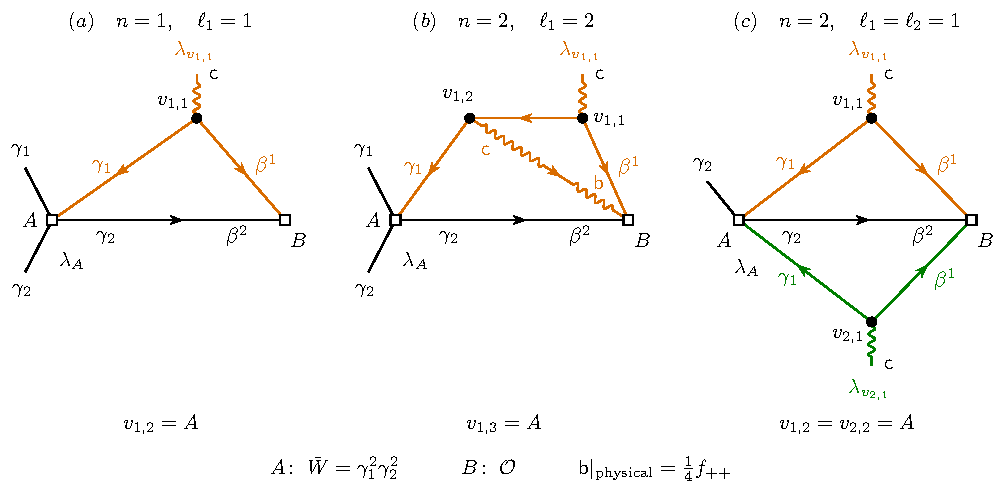
\includegraphics[width=0.96\linewidth]{figures/vec/figures-circuits-spider_general_coloured.pdf}
\caption{One- and two-loop spiders for $\bar W=\gamma_1^2\gamma_2^2$: (a) $\ell_1=1$; (b) $\ell_1=2$; (c) $\ell_1=\ell_2=1$. The superpotential vertex is $A$ and the operator insertion is $B$; each arm, with its spokes, has its own colour. Arm indices increase towards $A=v_{i,\ell_i+1}$. Each $v_{i,1}$ carries an output $\mathsf c$; the output matter at $A$ supplies $\lambda_A$.}
\label{fig-spider}
\end{figure}

On arm $i$, $v_{i,1}$ carries the source, $v_{i,\ell_i}$ is adjacent to $A$, and $v_{i,\ell_i+1}=A$. The remaining arm vertices are fully contracted:
\begin{equation}\label{eq-1-47}
\begin{gathered}
I=\big((v_{i,j},v_{i,j+1}),(v_{i,j},B)\big)_{i=1,\ldots,a;\ j=1,\ldots,\ell_i}
\cup\{(A,B)\},\\
\ell_1+\cdots+\ell_a=n,\qquad
\lambda_{v_{i,j},+\dot a}=\delta_{j1}\lambda_{v_{i,1},+\dot a}.
\end{gathered}
\end{equation}

All computations of $Q_n$ involve only the spider kernel. The computation of the spider kernel is similar to repeating the computation of the fan kernel on each path.

\rthm{Theorem}{thm-spider-kernel}{Spider kernel at every loop order} \emph{For the spider \eqref{eq-1-47} with arms of lengths $\ell_1,\ldots,\ell_a$, $\ell_1+\cdots+\ell_a=n$, sources $\lambda_A$ and $\lambda_{v_{i,1}}$, and arbitrary displacements $z_e$, in the coordinates}
\begin{equation}\label{eq-spiderdomain}
0<r_{i,j}<1\quad(j<2\ell_i),\qquad
r_{i,2\ell_i}>0,\qquad\sum_i r_{i,2\ell_i}<1.
\end{equation}
\emph{the kernel is}
\begin{equation}\label{eq-1-54}
\begin{aligned}
\mathcal I_\Gamma(\lambda;z)
={}&\int_{\eqref{eq-spiderdomain}}\prod_{i=1}^a\prod_{j=1}^{2\ell_i}dr_{i,j}\,
\underbrace{\left(1-\sum_i r_{i,2\ell_i}\right)}_{\text{final parallel merge}}\\
&\times\prod_{i=1}^a\,
\underbrace{r_{i,2\ell_i}^{\ell_i-1}\prod_{j=1}^{\ell_i-1}\Big[r_{i,2j-1}^{\ell_i-j}\,r_{i,2j}^{\,j-1}\,(1-r_{i,2j})\Big]
\bigl[\lambda_{v_{i,1},+\dot a}y^{\mathrm{red}}_{AB,+}{}^{\dot a}\bigr]^{\ell_i}}_{\text{diagonal blocks of arm }i}
\,e^{-\sum_e y_{e,+\dot a}(r)z_e^{+\dot a}},
\end{aligned}
\end{equation}
\emph{where the final resistor carries the reduced current}
\begin{equation}\label{eq-spider-reduced}
y^{\mathrm{red}}_{AB,+\dot a}
=\lambda_{A,+\dot a}+\sum_i
\left(\prod_{k=1}^{\ell_i}r_{i,2k-1}\right)\lambda_{v_{i,1},+\dot a}.
\end{equation}
\emph{Reversing the reduction on each arm, from $A$ outwards, gives the reduced spoke currents and then all currents, polynomial in $r$: with $v_{i,\ell_i+1}=A$ and $y^{\mathrm{red}}_{v_{i,\ell_i+1}B}=y^{\mathrm{red}}_{AB}$,}
\begin{equation}\label{eq-spider-reconstruction-recurrence}
y^{\mathrm{red}}_{v_{i,j}B,+\dot a}
=(1-r_{i,2j-1})\left(\prod_{k=1}^{j-1}r_{i,2k-1}\right)\lambda_{v_{i,1},+\dot a}
+r_{i,2j}\,y^{\mathrm{red}}_{v_{i,j+1}B,+\dot a}\qquad(1\le j\le\ell_i),
\end{equation}
\begin{equation}\label{eq-1-51}
\begin{aligned}
y_{v_{i,j}v_{i,j+1},+\dot a}
&=\left(\prod_{k=1}^{j-1}r_{i,2k-1}\right)\lambda_{v_{i,1},+\dot a}
-y^{\mathrm{red}}_{v_{i,j}B,+\dot a},\\
y_{v_{i,1}B,+\dot a}&=y^{\mathrm{red}}_{v_{i,1}B,+\dot a},\\
y_{v_{i,j}B,+\dot a}
&=(1-r_{i,2j-2})y^{\mathrm{red}}_{v_{i,j}B,+\dot a}\quad(j\ge2),\\
y_{AB,+\dot a}
&=\left(1-\sum_i r_{i,2\ell_i}\right)y^{\mathrm{red}}_{AB,+\dot a}.
\end{aligned}
\end{equation}
\emph{Every coefficient of the displacement expansion is the explicit finite factorial sum \eqref{eq-spider-full-taylor}.}

Here $r_{i,2j-1}$ is the fraction of the source at $v_{i,j}$, after the earlier eliminations, that the series step passes to $v_{i,j+1}$, the rest going to $B$; for $j<\ell_i$, $r_{i,2j}$ is the fraction of the merged spoke current at $v_{i,j+1}$ carried by the new branch; and $r_{i,2\ell_i}$ is the fraction of the final current carried by the branch of arm $i$, the original edge $AB$ carrying $1-\sum_ir_{i,2\ell_i}$. The final resistor carries the reduced current $y^{\mathrm{red}}_{AB}$, which by conservation at $A$ is the source collected at $A$: $\lambda_A$ and, from each arm, the fraction of its source passed along the whole arm, \eqref{eq-spider-reduced}.

Each arm is reduced as a fan is, from its outer end (Figure~\ref{fig-spider-reduction}).

\begin{figure}[H]
\centering
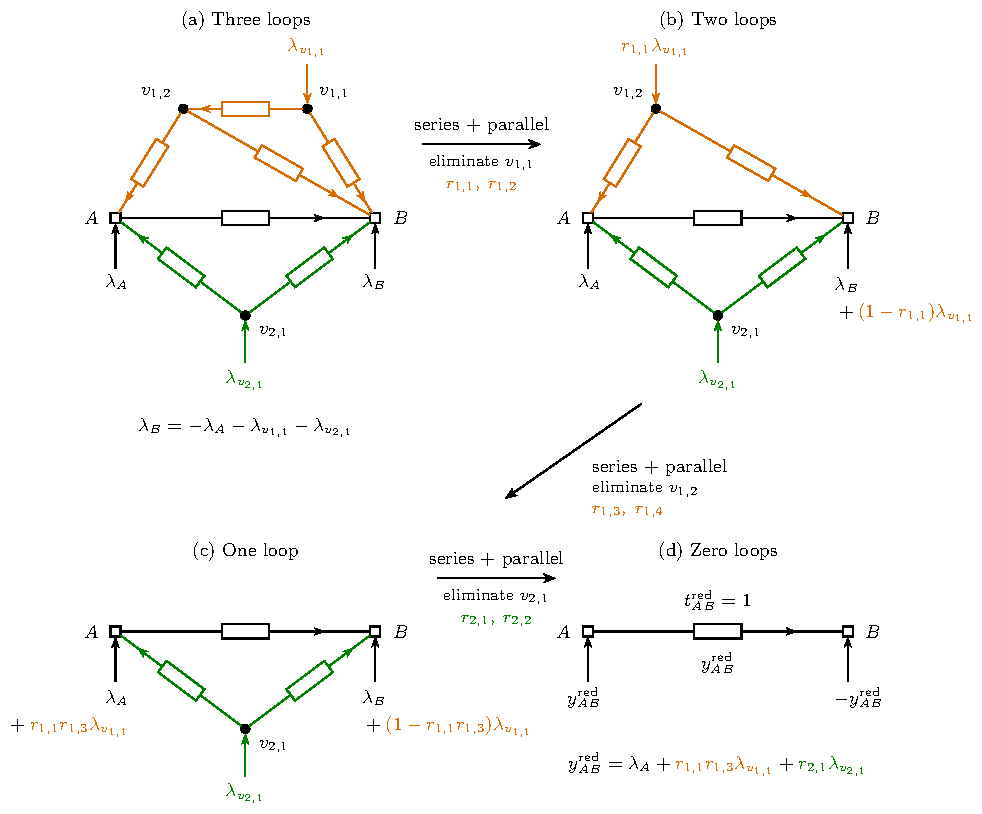
\includegraphics[width=0.96\linewidth]{figures/vec/figures-circuits-spider_reduction.pdf}
\caption{Reduction of the three-loop spider with arms $\ell_1=2$ (orange) and $\ell_2=1$ (green). Each step eliminates an arm vertex by a series step, which passes the fraction $r_{i,2j-1}$ of its source along the arm and the rest to $B$, and a parallel merge with the next spoke or with $AB$; each step lowers the loop number by one. The last panel is the unit resistor carrying \eqref{eq-spider-reduced}.}
\label{fig-spider-reduction}
\label{fig-sum-spider}
\end{figure}

Each merge lowers the loop number by one. When every arm is reduced, its branch and the original edge $AB$ merge into one resistor, whose Schwinger time is fixed to one.

\subsubsection{Iterating the series--parallel operators}\label{sec-spider-reduction}

For the spider \eqref{eq-1-47}, apply \eqref{eq-kernel-series-parallel} along each arm, then remove the book pages until one triangle remains.

Eliminate the interior vertices $v_{i,1},\ldots,v_{i,\ell_i-1}$, arm by arm, followed by the terminal vertices $v_{1,\ell_1},\ldots,v_{a-1,\ell_{a-1}}$; put $v_{i,\ell_i+1}=A$ and $u=v_{i,j+1}$ when $v=v_{i,j}$.

Each factor below has its own local parameters $r_1,r_2$ of \eqref{eq-kernel-series-parallel}, acts on everything to its right, and substitutes the source and displacement updates after differentiating:
\begin{equation*}
\begin{aligned}
    \mathcal I_\Gamma(\lambda;z)
    ={}&\prod_{\substack{v\ \mathrm{in\ the\ displayed\ elimination\ order}}}
    \Biggl[
    \int_0^1dr_1\int_0^1dr_2\,
    e^{-\lambda_{v,+\dot a}^{\mathrm{red}}
    [r_1z_{vu}+(1-r_1)z_{vB}^{\mathrm{red}}]^{+\dot a}}\\
    &\hspace{42mm}\times r_2\lambda_{v,+}^{\mathrm{red}}{}^{\dot b}
    \frac{\partial}{\partial z_{uB}^{\mathrm{red},+\dot b}}
    \Biggr]
    \underbrace{\mathcal I_\triangle
    (\lambda^{\mathrm{red}};z^{\mathrm{red}})}_{\substack{\text{vertices }v_{a,\ell_a},A,B\\\text{known one-loop kernel \eqref{eq-1-25}}}}.
    \end{aligned}
\end{equation*}

Here $v=v_{i,j}$, $u=v_{i,j+1}$ and $w=B$ in Theorem~\ref{b-01142}, with the updates
\begin{equation*}
\begin{gathered}
\lambda_u^{\mathrm{red}}=\lambda_u+r_1\lambda_v,\qquad
\lambda_B^{\mathrm{red}}=\lambda_B+(1-r_1)\lambda_v,\\
z_{uB}^{\mathrm{red}}=r_2z_{uB}+(1-r_2)(z_{vB}-z_{vu}),
\qquad z_e^{\mathrm{red}}=z_e\quad(e\ne uB).
\end{gathered}
\end{equation*}

We evaluate these derivatives before expanding the final exponential.

\subsubsection{Derivatives along an arm}\label{local-B5-arms-heading}

The internal arm sources vanish as in \eqref{eq-1-47}, and $v_{i,\ell_i+1}=A$.
\begin{equation}\label{eq-spider-reduced-data}
\begin{aligned}
\lambda_{v_{i,j+1},+\dot a}^{\mathrm{red}}
&=r_{i,2j-1}\lambda_{v_{i,j},+\dot a}^{\mathrm{red}}
\qquad(j<\ell_i),\\
\lambda_{v_{i,j},+\dot a}^{\mathrm{red}}
&=\left(\prod_{k=1}^{j-1}r_{i,2k-1}\right)
\lambda_{v_{i,1},+\dot a},\qquad 1\le j\le\ell_i.
\end{aligned}
\end{equation}

For $j<\ell_i$, use \eqref{eq-kernel-series-parallel} with $(v,u,w)=(v_{i,j},v_{i,j+1},B)$ and local parameters $(r_1,r_2)=(r_{i,2j-1},1-r_{i,2j})$.

Each superscript $\mathrm{red}$ refers to the circuit at the indicated step; the incoming source and spoke displacement already include the preceding reductions.
\begin{equation*}
\begin{aligned}
\mathcal I_\Gamma(\lambda;z)
={}&\int_0^1dr_{i,2j-1}\int_0^1dr_{i,2j}\\
&\times e^{-\lambda^{\mathrm{red}}_{v_{i,j},+\dot a}
[r_{i,2j-1}z_{v_{i,j}v_{i,j+1}}+(1-r_{i,2j-1})z_{v_{i,j}B}^{\mathrm{red}}]^{+\dot a}}\\
&\times\underbrace{(1-r_{i,2j})\lambda^{\mathrm{red}}_{v_{i,j},+}{}^{\dot b}
\frac{\partial}{\partial z_{v_{i,j+1}B}^{\mathrm{red},+\dot b}}}_{\text{operator supplied by \eqref{eq-kernel-series-parallel}}}
\underbrace{\mathcal I_{\Gamma^{\mathrm{red}}}
(\lambda^{\mathrm{red}};z^{\mathrm{red}})}_{\text{one fewer arm vertex and loop}}.
\end{aligned}
\end{equation*}
\begin{equation*}
z_{v_{i,j+1}B}^{\mathrm{red}}
=(1-r_{i,2j})z_{v_{i,j+1}B}
+r_{i,2j}\bigl(z_{v_{i,j}B}^{\mathrm{red}}-z_{v_{i,j}v_{i,j+1}}\bigr).
\end{equation*}

The later source on the same arm is a multiple of $\lambda_{v_{i,1}}$, so an earlier directional derivative annihilates its source phase:
\begin{equation*}
\lambda_{v_{i,1},+\dot a}\lambda_{v_{i,k},+}^{\mathrm{red}}{}^{\dot a}=0.
\end{equation*}
\begin{equation*}
\lambda_{v_{i,1},+}{}^{\dot a}
    \frac{\partial}{\partial z_{v_{i,k}B}^{\mathrm{red},+\dot a}}
     e^{-\lambda_{v_{i,k},+\dot b}^{\mathrm{red}}
    [r_{i,2k-1}z_{v_{i,k}v_{i,k+1}}+(1-r_{i,2k-1})z_{v_{i,k}B}^{\mathrm{red}}]^{+\dot b}}=0.
\end{equation*}

Its action on the next kernel passes through the affine displacement substitution:
\begin{equation*}
\lambda_{v_{i,1},+}{}^{\dot a}
\frac{\partial}{\partial z_{v_{i,k}B}^{\mathrm{red},+\dot a}}
=r_{i,2k}\lambda_{v_{i,1},+}{}^{\dot a}
\frac{\partial}{\partial z_{v_{i,k+1}B}^{\mathrm{red},+\dot a}}
\qquad(k<\ell_i).
\end{equation*}

Repeat for $j=1,\ldots,\ell_i-1$ on each arm; the remaining graph is the book on $A,B,v_{1,\ell_1},\ldots,v_{a,\ell_a}$.

\subsubsection{Evaluate the book from one triangle}\label{sec-book-jacobian}

Use the book labels $1,\ldots,n$, $A=n+1$, $B=n+2$, with $n=a$ pages and $\lambda_i=\lambda_{v_{i,\ell_i}}^{\mathrm{red}}$.

Remove pages $1,\ldots,n-1$, leaving the triangle $(n,A,B)$; the sources and the $AB$ displacement update at each step by
\begin{equation*}
\begin{aligned}
\left.\lambda_A^{\mathrm{red}}\right|_{\text{after }i}
&=\left.\lambda_A^{\mathrm{red}}\right|_{\text{before }i}+r_1\lambda_i,\\
\left.\lambda_B^{\mathrm{red}}\right|_{\text{after }i}
&=\left.\lambda_B^{\mathrm{red}}\right|_{\text{before }i}+(1-r_1)\lambda_i,\\
\left.z_{AB}^{\mathrm{red}}\right|_{\text{after }i}
&=r_2\left.z_{AB}^{\mathrm{red}}\right|_{\text{before }i}
+(1-r_2)(z_{iB}-z_{iA}).
\end{aligned}
\end{equation*}

The later page phases are independent of $z_{AB}^{\mathrm{red}}$; therefore the composed derivatives act directly on the known triangle kernel:
\begin{equation}\label{eq-B-book-full-kernel}
\begin{aligned}
    \mathcal I_\Gamma(\lambda;z)
    ={}&\int_{(0,1)^{2n-2}}
    \prod_{i=1}^{n-1}\left[d\!\left(\left.r_1\right|_{v=i}\right)
     d\!\left(\left.r_2\right|_{v=i}\right)\right]\\
    &\times e^{-\sum_{\substack{1\le i<n\\\mathrm{removed\ pages}}}
    \lambda_{i,+\dot a}
    [(\left.r_1\right|_{v=i})z_{iA}+(1-\left.r_1\right|_{v=i})z_{iB}]^{+\dot a}}\\
    &\times\prod_{i=1}^{n-1}\left[
    \left(\prod_{k=i}^{n-1}\left.r_2\right|_{v=k}\right)
    \lambda_{i,+}{}^{\dot a_i}
    \frac{\partial}{\partial z_{AB}^{\mathrm{red},+\dot a_i}}
    \right]
    \underbrace{\mathcal I_\triangle(\lambda^{\mathrm{red}};z^{\mathrm{red}})}_{(n,A,B)}.
    \end{aligned}
\end{equation}

The product of local $r_2$ factors follows at every substitution from
\begin{equation*}
\left.\frac{\partial}{\partial z_{AB}^{\mathrm{red},+\dot a}}\right|_{\mathrm{before\ page}\ k}
    =\left.r_2\right|_{v=k}
    \left.\frac{\partial}{\partial z_{AB}^{\mathrm{red},+\dot a}}\right|_{\mathrm{after\ page}\ k}.
\end{equation*}

In the last triangle, use the local coordinates $r_1,r_2$ of \eqref{eq-1-25}; its currents are
\begin{equation*}
\begin{aligned}
    y_{nA,+\dot a}^{\mathrm{red}}&=r_1\lambda_{n,+\dot a}-r_2\lambda_{A,+\dot a}^{\mathrm{red}},\\
    y_{nB,+\dot a}^{\mathrm{red}}&=\lambda_{n,+\dot a}-y_{nA,+\dot a}^{\mathrm{red}},\\
    y_{AB,+\dot a}^{\mathrm{red}}&=(1-r_2)\lambda_{A,+\dot a}^{\mathrm{red}}+r_1\lambda_{n,+\dot a}.
    \end{aligned}
\end{equation*}

Every derivative in \eqref{eq-B-book-full-kernel} inserts this $AB$ current:
\begin{equation*}
\begin{aligned}
    &\prod_{i=1}^{n-1}
    \left[\lambda_{i,+}{}^{\dot a_i}
    \frac{\partial}{\partial z_{AB}^{\mathrm{red},+\dot a_i}}\right]
    \mathcal I_\triangle(\lambda^{\mathrm{red}};z^{\mathrm{red}})\\
    &=\bigl(\lambda_{n,+\dot b}\lambda_{A,+}^{\mathrm{red}}{}^{\dot b}\bigr)
    \int_0^1dr_1\int_0^{1-r_1}dr_2\,
    \prod_{i=1}^{n-1}
    \bigl(\lambda_{i,+\dot a_i}y_{AB,+}^{\mathrm{red}}{}^{\dot a_i}\bigr)
     e^{-\sum_{\substack{e\in\{nA,nB,AB\}\\\mathrm{triangle\ edges}}}
     y_{e,+\dot c}^{\mathrm{red}}z_e^{\mathrm{red},+\dot c}}.
    \end{aligned}
\end{equation*}

To write the result in the current shares of \eqref{eq-spiderdomain}, include the final triangle's local parameters and use
\begin{equation*}
\left.r_1\right|_{v=n}=\frac{r_1}{1-r_2},\qquad
    \left.r_2\right|_{v=n}=1-r_2.
\end{equation*}
\begin{equation*}
\begin{aligned}
    \left.y_{AB,+\dot a}^{\mathrm{red}}\right|_{\mathrm{triangle}}
    &=\left.r_2\right|_{v=n}
    \left.y_{AB,+\dot a}^{\mathrm{red}}\right|_{\mathrm{final\ edge}},\\
    \lambda_{n,+\dot a}
    \left.\lambda_{A,+}^{\mathrm{red}}{}^{\dot a}\right|_{\mathrm{triangle}}
    &=\lambda_{n,+\dot a}
    \left.y_{AB,+}^{\mathrm{red}}{}^{\dot a}\right|_{\mathrm{final\ edge}}.
    \end{aligned}
\end{equation*}
\begin{equation}\label{eq-book-current-derivative}
\begin{gathered}
\left.r_1\right|_{v=i}=r_{2i-1},\qquad
\left.r_2\right|_{v=i}
=\frac{1-\sum_{\substack{i\le k\le n\\\mathrm{pages}}}r_{2k}}
{1-\sum_{\substack{i<k\le n\\\mathrm{pages}}}r_{2k}},\\[3pt]
r_{2i}=\left(1-\left.r_2\right|_{v=i}\right)
\prod_{k=i+1}^{n}\left.r_2\right|_{v=k}.
\end{gathered}
\end{equation}

The resulting currents are
\begin{equation}\label{eq-B-book-reduced-current}
\begin{aligned}
y^{\mathrm{red}}_{n+1,n+2,+\dot a}
&=\lambda_{n+1,+\dot a}+\sum_{j=1}^n r_{2j-1}\lambda_{j,+\dot a},\\
y_{i,n+1,+\dot a}
&=r_{2i-1}\lambda_{i,+\dot a}
-r_{2i}y^{\mathrm{red}}_{n+1,n+2,+\dot a},\\
y_{i,n+2,+\dot a}
&=(1-r_{2i-1})\lambda_{i,+\dot a}
+r_{2i}y^{\mathrm{red}}_{n+1,n+2,+\dot a},\\
y_{n+1,n+2,+\dot a}
&=\left(1-\sum_i r_{2i}\right)y^{\mathrm{red}}_{n+1,n+2,+\dot a}.
\end{aligned}
\end{equation}

The successive derivatives and the last triangle supply $\prod_{i=1}^n(\left.r_2\right|_{v=i})^i$; substituting \eqref{eq-book-current-derivative} gives the positive integration densities
\begin{equation*}
\begin{aligned}
    &\prod_{i=1}^{n}\left[
    \left(\left.r_2\right|_{v=i}\right)^i
    \left|d\!\left(\left.r_2\right|_{v=i}\right)\right|\right]\\
    &=\frac{\displaystyle\prod_{i=1}^{n}
    \left(1-\sum_{\substack{i\le k\le n\\\mathrm{pages}}}r_{2k}\right)}
    {\displaystyle\prod_{i=1}^{n}
    \left(1-\sum_{\substack{i<k\le n\\\mathrm{pages}}}r_{2k}\right)}
    \prod_{i=1}^{n}dr_{2i}\\
    &=\left(1-\sum_{\substack{1\le i\le n\\\mathrm{pages}}}r_{2i}\right)
    \prod_{i=1}^{n}dr_{2i}.
    \end{aligned}
\end{equation*}

The phase substitutions restore the original edge exponential, and the accumulated operators give
\begin{equation}\label{eq-book-current-determinant}
\begin{aligned}
    \mathcal I_\Gamma(\lambda;z)
    ={}&\int_{\substack{0<r_{2i-1}<1\\r_{2i}>0,\ \sum_{\substack{1\le i\le n\\\mathrm{pages}}}r_{2i}<1}}
    \prod_{i=1}^n(dr_{2i-1}\,dr_{2i})\,
    \left(1-\sum_{\substack{1\le i\le n\\\mathrm{pages}}}r_{2i}\right)\\
    &\times\prod_{i=1}^{n}
    \bigl(\lambda_{i,+\dot a_i}y_{AB,+}^{\mathrm{red}}{}^{\dot a_i}\bigr)
     e^{-\sum_{\substack{e\in I\\\mathrm{edges}}}y_{e,+\dot b}z_e^{+\dot b}}.
    \end{aligned}
\end{equation}

For the marked product, set $z_{AB}=0$ after differentiating.

\subsubsection{Multiply the arm factors}\label{local-B5-complete-heading}

Restore the spider labels, $n=\sum_{\substack{1\le i\le a\\\mathrm{arms}}}\ell_i$; at the book, the final $AB$ displacement contains the terminal spoke with coefficient $r_{i,2\ell_i}$.

Combining this coefficient with the successive arm derivatives gives the contribution from vertex $v_{i,j}$:
\begin{equation}\label{eq-spider-jacobian-blocks}
\begin{gathered}
(1-r_{i,2j})
\left(\prod_{k=1}^{j-1}r_{i,2k-1}\right)
\left(\prod_{k=j+1}^{\ell_i-1}r_{i,2k}\right)
r_{i,2\ell_i}
\bigl(\lambda_{v_{i,1},+\dot a}y_{AB,+}^{\mathrm{red}}{}^{\dot a}\bigr),
\qquad j<\ell_i.
\end{gathered}
\end{equation}

The terminal page contributes $\bigl(\prod_{k=1}^{\ell_i-1}r_{i,2k-1}\bigr)\bigl(\lambda_{v_{i,1},+\dot a}y_{AB,+}^{\mathrm{red}}{}^{\dot a}\bigr)$; the remaining coefficients multiply as
\begin{equation}\label{eq-spider-final-block}
\begin{aligned}
&\left[\prod_{j=1}^{\ell_i-1}
(1-r_{i,2j})
\left(\prod_{k=1}^{j-1}r_{i,2k-1}\right)
\left(\prod_{k=j+1}^{\ell_i-1}r_{i,2k}\right)
r_{i,2\ell_i}\right]
\left(\prod_{k=1}^{\ell_i-1}r_{i,2k-1}\right)\\
&\qquad=r_{i,2\ell_i}^{\ell_i-1}
\prod_{j=1}^{\ell_i-1}
\left[r_{i,2j-1}^{\ell_i-j}r_{i,2j}^{j-1}(1-r_{i,2j})\right].
\end{aligned}
\end{equation}

The source phases and reduced exponents combine as in \eqref{eq-book-current-determinant}; the evaluated integral is \eqref{eq-1-54}, and every factor comes from a displayed derivative acting on the remaining kernel.

\subsubsection{Recover the currents by the same iteration}\label{sec-spider-jacobian}

The final transferred source determines the final edge current \eqref{eq-spider-reduced}. Reversing the current update in \eqref{eq-kernel-series-parallel}, starting at each terminal page, gives the recurrence \eqref{eq-spider-reconstruction-recurrence}, with the reduced sources \eqref{eq-spider-reduced-data}. Its solution is
\begin{equation}\label{eq-1-50}
\begin{aligned}
y^{\mathrm{red}}_{v_{i,j}B,+\dot a}
={}&\sum_{r=j}^{\ell_i}
\left(\prod_{k=j}^{r-1}r_{i,2k}\right)(1-r_{i,2r-1})
\left(\prod_{k=1}^{r-1}r_{i,2k-1}\right)\lambda_{v_{i,1},+\dot a}\\
&+\left(\prod_{k=j}^{\ell_i-1}r_{i,2k}\right)r_{i,2\ell_i}\,
y^{\mathrm{red}}_{AB,+\dot a}.
\end{aligned}
\end{equation}
and the original currents \eqref{eq-1-51} along the arms and the exponent are
\begin{equation}\label{eq-spider-arm-current}
\begin{aligned}
y_{v_{i,j}v_{i,j+1},+\dot a}
={}&\sum_{s=j}^{\ell_i-1}
\left(\prod_{k=1}^{s}r_{i,2k-1}\right)
\left(\prod_{k=j}^{s-1}r_{i,2k}\right)(1-r_{i,2s})\,
\lambda_{v_{i,1},+\dot a}\\
&+\left(\prod_{k=1}^{\ell_i}r_{i,2k-1}\right)
\left(\prod_{k=j}^{\ell_i-1}r_{i,2k}\right)
\lambda_{v_{i,1},+\dot a}
-\left(\prod_{k=j}^{\ell_i}r_{i,2k}\right)
y^{\mathrm{red}}_{AB,+\dot a}.
\end{aligned}
\end{equation}
\begin{equation}\label{eq-spider-loop-split}
\begin{aligned}
\sum_e y_{e,+\dot a}z_e^{+\dot a}
={}&\lambda_{A,+\dot a}z_{AB}^{+\dot a}
+\sum_i\lambda_{v_{i,1},+\dot a}z_{v_{i,1}B}^{+\dot a}\\
&+\sum_{i=1}^a\sum_{j=1}^{\ell_i}
y_{v_{i,j}v_{i,j+1},+\dot a}
(z_{v_{i,j}v_{i,j+1}}+z_{v_{i,j+1}B}-z_{v_{i,j}B})^{+\dot a},
\qquad v_{i,\ell_i+1}=A.
\end{aligned}
\end{equation}

\subsubsection{Output translation and Taylor expansion}

The cubic arm vertices carry no derivatives, so $z_{v_{i,j}v_{i,j+1}}=0$ for $j<\ell_i$; the spokes, the last arm edges and $AB$ keep general displacements if we want to compute results with holomorphic derivatives.

The exponential then translates the outputs at $v_{i,1}$ and $A$:
\begin{equation}\label{eq-spider-output-translation}
-\sum_e y_{e,+\dot a}(r)z_e^{+\dot a}
=\lambda_{A,+\dot a}x_A^{+\dot a}(r,z)
+\sum_{i=1}^a\lambda_{v_{i,1},+\dot a}x_{v_{i,1}}^{+\dot a}(r,z),
\end{equation}
with translated positions
\begin{equation}\label{eq-spider-output-points}
\begin{aligned}
x_A^{+\dot a}(r,z)
={}&-\left(1-\sum_i r_{i,2\ell_i}\right)z_{AB}^{+\dot a}\\
&-\sum_{i=1}^a r_{i,2\ell_i}\left[
\sum_{j=1}^{\ell_i}(1-r_{i,2j-2})
\left(\prod_{k=j}^{\ell_i-1}r_{i,2k}\right)z_{v_{i,j}B}^{+\dot a}
-z_{v_{i,\ell_i}A}^{+\dot a}\right],\\[3pt]
x_{v_{i,1}}^{+\dot a}(r,z)
={}&-\sum_{s=1}^{\ell_i}(1-r_{i,2s-1})
\left(\prod_{k=1}^{s-1}r_{i,2k-1}\right)
\sum_{j=1}^{s}(1-r_{i,2j-2})
\left(\prod_{k=j}^{s-1}r_{i,2k}\right)z_{v_{i,j}B}^{+\dot a}\\
&+\left(\prod_{k=1}^{\ell_i}r_{i,2k-1}\right)
\bigl(x_A^{+\dot a}(r,z)-z_{v_{i,\ell_i}A}^{+\dot a}\bigr),
\qquad r_{i,0}=0.
\end{aligned}
\end{equation}

For nonnegative integers $\kappa_{i,j}$ and $\bar\kappa_{i,2j}$, the weighted monomial moments on \eqref{eq-spiderdomain} are
\begin{equation}\label{eq-spider-moments}
\begin{aligned}
&\int_{\eqref{eq-spiderdomain}}\prod_{i,j}dr_{i,j}
\left(1-\sum_i r_{i,2\ell_i}\right)
\prod_{i=1}^a\Bigg[r_{i,2\ell_i}^{\ell_i-1+\kappa_{i,2\ell_i}}
\prod_{j=1}^{\ell_i}r_{i,2j-1}^{\ell_i-j+\kappa_{i,2j-1}}
\prod_{j=1}^{\ell_i-1}r_{i,2j}^{j-1+\kappa_{i,2j}}(1-r_{i,2j})^{1+\bar\kappa_{i,2j}}\Bigg]\\
&=\frac{\prod_i(\ell_i-1+\kappa_{i,2\ell_i})!}{(n+1+\sum_i \kappa_{i,2\ell_i})!}
\prod_{i=1}^a\Bigg[\prod_{j=1}^{\ell_i}\frac1{\ell_i-j+1+\kappa_{i,2j-1}}
\prod_{j=1}^{\ell_i-1}
\frac{(j-1+\kappa_{i,2j})!\,(1+\bar\kappa_{i,2j})!}{(j+1+\kappa_{i,2j}+\bar\kappa_{i,2j})!}\Bigg].
\end{aligned}
\end{equation}

We organize the final result: Sum over nonnegative integers $m_{iA}$, $m_{ik}$ $(k\ne i)$ with $m_{iA}+\sum_{k\ne i}m_{ik}=\ell_i$, $p_{ijs}$ $(1\le j\le s\le\ell_i)$, and $q_{ijA}$, $q_{ijk}$ $(1\le j\le\ell_i,\ 1\le k\le a)$, and write $q_{ij}=q_{ijA}+\sum_kq_{ijk}$ and $M_i=\sum_{k\ne i}m_{ki}+\sum_{k=1}^a\sum_{j=1}^{\ell_k}q_{kji}$.

The multinomial exponents $m_{iA}$ and $m_{ik}$ choose the $\lambda_A$ and $\lambda_{v_{k,1}}$ terms in $[\lambda_{v_{i,1}}y^{\mathrm{red}}_{AB}]^{\ell_i}$. In the displacement exponential, $p_{ijs}$ counts the $s$th $\lambda_{v_{i,1}}$ term of \eqref{eq-spider-arm-current}, including $s=\ell_i$, while $q_{ijA}$ and $q_{ijk}$ count the $\lambda_A$ and $\bigl(\prod_{h=1}^{\ell_k}r_{k,2h-1}\bigr)\lambda_{v_{k,1}}$ terms of $y^{\mathrm{red}}_{AB}$ in its last term.

With these multiplicities, the coordinate exponents in \eqref{eq-spider-moments} are
\begin{equation}\label{eq-spider-taylor-exponents}
\begin{gathered}
\kappa_{i,2t-1}=M_i+\sum_{s=t}^{\ell_i}\sum_{j=1}^{s}p_{ijs},\qquad
\kappa_{i,2t}=\sum_{j=1}^{t}\left[q_{ij}+\sum_{s=t+1}^{\ell_i}p_{ijs}\right]\ (t<\ell_i),\\
\bar\kappa_{i,2t}=\sum_{j=1}^{t}p_{ijt},\qquad
\kappa_{i,2\ell_i}=\sum_{j=1}^{\ell_i}q_{ij}.
\end{gathered}
\end{equation}

The full Taylor expansion is
\begin{equation}\label{eq-spider-full-taylor}
\begin{aligned}
&\mathcal I_\Gamma(\lambda;z)
=e^{-\lambda_{A,+\dot a}z_{AB}^{+\dot a}
-\sum_i\lambda_{v_{i,1},+\dot a}z_{v_{i,1}B}^{+\dot a}}
\sum_{m,p,q}\prod_{i=1}^a\Bigg\{\\
&\quad\hphantom{{}\times{}}\ell_i!\,
\frac{(\lambda_{v_{i,1},+\dot b}\lambda_{A,+}{}^{\dot b})^{m_{iA}}}{m_{iA}!}
\prod_{k\ne i}
\frac{(\lambda_{v_{i,1},+\dot c}\lambda_{v_{k,1},+}{}^{\dot c})^{m_{ik}}}{m_{ik}!}\\
&\quad\times\prod_{j=1}^{\ell_i}\Bigg[
\prod_{s=j}^{\ell_i}
\frac{\bigl[-\lambda_{v_{i,1},+\dot d}
(z_{v_{i,j}v_{i,j+1}}+z_{v_{i,j+1}B}-z_{v_{i,j}B})^{+\dot d}\bigr]^{p_{ijs}}}{p_{ijs}!}\\
&\qquad\times
\frac{\bigl[\lambda_{A,+\dot e}
(z_{v_{i,j}v_{i,j+1}}+z_{v_{i,j+1}B}-z_{v_{i,j}B})^{+\dot e}\bigr]^{q_{ijA}}}{q_{ijA}!}\\
&\qquad\times\prod_{k=1}^a
\frac{\bigl[\lambda_{v_{k,1},+\dot f}
(z_{v_{i,j}v_{i,j+1}}+z_{v_{i,j+1}B}-z_{v_{i,j}B})^{+\dot f}\bigr]^{q_{ijk}}}{q_{ijk}!}
\Bigg]\Bigg\}\\
&\quad\times
\frac{\prod_i\left(\ell_i-1+\sum_{j}q_{ij}\right)!}
{\left(n+1+\sum_{i,j}q_{ij}\right)!}
\prod_{i=1}^a\prod_{t=1}^{\ell_i}
\frac1{\ell_i-t+1+M_i+\sum_{s=t}^{\ell_i}\sum_{j=1}^{s}p_{ijs}}\\
&\quad\times\prod_{i=1}^a\prod_{t=1}^{\ell_i-1}
\frac{\left(t-1+\sum_{j=1}^{t}\left[q_{ij}+\sum_{s=t+1}^{\ell_i}p_{ijs}\right]\right)!\,
\left(1+\sum_{j=1}^{t}p_{ijt}\right)!}
{\left(t+1+\sum_{j=1}^{t}\left[q_{ij}+\sum_{s=t}^{\ell_i}p_{ijs}\right]\right)!}.
\end{aligned}
\end{equation}

For the physical displacements, $z_{v_{i,j}v_{i,j+1}}=0$ for $j<\ell_i$. Taking one arm gives the Taylor coefficients of \eqref{eq-fan-full-taylor}, which is exactly the fan kernel result. (A fan is a special type of spider.)

\subsection{Restrictions on quantum-product graphs}\label{sec-dressed-definition}

The graphs of the quantum product \eqref{b-00504} are forests of interaction trees attached to both insertions. We first bound their superpotential vertices, with the counting of Section \ref{sec-spider-classification}, and then classify them.

\rthm{Proposition}{b-00249}{Superpotential vertices in quantum product diagrams} \emph{Let $\Gamma$ be a nonzero connected marked graph of the quantum product \eqref{b-00504} at order $\hbar^n$, $n\ge1$, with insertions $A,B$, two arbitrary composite operators.}

(i) \emph{Every connected component of $\Gamma\setminus\{A,B\}$ contains at most one $\bar W$ vertex.}

(ii) \emph{Each graph term satisfies}
\begin{equation}\label{eq-product-antifield-loss}
\#(\mathsf b,\beta\text{ in the output})
=\#(\mathsf b,\beta\text{ in }A)+\#(\mathsf b,\beta\text{ in }B)-n-\#(\bar W\text{ vertices}),
\end{equation}
\emph{so the order-$\hbar^n$ term vanishes unless $\#(\mathsf b,\beta\text{ in }A)+\#(\mathsf b,\beta\text{ in }B)\ge n+\#(\bar W\text{ vertices})$.}

\emph{Proof.} (i) The $|T_j|$ nodes of a component $T_j$ are connected through its internal resistors $I_j$, each of which takes its antifield terminal from a node of $T_j$ (Lemma~\ref{local-3f6d7139-9e21-4d1f-95cc-7d06f9c41ebc}):
\begin{equation*}
|T_j|-1\le|I_j|\le|T_j|-\#(\bar W\text{ vertices in }T_j).
\end{equation*}

(ii) Each of the $2n$ physical resistors takes one antifield terminal; the $n$ interaction nodes have $n-\#(\bar W\text{ vertices})$ of them.~\hfill\qedsymbol

\rthm{Proposition}{b-00344}{Edge counts of the product graphs} \emph{Let $\Gamma$ be a nonzero connected marked graph of \eqref{b-00504} at order $\hbar^n$, $n\ge1$. } \emph{It has $n$ interaction vertices, the two insertions $A,B$, and $2n+1$ edges: the auxiliary edge $AB$, which contributes its kernel, and $2n$ edges contracting fields in $\mathcal I$, $A$ and $B$. } \emph{Removing $A$ and $B$ leaves the interaction subgraph (Figure~\ref{fig-forests}). } \emph{For one of its components $T_j$, with $|T_j|$ vertices, $I_j$ denotes its internal edges and $E_j$ its edges to $A$ or $B$, the spokes. } \emph{Every edge other than $AB$ is an internal edge or a spoke of exactly one component, and}
\begin{equation}\label{eq-1-20}
|T_j|-1\;\le\;|I_j|\;\le\;|T_j|-\#(\bar W\text{ vertices in }T_j),\qquad
|I_j|+|E_j|=2|T_j|.
\end{equation}

\emph{Proof.} In the circuit of $\Gamma$ (Remark~\ref{b-00176}) every edge is a resistor, and the marked resistor joins the insertions $A$ and $B$.

\emph{Internal resistors.}
\begin{equation*}
\underbrace{|T_j|-1}_{T_j\text{ connected}}
\;\le\;|I_j|\;\le\;
\underbrace{|T_j|-\#(\bar W\text{ vertices in }T_j)}_{\text{antifield terminals in }T_j}.
\end{equation*}

It is the antifield-terminal count of Lemma \ref{local-3f6d7139-9e21-4d1f-95cc-7d06f9c41ebc}.

\emph{Resistors at the insertions.} A physical resistor between $A$ and $B$ would be in parallel with the marked resistor (Corollary~\ref{b-00188}). Every physical resistor therefore ends at an interaction node, and it is an internal resistor or a spoke of the component of that node. Summing over the components,
\begin{equation}\label{eq-product-edge-sum}
\sum_j\bigl(|I_j|+|E_j|\bigr)=2n=2\sum_j|T_j|.
\end{equation}

\emph{Local Ohm's law on $T_j\cup\{A,B\}$.} The subcircuit formed by the nodes of $T_j$, the two insertions and the marked resistor obeys the local count of Ohm's law (Lemma~\ref{b-00194}):
\begin{equation*}
\begin{aligned}
&|I_j|+|E_j|+\underbrace{1}_{AB}\;\le\;2(|T_j|+2)-3\\
\Longrightarrow\quad&|I_j|+|E_j|\;\le\;2|T_j|.
\end{aligned}
\end{equation*}

By \eqref{eq-product-edge-sum}, equality holds for every component.~\hfill\qedsymbol

\begin{figure}[H]
\centering
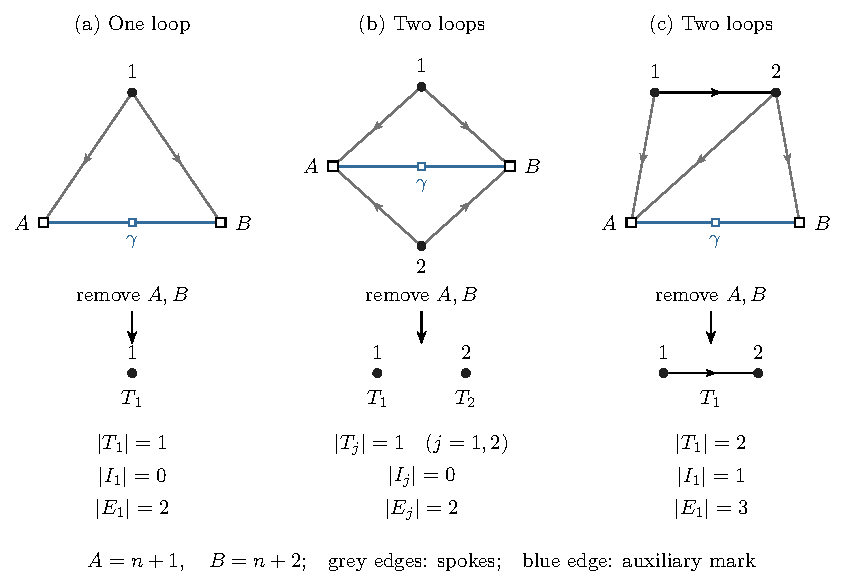
\includegraphics[width=0.89\linewidth]{figures/vec/figures-circuits-product_forest.pdf}
\caption{Marked graph topologies through two loops and their internal forests. The squares $A=n+1$ and $B=n+2$ are the two operator insertions; the blue edge carries the auxiliary mark $\gamma$. Deleting $A,B$ and all incident edges leaves (a) one isolated vertex, (b) two isolated vertices, and (c) a two-vertex tree. The black edge is internal; the grey edges are spokes to the insertions. The displayed spoke counts refer to the full graphs in the top row.}
\label{fig-forests}
\end{figure}

\begin{figure}[H]
\centering
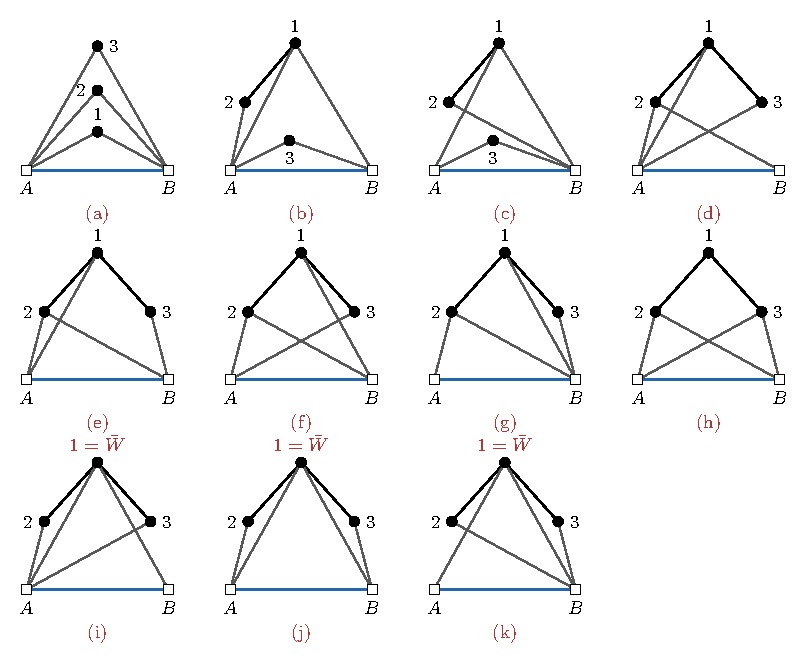
\includegraphics[width=0.85\linewidth]{figures/vec/ch6-three-loop-atlas-20261102.pdf}
\caption{All eleven marked three-loop topologies up to permutations of the interaction vertices, fixing $A$ and $B$. Panels (a)--(h) allow cubic interactions; in (i)--(k), vertex $1$ is a superpotential vertex with four resistors. Blue: the marked edge $AB$; black: internal edges; gray: spokes.}
\label{fig-product-three-loop-atlas}
\end{figure}

\rthm{Proposition}{b-00355}{Graphs of the quantum product} \emph{For the interaction \eqref{eq-B-10}, with $\bar W$ of any degree, let $\Gamma$ be a nonzero connected marked graph of \eqref{b-00504} at order $\hbar^n$, $n\ge1$. } \emph{Then}
\begin{equation}\label{eq-1-19}
\Gamma\setminus\{A,B\}=\coprod_jT_j,\qquad T_j\text{ a tree},\qquad
\#(\bar W\text{ vertices in }T_j)\leq1,\qquad
|E_j|=|T_j|+1.
\end{equation}

\emph{Every $T_j$ is joined to both $A$ and $B$, and loop diagrams contain no quadratic term of the superpotential $\bar W$ (only terms of at least cubic degree enter the theory). Each tree has one uncontracted field if all its vertices are cubic, and $\deg\bar W-2$ if it contains a superpotential monomial; its number of source-bearing vertices is bounded by that number.} See Figure~\ref{fig-sum-forests}.

\begin{figure}[H]
\centering
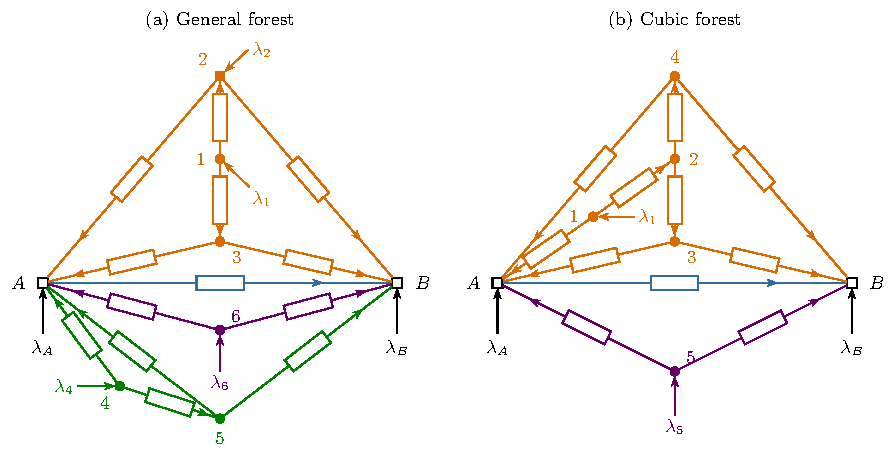
\includegraphics[width=0.95\linewidth]{figures/vec/figures-circuits-sum_forests.pdf}
\caption{Graphs of the quantum product: the marked edge $AB$ (blue) between the insertions and a forest of interaction trees, each in its own colour and joined to $A$ and $B$ by one more spoke than it has vertices. (a) For general $\bar W$, each tree contains at most one $\bar W$ vertex (square). (b) For cubic interactions, each tree carries one source, at its vertex of degree two.}
\label{fig-sum-forests}
\end{figure}

\emph{Proof.}

The proof parallels that of Proposition \ref{b-00210}.

\emph{Components without sources.} Suppose that no current is injected at the nodes of $T_j$ (Figure~\ref{fig-sourceless}(a)). The component touches the rest of the circuit only at the insertions $A$ and $B$, so the current $J$ that enters it at $A$ leaves it at $B$, and inside it Kirchhoff's laws are those of a passive network driven by $J$. Every current of the component is therefore a real multiple $c_eJ$ of $J$, with a current-division ratio $c_e$ fixed by its resistances: the component acts as one resistor carrying $J$ (Figure~\ref{fig-sourceless}(b)). As the resistances vary, its currents move along the single direction of $J$ in the current plane (Figure~\ref{fig-sourceless}(c)):
\begin{equation}\label{eq-sourceless-component}
dy_{e,+\dot+}\wedge dy_{e,+\dot-}
=c_e^2\,dJ_{+\dot+}\wedge dJ_{+\dot-}
+c_e\,dc_e\wedge\bigl(J_{+\dot+}dJ_{+\dot-}-J_{+\dot-}dJ_{+\dot+}\bigr).
\end{equation}

\begin{figure}[H]
\centering
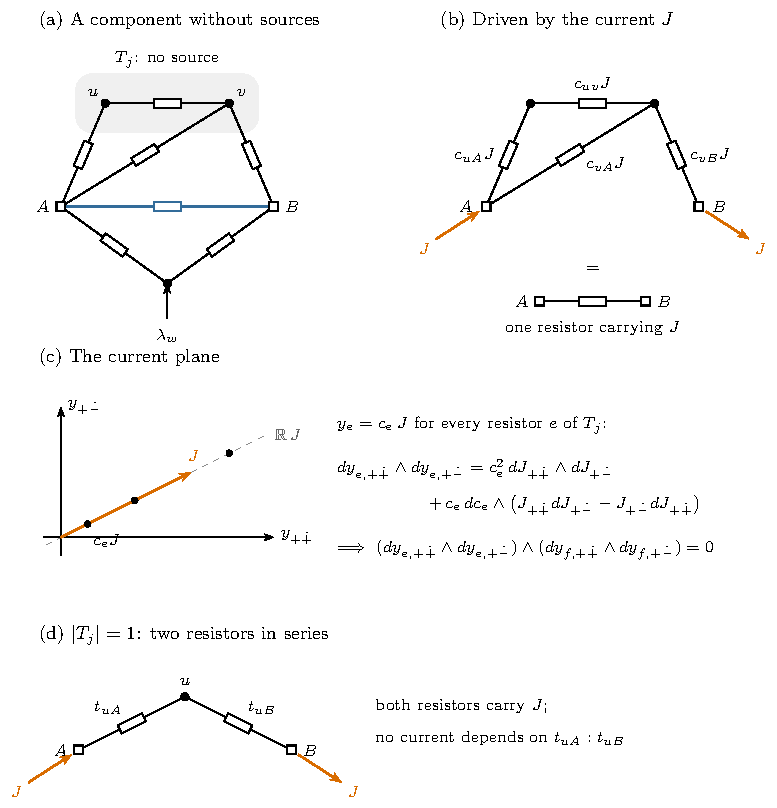
\includegraphics[width=0.82\linewidth]{figures/vec/figures-circuits-sourceless_component.pdf}
\caption{A component without sources. (a) A component $T_j$ with no injected current meets the rest of the circuit only at the insertions $A$ and $B$; here the rest is the marked resistor (blue) and a node fed by $\lambda_w$. (b) The current $J$ entering $T_j$ at $A$ leaves it at $B$, and every current of $T_j$ is $c_eJ$ with a real current-division ratio $c_e$: the component acts as one resistor carrying $J$. (c) All currents of $T_j$ lie on the line $\mathbb RJ$ of the current plane, so each of their area forms is \eqref{eq-sourceless-component}, and the product of two of them vanishes. (d) For $|T_j|=1$ the two resistors are in series, and no current depends on the ratio of their resistances.}
\label{fig-sourceless}
\end{figure}

Replace the source-free component by its effective resistor between $A,B$ and merge it with the marked resistor; call the resulting circuit $\Gamma^{\mathrm{red}}$. If $|T_j|=1$, its vertex $v$ has $\lambda_v=0$, and Theorem \ref{b-01142} gives

\begin{equation*}
\begin{aligned}
\mathcal I_\Gamma(\lambda;z)
&=\int_0^1dr_1\int_0^1dr_2\,
\underbrace{\left.r_2\lambda_{v,+}{}^{\dot a}
\frac{\partial}{\partial z_{AB}^{\mathrm{red},+\dot a}}\right|_{\lambda_v=0}}_{\text{zero current-area operator}}
\mathcal I_{\Gamma^{\mathrm{red}}}(\lambda;z^{\mathrm{red}})
=0.
\end{aligned}
\end{equation*}

If $|T_j|\ge2$, choose a spanning tree containing $AB$ and $|T_j|$ resistors of the component. There are $|T_j|$ complementary component resistors; for any two, $e,f$, \eqref{eq-sourceless-component} gives

\begin{equation*}
\begin{aligned}
&(dy_{e,+\dot+}\wedge dy_{e,+\dot-})
\wedge(dy_{f,+\dot+}\wedge dy_{f,+\dot-})\\
&=\Big[c_e^2dJ_{+\dot+}\wedge dJ_{+\dot-}
+c_e\,dc_e\wedge(J_{+\dot+}dJ_{+\dot-}-J_{+\dot-}dJ_{+\dot+})\Big]\\
&\quad\wedge\Big[c_f^2dJ_{+\dot+}\wedge dJ_{+\dot-}
+c_f\,dc_f\wedge(J_{+\dot+}dJ_{+\dot-}-J_{+\dot-}dJ_{+\dot+})\Big]=0,\\
&\mathcal I_\Gamma(\lambda;z)
=\underbrace{0}_{\text{current-area Jacobian of the component}}
\mathcal I_{\Gamma^{\mathrm{red}}}(\lambda;z^{\mathrm{red}})=0.
\end{aligned}
\end{equation*}

\emph{Trees.} If the internal resistors of $T_j$ close a loop, they number at least $|T_j|$; by \eqref{eq-1-20} they number exactly $|T_j|$, $T_j$ has no $\bar W$ node, and $|E_j|=|T_j|$. The $2|T_j|$ ends of the internal resistors and the $|T_j|$ spokes then wire all $3|T_j|$ terminals of its cubic nodes. No current is injected in $T_j$, and it becomes a component without sources, which gives zero. Every $T_j$ is therefore a tree, $|I_j|=|T_j|-1$, and \eqref{eq-1-20} gives at most one $\bar W$ node and $|E_j|=|T_j|+1$, which is \eqref{eq-1-19}.

\emph{Spokes and degrees.} Since $|E_j|=|T_j|+1$~and each node can be joined to each of $A$ and $B$ at most once, each component must have spokes to both $A$ and $B$.

\emph{Quadratic terms of $\bar W$.} A quadratic term of $\bar W$ is a node with two terminals, both wired by the previous step, so it injects no current. It is the only $\bar W$ node of its tree, whose $3(|T_j|-1)+2=3|T_j|-1$ terminals are then all wired by the $|T_j|-1$ internal resistors and the $|T_j|+1$ spokes. The tree carries no source, and the first step gives zero.~

A source at a vertex is supplied by its uncontracted fields. For cubic vertices the count is one; if $T_j$ contains a superpotential monomial,

\begin{equation*}
\begin{aligned}
\#(\text{uncontracted fields in }T_j)
&=3(|T_j|-1)+\deg\bar W-2(|T_j|-1)-(|T_j|+1)\\
&=\deg\bar W-2,\\
\#\{v\in T_j:\lambda_v\ne0\}
&\le\#(\text{uncontracted fields in }T_j)=\deg\bar W-2.
\end{aligned}
\end{equation*}

Thus the bound is one for cubic interactions, and is not uniformly one for arbitrary $\bar W$.\hfill\qedsymbol

\rthm{Proposition}{b-00366}{Cubic interactions have a starting point for the iteration: a vertex of degree two} \emph{Let every vertex of $\mathcal I$ be cubic, as are the gauge and matter vertices of \eqref{eq-B-10} together with a cubic $\bar W$. } \emph{In every tree $T_j$ of \eqref{eq-1-19}, exactly one vertex has degree two, and its uncontracted field is the only output field of $T_j$; all other vertices have degree three. } \emph{The tree degree of a vertex is its number of internal edges, and the number of spokes at a vertex of given tree degree is}
\begin{equation}\label{eq-product-local-spokes}
\begin{array}{c|cccc}
\text{tree degree}&0&1&2&3\\\hline
\text{spokes if }\deg_\Gamma v=3&\text{--}&2&1&0\\
\text{spokes if }\deg_\Gamma v=2&2&1&0&\text{--}
\end{array}
\end{equation}
\emph{and a vertex with two spokes is joined to both $A$ and $B$ (Figure~\ref{fig-forest-components}).}

\begin{figure}[H]
\centering
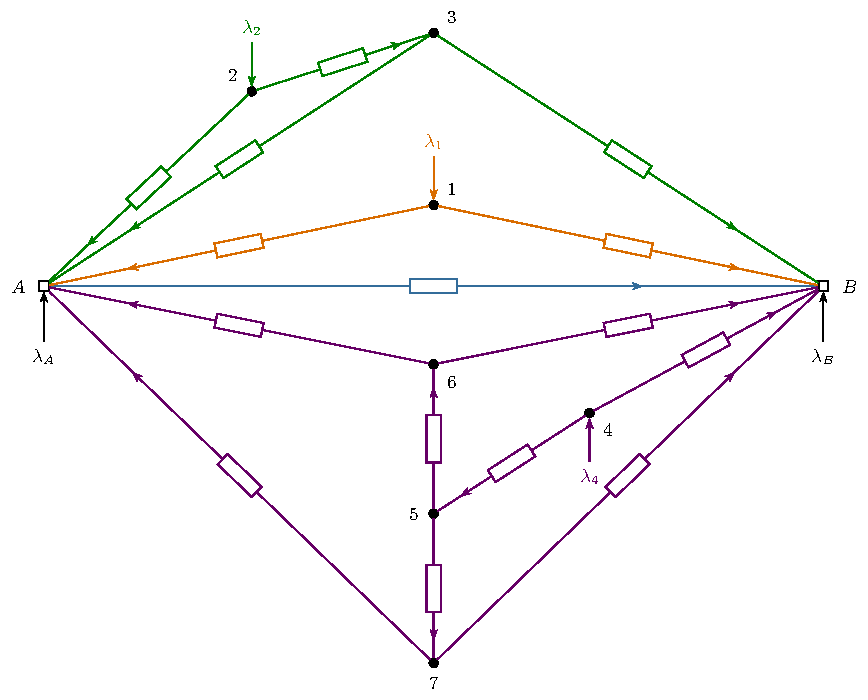
\includegraphics[width=0.92\linewidth]{figures/vec/figures-circuits-forest_components.pdf}
\caption{A seven-loop product graph with three trees, each in its own colour, between the insertions $A$ and $B$; the marked edge $AB$ is blue. Each tree has one more spoke than vertices, and its source enters at its only vertex of degree two: $1$, $2$ and $4$. Leaves of degree three are joined to both insertions, and the branching vertex $5$ has no spoke.}
\label{fig-forest-components}
\end{figure}

\emph{Proof.} A cubic node has three terminals. In $T_j$ the $|T_j|-1$ internal resistors wire $2(|T_j|-1)$ terminals and the $|T_j|+1$ spokes wire $|T_j|+1$ more, so the numbers of resistors at its nodes add up to
\begin{equation}\label{eq-product-degree-sum}
\sum_{v\in T_j}\deg_\Gamma v=2(|T_j|-1)+(|T_j|+1)=3|T_j|-1 .
\end{equation}

Every node has two or three resistors by Proposition~\ref{b-00355}, so exactly one node has two, and
\begin{equation}\label{eq-1-21}
\underbrace{3|T_j|}_{\text{terminals}}-\underbrace{2(|T_j|-1)}_{\text{internal resistor ends}}-\underbrace{(|T_j|+1)}_{\text{spokes}}=1
\end{equation}
terminal stays free, at that node: each tree carries a single source, injected at its node with two resistors.\hfill\qedsymbol

\subsubsection{Graphs of type \texorpdfstring{I$'$}{I'}}\label{sec-B-typeI}

\textbf{Definition.} A graph of type I$\prime$ is built from one edge by adding vertices joined to both endpoints of an existing edge \cite[Definition 4.12]{GWW}.

\rthm{Proposition}{b-01345}{} Let $\Gamma$ contain $AB$, interaction trees $T_j$, and at most one spoke per vertex to each insertion, with $|E_j|=|T_j|+1$ spokes. Then $\Gamma$ is of type I$\prime$ exactly when the endpoints of every internal edge share an insertion neighbour. For cubic vertices, each tree is then an arm with a common insertion neighbour, its source at one endpoint, and both insertion spokes at the other. For $n\ge3$, it is a spider exactly when all arms of length at least two share the same insertion neighbour.

\begin{proofbox}
\emph{Proof.}

Every edge of a type I$\prime$ graph lies in a triangle. A triangle containing an internal edge must meet an insertion, since the internal graph is a forest. Conversely, the common-neighbour condition gives each interaction vertex a spoke. If every leaf had two, a tree with $L\ge2$ leaves would have
\begin{equation*}
|E_j|\ge2L+(|T_j|-L)\ge|T_j|+2,
\end{equation*}
contrary to the hypothesis. A leaf with one spoke is removed by a series--parallel step. Induction proves the first assertion. For cubic vertices, a vertex of tree degree three has zero spokes by \eqref{eq-product-local-spokes}. Thus every tree is a path, and its common insertion propagates along the path. The spider condition says precisely that this insertion is shared by all nontrivial arms. $\square$
\end{proofbox}

Table~\ref{tab-product-census} gives the marked-graph census through seven loops, up to isomorphism fixing $A,B$. The fan and spider columns exclude the book.

{\small\renewcommand{\arraystretch}{1.25}\setlength{\tabcolsep}{4pt}
\begin{xltabular}{\linewidth}{@{}llllllll>{\raggedright\arraybackslash}X@{}}
\caption{Census of the marked graphs through seven loops, up to isomorphism fixing $A,B$. The fan and spider columns exclude the book.}\label{tab-product-census}\\
\toprule
$n$ & graphs & books & fans & spiders & type~I$'$, & not type~I$'$, & branching & $A\leftrightarrow B$\\
\midrule\endhead
 &  &  &  & ($\ge3$ arms) & not spiders & paths & trees & symmetric\\
1 & 1 & 1 & 0 & 0 & 0 & 0 & 0 & 1\\
2 & 3 & 1 & 2 & 0 & 0 & 0 & 0 & 1\\
3 & 8 & 1 & 4 & 0 & 0 & 3 & 0 & 2\\
4 & 23 & 1 & 6 & 2 & 1 & 11 & 2 & 3\\
5 & 65 & 1 & 6 & 6 & 3 & 38 & 11 & 5\\
6 & 194 & 1 & 8 & 12 & 8 & 112 & 53 & 8\\
7 & 576 & 1 & 8 & 20 & 16 & 313 & 218 & 14\\
\bottomrule
\end{xltabular}}

The final iteration of these forest diagrams requires star--triangle transformations and is more involved; it is carried out in Section~\ref{sec-forest-graphs}. Since the graphs have many different topologies, there is no unique way to derive the final result in one step. At low loop orders ($n\le2$), however, all these forest diagrams belong to the fan and spider kernels, which are computed exactly in Sections~\ref{sec-fans} and~\ref{sec-spiders}.

\subsection{Kernels of general product forests}\label{sec-forest-graphs}

As noted in Section~\ref{sec-dressed-definition}, spiders do not exhaust the graphs of the quantum product: other graphs (general forests) occur from three loops on and are the majority from four loops on, where the trees also begin to branch (Table~\ref{tab-product-census}). The series--parallel move of Theorem~\ref{b-01142} and the two star--triangle moves below reduce all of them.\footnote{From three loops on, some of these graphs are Laman graphs not of type~I$'$ \cite[Definition 4.12]{GWW}: in the three-loop graph with edges $12,13,2A,2B,3A,3B,AB$, the only degree-two vertex, $1$, has neighbours that are not joined. These reductions therefore reach beyond the recursion of \cite[Theorem 4.13]{GWW}.}

The reduction of each tree in the forest can be done independently.

\subsubsection{Star--triangle moves as kernel operators}

As for the series--parallel move, each move becomes an operator on the reduced kernel; in successive moves, derivatives act on the entire expression to their right.

\rthm{Theorem}{b-01159}{Star--triangle, the first case: two edges present} In a Laman circuit, let $v$ have degree three, neighbours $u,w,x$, and source $\lambda_v$. Assume $ux,wx$ are present and $uw$ is absent. Let $r_1,r_2$ be the old $ux,wx$ current fractions. The reduction removes one vertex, two edges, and one loop, preserving the Laman condition.

For $\lambda_v=0$, the operator is \eqref{eq-kernel-star-triangle}; the complete sourced version~\eqref{local-B-sourced-operator} is given in Section~\ref{sources-at-a-trivalent-vertex}.
\begin{equation}\label{eq-kernel-star-triangle}
\begin{aligned}
\mathcal I_\Gamma(\lambda;z)
={}&\int_0^1dr_1\int_0^1dr_2\;
\underbrace{-r_1r_2
\frac{\partial}{\partial z_{ux}^{\mathrm{red},+\dot a}}
\frac{\partial}{\partial z_{wx,\dot a}^{\mathrm{red},+}}}_{\text{local current Jacobian}}
\mathcal I_{\Gamma^{\mathrm{red}}}(\lambda;z^{\mathrm{red}}).
\end{aligned}
\end{equation}
\begin{equation*}
\begin{aligned}
z_{uw}^{\mathrm{red}}&=z_{vw}-z_{vu},\\
z_{ux}^{\mathrm{red}}&=r_1z_{ux}+(1-r_1)(z_{vx}-z_{vu}),\\
z_{wx}^{\mathrm{red}}&=r_2z_{wx}+(1-r_2)(z_{vx}-z_{vw}),\\
z_e^{\mathrm{red}}&=z_e\quad(e\ne uw,ux,wx).
\end{aligned}
\end{equation*}

\begin{figure}[H]
\centering
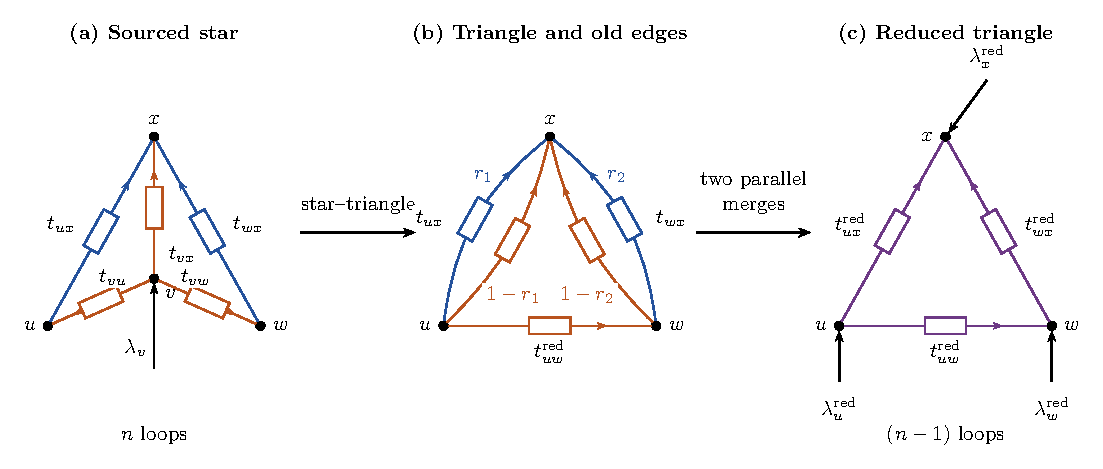
\includegraphics[width=0.96\linewidth]{figures/vec/b3-star-triangle-sourced-resistors-20261107.pdf}
\caption{Sourced star--triangle reduction. The source at $v$ is transferred to $u,w,x$; the blue and orange labels are fractions of the final merged currents.}
\label{local-31f8a28c-43da-41d0-98eb-cc09a3412cdf}
\end{figure}

\begin{proofbox}
\textbf{Proof for $\lambda_v=0$.} The star--triangle change \cite[Lemma 2.4.23]{Panzer} and the two merges give
\begin{equation*}
\begin{gathered}
t_{uw}^{\mathrm{red}}
=t_{vu}+t_{vw}+\frac{t_{vu}t_{vw}}{t_{vx}},\\
\frac1{t_{ux}^{\mathrm{red}}}
=\frac1{t_{ux}}+
\frac{t_{vw}}{t_{vu}t_{vw}+t_{vw}t_{vx}+t_{vx}t_{vu}},\\
\frac1{t_{wx}^{\mathrm{red}}}
=\frac1{t_{wx}}+
\frac{t_{vu}}{t_{vu}t_{vw}+t_{vw}t_{vx}+t_{vx}t_{vu}},\\
r_1=\frac{t_{ux}^{\mathrm{red}}}{t_{ux}},\qquad
r_2=\frac{t_{wx}^{\mathrm{red}}}{t_{wx}}.
\end{gathered}
\end{equation*}

The sign of this resistance change fixes the current-form orientation:
\begin{equation*}
\operatorname{sgn}\det
\frac{\partial(t_{vu},t_{vw},t_{vx},t_{ux},t_{wx})}
{\partial(r_1,r_2,t_{uw}^{\mathrm{red}},t_{ux}^{\mathrm{red}},t_{wx}^{\mathrm{red}})}
=-1.
\end{equation*}
\begin{equation}\label{b-01166}
\begin{aligned}
y_{vu}&=-y_{uw}^{\mathrm{red}}-(1-r_1)y_{ux}^{\mathrm{red}},\\
y_{vw}&=y_{uw}^{\mathrm{red}}-(1-r_2)y_{wx}^{\mathrm{red}},\\
y_{vx}&=(1-r_1)y_{ux}^{\mathrm{red}}+(1-r_2)y_{wx}^{\mathrm{red}},\\
y_{ux}&=r_1y_{ux}^{\mathrm{red}},\qquad y_{wx}=r_2y_{wx}^{\mathrm{red}}.
\end{aligned}
\end{equation}

These currents give the stated displacement substitutions.

Choose a reduced spanning tree containing $ux,wx$; conservation at fixed $\lambda$ makes $d(y_{ux,+\dot a}^{\mathrm{red}}+y_{uw,+\dot a}^{\mathrm{red}})$ and $d(y_{wx,+\dot a}^{\mathrm{red}}-y_{uw,+\dot a}^{\mathrm{red}})$ linear combinations of the other retained loop-current differentials; $\equiv$ denotes equality modulo those differentials.
\begin{equation*}
\begin{aligned}
dy_{ux,+\dot a}
&=y_{ux,+\dot a}^{\mathrm{red}}dr_1-r_1dy_{uw,+\dot a}^{\mathrm{red}}
+r_1d\!\left(y_{ux,+\dot a}^{\mathrm{red}}+y_{uw,+\dot a}^{\mathrm{red}}\right),\\
dy_{wx,+\dot a}
&=y_{wx,+\dot a}^{\mathrm{red}}dr_2+r_2dy_{uw,+\dot a}^{\mathrm{red}}
+r_2d\!\left(y_{wx,+\dot a}^{\mathrm{red}}-y_{uw,+\dot a}^{\mathrm{red}}\right).
\end{aligned}
\end{equation*}
\begin{equation*}
\begin{aligned}
&(-dy_{ux,+\dot+}\wedge dy_{ux,+\dot-})\wedge
(-dy_{wx,+\dot+}\wedge dy_{wx,+\dot-})\\
&=\frac14\Bigl[y_{ux,+\dot a}^{\mathrm{red}}dr_1-r_1dy_{uw,+\dot a}^{\mathrm{red}}
+r_1d\!\left(y_{ux,+\dot a}^{\mathrm{red}}+y_{uw,+\dot a}^{\mathrm{red}}\right)\Bigr]\\
&\quad\wedge\Bigl[y_{ux,+}^{\mathrm{red}}{}^{\dot a}dr_1-r_1dy_{uw,+}^{\mathrm{red}}{}^{\dot a}
+r_1d\!\left(y_{ux,+}^{\mathrm{red}}{}^{\dot a}+y_{uw,+}^{\mathrm{red}}{}^{\dot a}\right)\Bigr]\\
&\quad\wedge\Bigl[y_{wx,+\dot b}^{\mathrm{red}}dr_2+r_2dy_{uw,+\dot b}^{\mathrm{red}}
+r_2d\!\left(y_{wx,+\dot b}^{\mathrm{red}}-y_{uw,+\dot b}^{\mathrm{red}}\right)\Bigr]\\
&\quad\wedge\Bigl[y_{wx,+}^{\mathrm{red}}{}^{\dot b}dr_2+r_2dy_{uw,+}^{\mathrm{red}}{}^{\dot b}
+r_2d\!\left(y_{wx,+}^{\mathrm{red}}{}^{\dot b}-y_{uw,+}^{\mathrm{red}}{}^{\dot b}\right)\Bigr]\\
&\equiv-r_1r_2(y_{ux,+\dot a}^{\mathrm{red}}y_{wx,+}^{\mathrm{red}}{}^{\dot a})
dr_1\wedge dr_2\wedge
(-dy_{uw,+\dot+}^{\mathrm{red}}\wedge dy_{uw,+\dot-}^{\mathrm{red}}).
\end{aligned}
\end{equation*}

Replacing the paired currents by the two displacement derivatives proves \eqref{eq-kernel-star-triangle}. $\square$
\end{proofbox}

\rthm{Theorem}{b-01173}{Star--triangle, the second case: two star--triangle reductions at a time} In a Laman circuit, let $v_1,v_2$ be source-free degree-three vertices joined to $u,A,B$, with $AB$ present and $uA,uB$ absent. The conductance fractions contributed by the $v_1$ star to $uA,uB$ are $r_1,r_2$; those contributed by the $v_2$ star are $1-r_1,1-r_2$. The fractions on $AB$ contributed by $v_1$, $v_2$ and the old edge are $r_3,r_4,1-r_3-r_4$. The reduction removes two vertices, four edges and two loops, preserving the Laman condition.

\begin{figure}[H]
\centering
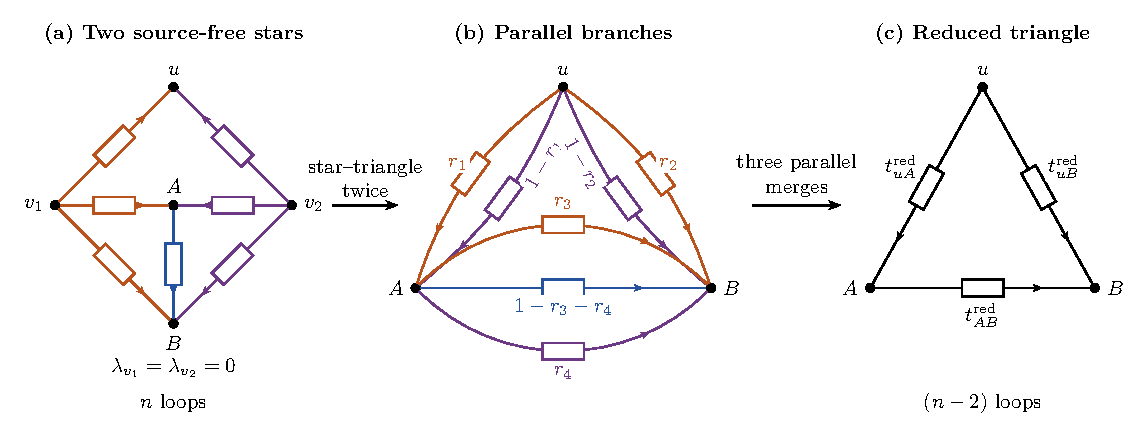
\includegraphics[width=0.96\linewidth]{figures/vec/b3-two-stars-resistors-20261107.pdf}
\caption{Two source-free stars reduce to a triangle by two star--triangle moves and three parallel merges. Orange and purple branches come from $v_1$ and $v_2$; blue is the old $AB$ edge. The labels in the middle panel are fractions of the final merged currents.}
\label{local-d68f49d7-1a60-45ce-ab33-5f20a940d12e}
\end{figure}

\begin{equation}\label{eq-kernel-two-leaves}
\begin{aligned}
\mathcal I_\Gamma(\lambda;z)
={}&\int_0^1dr_1\int_0^1dr_2
\int_{\substack{r_3>0,\ r_4>0\\r_3+r_4<1}}dr_3\,dr_4\\
&\times(r_1-r_2)(1-r_3-r_4)\\
&\times\frac{\partial}{\partial z_{uA}^{\mathrm{red},+\dot a}}
\frac{\partial}{\partial z_{AB,\dot a}^{\mathrm{red},+}}
\frac{\partial}{\partial z_{uB}^{\mathrm{red},+\dot c}}
\frac{\partial}{\partial z_{AB,\dot c}^{\mathrm{red},+}}
\mathcal I_{\Gamma^{\mathrm{red}}}(\lambda;z^{\mathrm{red}}).
\end{aligned}
\end{equation}
\begin{equation*}
\begin{aligned}
z_{uA}^{\mathrm{red}}&=r_1(z_{v_1A}-z_{v_1u})+(1-r_1)(z_{v_2A}-z_{v_2u}),\\
z_{uB}^{\mathrm{red}}&=r_2(z_{v_1B}-z_{v_1u})+(1-r_2)(z_{v_2B}-z_{v_2u}),\\
z_{AB}^{\mathrm{red}}&=(1-r_3-r_4)z_{AB}+r_3(z_{v_1B}-z_{v_1A})+r_4(z_{v_2B}-z_{v_2A}),\\
z_e^{\mathrm{red}}&=z_e\quad(e\ne uA,uB,AB).
\end{aligned}
\end{equation*}

\begin{proofbox}
\textbf{Proof.} The two star--triangle changes and three merges preserve orientation.

The branch resistances are
\begin{equation*}
\begin{aligned}
\frac{t_{uA}^{\mathrm{red}}}{r_1}
&=t_{v_1u}+t_{v_1A}+\frac{t_{v_1u}t_{v_1A}}{t_{v_1B}},\\
\frac{t_{uA}^{\mathrm{red}}}{1-r_1}
&=t_{v_2u}+t_{v_2A}+\frac{t_{v_2u}t_{v_2A}}{t_{v_2B}},\\[2pt]
\frac{t_{uB}^{\mathrm{red}}}{r_2}
&=t_{v_1u}+t_{v_1B}+\frac{t_{v_1u}t_{v_1B}}{t_{v_1A}},\\
\frac{t_{uB}^{\mathrm{red}}}{1-r_2}
&=t_{v_2u}+t_{v_2B}+\frac{t_{v_2u}t_{v_2B}}{t_{v_2A}},\\[2pt]
\frac{t_{AB}^{\mathrm{red}}}{r_3}
&=t_{v_1A}+t_{v_1B}+\frac{t_{v_1A}t_{v_1B}}{t_{v_1u}},\\
\frac{t_{AB}^{\mathrm{red}}}{r_4}
&=t_{v_2A}+t_{v_2B}+\frac{t_{v_2A}t_{v_2B}}{t_{v_2u}},\\
\frac{t_{AB}^{\mathrm{red}}}{1-r_3-r_4}&=t_{AB}.
\end{aligned}
\end{equation*}
\begin{equation}\label{b-01180}
\begin{aligned}
y_{v_1u}&=-r_1y_{uA}^{\mathrm{red}}-r_2y_{uB}^{\mathrm{red}},&
y_{v_2u}&=-(1-r_1)y_{uA}^{\mathrm{red}}-(1-r_2)y_{uB}^{\mathrm{red}},\\
y_{v_1A}&=r_1y_{uA}^{\mathrm{red}}-r_3y_{AB}^{\mathrm{red}},&
y_{v_2A}&=(1-r_1)y_{uA}^{\mathrm{red}}-r_4y_{AB}^{\mathrm{red}},\\
y_{v_1B}&=r_2y_{uB}^{\mathrm{red}}+r_3y_{AB}^{\mathrm{red}},&
y_{v_2B}&=(1-r_2)y_{uB}^{\mathrm{red}}+r_4y_{AB}^{\mathrm{red}},\\
y_{AB}&=(1-r_3-r_4)y_{AB}^{\mathrm{red}}.
\end{aligned}
\end{equation}

Choose a reduced spanning tree containing $uA,uB$. At fixed $\lambda$, conservation makes $d(y_{uA,+\dot a}^{\mathrm{red}}-y_{AB,+\dot a}^{\mathrm{red}})$ and $d(y_{uB,+\dot a}^{\mathrm{red}}+y_{AB,+\dot a}^{\mathrm{red}})$ linear combinations of the other reduced chord-current differentials. The determinant is
\begin{equation*}
\begin{aligned}
&\det\frac{\partial(y_{AB,+\dot+},y_{AB,+\dot-},y_{v_1B,+\dot+},y_{v_1B,+\dot-},y_{v_2A,+\dot+},y_{v_2A,+\dot-})}
{\partial(r_1,r_2,r_3,r_4,y_{AB,+\dot+}^{\mathrm{red}},y_{AB,+\dot-}^{\mathrm{red}})}\\
&=(r_1-r_2)(1-r_3-r_4)
(y_{uA,+\dot a}^{\mathrm{red}}y_{AB,+}^{\mathrm{red}}{}^{\dot a})
(y_{uB,+\dot b}^{\mathrm{red}}y_{AB,+}^{\mathrm{red}}{}^{\dot b}).
\end{aligned}
\end{equation*}
\begin{equation*}
\begin{aligned}
dy_{AB,+\dot a}
&=(1-r_3-r_4)dy_{AB,+\dot a}^{\mathrm{red}}
-y_{AB,+\dot a}^{\mathrm{red}}(dr_3+dr_4),\\
dy_{v_1B,+\dot a}
&=y_{uB,+\dot a}^{\mathrm{red}}dr_2+y_{AB,+\dot a}^{\mathrm{red}}dr_3
+(r_3-r_2)dy_{AB,+\dot a}^{\mathrm{red}}\\
&\quad+r_2d\!\left(y_{uB,+\dot a}^{\mathrm{red}}+y_{AB,+\dot a}^{\mathrm{red}}\right),\\
dy_{v_2A,+\dot a}
&=-y_{uA,+\dot a}^{\mathrm{red}}dr_1-y_{AB,+\dot a}^{\mathrm{red}}dr_4
+(1-r_1-r_4)dy_{AB,+\dot a}^{\mathrm{red}}\\
&\quad+(1-r_1)d\!\left(y_{uA,+\dot a}^{\mathrm{red}}-y_{AB,+\dot a}^{\mathrm{red}}\right).
\end{aligned}
\end{equation*}

In the following wedge products, $\equiv$ omits terms containing $dy_{e,+\dot+}^{\mathrm{red}}$ or $dy_{e,+\dot-}^{\mathrm{red}}$, where $e\ne AB$ lies outside the chosen reduced spanning tree. They vanish after wedging with the area forms of all those remaining chord currents.
\begin{equation*}
\begin{aligned}
&dy_{AB,+\dot+}\wedge dy_{AB,+\dot-}\\
&=(1-r_3-r_4)^2
 dy_{AB,+\dot+}^{\mathrm{red}}\wedge dy_{AB,+\dot-}^{\mathrm{red}}\\
&\quad-(1-r_3-r_4)(dr_3+dr_4)\wedge
\bigl(y_{AB,+\dot a}^{\mathrm{red}}dy_{AB,+}^{\mathrm{red}}{}^{\dot a}\bigr).
\end{aligned}
\end{equation*}
\begin{equation*}
\begin{aligned}
&dy_{v_1B,+\dot+}\wedge dy_{v_1B,+\dot-}\\
&\equiv
\bigl(y_{uB,+\dot a}^{\mathrm{red}}y_{AB,+}^{\mathrm{red}}{}^{\dot a}\bigr)
 dr_2\wedge dr_3\\
&\quad+(r_3-r_2)dr_2\wedge
\bigl(y_{uB,+\dot a}^{\mathrm{red}}dy_{AB,+}^{\mathrm{red}}{}^{\dot a}\bigr)\\
&\quad+(r_3-r_2)dr_3\wedge
\bigl(y_{AB,+\dot a}^{\mathrm{red}}dy_{AB,+}^{\mathrm{red}}{}^{\dot a}\bigr)\\
&\quad+(r_3-r_2)^2
 dy_{AB,+\dot+}^{\mathrm{red}}\wedge dy_{AB,+\dot-}^{\mathrm{red}}.
\end{aligned}
\end{equation*}
\begin{equation*}
\begin{aligned}
&dy_{v_2A,+\dot+}\wedge dy_{v_2A,+\dot-}\\
&\equiv
\bigl(y_{uA,+\dot a}^{\mathrm{red}}y_{AB,+}^{\mathrm{red}}{}^{\dot a}\bigr)
 dr_1\wedge dr_4\\
&\quad-(1-r_1-r_4)dr_1\wedge
\bigl(y_{uA,+\dot a}^{\mathrm{red}}dy_{AB,+}^{\mathrm{red}}{}^{\dot a}\bigr)\\
&\quad-(1-r_1-r_4)dr_4\wedge
\bigl(y_{AB,+\dot a}^{\mathrm{red}}dy_{AB,+}^{\mathrm{red}}{}^{\dot a}\bigr)\\
&\quad+(1-r_1-r_4)^2
 dy_{AB,+\dot+}^{\mathrm{red}}\wedge dy_{AB,+\dot-}^{\mathrm{red}}.
\end{aligned}
\end{equation*}
\begin{equation*}
\begin{aligned}
&dy_{AB,+\dot+}\wedge dy_{AB,+\dot-}
\wedge dy_{v_1B,+\dot+}\wedge dy_{v_1B,+\dot-}
\wedge dy_{v_2A,+\dot+}\wedge dy_{v_2A,+\dot-}\\
&\equiv\Bigl[(1-r_3-r_4)^2
 -(1-r_3-r_4)(1-r_1-r_4)\\
&\hspace{42mm}+(1-r_3-r_4)(r_3-r_2)\Bigr]\\
&\quad\times
\bigl(y_{uA,+\dot a}^{\mathrm{red}}y_{AB,+}^{\mathrm{red}}{}^{\dot a}\bigr)
\bigl(y_{uB,+\dot b}^{\mathrm{red}}y_{AB,+}^{\mathrm{red}}{}^{\dot b}\bigr)\\
&\quad\times dr_1\wedge dr_2\wedge dr_3\wedge dr_4
\wedge dy_{AB,+\dot+}^{\mathrm{red}}\wedge dy_{AB,+\dot-}^{\mathrm{red}}\\
&=(r_1-r_2)(1-r_3-r_4)
\bigl(y_{uA,+\dot a}^{\mathrm{red}}y_{AB,+}^{\mathrm{red}}{}^{\dot a}\bigr)
\bigl(y_{uB,+\dot b}^{\mathrm{red}}y_{AB,+}^{\mathrm{red}}{}^{\dot b}\bigr)\\
&\quad\times dr_1\wedge dr_2\wedge dr_3\wedge dr_4
\wedge dy_{AB,+\dot+}^{\mathrm{red}}\wedge dy_{AB,+\dot-}^{\mathrm{red}},\\
&\quad\text{modulo }dy_{e,+\dot+}^{\mathrm{red}},\,dy_{e,+\dot-}^{\mathrm{red}}
\quad(e\ne AB\text{ a reduced chord}).
\end{aligned}
\end{equation*}

The three loop-area minus signs reduce to the one on the retained loop. The four displacement derivatives insert the displayed current product. $\square$
\end{proofbox}

\subsubsection{Cubic product forests}\label{sec-B-general-forests}

\rthm{Definition}{local-a46302f1-f575-4089-89c2-a258e201a5ce}{Rooted interaction trees} Root a cubic interaction tree at its unique vertex of full graph degree two. The parent of a non-root vertex $v$ is its neighbour on the path to the root; the other tree neighbours are its children, and vertices with the same parent are siblings. A spoke at a vertex $u$ is an edge $uA$ or $uB$.

\emph{The subtree of a vertex consists of the vertices whose path to the root passes through it.}

\begin{figure}[H]
\centering
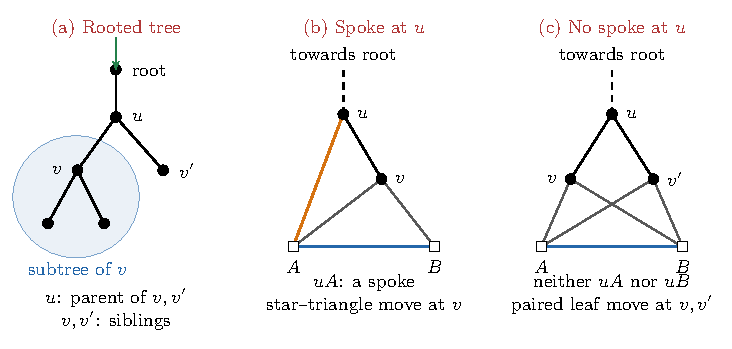
\includegraphics[width=0.78\linewidth]{figures/vec/ch6-rooted-tree-neighborhoods-20261102.pdf}
\caption{Rooted-tree terminology and the two reduction neighborhoods. (a) The shaded subtree contains $v$ and its descendants; $u$ is the parent of $v,v'$, which are siblings. (b) The edge $uA$ is a spoke; after the descendants of $v$ are removed, a star--triangle move removes $v$. (c) The parent $u$ has no spoke; after both descendant subtrees are removed, $v,v'$ are eliminated together. Dashed edges continue towards the root; the blue edge is $AB$.}
\label{fig-rooted-tree-neighborhoods}
\end{figure}

\rthm{Proposition}{b-00405}{Kernels of cubic product forests} \emph{Let $\Gamma$ be a nonzero marked graph of the quantum product with cubic interaction vertices (Proposition~\ref{b-00366}), and root each tree at its vertex of degree two, its only source. }

(i) \emph{If $\Gamma$ is of type~I$'$, series--parallel moves (Theorem~\ref{b-01142}) along each arm reduce it to the marked resistor, which then carries}
\begin{equation}\label{eq-product-typeI-current}
y^{\mathrm{red}}_{AB,+\dot a}
=\lambda_{A,+\dot a}
+\sum_{\text{arms at }B}\left(\prod_{k=1}^{\ell_i}r_{i,2k-1}\right)\lambda_{v_{i,1},+\dot a}
+\sum_{\text{arms at }A}\left(1-\prod_{k=1}^{\ell_i}r_{i,2k-1}\right)\lambda_{v_{i,1},+\dot a}.
\end{equation}
\emph{summed over the arms wired to $B$ and to $A$. The reduction is similar to that in Figure~\ref{fig-spider-reduction}, the reduction of spiders.}

(ii) \emph{Every $\Gamma$ is reduced to the marked resistor by removing each vertex after all the vertices of its subtree. } \emph{A source-free vertex is removed by a star--triangle move (Theorem~\ref{b-01159}) when its tree neighbor towards the root has a spoke, and together with its sibling (Theorem~\ref{b-01173}) when that neighbor has none; the root is removed last, by a series--parallel move (Figure~\ref{fig-sum-forest}).}

(iii) \emph{The kernel of $\Gamma$ is an integral over $2n$ coordinates, ranging over intervals and simplices, of a polynomial density times the exponential of polynomial currents (the displacements), and each Taylor coefficient in the displacements is a finite sum of the moments of unit intervals and standard simplices $\Delta$,}
\begin{equation}\label{eq-Dirichlet}
\int_{\substack{r_j>0\\\sum_{\substack{1\le j\le\dim\Delta\\\mathrm{coordinates}}}r_j<1}}
\prod_{j=1}^{\dim\Delta}(r_j^{k_j}\,dr_j)
=\frac{\prod_{j=1}^{\dim\Delta}k_j!}
{\left(\dim\Delta+\sum_{\substack{1\le j\le\dim\Delta\\\mathrm{coordinates}}}k_j\right)!}.
\end{equation}
\emph{(The essential point is that no ``spanning tree denominators'' remain and the calculation is polynomial.)}

\begin{figure}[H]
\centering
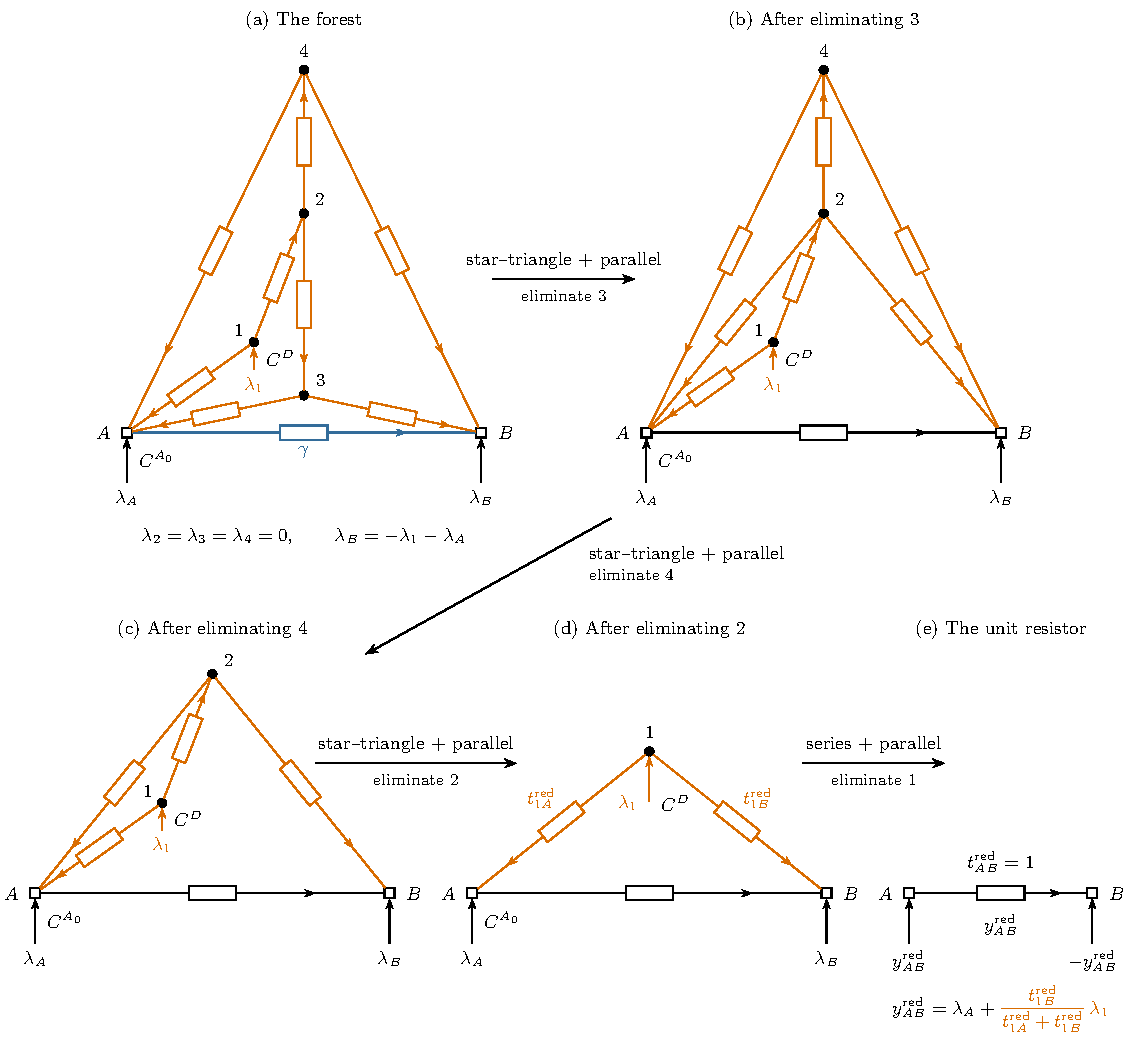
\includegraphics[width=0.96\linewidth]{figures/vec/figures-circuits-forest_star_triangle_v3.pdf}
\caption{Reduction of a four-loop product forest with tree edges $12,23,24$, spokes $1A,3A,3B,4A,4B$ and the marked edge $AB$ in blue. Star--triangle moves remove the source-free vertices $3$, $4$ and $2$, one per step (the pair $3,4$ is the paired move of Theorem~\ref{b-01173}, drawn in two steps), and the new resistors merge in parallel with existing ones; the root $1$, carrying $\lambda_1$, is removed last by a series step and a parallel merge with $AB$.}
\label{fig-sum-forest}
\end{figure}

\emph{Proof.} (i) By Proposition~\ref{b-01345}, every tree is an arm $v_{i,1}-\cdots-v_{i,\ell_i}$ whose nodes are all wired to one insertion, with the source at $v_{i,1}$ and a resistor from $v_{i,\ell_i}$ to each insertion. On an arm wired to $B$, the two resistors of $v_{i,1}$ end at $v_{i,2}$ and $B$, which are joined, so Theorem~\ref{b-01142} removes $v_{i,1}$ and passes the fraction $r_{i,1}$ of its source to $v_{i,2}$, which then has two resistors in turn. The source that reaches the last node of the arm is $\prod_kr_{i,2k-1}\lambda_{v_{i,1}}$, and the last move passes it to $A$ across the marked resistor, as for the spider \eqref{eq-spider-reduced}. On an arm wired to $A$ the same moves run with $A$ and $B$ exchanged, and the fraction of the source that reaches $A$ is $1-\prod_kr_{i,2k-1}$. Conservation at $A$ gives \eqref{eq-product-typeI-current}.

(ii) A source-free vertex $v$ whose subtree is gone has three resistors, to its tree neighbour $u$ towards the root, to $A$ and to $B$: its own spokes and the sides left by the moves at its children, merged in parallel. If $u$ has a spoke, to $X\in\{A,B\}$, two sides of the triangle that replaces $v$, namely $uX$ and $AB$, merge with resistors already there, and Theorem~\ref{b-01159} removes $v$. See Figure~\ref{fig-forest-three-loop}(a). If $u$ has none, then by \eqref{eq-product-local-spokes} $u$ has a second child $v'$, and once the subtree of $v'$ is gone, Theorem~\ref{b-01173} removes $v$ and $v'$ together. (The two star--triangle transformations at $v$ and $v'$ are performed together.) In both cases $u$ is then wired to $A$ and to $B$. The root, once its subtree is gone, has two resistors, to $A$ and to $B$, which the marked resistor joins, and Theorem~\ref{b-01142} removes it across $AB$.

(iii) Each move integrates the kernel of the smaller circuit over its ratios with a polynomial (not rational) factor. The currents of the larger circuit are linear in those of the smaller one with polynomial coefficients, and the series--parallel moves pass sources on with the weights $r_1$ and $1-r_1$. A move removes one loop with two coordinates, or two loops with four, so the coordinates number $2n$. Expanding the exponential, every Taylor coefficient is a polynomial integral over products of intervals and simplices, a finite sum of \eqref{eq-Dirichlet}.~\hfill\qedsymbol

\begin{figure}[H]
\centering
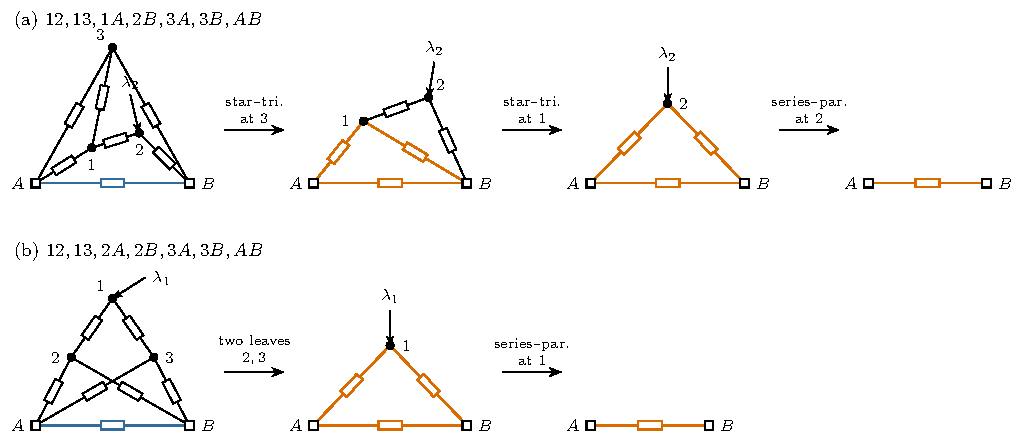
\includegraphics[width=0.96\linewidth]{figures/vec/figures-circuits-forest_three_loop.pdf}
\caption{The three-loop graphs not of type~I$'$, up to the exchange of $A$ and $B$, reduced as in Proposition~\ref{b-00405}(ii); orange: the resistors created or merged by the preceding move, blue: the marked resistor. (a) Star--triangle moves (Theorem~\ref{b-01159}) at $3$ and at $1$, then a series--parallel move (Theorem~\ref{b-01142}) at the root $2$. (b) The leaves $2,3$ hang from the root $1$, which has no spoke, and are removed together (Theorem~\ref{b-01173}); the root is removed last.}
\label{fig-forest-three-loop}
\end{figure}

In terms of kernel operators, root each cubic interaction tree at its unique source and process its descendants first. A source-free leaf uses \eqref{eq-kernel-star-triangle} when its parent has an insertion spoke; two sibling leaves use \eqref{eq-kernel-two-leaves}; a remaining degree-two source uses \eqref{eq-kernel-series-parallel}. Keep applying the operator to the smaller kernel inside the integral, stop at the final triangle, and insert its known one-loop kernel.

\rthm{Example}{local-f9b9d0e6-6c56-430a-826a-b94fe7879755}{Figure~\ref{fig-forest-three-loop}(a)} For $\lambda_1=\lambda_3=0$ and $\lambda_B=-\lambda_A-\lambda_2$, apply \eqref{eq-kernel-star-triangle} at $3$ and $1$, then \eqref{eq-kernel-series-parallel} at $2$. The successive ordered edge lists are
\begin{equation*}
\begin{aligned}
I&=(12,13,1A,2B,3A,3B,AB),\\
(\Gamma^{\mathrm{red}})_1&=(1B,12,1A,2B,AB),\\
(\Gamma^{\mathrm{red\,red}})_1&=(2A,2B,AB),\\
(\Gamma^{\mathrm{red\,red\,red}})_1&=(AB).
\end{aligned}
\end{equation*}

Use $r_1,r_2$ for the first star--triangle move, $r_3,r_4$ for the second, and $r_5,r_6$ for the series--parallel move, all in $(0,1)$. Their displacement substitutions and source transfer are
\begin{equation*}
\begin{aligned}
z^{\mathrm{red}}_{1B}&=z_{13}+z_{3B},
&z^{\mathrm{red}}_{1A}&=r_1z_{1A}+(1-r_1)(z_{13}+z_{3A}),\\
z^{\mathrm{red}}_{AB}&=r_2z_{AB}+(1-r_2)(z_{3B}-z_{3A}),
&z^{\mathrm{red}}_{12}&=z_{12},\quad z^{\mathrm{red}}_{2B}=z_{2B},\\
z^{\mathrm{red\,red}}_{2A}&=z^{\mathrm{red}}_{1A}-z_{12},
&z^{\mathrm{red\,red}}_{2B}&=r_3z_{2B}+(1-r_3)(z^{\mathrm{red}}_{1B}-z_{12}),\\
z^{\mathrm{red\,red}}_{AB}&=r_4z^{\mathrm{red}}_{AB}
+(1-r_4)(z^{\mathrm{red}}_{1B}-z^{\mathrm{red}}_{1A}),\\
z^{\mathrm{red\,red\,red}}_{AB}&=r_6z^{\mathrm{red\,red}}_{AB}
+(1-r_6)(z^{\mathrm{red\,red}}_{2B}-z^{\mathrm{red\,red}}_{2A}),\\
\lambda_A^{\mathrm{red\,red\,red}}&=\lambda_A+r_5\lambda_2,
&\lambda_B^{\mathrm{red\,red\,red}}&=\lambda_B+(1-r_5)\lambda_2.
\end{aligned}
\end{equation*}

Derivatives act before these substitutions. With $z_{BA}^{\mathrm{red}}=-z_{AB}^{\mathrm{red}}$, the chain rule gives
\begin{equation*}
\begin{aligned}
-
\frac{\partial}{\partial z_{1A}^{\mathrm{red},+\dot a}}
\frac{\partial}{\partial z_{BA,\dot a}^{\mathrm{red},+}}
&=-
\underbrace{\left(
\frac{\partial}{\partial z_{2A}^{\mathrm{red\,red},+\dot a}}
-(1-r_4)\frac{\partial}{\partial z_{AB}^{\mathrm{red\,red},+\dot a}}
\right)}_{\text{displacement Jacobian}}
\underbrace{\left(-r_4\frac{\partial}{\partial z_{AB,\dot a}^{\mathrm{red\,red},+}}\right)}_{\text{displacement Jacobian}}\\
&=r_4
\frac{\partial}{\partial z_{2A}^{\mathrm{red\,red},+\dot a}}
\frac{\partial}{\partial z_{AB,\dot a}^{\mathrm{red\,red},+}}.
\end{aligned}
\end{equation*}
\begin{equation*}
\begin{aligned}
\mathcal I_\Gamma(\lambda;z)
={}&-\int_{(0,1)^2}dr_1\,dr_2\,r_1r_2\,
\frac{\partial}{\partial z_{1A}^{\mathrm{red},+\dot a}}
\frac{\partial}{\partial z_{BA,\dot a}^{\mathrm{red},+}}
\underbrace{\mathcal I_{\Gamma^{\mathrm{red}}}
(\lambda;z^{\mathrm{red}})}_{\text{two loops}}\\
={}&-\int_{(0,1)^4}\prod_{j=1}^4dr_j\,r_1r_2r_3r_4^2\,\\
&\quad\times
\frac{\partial}{\partial z_{2A}^{\mathrm{red\,red},+\dot a}}
\frac{\partial}{\partial z_{AB,\dot a}^{\mathrm{red\,red},+}}
\frac{\partial}{\partial z_{2B}^{\mathrm{red\,red},+\dot c}}
\frac{\partial}{\partial z_{AB,\dot c}^{\mathrm{red\,red},+}}
\\
&\quad\times\underbrace{\mathcal I_{\Gamma^{\mathrm{red\,red}}}
(\lambda;z^{\mathrm{red\,red}})}_{\text{one loop}}\\
={}&-\bigl(\lambda_{2,+\dot a}\lambda_{A,+}{}^{\dot a}\bigr)^3
\int_{(0,1)^6}\prod_{j=1}^6dr_j\,
 r_1r_2r_3r_4^2r_5(1-r_5)r_6^3\\
&\quad\times e^{-\lambda_{2,+\dot b}
\left[r_5z^{\mathrm{red\,red}}_{2A}+(1-r_5)z^{\mathrm{red\,red}}_{2B}\right]^{+\dot b}}
\underbrace{e^{-(\lambda_A+r_5\lambda_2)_{+\dot c}
 z_{AB}^{\mathrm{red\,red\,red},+\dot c}}}_{\text{kernel of the final resistor}}.
\end{aligned}
\end{equation*}
\begin{equation*}
\begin{aligned}
\mathcal I_\Gamma(\lambda;0)
&=-\bigl(\lambda_{2,+\dot a}\lambda_{A,+}{}^{\dot a}\bigr)^3
\left(\frac12\right)^3\frac13\frac16\frac14\\
&=-\frac1{576}\bigl(\lambda_{2,+\dot a}\lambda_{A,+}{}^{\dot a}\bigr)^3.
\end{aligned}
\end{equation*}

For a larger forest, substitute the next integral of Theorems~\ref{b-01142}, \ref{b-01159} and~\ref{b-01173} for the reduced kernel and continue to a triangle; evaluate the derivatives from the innermost brackets outwards, including their action on later phases and displacement substitutions.

The edge currents are then recovered in reverse reduction order by the series--parallel~\eqref{b-01151}, star--triangle~\eqref{b-01166}, and paired-leaf~\eqref{b-01180} current maps.

\subsubsection{Finite factorial sums}\label{local-B6-finite-heading}

For a cubic product forest reduced by \eqref{eq-kernel-series-parallel}, \eqref{eq-kernel-star-triangle} and \eqref{eq-kernel-two-leaves}, the $n$-loop kernel uses $2n$ coordinates in unit intervals or standard simplices $\Delta$; each monomial is evaluated by \eqref{eq-Dirichlet}.

Apply the derivatives of these three operators, with zero source at every vertex removed by \eqref{eq-kernel-star-triangle} or \eqref{eq-kernel-two-leaves}, to the final one-loop kernel. At displacement degree $m\ge0$, write the resulting polynomial as
\begin{equation*}
\left.\mathcal I_\Gamma(\lambda;z)\right|_{\deg z=m}
=\int_{\prod\Delta}d^{2n}r\,
\sum_{\substack{0\le k_j\le m+2n-1\ (1\le j\le2n)\\\mathrm{reduction\ monomials}}}
c_k(\lambda;z)\,r^k.
\end{equation*}

Here $k=(k_1,\ldots,k_{2n})$, $r^k=\prod_{j=1}^{2n}r_j^{k_j}$, and each $c_k$ is homogeneous of degree $m$ in $z$ and $2n+m$ in $\lambda$.
{\small
\begin{equation*}
\boxed{\displaystyle
\left.\mathcal I_\Gamma(\lambda;z)\right|_{\deg z=m}
=\sum_{\substack{0\le k_j\le m+2n-1\ (1\le j\le2n)\\\mathrm{reduction\ monomials}}}
c_k(\lambda;z)
\prod_{\Delta\,\mathrm{in\ the\ reduction}}
\frac{\prod_{j:\,r_j\in\Delta}k_j!}
{\left(\dim\Delta+\sum_{\substack{j:\,r_j\in\Delta\\\mathrm{coordinates}}}k_j\right)!}.}
\end{equation*}
}

\begin{proofbox}
\emph{Finite bound from the operators.}

The triangle coefficient of displacement degree $m$ has source degree $2+m$ and coordinate degree at most $m$; the three operators give the induction
\begin{equation*}
\begin{array}{c|c|c|c}
\text{formula}&\text{loops removed}&\text{derivatives}&
\text{largest reduced degree needed}\\\hline
\text{\eqref{eq-kernel-series-parallel}}&1&1&m+1\\
\text{\eqref{eq-kernel-star-triangle}}&1&2&m+2\\
\text{\eqref{eq-kernel-two-leaves}}&2&4&m+4
\end{array}
\end{equation*}

For a coordinate of the smaller graph, the induction bound is
\begin{equation*}
\begin{aligned}
\text{\eqref{eq-kernel-series-parallel}}:\quad &(m+1)+2(n-1)-1=m+2n-2,\\
\text{\eqref{eq-kernel-star-triangle}}:\quad &(m+2)+2(n-1)-1=m+2n-1,\\
\text{\eqref{eq-kernel-two-leaves}}:\quad &(m+4)+2(n-2)-1=m+2n-1.
\end{aligned}
\end{equation*}

For the new coordinates of \eqref{eq-kernel-series-parallel}, take its phase term of degree $\ell$, $0\le\ell\le m$; the reduced term has displacement degree $m-\ell+1$, source degree $2(n-1)+m-\ell+1$, and sources affine in $r_1$.
\begin{equation*}
\begin{aligned}
\deg_{r_1}&\le\ell+2(n-1)+m-\ell+1=m+2n-1,\\
\deg_{r_2}&\le m-\ell+1\le m+2n-1.
\end{aligned}
\end{equation*}

In \eqref{eq-kernel-star-triangle} and \eqref{eq-kernel-two-leaves}, the displacement substitutions are affine and each new-coordinate coefficient has degree at most one, giving degree at most $m+1$; hence
\begin{equation*}
\deg_{r_j}(\text{degree-}m\text{ integrand})\le m+2n-1,
\qquad
\#\{\text{candidate monomials}\}\le(m+2n)^{2n}.
\end{equation*}

Integrating the monomials by \eqref{eq-Dirichlet} proves the finite sum; the same operator induction applies to arbitrary-source type I$\prime$ graphs reduced entirely by \eqref{eq-kernel-series-parallel}. $\square$
\end{proofbox}

\subsubsection{Trees with a superpotential vertex}\label{counting-with-a-superpotential-vertex}

For one superpotential vertex, $\deg_\Gamma\bar W$ counts contracted fields and $\deg\bar W$ counts its monomial factors. The field count is
\begin{equation}\label{eq-1-23}
\begin{aligned}
\#\{\text{degree-two cubic vertices}\}&=\underbrace{3(|T_j|-1)}_{\text{three per cubic vertex}}-\underbrace{\bigl(3|T_j|-1-\deg_\Gamma\bar W\bigr)}_{\substack{\text{their degrees,}\\\text{by \eqref{eq-product-degree-sum}}}}=\deg_\Gamma\bar W-2,\\
\#\{\text{fields surviving at }\bar W\}&=\deg\bar W-\deg_\Gamma\bar W,\\
\#\{\text{fields surviving in }T_j\}&=\underbrace{3(|T_j|-1)+\deg\bar W}_{\text{fields}}-\underbrace{(3|T_j|-1)}_{\substack{\text{contracted ends,}\\\text{\eqref{eq-product-degree-sum}}}}=\deg\bar W-2.
\end{aligned}
\end{equation}

\rthm{Proposition}{b-00415}{Trees with a superpotential vertex} \emph{Let a tree $T_j$ contain one superpotential vertex, with $\deg_\Gamma\bar W$ resistors and $\deg\bar W$ fields, its other vertices being cubic. } \emph{Then $T_j$ has $\deg_\Gamma\bar W-2$ cubic vertices of degree two, each carrying a source, and the superpotential vertex carries a source when $\deg\bar W>\deg_\Gamma\bar W$. } \emph{Series--parallel moves pass every source on with the weights $r_1$ and $1-r_1$, so graphs of type~I$'$ keep polynomial currents for any placement of the sources. } \emph{A star--triangle move at a vertex with a source distributes it with the rational weights \eqref{eq-1-78}, and the currents become rational functions of the coordinates.}

\emph{Proof.} The counts are \eqref{eq-1-23}: the terminals of the cubic nodes and of the superpotential node, minus the ends of the resistors, leave $\deg\bar W-2$ free terminals, $\deg\bar W-\deg_\Gamma\bar W$ of them at the superpotential node and one at each cubic node with two resistors. Theorem~\ref{b-01142} holds for any source at the removed node, with the polynomial weights $r_1$ and $1-r_1$. At a star with source $\lambda_v$, the source divides among the three outer nodes in proportion to the opposite sides of the triangle, \eqref{eq-1-78}, and these ratios are rational in the coordinates.~\hfill\qedsymbol

\subsubsection{The star--triangle move with a source}\label{sources-at-a-trivalent-vertex}

Before parallel merges, the triangle distributes the source by its opposite-side resistances,
\begin{equation}\label{eq-1-78}
\begin{aligned}
\Sigma&=t_{uw}^{\mathrm{red}}+t_{ux}^{\mathrm{red}}+t_{wx}^{\mathrm{red}},\\
\lambda_u^{\mathrm{red}}&=\lambda_u+\frac{t_{wx}^{\mathrm{red}}}{\Sigma}\lambda_v,\qquad
\lambda_w^{\mathrm{red}}=\lambda_w+\frac{t_{ux}^{\mathrm{red}}}{\Sigma}\lambda_v,\\
\lambda_x^{\mathrm{red}}&=\lambda_x+\frac{t_{uw}^{\mathrm{red}}}{\Sigma}\lambda_v.
\end{aligned}
\end{equation}

In \eqref{eq-1-78}, $\mathrm{red}$ labels the triangle before parallel merges; in Theorem~\ref{b-01159} it labels the merged graph. By \eqref{eq-1-63},
\begin{equation*}
\begin{aligned}
\left.t_{uw}^{\mathrm{red}}\right|_{\mathrm{before\ merges}}
&=\left.t_{uw}^{\mathrm{red}}\right|_{\mathrm{after\ merges}},\\
\left.t_{ux}^{\mathrm{red}}\right|_{\mathrm{before\ merges}}
&=\left.\frac{t_{ux}^{\mathrm{red}}}{1-r_1}\right|_{\mathrm{after\ merges}},\qquad
\left.t_{wx}^{\mathrm{red}}\right|_{\mathrm{before\ merges}}
=\left.\frac{t_{wx}^{\mathrm{red}}}{1-r_2}\right|_{\mathrm{after\ merges}}.
\end{aligned}
\end{equation*}

The transferred source therefore depends on the reduced resistances of Theorem~\ref{b-01159}: the sum of the three triangle resistances before the parallel merges is
\begin{equation}\label{local-B-sourced-sigma}
\Sigma=t_{uw}^{\mathrm{red}}+\frac{t_{ux}^{\mathrm{red}}}{1-r_1}+\frac{t_{wx}^{\mathrm{red}}}{1-r_2}.
\end{equation}
\begin{equation}\label{local-B-sourced-current-map}
\begin{aligned}
\lambda_u^{\mathrm{red}}&=\lambda_u+\frac{t_{wx}^{\mathrm{red}}}{(1-r_2)\Sigma}\lambda_v,&
\lambda_w^{\mathrm{red}}&=\lambda_w+\frac{t_{ux}^{\mathrm{red}}}{(1-r_1)\Sigma}\lambda_v,\\
\lambda_x^{\mathrm{red}}&=\lambda_x+\frac{t_{uw}^{\mathrm{red}}}{\Sigma}\lambda_v,\\
y_{vu}&=\frac{t_{wx}^{\mathrm{red}}}{(1-r_2)\Sigma}\lambda_v-y_{uw}^{\mathrm{red}}-(1-r_1)y_{ux}^{\mathrm{red}},\\
y_{vw}&=\frac{t_{ux}^{\mathrm{red}}}{(1-r_1)\Sigma}\lambda_v+y_{uw}^{\mathrm{red}}-(1-r_2)y_{wx}^{\mathrm{red}},\\
y_{vx}&=\frac{t_{uw}^{\mathrm{red}}}{\Sigma}\lambda_v+(1-r_1)y_{ux}^{\mathrm{red}}+(1-r_2)y_{wx}^{\mathrm{red}},\\
y_{ux}&=r_1y_{ux}^{\mathrm{red}},&y_{wx}&=r_2y_{wx}^{\mathrm{red}}.
\end{aligned}
\end{equation}
\begin{equation*}
\begin{aligned}
\sum_{\substack{e\in I\\\mathrm{edges}}}y_{e,+\dot a}z_e^{+\dot a}
={}&\frac{\lambda_{v,+\dot a}}{\Sigma}
\left(\frac{t_{wx}^{\mathrm{red}}z_{vu}}{1-r_2}
+\frac{t_{ux}^{\mathrm{red}}z_{vw}}{1-r_1}
+t_{uw}^{\mathrm{red}}z_{vx}\right)^{+\dot a}\\
&+\sum_{\substack{e\in I^{\mathrm{red}}\\\mathrm{edges}}}
y_{e,+\dot a}^{\mathrm{red}}z_e^{\mathrm{red},+\dot a}.
\end{aligned}
\end{equation*}

Use the same $z^{\mathrm{red}}$ as in Theorem~\ref{b-01159}, and leave all other vertex sources unchanged. Choose a reduced spanning tree $T^{\mathrm{red}}$ containing $ux,wx$; evaluate its currents at the displayed $\lambda^{\mathrm{red}}$. Here $d$ varies $r_1,r_2$ and the positive reduced resistance ratios $\mathbb{RP}_{>0}^{2n-2}$, at fixed original $\lambda$; $\iota_{\partial/\partial r_2}\iota_{\partial/\partial r_1}$ extracts the coefficient of $dr_1\wedge dr_2$.
\begin{equation}\label{local-B-sourced-operator}
\begin{aligned}
\mathcal I_\Gamma(\lambda;z)
={}&-\int_0^1dr_1\int_0^1dr_2
\int_{\mathbb{RP}_{>0}^{2n-2}}\\
&\times\exp\!\left[-\frac{\lambda_{v,+\dot a}}{\Sigma}
\left(\frac{t_{wx}^{\mathrm{red}}z_{vu}}{1-r_2}
+\frac{t_{ux}^{\mathrm{red}}z_{vw}}{1-r_1}
+t_{uw}^{\mathrm{red}}z_{vx}\right)^{+\dot a}\right]\\
&\times\exp\!\left[-\sum_{\substack{e\in I^{\mathrm{red}}\\\mathrm{edges}}}
y_{e,+\dot a}^{\mathrm{red}}z_e^{\mathrm{red},+\dot a}\right]
\iota_{\partial/\partial r_2}\iota_{\partial/\partial r_1}\\
&\quad\Biggl[
\bigl(-d(r_1y_{ux,+\dot+}^{\mathrm{red}})
 \wedge d(r_1y_{ux,+\dot-}^{\mathrm{red}})\bigr)\\
&\qquad\wedge
\bigl(-d(r_2y_{wx,+\dot+}^{\mathrm{red}})
 \wedge d(r_2y_{wx,+\dot-}^{\mathrm{red}})\bigr)\\
&\qquad\wedge
\bigwedge_{\substack{e\in I^{\mathrm{red}}\setminus T^{\mathrm{red}}\\e\ne uw}}
\bigl(-dy_{e,+\dot+}^{\mathrm{red}}\wedge dy_{e,+\dot-}^{\mathrm{red}}\bigr)
\Biggr].
\end{aligned}
\end{equation}

The source and exponential stay inside this integral, which includes the differentials of the resistance-dependent transfer. In particular, the source differentials are
\begin{equation*}
\begin{aligned}
d\Sigma={}&dt_{uw}^{\mathrm{red}}
+\frac{dt_{ux}^{\mathrm{red}}}{1-r_1}
+\frac{t_{ux}^{\mathrm{red}}\,dr_1}{(1-r_1)^2}
+\frac{dt_{wx}^{\mathrm{red}}}{1-r_2}
+\frac{t_{wx}^{\mathrm{red}}\,dr_2}{(1-r_2)^2},\\
d\lambda_{u,+\dot a}^{\mathrm{red}}
={}&\frac{\lambda_{v,+\dot a}}{\Sigma}
\left[\frac{dt_{wx}^{\mathrm{red}}}{1-r_2}
+\frac{t_{wx}^{\mathrm{red}}\,dr_2}{(1-r_2)^2}
-\frac{t_{wx}^{\mathrm{red}}\,d\Sigma}{(1-r_2)\Sigma}\right],\\
d\lambda_{w,+\dot a}^{\mathrm{red}}
={}&\frac{\lambda_{v,+\dot a}}{\Sigma}
\left[\frac{dt_{ux}^{\mathrm{red}}}{1-r_1}
+\frac{t_{ux}^{\mathrm{red}}\,dr_1}{(1-r_1)^2}
-\frac{t_{ux}^{\mathrm{red}}\,d\Sigma}{(1-r_1)\Sigma}\right],\\
d\lambda_{x,+\dot a}^{\mathrm{red}}
={}&\frac{\lambda_{v,+\dot a}}{\Sigma}
\left[dt_{uw}^{\mathrm{red}}
-\frac{t_{uw}^{\mathrm{red}}\,d\Sigma}{\Sigma}\right].
\end{aligned}
\end{equation*}

\begin{proofbox}
\textbf{Proof of the sourced version.}

Replace $ux,wx$ in $T^{\mathrm{red}}$ by $vu,vw,vx$. The original chords are $ux,wx$ and the reduced chords other than $uw$, giving exactly the displayed wedge. The resistance change reverses orientation, supplying its overall minus sign. Conservation gives the following exact one-form identities:
\begin{equation*}
\begin{aligned}
dy_{ux,+\dot a}
={}&y_{ux,+\dot a}^{\mathrm{red}}dr_1-r_1dy_{uw,+\dot a}^{\mathrm{red}}
+r_1d\lambda_{u,+\dot a}^{\mathrm{red}}\\
&+r_1d\!\left(y_{ux,+\dot a}^{\mathrm{red}}
+y_{uw,+\dot a}^{\mathrm{red}}-\lambda_{u,+\dot a}^{\mathrm{red}}\right),\\
dy_{wx,+\dot a}
={}&y_{wx,+\dot a}^{\mathrm{red}}dr_2+r_2dy_{uw,+\dot a}^{\mathrm{red}}
+r_2d\lambda_{w,+\dot a}^{\mathrm{red}}\\
&+r_2d\!\left(y_{wx,+\dot a}^{\mathrm{red}}
-y_{uw,+\dot a}^{\mathrm{red}}-\lambda_{w,+\dot a}^{\mathrm{red}}\right).
\end{aligned}
\end{equation*}

The final differential in each line is a linear combination of the other retained chord-current differentials. For $\lambda_v=0$, also $d\lambda^{\mathrm{red}}=0$. Modulo those retained differentials,
\begin{equation*}
\begin{aligned}
&\left.(-dy_{ux,+\dot+}\wedge dy_{ux,+\dot-})\wedge
(-dy_{wx,+\dot+}\wedge dy_{wx,+\dot-})\right|_{\lambda_v=0}\\
&\equiv-r_1r_2
\left(y_{ux,+\dot a}^{\mathrm{red}}y_{wx,+}^{\mathrm{red}}{}^{\dot a}\right)
dr_1\wedge dr_2\wedge
\left(-dy_{uw,+\dot+}^{\mathrm{red}}\wedge dy_{uw,+\dot-}^{\mathrm{red}}\right).
\end{aligned}
\end{equation*}

The two orientation signs cancel. Replacing the paired currents by the two displacement derivatives recovers \eqref{eq-kernel-star-triangle}. $\square$
\end{proofbox}

The sourced transfer \eqref{eq-1-78} preserves the linear dependence of every current on $\lambda$; the kernel has source degree $2n+m$ at displacement degree $m$.

\rthm{Example}{b-00417}{Sourced star--triangle moves} In the graph of Figure~\ref{fig-forest-three-loop}(b), let $2$ be a superpotential vertex with $\deg_\Gamma\bar W=3<\deg\bar W$, so that $1$, $2$, $A$ and $B$ carry sources. The neighbours $2,3$ of the degree-two vertex $1$ are not joined, and the star--triangle move at the only source-free vertex, $3$, merges only the side $AB$. A series step at $1$ and this move each leave the complete circuit on four nodes, all of them with sources, so every elimination order needs a star--triangle move at a vertex with a source.

\begin{figure}[H]
\centering
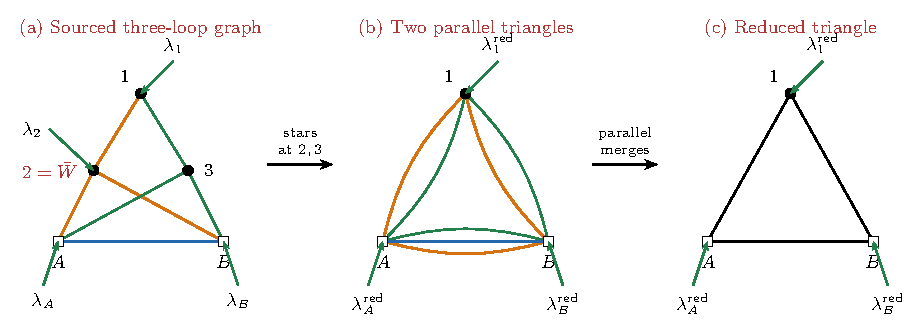
\includegraphics[width=0.96\linewidth]{figures/vec/ch6-sourced-three-loop-20261102.pdf}
\caption{The three-loop sourced example, with $2$ carrying $\bar W$ and $\lambda_2\ne0$. Removing the stars at $2$ (orange) and $3$ (green, $\lambda_3=0$) gives two triangles in parallel with the original marked edge $AB$ (blue). Parallel merging leaves the triangle on $1,A,B$ with sources $\lambda_1^{\mathrm{red}},\lambda_A^{\mathrm{red}},\lambda_B^{\mathrm{red}}$.}
\label{local-b1fa6157-692c-4e5f-b2bb-788a6f06b26a}
\end{figure}

Orient and order the edges as $(21,2A,2B,31,3A,3B,AB)$, with $\lambda_3=0$. Apply the two star--triangle changes of Theorem \ref{b-01173}, retaining the source terms \eqref{eq-1-78} at $2$, and merge the parallel sides. The reduced triangle has
\begin{equation*}
\begin{gathered}
t^{\mathrm{red}}_{1A}=1-r_5-r_6,\qquad t^{\mathrm{red}}_{1B}=r_5,\qquad t^{\mathrm{red}}_{AB}=r_6,\\
0<r_1,r_2<1,\qquad r_3,r_4>0,\quad r_3+r_4<1,\qquad r_5,r_6>0,\quad r_5+r_6<1,\\
\Sigma=\frac{1-r_5-r_6}{r_1}+\frac{r_5}{r_2}+\frac{r_6}{r_3}.
\end{gathered}
\end{equation*}
\begin{equation*}
\begin{aligned}
\lambda^{\mathrm{red}}_1&=\lambda_1+\frac{r_6/r_3}{\Sigma}\lambda_2,\\
\lambda^{\mathrm{red}}_A&=\lambda_A+\frac{r_5/r_2}{\Sigma}\lambda_2,\\
\lambda^{\mathrm{red}}_B&=\lambda_B+\frac{(1-r_5-r_6)/r_1}{\Sigma}\lambda_2,\\
y^{\mathrm{red}}_{1A}&=r_5\lambda^{\mathrm{red}}_1-r_6\lambda^{\mathrm{red}}_A,\\
y^{\mathrm{red}}_{1B}&=\lambda^{\mathrm{red}}_1-y^{\mathrm{red}}_{1A},\\
y^{\mathrm{red}}_{AB}&=\lambda^{\mathrm{red}}_A+y^{\mathrm{red}}_{1A}.
\end{aligned}
\end{equation*}
\begin{equation*}
\begin{aligned}
y_{21}&=\frac{r_6/r_3}{\Sigma}\lambda_2-r_1y^{\mathrm{red}}_{1A}-r_2y^{\mathrm{red}}_{1B},\\
y_{31}&=-(1-r_1)y^{\mathrm{red}}_{1A}-(1-r_2)y^{\mathrm{red}}_{1B},\\
y_{2A}&=\frac{r_5/r_2}{\Sigma}\lambda_2+r_1y^{\mathrm{red}}_{1A}-r_3y^{\mathrm{red}}_{AB},\\
y_{3A}&=(1-r_1)y^{\mathrm{red}}_{1A}-r_4y^{\mathrm{red}}_{AB},\\
y_{2B}&=\frac{(1-r_5-r_6)/r_1}{\Sigma}\lambda_2+r_2y^{\mathrm{red}}_{1B}+r_3y^{\mathrm{red}}_{AB},\\
y_{3B}&=(1-r_2)y^{\mathrm{red}}_{1B}+r_4y^{\mathrm{red}}_{AB},\\
y_{AB}&=(1-r_3-r_4)y^{\mathrm{red}}_{AB}.
\end{aligned}
\end{equation*}
\begin{equation*}
\begin{aligned}
z^{\mathrm{red}}_{1A}&=r_1(z_{2A}-z_{21})+(1-r_1)(z_{3A}-z_{31}),\\
z^{\mathrm{red}}_{1B}&=r_2(z_{2B}-z_{21})+(1-r_2)(z_{3B}-z_{31}),\\
z^{\mathrm{red}}_{AB}&=(1-r_3-r_4)z_{AB}+r_3(z_{2B}-z_{2A})+r_4(z_{3B}-z_{3A}),\\
\sum_{\substack{e\in I\\\mathrm{edges}}}y_{e,+\dot a}z_e^{+\dot a}
&=\lambda_{2,+\dot a}\left(\frac{r_6z_{21}/r_3+r_5z_{2A}/r_2+(1-r_5-r_6)z_{2B}/r_1}{\Sigma}\right)^{+\dot a}\\
&\quad+y^{\mathrm{red}}_{1A,+\dot a}z^{\mathrm{red},+\dot a}_{1A}
+y^{\mathrm{red}}_{1B,+\dot a}z^{\mathrm{red},+\dot a}_{1B}
+y^{\mathrm{red}}_{AB,+\dot a}z^{\mathrm{red},+\dot a}_{AB}.
\end{aligned}
\end{equation*}

Integrate over the displayed domain, at fixed original sources. The derivatives include the $r$-dependence of the transferred sources:
\begin{equation*}
\begin{aligned}
\mathcal I_\Gamma(\lambda;z)
&=\int
\bigl(-dy_{AB,+\dot+}\wedge dy_{AB,+\dot-}\bigr)
\wedge\bigl(-dy_{2B,+\dot+}\wedge dy_{2B,+\dot-}\bigr)\\
&\qquad\wedge\bigl(-dy_{3A,+\dot+}\wedge dy_{3A,+\dot-}\bigr)
\exp\!\left[-\sum_{\substack{e\in I\\\mathrm{edges}}}y_{e,+\dot a}z_e^{+\dot a}\right]\\
&=-\int\prod_{j=1}^{6}dr_j\;
\underbrace{\det\frac{\partial(y_{AB,+\dot+},y_{AB,+\dot-},y_{2B,+\dot+},y_{2B,+\dot-},y_{3A,+\dot+},y_{3A,+\dot-})}{\partial(r_1,r_2,r_3,r_4,r_5,r_6)}}_{\text{Jacobian of the three loop currents}}\\
&\qquad\times\exp\!\left[-\sum_{\substack{e\in I\\\mathrm{edges}}}y_{e,+\dot a}(r)z_e^{+\dot a}\right]\\
&=\int\prod_{j=1}^{6}dr_j\;r_5(1-r_3-r_4)(1-r_5-r_6)\,
\underbrace{\bigl(\lambda^{\mathrm{red}}_{1,+\dot a}\lambda^{\mathrm{red}}_{A,+}{}^{\dot a}\bigr)}_{\text{reduced triangle current-area factor}}\\
&\quad\times\left[\lambda^{\mathrm{red}}_{1,+\dot b}\lambda^{\mathrm{red}}_{A,+}{}^{\dot b}
+\frac{\lambda_{2,+\dot b}y^{\mathrm{red}}_{AB,+}{}^{\dot b}}{r_1r_2\Sigma}\right]\\
&\quad\times\left[(r_1-r_2)\lambda_{1,+\dot c}\lambda_{A,+}{}^{\dot c}
-\frac{(r_1-r_2)r_5(r_2-r_3)+r_2(r_2-1)}{r_2r_3\Sigma}
\lambda_{1,+\dot c}\lambda_{2,+}{}^{\dot c}\right]\\
&\quad\times\exp\!\left[-\sum_{\substack{e\in I\\\mathrm{edges}}}y_{e,+\dot d}(r)z_e^{+\dot d}\right].
\end{aligned}
\end{equation*}

Normalizing the three sides by their sum makes the source fractions in \eqref{eq-1-78} linear, but the subsequent parallel merges reintroduce denominators. In the coordinates above, take $r_2=r_3=r_4=r_5=r_6=\tfrac14$ and the source components $\lambda_{1,+\dot+}=\lambda_{2,+\dot+}=\lambda_{A,+\dot-}=1$, $\lambda_{1,+\dot-}=\lambda_{2,+\dot-}=\lambda_{A,+\dot+}=0$. Then
{\footnotesize
\begin{equation*}
\begin{aligned}
\Sigma&=\frac1{2r_1}+2,\qquad
\frac{r_6/r_3}{\Sigma}=\frac{2r_1}{1+4r_1},\\
-\left.\det\frac{\partial(y_{AB,+\dot+},y_{AB,+\dot-},y_{2B,+\dot+},y_{2B,+\dot-},y_{3A,+\dot+},y_{3A,+\dot-})}{\partial(r_1,r_2,r_3,r_4,r_5,r_6)}\right|_{\substack{r_2=\cdots=r_6=1/4\\\text{displayed sources}}}
&=\frac{(4r_1-1)(6r_1+1)(6r_1+7)}{64(4r_1+1)^2}.
\end{aligned}
\end{equation*}
}

The denominator does not cancel at zero displacement in these coordinates. The full integral is nevertheless a six-term polynomial:
\begin{equation}\label{eq-1-81}
\begin{aligned}
&\left.\mathcal I_\Gamma(\lambda;0)\right|_{\lambda_3=0}\\
&=-\int dr_1\,dr_2\,dr_3\,dr_4\,dr_5\,dr_6\;
\det\frac{\partial(y_{AB,+\dot+},y_{AB,+\dot-},y_{2B,+\dot+},y_{2B,+\dot-},y_{3A,+\dot+},y_{3A,+\dot-})}{\partial(r_1,r_2,r_3,r_4,r_5,r_6)}\\
&=\frac{\lambda_{1,+\dot a}\lambda_{2,+}{}^{\dot a}}{576}
\Bigl[
5(\lambda_{1,+\dot b}\lambda_{A,+}{}^{\dot b})^2
+12(\lambda_{1,+\dot b}\lambda_{A,+}{}^{\dot b})(\lambda_{2,+\dot c}\lambda_{A,+}{}^{\dot c})\\
&\qquad-(\lambda_{1,+\dot b}\lambda_{2,+}{}^{\dot b})(\lambda_{1,+\dot c}\lambda_{A,+}{}^{\dot c})
+3(\lambda_{2,+\dot b}\lambda_{A,+}{}^{\dot b})^2\\
&\qquad+3(\lambda_{1,+\dot b}\lambda_{2,+}{}^{\dot b})(\lambda_{2,+\dot c}\lambda_{A,+}{}^{\dot c})
-(\lambda_{1,+\dot b}\lambda_{2,+}{}^{\dot b})^2
\Bigr].
\end{aligned}
\end{equation}

To evaluate it, we combine the reductions with the quadratic identity of the graph kernels \cite[Section 3.2]{operatope}, \cite[Theorem 7]{Wang}. Keep the ordered edges $(21,2A,2B,31,3A,3B,AB)$, set $\lambda_3=0$, and extract the degree-zero displacement term (Figure~\ref{fig-B6-sourced-three-loop}).

\begin{figure}[H]
\centering
\begin{tikzpicture}
\node[anchor=south west,inner sep=0] (img) at (0,0) {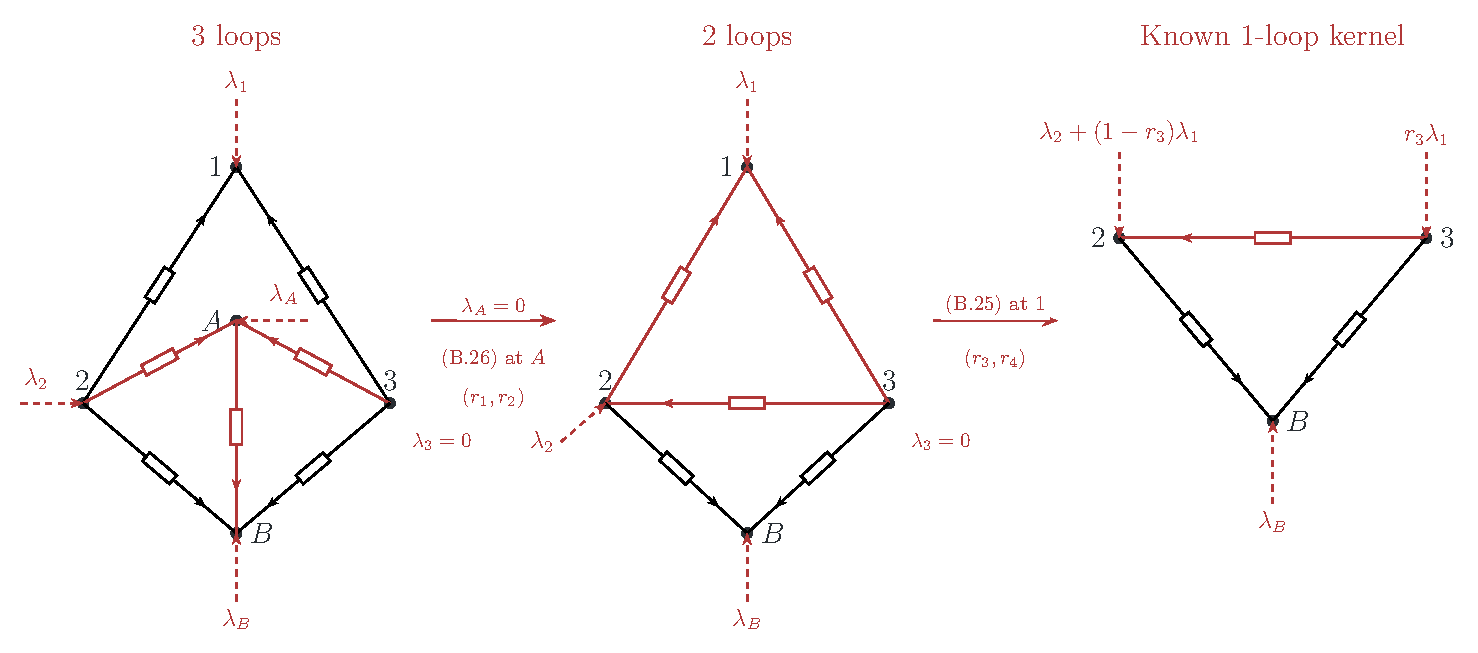
\includegraphics[width=0.96\linewidth]{figures/vec/b6-sourced-three-loop-boundary-20261108.pdf}};
\begin{scope}[x={(img.south east)},y={(img.north west)}]
\node[fill=white,inner sep=0.6pt,minimum width=0.072\linewidth,minimum height=0pt,font=\fontsize{6}{7}\selectfont,text=blue!50!black] at (0.3338,0.4490) {\eqref{eq-kernel-star-triangle} at $A$};
\node[fill=white,inner sep=0.6pt,minimum width=0.072\linewidth,minimum height=0pt,font=\fontsize{6}{7}\selectfont,text=blue!50!black] at (0.6734,0.5300) {\eqref{eq-kernel-series-parallel} at $1$};
\end{scope}
\end{tikzpicture}
\caption{The sourced three-loop graph and its boundary calculation at $\lambda_A=0$: \eqref{eq-kernel-star-triangle} at $A$, then \eqref{eq-kernel-series-parallel} at $1$, leave the known triangle kernel. The arrows retain the edge orientations and show the transferred sources.}
\label{fig-B6-sourced-three-loop}
\end{figure}

Insert a vertex $v$ on $AB$, with ordered edges $(21,2A,2B,31,3A,3B,Av,vB)$; its proper induced Laman subgraphs are the eight edges, and we choose the sources below on this six-vertex graph.
\begin{equation}\label{eq-1-79}
\begin{gathered}
0=\sum_{\substack{1\le k\le8\\e_k\,\mathrm{in}\ (21,2A,2B,31,3A,3B,Av,vB)}}
(-1)^{k-1}\,
\mathcal I_{\Gamma_{AB\mapsto Av,vB}/e_k}(\lambda;0),\\
\lambda_3=\lambda_B=0,\qquad
\lambda_v=-\lambda_1-\lambda_2-\lambda_A.
\end{gathered}
\end{equation}

Each contraction inherits the remaining edge order and adds its endpoint sources; contracting $vB$ restores the target source $\lambda_B^{\mathrm{red}}=\lambda_v=-\lambda_1-\lambda_2-\lambda_A$.

Contractions of $2A,2B,3A,3B$ are fans, evaluated by \eqref{eq-1-40}, and the other four are copies of the target graph; with the sources of \eqref{eq-1-79}, the signed fan sum is
\begin{equation*}
\begin{aligned}
&\sum_{\substack{k\in\{2,3,5,6\}\\\mathrm{fan\ contractions}}}
(-1)^{k-1}\mathcal I_{\Gamma_{AB\mapsto Av,vB}/e_k}(\lambda;0)\\
&=\frac{\lambda_{1,+\dot a}\lambda_{2,+}{}^{\dot a}
+\lambda_{1,+\dot a}\lambda_{A,+}{}^{\dot a}}{144}
\Bigl[
(\lambda_{1,+\dot b}\lambda_{2,+}{}^{\dot b})(\lambda_{1,+\dot c}\lambda_{A,+}{}^{\dot c})\\
&\qquad+2(\lambda_{1,+\dot b}\lambda_{2,+}{}^{\dot b})(\lambda_{2,+\dot c}\lambda_{A,+}{}^{\dot c})
+(\lambda_{1,+\dot b}\lambda_{A,+}{}^{\dot b})(\lambda_{2,+\dot c}\lambda_{A,+}{}^{\dot c})
+(\lambda_{2,+\dot b}\lambda_{A,+}{}^{\dot b})^2\Bigr].
\end{aligned}
\end{equation*}

\begin{proofbox}
\emph{Coefficient calculation.}

The zero-displacement kernel is a cubic polynomial in source spinor contractions; the even edge permutation $A\leftrightarrow B$ sends both remaining contractions to their negatives when $\lambda_{1,+\dot a}\lambda_{2,+}{}^{\dot a}=0$.
\begin{equation*}
\begin{gathered}
\lambda_{1,+\dot a}\lambda_{2,+}{}^{\dot a}=0
\quad\Longrightarrow\quad
\lambda_{1,+\dot a}\lambda_{B,+}{}^{\dot a}
=-\lambda_{1,+\dot a}\lambda_{A,+}{}^{\dot a},\qquad
\lambda_{2,+\dot a}\lambda_{B,+}{}^{\dot a}
=-\lambda_{2,+\dot a}\lambda_{A,+}{}^{\dot a},\\
\left.\mathcal I_\Gamma(\lambda;0)\right|_{\lambda_3=0,\,\lambda_{1,+\dot a}\lambda_{2,+}{}^{\dot a}=0}
=-\left.\mathcal I_\Gamma(\lambda;0)\right|_{\lambda_3=0,\,\lambda_{1,+\dot a}\lambda_{2,+}{}^{\dot a}=0}=0.
\end{gathered}
\end{equation*}

Thus the kernel contains the factor $\lambda_{1,+\dot a}\lambda_{2,+}{}^{\dot a}$; denote the six numerical coefficients inside the brackets of \eqref{eq-1-81}, in displayed order, by $c_0,\ldots,c_5$.

To fix the last coefficient, set $\lambda_A=0$. Apply \eqref{eq-kernel-star-triangle} with $(v,u,w,x)=(A,3,2,B)$ and coordinates $r_1,r_2$, then \eqref{eq-kernel-series-parallel} with $(v,u,w)=(1,3,2)$ and coordinates $r_3,r_4$. On the final triangle $3,2,B$, use $r_5,r_6>0$, $r_5+r_6< 1$:
\begin{equation*}
\begin{aligned}
(\lambda_3^{\mathrm{red}})^{\mathrm{red}}&=r_3\lambda_1,&
(\lambda_2^{\mathrm{red}})^{\mathrm{red}}&=\lambda_2+(1-r_3)\lambda_1,\\
(y_{32}^{\mathrm{red}})^{\mathrm{red}}
&=r_5r_3\lambda_1-r_6[\lambda_2+(1-r_3)\lambda_1],\\
\lambda_{1,+\dot a}(y_{32,+}^{\mathrm{red}})^{\mathrm{red}}{}^{\dot a}
&=-r_6\lambda_{1,+\dot a}\lambda_{2,+}{}^{\dot a},\\
(y_{3B,+\dot a}^{\mathrm{red}})^{\mathrm{red}}
(y_{2B,+}^{\mathrm{red}})^{\mathrm{red}}{}^{\dot a}
&=r_3(1-r_5-r_6)\lambda_{1,+\dot a}\lambda_{2,+}{}^{\dot a}.
\end{aligned}
\end{equation*}
\begin{equation*}
\begin{aligned}
\left.\mathcal I_\Gamma(\lambda;0)\right|_{\lambda_A=\lambda_3=0}
&=(\lambda_{1,+\dot a}\lambda_{2,+}{}^{\dot a})^3
\int_{[0,1]^4\times\{r_5,r_6>0,\ r_5+r_6<1\}}
d^6r\\
&\qquad\times\underbrace{r_1r_2r_3(1-r_5-r_6)}_{\text{\eqref{eq-kernel-star-triangle}}}
\underbrace{(-r_4r_6)}_{\text{\eqref{eq-kernel-series-parallel}}}
\underbrace{r_3}_{\text{triangle}}\\
&=(\lambda_{1,+\dot a}\lambda_{2,+}{}^{\dot a})^3
\left(\frac12\right)^3\frac13\left(\frac1{24}+\frac1{12}-\frac16\right)
=-\frac{(\lambda_{1,+\dot a}\lambda_{2,+}{}^{\dot a})^3}{576}.
\end{aligned}
\end{equation*}

Multiply \eqref{eq-1-79} by $576$ and compare, in order, the coefficients of
\begin{equation*}
\begin{gathered}
(\lambda_{1,+\dot b}\lambda_{2,+}{}^{\dot b})^2(\lambda_{1,+\dot c}\lambda_{A,+}{}^{\dot c}),\qquad
(\lambda_{1,+\dot b}\lambda_{2,+}{}^{\dot b})^2(\lambda_{2,+\dot c}\lambda_{A,+}{}^{\dot c}),\\
(\lambda_{1,+\dot b}\lambda_{2,+}{}^{\dot b})(\lambda_{1,+\dot c}\lambda_{A,+}{}^{\dot c})(\lambda_{2,+\dot d}\lambda_{A,+}{}^{\dot d}),\qquad
(\lambda_{1,+\dot b}\lambda_{2,+}{}^{\dot b})(\lambda_{2,+\dot c}\lambda_{A,+}{}^{\dot c})^2.
\end{gathered}
\end{equation*}

Dividing the third equality by $2$ gives the first four rows below; $A\leftrightarrow B$ gives the fifth, and the boundary integral gives the sixth:
\begin{equation}\label{eq-sectorintegrand}
\begin{gathered}
\begin{pmatrix}
1&0&1&0&0&0\\
1&0&0&0&1&0\\
1&-1&-1&0&0&0\\
2&-1&-1&-1&0&0\\
-2&1&2&0&0&0\\
0&0&0&0&0&1
\end{pmatrix}
\begin{pmatrix}c_0\\c_1\\c_2\\c_3\\c_4\\c_5\end{pmatrix}
=\begin{pmatrix}4\\8\\-6\\-4\\0\\-1\end{pmatrix},
\qquad \det=2,\\
(c_0,c_1,c_2,c_3,c_4,c_5)=(5,12,-1,3,3,-1).
\end{gathered}
\end{equation}

The finite system determines all six coefficients. $\square$
\end{proofbox}

The solution is \eqref{eq-1-81}.

Table~\ref{tab-product-census-general} counts these graphs through seven loops.

{\small\renewcommand{\arraystretch}{1.25}\setlength{\tabcolsep}{4pt}
\begin{xltabular}{\linewidth}{@{}lllll>{\raggedright\arraybackslash}X>{\raggedright\arraybackslash}X@{}}
\caption{Product graphs whose trees have at most one superpotential node, all other nodes cubic, up to isomorphism fixing $A,B$. Columns 3 and 6: superpotential node with at least four resistors; last column: those of column 6 reduced without a sourced star--triangle step.}\label{tab-product-census-general}\\
\toprule
$n$ & graphs & $\bar W$ node with & type~I$'$ & spiders & $\bar W$ node with $\ge4$ & reduced without a\\
\midrule\endhead
 &  & $\ge4$ resistors &  &  & resistors, not type~I$'$ & sourced star--triangle\\
3 & 11 & 3 & 8 & 8 & 0 & 0\\
4 & 46 & 23 & 23 & 19 & 10 & 4\\
5 & 200 & 135 & 59 & 37 & 92 & 29\\
6 & 874 & 680 & 152 & 71 & 557 & 144\\
7 & 3765 & 3189 & 370 & 125 & 2864 & 610\\
\bottomrule
\end{xltabular}}

\section{Quantum supercharges and $\mathcal N=4$ Yang--Mills theory}\label{sec-supercharge}

Combining the graph kernels with the BV pairing gives the quantum supercharge. For a general interaction, let $W_\Gamma$ denote the ordered Wick contractions of the fields \eqref{eq-W-fibre-explicit}, including their Koszul signs. Restoring our scalar normalization~\eqref{eq-1-7} gives
\begin{equation}\label{eq-2-3}
\begin{aligned}
Q_n\mathcal O
={}&\frac{(-1)^n}{(n+1)!\,(8\pi^2)^n}
\sum_{\substack{\Gamma\ \mathrm{labelled,\ rooted,\ Laman}}}
\Bigl[\mathcal I_\Gamma(\lambda;z)
W_\Gamma[\mathcal I^{\otimes(n+1)},\mathcal O]\Bigr],
\end{aligned}
\end{equation}

with the displacements $z$ integrated against the functional derivatives of $W_\Gamma$ as in \eqref{eq-W-jet-edge}. At $n=0$ the single-edge graph gives $Q_0\mathcal O=\{\mathcal I,\mathcal O\}_0$, which is the tree-level (classical) SUSY transformation.

The $n$-loop $Q_n$ increases the number of derivatives by $2n$ (and by more if $\mathcal I$ contains derivatives):~

Under $\lambda_{v,+\dot a}\to c\,\lambda_{v,+\dot a}$ and $z_e^{+\dot a}\to z_e^{+\dot a}/c$ at fixed $\dot a$, the displacement exponential in \eqref{eq-operatope} is invariant and the current form, with $n$ factors $dy_{e,+\dot a}$, scales as $c^n$. Since $\lambda_v$ differentiates output fields and each $z_e$-derivative takes a derivative from an input letter, $Q_n$ raises the numbers of $\partial_{+\dot+}$ and $\partial_{+\dot-}$ derivatives by $n$ each, $2n$ in total. (A similar analysis holds in all dimensions.)

An operator with $d_{\dot+}$ and $d_{\dot-}$ holomorphic derivatives can be~$Q_n$-exact (and exact under the successive differential $d_n$ of Section~\ref{sec-lifting}) only if~$n\le\min(d_{\dot+},d_{\dot-})$, so finitely many orders decide whether it becomes quantum exact.

In this section we present the main result: the loop corrections to the supercharge in $\mathcal N=4$ SYM.

In $\mathcal N=4$ SYM, all the holomorphic fields can be organized into one superfield $C$ \cite[Equation (3.52)]{BK}.

The functional derivatives we defined at displaced points are normalized by
\begin{equation}\label{eq-2-10}
\frac{\delta C^B(y,\theta')}{\delta C^A(y',\theta)}=\delta_A{}^B\,\delta^{(4)}(y-y')\prod_{I=1}^3(\theta_I-\theta'_I),
\end{equation}

\subsection{The all-order anomalous SUSY transformation}\label{the-all-order-operator}

\begin{figure}[H]
\centering
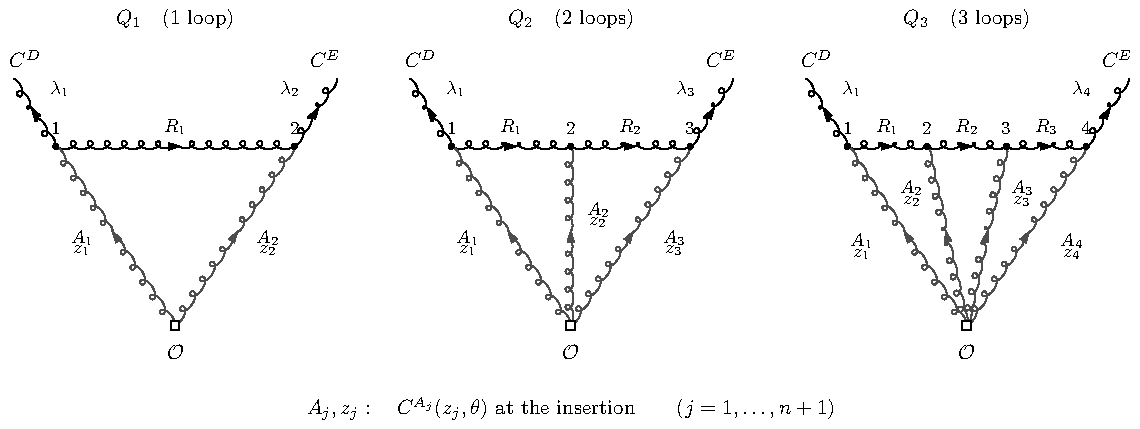
\includegraphics[width=0.96\linewidth]{figures/vec/figures-n4_three_fans.pdf}
\caption{One-, two- and three-loop supercharge fans in $\mathcal N=4$ Yang--Mills theory. The spoke labelled $A_j,z_j$ contracts an input $C^{A_j}(z_j,\theta)$ at $\mathcal O$. The path contracts the colour indices $R_1,\ldots,R_n$ and leaves the endpoint fields $C^D,C^E$, carrying $\lambda_1,\lambda_{n+1}$.}
\label{fig-n4-supercharge-fans}
\end{figure}

\rthm{Theorem}{b-00431}{} ~ \emph{For the superfield action \eqref{eq-A-15} and an operator at $x$, the $n$-loop supercharge for $n\ge1$ is}
\begin{equation}\label{eq-2-8}
\begin{aligned}
Q_n={}&\frac{(-1)^ni^{n+1}}{2(32\pi^2)^n}
\int_{\eqref{eq-1-37}}dr_1\cdots dr_{2n}\,
\left[\prod_{j=1}^{n-1}r_{2j-1}^{n-j}r_{2j}(1-r_{2j})^{j-1}\right]r_{2n}^{n-1}
\int d^3\theta\int\prod_{j=1}^{n+1}d^4z_j\\
&\times C_{A_1DR_1}
\left(\prod_{j=2}^{n}C_{A_jR_{j-1}R_j}\right)C_{A_{n+1}R_nE}\\
&\times\big(\partial_{+\dot a_1}\cdots\partial_{+\dot a_n}C^D\big)(x+x_1(r,z),\theta)
\big(\partial_+{}^{\dot a_1}\cdots\partial_+{}^{\dot a_n}C^E\big)(x+x_{n+1}(r,z),\theta)\\
&\times\frac{\delta}{\delta C^{A_1}(x+z_1,\theta)}\cdots
\frac{\delta}{\delta C^{A_{n+1}}(x+z_{n+1},\theta)},
\end{aligned}
\end{equation}
\emph{where the output fields are differentiated before they are evaluated at the translated positions.}
\begin{equation*}
\begin{aligned}
x_1^{+\dot a}(r,z)
={}&\sum_{j=1}^{n}(1-r_{2j-1})
\left(\prod_{k=1}^{j-1}r_{2k-1}\right)\\
&\times\left[
\left(\prod_{k=1}^{j-1}(1-r_{2k})\right)z_1^{+\dot a}
+\sum_{i=2}^{j}r_{2i-2}
\left(\prod_{k=i}^{j-1}(1-r_{2k})\right)z_i^{+\dot a}
\right]\\
&+\left(\prod_{k=1}^{n}r_{2k-1}\right)z_{n+1}^{+\dot a},\\[3pt]
x_{n+1}^{+\dot a}(r,z)
={}&r_{2n}\left[
\left(\prod_{k=1}^{n-1}(1-r_{2k})\right)z_1^{+\dot a}
+\sum_{i=2}^{n}r_{2i-2}
\left(\prod_{k=i}^{n-1}(1-r_{2k})\right)z_i^{+\dot a}
\right]\\
&+(1-r_{2n})z_{n+1}^{+\dot a}.
\end{aligned}
\end{equation*}

The (fan) kernel and the complete Taylor expansion in the $z_j$~are derived and listed in Section~\ref{sec-fans}.

\emph{Proof.}

The cubic term of \eqref{eq-A-15} gives the vertex $iC_{ABC}$, which includes the $3!$ assignments of its three legs, and the rooted fan has symmetry factor $1/2$ for the reversal of its interaction path.

The functional derivatives in \eqref{eq-2-8} attach the spokes to the input letters; only the two endpoint fields remain uncontracted, so $\lambda_2=\cdots=\lambda_n=0$.

In the endpoint kernel \eqref{eq-1-41}, the substitution \eqref{eq-D-lambda} gives, with $\partial_{1,+\dot a}$ and $\partial_{n+1,+\dot a}$ acting on the first and second output fields, respectively,
\begin{equation*}
\begin{aligned}
(\lambda_{1,+\dot a}\lambda_{n+1,+}{}^{\dot a})^n
\longmapsto{}&4^{-n}
\partial_{1,+\dot a_1}\cdots\partial_{1,+\dot a_n}
\partial_{n+1,+}{}^{\dot a_1}\cdots\partial_{n+1,+}{}^{\dot a_n},\\
e^{\lambda_{1,+\dot a}x_1^{+\dot a}(r,z)+
\lambda_{n+1,+\dot a}x_{n+1}^{+\dot a}(r,z)}
\longmapsto{}&
e^{-\frac12x_1^{+\dot a}(r,z)\partial_{1,+\dot a}
-\frac12x_{n+1}^{+\dot a}(r,z)\partial_{n+1,+\dot a}}.
\end{aligned}
\end{equation*}
\begin{equation*}
\begin{aligned}
&e^{-\frac12x_1^{+\dot a}(r,z)\partial_{1,+\dot a}
-\frac12x_{n+1}^{+\dot a}(r,z)\partial_{n+1,+\dot a}}
C^D(x,\theta)C^E(x,\theta)\\
&\qquad=C^D(x+x_1(r,z),\theta)C^E(x+x_{n+1}(r,z),\theta),
\qquad \frac{\partial}{\partial x^{+\dot a}}=-\frac12\partial_{+\dot a}.
\end{aligned}
\end{equation*}
\begin{equation*}
\underbrace{\frac12}_{\text{path reversal}}
\underbrace{i^{n+1}}_{\text{cubic vertices}}
\underbrace{(-8\pi^2)^{-n}}_{\text{scalar-kernel normalization}}
\underbrace{4^{-n}}_{\text{output derivatives}}
=\frac{(-1)^ni^{n+1}}{2(32\pi^2)^n}.
\end{equation*}

The path contracts the colour indices in the order $C_{A_1DR_1}(\prod_{j=2}^{n}C_{A_jR_{j-1}R_j})C_{A_{n+1}R_nE}$; inserting these factors and the density \eqref{eq-1-41} gives \eqref{eq-2-8}.\hfill\qedsymbol

In practice, the colour factor can be simplified further with the trace relations of $SU(N)$ and of the other gauge groups \cite{Repo}.

On letters without holomorphic derivatives:
\begin{equation}\label{eq-Qnzero}
\begin{aligned}
Q_n\big|_{\text{no input derivatives}}
={}&\frac{(-1)^ni^{n+1}}{2(32\pi^2)^n(n!)^3(n+1)}
\int d^3\theta\,
C_{A_1DR_1}\left(\prod_{j=2}^nC_{A_jR_{j-1}R_j}\right)
C_{A_{n+1}R_nE}\\
&\times(\partial_{+\dot a_1}\cdots\partial_{+\dot a_n}C^D)
(\partial_+{}^{\dot a_1}\cdots\partial_+{}^{\dot a_n}C^E)
\prod_{j=1}^{n+1}\frac{\delta}{\delta C^{A_j}(\theta)}.
\end{aligned}
\end{equation}

\subsection{One- and two-loop examples in $\mathcal N=4$ Yang--Mills theory}\label{examples-in-mathcal-n4-yangmills-theory}

The general-$n$ operator \eqref{eq-2-8}~can look abstract. We also display the two-loop result, a problem that has recently attracted attention \cite[Section 3.2.3]{semichiral}.
\begin{equation}\label{eq-2-17}
\begin{aligned}
Q_2={}&-\frac{i}{2(32\pi^2)^2}
\int_0^1dr_1\int_0^1dr_2\int_0^1dr_4
\int_0^{1-r_4}dr_3\,r_1r_2r_4\int d^3\theta\int\prod_{j=1}^{3}d^4z_j\\
&\times C_{A_1DR}C_{A_2RS}C_{A_3SE}\,
(\partial_{+\dot a}\partial_{+\dot b}C^D)
\big(x+x_1(r,z),\theta\big)
(\partial_+{}^{\dot a}\partial_+{}^{\dot b}C^E)
\big(x+x_3(r,z),\theta\big)\\
&\times\frac{\delta}{\delta C^{A_1}(x+z_1,\theta)}
\frac{\delta}{\delta C^{A_2}(x+z_2,\theta)}
\frac{\delta}{\delta C^{A_3}(x+z_3,\theta)},
\end{aligned}
\end{equation}
where
\begin{equation*}
\begin{aligned}
x_1^{+\dot a}(r,z)
&=(1-r_1)z_1^{+\dot a}
+r_1(1-r_3)\big[(1-r_2)z_1^{+\dot a}+r_2z_2^{+\dot a}\big]
+r_1r_3z_3^{+\dot a},\\
x_3^{+\dot a}(r,z)
&=r_4\big[(1-r_2)z_1^{+\dot a}+r_2z_2^{+\dot a}\big]
+(1-r_4)z_3^{+\dot a}.
\end{aligned}
\end{equation*}

This result extends previous results and agrees with them.

For example, the first two components below agree with \cite[Equations (3.66) and (3.67)]{BK} up to normalization:\footnote{On the physical Lagrangian subspace, with $\delta^{AB}(\gamma^I)_B\leftrightarrow\bar\phi_I{}^A$, $(\beta_I)^A\leftrightarrow-\frac{i}{\sqrt2}\psi_+^{IA}$, $\delta^{AB}\mathsf b_B\leftrightarrow\frac14f_{++}^A$, $\partial_{+\dot a}\mathsf c^A\leftrightarrow2\bar\lambda_{\dot a}^A$ and $\partial_{+\dot a}\partial_{+\dot b}\mathsf c^A\leftrightarrow2\nabla_{+(\dot a}\bar\lambda_{\dot b)}^A$, equation~\eqref{eq-2-26} becomes $Q_1(\bar\phi_1{}^A\psi_+^{1B})=\frac{i\sqrt2\,g^2}{16\pi^2}C^A{}_{RD}C^{BR}{}_E\,\bar\lambda_{\dot a}^D\bar\lambda^{E\dot a}$, the component form of the Konishi anomaly~\cite{Konishi}.}

In component form:~
\begin{equation}\label{eq-2-26}
Q_1\big(\delta^{AA'}(\gamma^1)_{A'}(\beta_1)^B\big)=\frac{g^2}{64\pi^2}C_{ARD}C_{BRE}(\partial_{+\dot a}\mathsf c^D)(\partial_+{}^{\dot a}\mathsf c^E),
\end{equation}
\begin{equation}\label{eq-2-27}
Q_1\big((\beta_1)^A(\beta_2)^B\big)=\frac{ig}{64\pi^2}(C_{ARD}C_{BRE}+C_{BRD}C_{ARE})(\partial_{+\dot a}\mathsf c^D)\,\delta^{EF}\partial_+{}^{\dot a}(\gamma^3)_F,
\end{equation}
\begin{equation}\label{eq-2-28}
Q_2\big((\beta_1)^{A_1}(\beta_2)^{A_2}(\beta_3)^{A_3}\big)=-\frac{ig^2}{48(32\pi^2)^2}\sum_{\sigma\in S_3}C_{A_{\sigma(1)}DR}C_{A_{\sigma(2)}RS}C_{A_{\sigma(3)}SE}(\partial_{+\dot a}\partial_{+\dot b}\mathsf c^D)(\partial_+{}^{\dot a}\partial_+{}^{\dot b}\mathsf c^E).
\end{equation}

\section{Multi-graviton completions and obstruction equations}\label{sec-lifting}

Quantum multiplication constructs perturbatively closed multi-graviton operators in $\mathcal N=4$ Yang--Mills theory.~ We prove their closure at arbitrary loop order (Theorem \ref{b-00630}) and, for illustration, evaluate an explicit product (Section \ref{sec-graviton-example}).\footnote{The theorem proves that multi-graviton classes stay closed; however, a closed multi-graviton can still become exact, e.g., if there is a nonclosed fortuitous class with the allowed charges. The most direct one-loop example is the lifting of a black-hole class by the Konishi correction: in the $SO(7)$ theory, the one-loop supercharge pairs a multi-graviton with a fortuitous class \cite[Section 3]{KonishiBH}, and by the theorem the multi-graviton is the exact member of the pair. Section \ref{sec-results-SOSp} and \cite[supplement, Section S3]{Repo} give the one-loop lifts in $SO(2N+1)$ and their relation to S-duality. There are many more one-loop lifts in $SO(2N+1)$ than in $SU(N)$.}

We then review the framework that uses the operators $Q_n$ to test which classical classes are lifted: the successive transfers of Section \ref{sec-homotopy-transfer} compute the perturbative obstructions of classical representatives and decide which of their closed completions are quantum coboundaries. The algorithm and the explicit results are in the supplementary material \cite{Repo}.

Since every graviton class has a closed completion, no differential maps one graviton class to another (Section \ref{sec-graviton-dr}); a lift pairs a fortuitous class with a graviton class or with another fortuitous class. This makes the quantum-correction test much lighter than a brute-force sweep. Quantum closure of a classical representative $\mathcal O_0$ means that there exist finite corrections $\mathcal O_1,\mathcal O_2,\ldots$ with $\mathbf Q(\mathcal O_0+\hbar\mathcal O_1+\hbar^2\mathcal O_2+\cdots)=0$ at every order in $\hbar$; we remind the reader that $\mathcal O_0$ itself is in general not annihilated by $\mathbf Q$ (Section \ref{sec-homotopy-transfer}). Nonperturbative corrections can also modify the cohomology.

\subsection{Perturbative closure of multi-gravitons}\label{sec-graviton-closure}

The single-graviton representatives of Chang and Yin \cite[Section 4]{ChangYin} are components of $\operatorname{Tr}(dC)^p$, where
\begin{equation}\label{b-00629}
dC=dx^{+\dot a}\frac{\partial C}{\partial x^{+\dot a}}
+d\theta_I\frac{\partial_LC}{\partial\theta_I}.
\end{equation}

\rthm{Theorem}{b-00630}{} \emph{Let $G_1,\ldots,G_m$ be single-graviton representatives. } \emph{Every iterated quantum product $\mathcal O$ of these operators, with any fixed bracketing, satisfies}
\begin{equation}\label{eq-multigraviton-closure}
\mathbf Q\mathcal O=0,\qquad
\left.\mathcal O\right|_{\hbar=0}=G_1\cdots G_m.
\end{equation}

\emph{For each fixed component, its perturbative completion has finitely many terms.}

\emph{Proof.} The classical differential acts on a single graviton by
\begin{equation}\label{eq-2-58}
Q_0(dC)=[C,dC],\qquad Q_0\operatorname{Tr}(dC)^p=\operatorname{Tr}[C,(dC)^p]=0.
\end{equation}

Let us first consider a single graviton $G$.

At order $n\ge1$, the auxiliary $\theta$ part of the $Q_n$ kernel reads:
\begin{equation}\label{eq-graviton-odd-factor}
\prod_{j=1}^{n}\prod_{I=1}^{3}
\bigl(\theta_I^{(j)}-\theta_I^{(j+1)}\bigr).
\end{equation}

A nonzero coincident value requires at least $3n$ odd derivatives. Each of the $n+1$ contracted factors of $dC$ supplies at most one, leaving degree $3n-(n+1)=2n-1>0$ in the relative odd coordinates. The kernel therefore vanishes when those coordinates coincide, so all single gravitons are $\mathbf Q$-closed at every perturbative order.
\begin{equation}\label{eq-2-60}
Q_0G=0,\qquad Q_nG=0\quad(n\geq1).
\end{equation}

Applying \eqref{eq-chain} at each binary vertex of a quantum product gives
\begin{equation}\label{b-00642}
\mathbf Q(A\star B)
=(\mathbf QA)\star B+(-1)^{|A|}A\star(\mathbf QB)=0
\qquad(\mathbf QA=\mathbf QB=0).
\end{equation}

Induction proves the first assertion. The leading term of each binary product is ordinary multiplication, giving the stated classical limit \cite[Section 5]{ChangYin}.

Finiteness follows from the \hyperref[local-ch8-finite-product-corollary]{finiteness corollary} in Section \ref{the-graph-formula}.\hfill\qedsymbol

For example, for two single gravitons $G_1$ and $G_2$, the explicit quantum product shows that $G_1G_2$ admits a quantum completion (the quantum completion is always nonunique, which is exactly the renormalization freedom), namely $G_1\star G_2$; equivalently, $G_1G_2$ is not lifted by a failure of $\mathbf Q$-closure.

\paragraph{The graviton part of the cohomology.}\label{the-graviton-part-of-the-cohomology}

At finite rank the classical cohomology consists of a graviton part, spanned by multi-graviton classes, and the remaining fortuitous classes \cite{microstates}. Theorem~\ref{b-00630} supplies every class of the graviton part with an explicit closed completion: write its classical representative as a polynomial in single-graviton representatives and replace each product by a quantum product. By Theorem \ref{b-00513}, the resulting class is independent of the bracketing and of the order of the factors. (With more auxiliary pairs one can also define quantum products of three or more factors compatible with $\mathbf Q$; they differ from the iterated products $(G_1\star G_2)\star G_3$ and $G_1\star(G_2\star G_3)$ by $\mathbf Q$-exact terms.) The same construction applies to a graviton-dressed fortuitous class $G\,\mathcal O_0$: once the fortuitous core $\mathcal O_0$ has a closed completion $\mathcal O[\mathcal O_0]$, the product $G\star\mathcal O[\mathcal O_0]$ is closed.

\subsection{An explicit example}\label{sec-graviton-example}

Take the two single-graviton representatives
\begin{equation}\label{eq-gravitoninputs}
A=\delta^{XY}(\gamma^1)_X(\gamma^1)_Y,
\qquad B=(\gamma^2)_X(\beta_1)^X,
\qquad\mathcal O_0=AB.
\end{equation}

Equation \eqref{eq-A-13}, with left differentiation, identifies both operators as components of $\operatorname{Tr}(dC)^2$:
\begin{equation}\label{local-ch8-graviton-component-expansion}
\begin{aligned}
\left.\frac{\partial_L C^A}{\partial\theta_2}\right|_{\theta_1=\theta_2=0}
&=\delta^{AX}(\gamma^2)_X-\theta_3(\beta_1)^A,\\
\left.\delta_{AB}\frac{\partial_L C^A}{\partial\theta_2}
\frac{\partial_L C^B}{\partial\theta_2}\right|_{\theta_1=\theta_2=0}
&=\delta^{XY}(\gamma^2)_X(\gamma^2)_Y-2\theta_3(\gamma^2)_X(\beta_1)^X.
\end{aligned}
\end{equation}
\begin{equation}\label{local-ch8-graviton-component-extraction}
\begin{aligned}
A&=\left.\delta_{AB}\frac{\partial_L C^A}{\partial\theta_1}
\frac{\partial_L C^B}{\partial\theta_1}\right|_{\theta=0},\\
B&=-\frac12\left.\frac{\partial_L}{\partial\theta_3}
\left(\delta_{AB}\frac{\partial_L C^A}{\partial\theta_2}
\frac{\partial_L C^B}{\partial\theta_2}\right)\right|_{\theta=0}.
\end{aligned}
\end{equation}

Gauge invariance gives $Q_0A=0$. For $B$, the superpotential term gives
\begin{equation}\label{b-00658}
Q_0B=-iC^{XYZ}(\gamma^2)_X(\gamma^2)_Y(\gamma^3)_Z=0.
\end{equation}

Both $A$ and $B$ are automatically $Q_1$-closed by Theorem \ref{b-00630}.

Using \eqref{eq-2-8}, $\mathcal O_0$ itself is not $Q_1$-closed:
\begin{equation}\label{eq-scalarfermionQ1}
Q_1\mathcal O_0
=\frac{g^2}{32\pi^2}
C^X{}_{RD}C^{YR}{}_E
(\gamma^1)_X(\gamma^2)_Y
(\partial_{+\dot a}\mathsf c^D)(\partial_+{}^{\dot a}\mathsf c^E).
\end{equation}

Without the quantum product, whether $\mathcal O_0$ is lifted needs to be examined: one has to implement an algorithm to test whether the right-hand side of \eqref{eq-scalarfermionQ1} is $Q_0$-exact. If the answer is yes, $\mathrm{RHS}=Q_0\mathcal O^{\prime}$, then $\mathcal O_0-\hbar\mathcal O^{\prime}$ is closed through one loop and the class survives at one loop (it is not $\mathbf Q$-exact since it has no derivatives); if the answer is no, $\mathcal O_0$ is lifted together with another member of the $Q_0$-cohomology.

However, with the quantum product, we can explicitly answer the question: $\mathcal O_0$ is not lifted.

Taking $\mathcal O_1=[\hbar](A\star B)$, we obtain
\begin{equation}\label{eq-2-65}
\begin{aligned}
\mathcal O_1
&=\{\mathcal I,A,B\}^{\gamma,0}\\
&={\frac{i}{8\pi^2}}
{2(ig)(-1)}
{\frac12}
{\frac14}
C_D{}^{XY}(\partial_{+\dot a}\mathsf c^D)
(\partial_+{}^{\dot a}(\gamma^1)_X)(\gamma^2)_Y\\
&=\frac{g}{32\pi^2}C_D{}^{XY}(\partial_{+\dot a}\mathsf c^D)
(\partial_+{}^{\dot a}(\gamma^1)_X)(\gamma^2)_Y.
\end{aligned}
\end{equation}

Let us verify that $Q_0\mathcal O_1+Q_1\mathcal O_0=0$.

Expanding $Q_0\mathcal O_1$ gives
\begin{equation}\label{eq-scalarfermionexpand}
\begin{aligned}
Q_0\mathcal O_1={}&\frac{g^2}{32\pi^2}C_D{}^{XY}\Bigl[
-C^D{}_{EF}(\partial_{+\dot a}\mathsf c^E)\mathsf c^F
(\partial_+{}^{\dot a}(\gamma^1)_X)(\gamma^2)_Y\\
&+C_{XE}{}^F(\partial_{+\dot a}\mathsf c^D)
(\partial_+{}^{\dot a}\mathsf c^E)(\gamma^1)_F(\gamma^2)_Y\\
&+C_{XE}{}^F(\partial_{+\dot a}\mathsf c^D)\mathsf c^E
(\partial_+{}^{\dot a}(\gamma^1)_F)(\gamma^2)_Y\\
&+C_{YE}{}^F(\partial_{+\dot a}\mathsf c^D)
(\partial_+{}^{\dot a}(\gamma^1)_X)\mathsf c^E(\gamma^2)_F
\Bigr].
\end{aligned}
\end{equation}

The first, third and fourth lines cancel by invariance of $C_{DXY}$ (the Jacobi identity):
\begin{equation}\label{b-00670}
C_{RX}{}^TC_{TYZ}+C_{RY}{}^TC_{XTZ}+C_{RZ}{}^TC_{XYT}=0.
\end{equation}

The remaining term is
\begin{equation}\label{eq-2-66}
\begin{aligned}
Q_0\mathcal O_1
&=\frac{g^2}{32\pi^2}
C_D{}^{XY}C_{XE}{}^F(\gamma^1)_F(\gamma^2)_Y
(\partial_{+\dot a}\mathsf c^D)(\partial_+{}^{\dot a}\mathsf c^E)\\
&=-\frac{g^2}{32\pi^2}
C^X{}_{RD}C^{YR}{}_{E}(\gamma^1)_X(\gamma^2)_Y
(\partial_{+\dot a}\mathsf c^D)(\partial_+{}^{\dot a}\mathsf c^E)\\
&=-Q_1\mathcal O_0.
\end{aligned}
\end{equation}

The one-loop term of the quantum product therefore cancels the variation of the ordinary product of the two gravitons. The component degrees $\deg_\theta\mathcal O_0=5$ and $\deg_\theta\mathcal O_1=2$ make the quantum product terminate after its one-loop term:
\begin{equation}\label{eq-finiteexample}
\begin{gathered}
\mathcal O=A\star B=\mathcal O_0+\hbar\mathcal O_1,\qquad
Q_{n\ge2}\mathcal O_0=Q_{n\ge1}\mathcal O_1=0,\\
\mathbf Q\mathcal O
=\hbar(Q_1\mathcal O_0+Q_0\mathcal O_1)=0.
\end{gathered}
\end{equation}

The displayed one-loop completion is the full perturbative product.

For other, more complicated classes, the two-loop term $Q_2\mathcal O_0$ might not vanish automatically, but the quantum product provides the completion at every order.

\subsection{Homotopy transfer and successive obstructions}\label{sec-homotopy-transfer}

Having derived the full $Q_2$ and $Q_n$ results, we now review the foundations of homotopy transfer.
\begin{equation}\label{eq-liftingequations}
\mathbf Q\bigl(\mathcal O_0+\hbar\mathcal O_1+\hbar^2\mathcal O_2+\cdots\bigr)=0
\quad\Longleftrightarrow\quad
\sum_{\substack{j=0\\\text{loop orders}}}^{s}Q_j\mathcal O_{s-j}=0
\qquad(s\ge0).
\end{equation}

\paragraph{Successive contractions.}\label{successive-contractions}

Let $E_0$ be the complex of holomorphic local operators and set $d_0=Q_0$. The pages are iterated cohomologies,
\begin{equation}\label{eq-page-iterated}
\begin{gathered}
E_1=H(Q_0),\qquad
E_2=H\bigl(H(Q_0),d_1\bigr),\qquad
E_3=H\bigl(H(H(Q_0),d_1),d_2\bigr),\\
\ldots,\qquad
E_{r+1}=H(E_r,d_r),
\end{gathered}
\end{equation}

The first differential is $d_1[\mathcal O_0]_1=[Q_1\mathcal O_0]_1$, and $Q_1^2=-(Q_0Q_2+Q_2Q_0)$ gives $d_1^2=0$ on $H(Q_0)$. For $r\ge2$, the page obstruction includes the corrections to the representative:
\begin{equation}\label{local-ch8-obstruction-definition}
d_r[\mathcal O_0]_r=
\left[\sum_{\substack{j=1\\\text{loop orders}}}^{r}Q_j\mathcal O_{r-j}\right]_r,
\qquad
\sum_{\substack{j=0\\\text{loop orders}}}^{s}Q_j\mathcal O_{s-j}=0\quad(0\le s<r).
\end{equation}

Successive transfer constructs these maps from $\mathbf Q$; the calculation below gives $d_r^2=0$ on $E_r$. Choose an inclusion $i_r:E_{r+1}\to E_r$ of cohomology representatives, a projection $\pi_r:E_r\to E_{r+1}$, and a homotopy $h_r:E_r\to E_r$ of degree $-1$, satisfying
\begin{equation}\label{eq-page-contraction}
\begin{gathered}
\pi_ri_r=1,\qquad d_ri_r=\pi_rd_r=0,\qquad
d_rh_r+h_rd_r=1-i_r\pi_r,\\
h_ri_r=\pi_rh_r=h_r^2=0.
\end{gathered}
\end{equation}

For a $d_r$-closed representative $a\in E_r$, the contraction separates its chosen cohomology representative from its exact part:
\begin{equation}\label{local-ch8-representative-decomposition}
d_ra=0
\quad\Longrightarrow\quad
a=i_r\pi_ra+\underbrace{d_rh_ra}_{\text{exact part}},
\qquad
Q_0\mathcal O_0=0
\quad\Longrightarrow\quad
\mathcal O_0=i_0\pi_0\mathcal O_0+Q_0h_0\mathcal O_0.
\end{equation}

Write $\mathbf Q^{(0)}=\mathbf Q$. The superscript $(r)$ counts transfers, while $Q_n$ is the original $n$-loop coefficient; $[\hbar^j]$ extracts the coefficient of $\hbar^j$.
\begin{equation}\label{local-f6c8e4e4-0aee-4848-9206-eb392052b047}
\begin{gathered}
\mathbf Q^{(0)}=Q_0+\hbar Q_1+\hbar^2Q_2+\cdots,\\
\mathbf Q^{(r)}=d_r+\hbar\bigl([\hbar]\mathbf Q^{(r)}\bigr)
+\hbar^2\bigl([\hbar^2]\mathbf Q^{(r)}\bigr)+\cdots,
\qquad d_r=[\hbar^0]\mathbf Q^{(r)},\\
Q_n:E_0^k\to E_0^{k+1},\qquad
\mathbf Q^{(r)}:E_r^k[[\hbar]]\to E_r^{k+1}[[\hbar]],\qquad
d_r:E_r^k\to E_r^{k+1}.
\end{gathered}
\end{equation}

Here $k$ is the cohomological degree and $E_r[[\hbar]]$ consists of formal series with coefficients in $E_r$; the coefficient $[\hbar^0]$ is the part independent of $\hbar$.

The transferred differential and corrected maps are
\begin{equation}\label{eq-page-transfer}
\begin{aligned}
i_r(\hbar)
&=\bigl[1+h_r(\mathbf Q^{(r)}-d_r)\bigr]^{-1}i_r,\\
\pi_r(\hbar)
&=\pi_r\bigl[1+(\mathbf Q^{(r)}-d_r)h_r\bigr]^{-1},\\
h_r(\hbar)
&=\bigl[1+h_r(\mathbf Q^{(r)}-d_r)\bigr]^{-1}h_r,\\
\mathbf Q^{(r+1)}
&=\frac1\hbar\pi_r(\mathbf Q^{(r)}-d_r)i_r(\hbar),
&d_{r+1}&=\left.\mathbf Q^{(r+1)}\right|_{\hbar=0}.
\end{aligned}
\end{equation}
\begin{equation}\label{local-e52b9a7e-2ebd-454e-bac8-73e190f43160}
\begin{gathered}
E_{r+1}^k=\frac{\ker(d_r:E_r^k\to E_r^{k+1})}
{\operatorname{im}(d_r:E_r^{k-1}\to E_r^k)},\\
E_1\xrightarrow{\ i_0\ }E_0\xrightarrow{\ Q_1\ }E_0\xrightarrow{\ \pi_0\ }E_1,
\qquad d_1=\pi_0Q_1i_0,\\
i_r(\hbar)=i_r-\hbar h_r\bigl([\hbar]\mathbf Q^{(r)}\bigr)i_r+\cdots.
\end{gathered}
\end{equation}
\begin{equation}\label{eq-page-transfer-identities}
\begin{aligned}
\mathbf Q^{(r)}i_r(\hbar)
&=\hbar i_r(\hbar)\mathbf Q^{(r+1)},\\
\pi_r(\hbar)\mathbf Q^{(r)}
&=\hbar\mathbf Q^{(r+1)}\pi_r(\hbar),\\
\mathbf Q^{(r)}h_r(\hbar)+h_r(\hbar)\mathbf Q^{(r)}
&=1-i_r(\hbar)\pi_r(\hbar),\\
\pi_r(\hbar)i_r(\hbar)&=1,
&\bigl(\mathbf Q^{(r+1)}\bigr)^2&=0.
\end{aligned}
\end{equation}

Starting from $\mathbf Q^2=0$, these identities prove nilpotence successively:
\begin{equation}\label{local-e7bff0bc-9d66-44d3-8aee-afde4475cf2f}
\begin{aligned}
0&=(\mathbf Q^{(r)})^2i_r(\hbar)
=\hbar^2i_r(\hbar)(\mathbf Q^{(r+1)})^2,\\
0&=\hbar^2\pi_r(\hbar)i_r(\hbar)(\mathbf Q^{(r+1)})^2
=\hbar^2(\mathbf Q^{(r+1)})^2,\\
(\mathbf Q^{(r+1)})^2&=0,
\qquad d_{r+1}^2=[\hbar^0](\mathbf Q^{(r+1)})^2=0,\\
\operatorname{im}d_{r+1}&\subseteq\ker d_{r+1}.
\end{aligned}
\end{equation}

The third line follows by equating coefficients of formal series.

The first four obstruction maps make the successive transfers explicit.

\paragraph{The first obstruction maps.}\label{the-first-obstruction-maps}

Writing $[\hbar^k]$ for the coefficient of $\hbar^k$, the first transfer has coefficients
\begin{equation}\label{eq-first-page-series}
\begin{aligned}
[\hbar^0]\mathbf Q^{(1)}&=\pi_0Q_1i_0,\\
[\hbar]\mathbf Q^{(1)}&=\pi_0(Q_2-Q_1h_0Q_1)i_0,\\
[\hbar^2]\mathbf Q^{(1)}&=\pi_0\bigl(
Q_3-Q_2h_0Q_1-Q_1h_0Q_2
+Q_1h_0Q_1h_0Q_1\bigr)i_0.
\end{aligned}
\end{equation}

The maps $\pi_0,i_0,h_0$ form the original contraction of the full physical operator complex onto its classical $Q_0$-cohomology.

In particular,
\begin{equation}\label{eq-page-differentials}
\begin{gathered}
d_{r+1}=\pi_r\bigl([\hbar]\mathbf Q^{(r)}\bigr)i_r,\\
\begin{aligned}
d_1&=\pi_0\bigl([\hbar]\mathbf Q^{(0)}\bigr)i_0,\\
d_2&=\pi_1\bigl([\hbar]\mathbf Q^{(1)}\bigr)i_1,\\
d_3&=\pi_2\bigl([\hbar]\mathbf Q^{(2)}\bigr)i_2,\\
d_4&=\pi_3\bigl([\hbar]\mathbf Q^{(3)}\bigr)i_3.
\end{aligned}
\end{gathered}
\end{equation}
\begin{equation}\label{b-00699}
\begin{aligned}
d_1&=\pi_0Q_1i_0,\\
d_2&=\pi_1\pi_0(Q_2-Q_1h_0Q_1)i_0i_1,\\
d_3&=\pi_2\pi_1\Bigl([\hbar^2]\mathbf Q^{(1)}-
\bigl([\hbar]\mathbf Q^{(1)}\bigr)h_1\bigl([\hbar]\mathbf Q^{(1)}\bigr)\Bigr)i_1i_2,\\
d_4&=\pi_3\pi_2\Bigl([\hbar^2]\mathbf Q^{(2)}-
\bigl([\hbar]\mathbf Q^{(2)}\bigr)h_2\bigl([\hbar]\mathbf Q^{(2)}\bigr)\Bigr)i_2i_3.
\end{aligned}
\end{equation}

The coefficients on each page are obtained from the same expansion:
\begin{equation}\label{local-ch8-transfer-coefficients}
\begin{aligned}
[\hbar]\mathbf Q^{(r+1)}
&=\pi_r\Bigl([\hbar^2]\mathbf Q^{(r)}-
\bigl([\hbar]\mathbf Q^{(r)}\bigr)h_r\bigl([\hbar]\mathbf Q^{(r)}\bigr)\Bigr)i_r,\\
[\hbar^2]\mathbf Q^{(r+1)}
&=\pi_r\Bigl([\hbar^3]\mathbf Q^{(r)}
-\bigl([\hbar^2]\mathbf Q^{(r)}\bigr)h_r\bigl([\hbar]\mathbf Q^{(r)}\bigr)\\
&\qquad-\bigl([\hbar]\mathbf Q^{(r)}\bigr)h_r\bigl([\hbar^2]\mathbf Q^{(r)}\bigr)
+\bigl([\hbar]\mathbf Q^{(r)}\bigr)h_r\bigl([\hbar]\mathbf Q^{(r)}\bigr)h_r\bigl([\hbar]\mathbf Q^{(r)}\bigr)\Bigr)i_r.
\end{aligned}
\end{equation}
\begin{equation}\label{local-ch8-first-page-four-loop}
\begin{aligned}
[\hbar^3]\mathbf Q^{(1)}=\pi_0\Bigl(
&Q_4-Q_3h_0Q_1-Q_2h_0Q_2-Q_1h_0Q_3\\
&+Q_2h_0Q_1h_0Q_1+Q_1h_0Q_2h_0Q_1+Q_1h_0Q_1h_0Q_2\\
&-Q_1h_0Q_1h_0Q_1h_0Q_1\Bigr)i_0.
\end{aligned}
\end{equation}

The second term in $d_2$ is the contribution of the first correction to the representative.

To see this directly, take $\mathcal O_0=i_0i_1a$ with $a\in E_2$, and choose $\mathcal O_1=-h_0Q_1\mathcal O_0$.~ Then
\begin{equation}\label{eq-d2closure}
\begin{aligned}
Q_0\mathcal O_1
&=-(1-i_0\pi_0)Q_1\mathcal O_0=-Q_1\mathcal O_0,\\
Q_0(Q_2\mathcal O_0+Q_1\mathcal O_1)
&=-Q_1^2\mathcal O_0-Q_1Q_0\mathcal O_1=0,\\
\pi_1\pi_0(Q_2\mathcal O_0+Q_1\mathcal O_1)&=d_2a.
\end{aligned}
\end{equation}

Equivalently, with $[\cdot]_r$ denoting a class in $E_r$,
\begin{equation}\label{eq-d2}
d_2[\mathcal O_0]_2
=[Q_2\mathcal O_0+Q_1\mathcal O_1]_2.
\end{equation}

Changing $\mathcal O_1$ by a classical cocycle changes the projected obstruction by a $d_1$-boundary, so it does not affect the $d_2$ obstruction equation.

\paragraph{Corrected representatives.}\label{corrected-representatives}

For a class $a\in E_3$, the condition $d_2i_2a=0$ gives the following choice of corrections through two loops:
\begin{equation}\label{eq-two-loop-representative-transfer}
\begin{aligned}
\mathcal O_0&=i_0i_1i_2a,\\
\mathcal O_1
&=-h_0Q_1\mathcal O_0
-i_0h_1\pi_0(Q_2-Q_1h_0Q_1)\mathcal O_0,\\
\mathcal O_2&=-h_0(Q_2\mathcal O_0+Q_1\mathcal O_1).
\end{aligned}
\end{equation}
\begin{equation}\label{b-00707}
\begin{gathered}
\{\mathcal O_1:Q_0\mathcal O_1=-Q_1\mathcal O_0\}
=-h_0Q_1\mathcal O_0+\ker Q_0,\\
Q_0\mathcal O_2=-(Q_2\mathcal O_0+Q_1\mathcal O_1),
\qquad \pi_0(Q_2\mathcal O_0+Q_1\mathcal O_1)=0,\\
Q_0\Bigl[-i_0h_1\pi_0(Q_2-Q_1h_0Q_1)\mathcal O_0\Bigr]=0.
\end{gathered}
\end{equation}

The second-order equation selects a $Q_0$-closed addition to the first-order solution:
\begin{equation}\label{eq-two-loop-representative-projection}
\begin{aligned}
\pi_0(Q_2\mathcal O_0+Q_1\mathcal O_1)
&=(1-d_1h_1)\pi_0(Q_2-Q_1h_0Q_1)\mathcal O_0\\
&=i_1\pi_1\pi_0(Q_2-Q_1h_0Q_1)\mathcal O_0\\
&=i_1d_2i_2a=0,\qquad a\in E_3.
\end{aligned}
\end{equation}

The choice of $\mathcal O_2$ above solves the second-order equation; a further $Q_0$-closed term gives another such choice.

For a homogeneous component in $\mathcal N=4$ theory, the grading of Appendix \ref{sec-E-sectors} gives
\begin{equation}\label{local-ch8-finite-correction-degree}
\begin{gathered}
\deg_\theta\mathcal O_s=\deg_\theta\mathcal O_0-3s,
\qquad \mathcal O_s=0\quad\text{if }3s>\deg_\theta\mathcal O_0,\\
\deg_\theta(d_r[\mathcal O_0]_r)=\deg_\theta\mathcal O_0-3r
\quad\text{whenever }d_r[\mathcal O_0]_r\ne0.
\end{gathered}
\end{equation}

On every page the same construction gives
\begin{equation}\label{eq-page-representative-chain}
\mathbf Q\,i_0(\hbar)\cdots i_{r-1}(\hbar)
=\hbar^r i_0(\hbar)\cdots i_{r-1}(\hbar)\mathbf Q^{(r)}.
\end{equation}

For $a\in E_{r+1}$, choose $\mathcal O_s$ as the coefficient of $\hbar^s$ in $i_0(\hbar)\cdots i_{r-1}(\hbar)i_ra$. Then
\begin{equation}\label{eq-2-75}
\sum_{\substack{k=0\\\text{loop orders}}}^{s}Q_k\mathcal O_{s-k}=0\quad(0\le s\le r),
\qquad
d_{r+1}[\mathcal O_0]_{r+1}
=\left[\sum_{\substack{k=1\\\text{loop orders}}}^{r+1}Q_k\mathcal O_{r+1-k}\right]_{r+1}.
\end{equation}

For $a\in E_4$, expand $i_0(\hbar)i_1(\hbar)i_2(\hbar)i_3a$ to first order:
\begin{equation}\label{local-5a4a4408-fb00-44ca-9386-984ed2933cca}
\begin{aligned}
[\hbar]i_r(\hbar)&=-h_r\bigl([\hbar]\mathbf Q^{(r)}\bigr)i_r,\\
\mathcal O_0&=i_0i_1i_2i_3a,\\
\mathcal O_1&=-h_0Q_1\mathcal O_0
-i_0h_1\bigl([\hbar]\mathbf Q^{(1)}\bigr)i_1i_2i_3a\\
&\quad-i_0i_1h_2\bigl([\hbar]\mathbf Q^{(2)}\bigr)i_2i_3a.
\end{aligned}
\end{equation}
\begin{equation}\label{local-ch8-lower-page-cocycle-check}
\begin{gathered}
Q_0i_0i_1h_2=0,\qquad d_1\pi_0i_0i_1h_2=d_1i_1h_2=0,\\
\pi_2\bigl([\hbar]\mathbf Q^{(2)}\bigr)i_2i_3a=d_3i_3a=0,\\
d_2\Bigl[-h_2\bigl([\hbar]\mathbf Q^{(2)}\bigr)i_2i_3a\Bigr]
=-\bigl([\hbar]\mathbf Q^{(2)}\bigr)i_2i_3a.
\end{gathered}
\end{equation}

The last term in $\mathcal O_1$ preserves the preceding closure equations and supplies the next compatibility condition.

\paragraph{Products and classical representatives.}\label{products-and-classical-representatives}

Suppose the operators $A=\sum_{s<r}\hbar^sA_s$ and $B=\sum_{s<r}\hbar^sB_s$~already satisfy the closure equations through order $r-1$. Write $\mathcal O_s=[\hbar^s](A\star B)$. The leading term is $\mathcal O_0=A_0B_0$. Taking coefficients in \eqref{eq-chain} gives
\begin{equation}\label{eq-2-77}
\begin{gathered}
\sum_{\substack{k=0\\\text{loop orders}}}^{s}Q_k\mathcal O_{s-k}=0\qquad(0\le s<r),\\
\begin{aligned}
Q_0\mathcal O_r+\sum_{\substack{k=1\\\text{loop orders}}}^{r}Q_k\mathcal O_{r-k}
={}&\Bigl(\sum_{\substack{k=1\\\text{loop orders}}}^{r}Q_kA_{r-k}\Bigr)B_0\\
&+(-1)^{|A_0|}A_0\Bigl(\sum_{\substack{k=1\\\text{loop orders}}}^{r}Q_kB_{r-k}\Bigr).
\end{aligned}
\end{gathered}
\end{equation}

Passing to $E_r$ gives
\begin{equation}\label{eq-2-78}
\begin{aligned}
[A_0]_r[B_0]_r&=[A_0B_0]_r,\\
d_r([A_0]_r[B_0]_r)
&=(d_r[A_0]_r)[B_0]_r
+(-1)^{|A_0|}[A_0]_r(d_r[B_0]_r).
\end{aligned}
\end{equation}

Starting from multiplication on $H(Q_0)$, this identity gives an associative graded-commutative product on each successive page.
\begin{equation}\label{sentence-83f2db8a75f1b6ffe6de850c}
E_{r+1}^k=\frac{\ker d_r^k}{\operatorname{im}d_r^{k-1}},
\qquad d_r^k:E_r^k\to E_r^{k+1}.
\end{equation}
\begin{equation}\label{local-882cf329-2e67-4239-8e6d-1d9c611ce149}
\begin{gathered}
d_r[A_0]_r=d_r[B_0]_r=0\quad\Longrightarrow\quad d_r[A_0B_0]_r=0,\\
[A_0]_r=d_ra,\quad d_r[B_0]_r=0
\quad\Longrightarrow\quad
[A_0B_0]_r=d_r\bigl(a[B_0]_r\bigr),\\
[A_0]_{r+1}[B_0]_{r+1}=[A_0B_0]_{r+1},\\
[A_0]_{r+1}[B_0]_{r+1}=0
\quad\Longleftrightarrow\quad
[A_0B_0]_r\in\operatorname{im}d_r.
\end{gathered}
\end{equation}

\paragraph{Higher differentials on the graviton part.}\label{sec-graviton-dr}

Applying the projection identity in \eqref{eq-page-transfer-identities} on successive pages gives
\begin{equation}\label{eq-graviton-dr}
\pi_{r-1}(\hbar)\cdots\pi_0(\hbar)\,\mathbf Q
=\hbar^r\,\mathbf Q^{(r)}\,\pi_{r-1}(\hbar)\cdots\pi_0(\hbar).
\end{equation}

If $\mathbf Q\mathcal O=0$, dividing \eqref{eq-graviton-dr} applied to $\mathcal O$ by $\hbar^r$ gives $\mathbf Q^{(r)}\pi_{r-1}(\hbar)\cdots\pi_0(\hbar)\mathcal O=0$. Its constant term is $d_r\pi_{r-1}\cdots\pi_0\mathcal O_0$, and by induction on $r$ the projection $\pi_{r-1}\cdots\pi_0\mathcal O_0$ is the class $[\mathcal O_0]_r$. Hence, a class with a closed completion satisfies
\begin{equation}\label{eq-graviton-dr-zero}
d_r[\mathcal O_0]_r=0\qquad(r\ge1).
\end{equation}

By Theorem~\ref{b-00630}, every $d_r$ with $r\ge1$ vanishes on the graviton part. For $d_r^k:E_r^k\to E_r^{k+1}$, the dimensions satisfy
\begin{equation}\label{local-ch8-page-rank-identity}
\begin{aligned}
\operatorname{rank}d_r^k&=\dim E_r^k-\dim\ker d_r^k,\\
\dim E_{r+1}^k&=\dim E_r^k-\operatorname{rank}d_r^k-\operatorname{rank}d_r^{k-1}.
\end{aligned}
\end{equation}
\begin{equation}\label{local-ff66fcbd-a688-489d-b2a5-4566eb361cd3}
\begin{aligned}
\operatorname{rank}d_r^k
={}&\dim\left\{[\mathcal O_0]_1\in E_1^k:
\begin{array}{l}
\exists\,\mathcal O_1,\ldots,\mathcal O_{r-1},\\
\displaystyle\sum_{\substack{j=0\\\text{loop orders}}}^{s}Q_j\mathcal O_{s-j}=0\quad(0\le s<r)
\end{array}\right\}\\
&-\dim\left\{[\mathcal O_0]_1\in E_1^k:
\begin{array}{l}
\exists\,\mathcal O_1,\ldots,\mathcal O_r,\\
\displaystyle\sum_{\substack{j=0\\\text{loop orders}}}^{s}Q_j\mathcal O_{s-j}=0\quad(0\le s\le r)
\end{array}\right\}.
\end{aligned}
\end{equation}
\begin{equation}\label{sentence-2a40039ce98c2864b4c2c6f7}
d_r[\mathcal O_0]_r=0\quad(\mathcal O_0\text{ a multi-graviton}),
\qquad
[\mathcal O_0]_{r+1}=0
\quad\Longleftrightarrow\quad
[\mathcal O_0]_r\in\operatorname{im}d_r^{k-1}.
\end{equation}

The extension spaces are nested and contain the graviton part, so for any finite number $R$ of pages,
\begin{equation}\label{local-ch8-fortuitous-rank-bound}
\sum_{\substack{r=1\\\text{pages}}}^{R}\operatorname{rank}d_r^k
\le\dim E_1^k-
\dim\operatorname{span}\left\{[\mathcal O_0]_1\in E_1^k:\mathcal O_0\text{ is a multi-graviton}\right\}.
\end{equation}

Fortuitous classes are sparse among the classical classes known so far \cite{microstates,KKLP}, so the successive differentials are extremely sparse on the known cohomology.

For completed operators satisfying
\begin{equation}\label{eq-incoming-exactness}
\mathbf Q X=\hbar^r\mathcal O,\qquad
\mathbf Q\mathcal O=0,
\qquad
\mathcal O=\mathbf Q(\hbar^{-r}X),
\end{equation}
the last equality holds after inverting $\hbar$. Over formal power series, the first equality records a class annihilated by $\hbar^r$. The successive pages record these $d_r$-exact classes at their respective orders in $\hbar$.
\begin{equation}\label{local-ch8-incoming-page-boundary}
\mathbf QX=\hbar^r\mathcal O
\quad\Longrightarrow\quad
d_r[X_0]_r=[\mathcal O_0]_r,
\qquad [\mathcal O_0]_{r+1}=0,
\qquad X_0=[\hbar^0]X.
\end{equation}

\rthm{Proposition}{prop-ch8-transfer-validity}{Validity of successive homotopy transfer}

Let $\mathbf Q^{(r)}$ be a formal differential on $E_r[[\hbar]]$, with $(\mathbf Q^{(r)})^2=0$ and constant coefficient $d_r$, and choose a contraction as in \eqref{eq-page-contraction}.

The maps defined by \eqref{eq-page-transfer} are well defined coefficientwise and satisfy all identities in \eqref{eq-page-transfer-identities}; consequently the successive transfers and the representative chain \eqref{eq-page-representative-chain} hold.

For the homogeneous $\mathcal N=4$ contractions of \eqref{local-ch8-transfer-grading}, both inverse series terminate on every fixed homogeneous polynomial input.

\begin{proofbox}
\emph{Proof.}

The starting contraction can be chosen degree by degree: select representatives of $\ker d_r/\operatorname{im}d_r$ and a complement of $\ker d_r$ in $E_r$.

Take $i_r$ to be the representative inclusion, $\pi_r$ the projection onto these representatives followed by their cohomology classes, and $h_r$ the inverse of $d_r$ from its image to the chosen complement, extended by zero on the representatives and the complement.

On the representatives, boundaries and complement, $d_rh_r+h_rd_r$ acts respectively as $0,1,1$, while $1-i_r\pi_r$ has the same action; the remaining identities in \eqref{eq-page-contraction} follow from these definitions.

Since $\mathbf Q^{(r)}-d_r$ has zero constant coefficient, the inverses are the following formal series, with $k$ counting powers of the displayed operator:
\begin{equation}\label{eq-ch8-transfer-inverses}
\begin{aligned}
\bigl[1+h_r(\mathbf Q^{(r)}-d_r)\bigr]^{-1}
&=\sum_{\substack{k\ge0\\\text{operator powers}}}
(-1)^k\bigl[h_r(\mathbf Q^{(r)}-d_r)\bigr]^k,\\
\bigl[1+(\mathbf Q^{(r)}-d_r)h_r\bigr]^{-1}
&=\sum_{\substack{k\ge0\\\text{operator powers}}}
(-1)^k\bigl[(\mathbf Q^{(r)}-d_r)h_r\bigr]^k.
\end{aligned}
\end{equation}

At coefficient order $\hbar^n$, terms with $k>n$ vanish, so each coefficient is a finite sum; multiplying the series by its denominator cancels adjacent powers and gives the identity.
\begin{equation}\label{eq-ch8-transfer-resolvent-identities}
\begin{aligned}
i_r(\hbar)&=i_r-h_r(\hbar)(\mathbf Q^{(r)}-d_r)i_r,\\
\pi_r(\hbar)&=\pi_r-\pi_r(\mathbf Q^{(r)}-d_r)h_r(\hbar),\\
h_r(\hbar)&=\bigl[1+h_r(\mathbf Q^{(r)}-d_r)\bigr]^{-1}h_r\\
&=h_r\bigl[1+(\mathbf Q^{(r)}-d_r)h_r\bigr]^{-1}.
\end{aligned}
\end{equation}

The last equality follows term by term from associativity of composition; using $h_r^2=h_ri_r=\pi_rh_r=0$ gives
\begin{equation}\label{eq-ch8-transfer-side-conditions}
\begin{gathered}
h_r\bigl[1+h_r(\mathbf Q^{(r)}-d_r)\bigr]^{-1}=h_r,\\
h_r(\hbar)^2
=\bigl[1+h_r(\mathbf Q^{(r)}-d_r)\bigr]^{-1}h_r^2=0,\\
h_r(\hbar)i_r=0,\qquad \pi_rh_r(\hbar)=0.
\end{gathered}
\end{equation}
\begin{equation}\label{eq-ch8-transfer-retraction-proof}
\begin{aligned}
\pi_r(\hbar)i_r(\hbar)
={}&\pi_ri_r-\pi_rh_r(\hbar)(\mathbf Q^{(r)}-d_r)i_r\\
&-\pi_r(\mathbf Q^{(r)}-d_r)h_r(\hbar)i_r\\
&+\pi_r(\mathbf Q^{(r)}-d_r)h_r(\hbar)^2(\mathbf Q^{(r)}-d_r)i_r=1,\\
h_r(\hbar)i_r(\hbar)&=0,\qquad
\pi_r(\hbar)h_r(\hbar)=0.
\end{aligned}
\end{equation}

From $(\mathbf Q^{(r)})^2=d_r^2=0$,
\begin{equation}\label{eq-ch8-transfer-perturbation-algebra}
\begin{aligned}
&(\mathbf Q^{(r)}-d_r)\mathbf Q^{(r)}
+\mathbf Q^{(r)}(\mathbf Q^{(r)}-d_r)\\
&=-d_r\mathbf Q^{(r)}-\mathbf Q^{(r)}d_r
=(\mathbf Q^{(r)}-d_r)^2.
\end{aligned}
\end{equation}

Multiplication by the two inverse denominators gives the explicit homotopy calculation:
\begin{equation}\label{eq-ch8-transfer-homotopy-calculation}
\begin{aligned}
&\bigl[1+h_r(\mathbf Q^{(r)}-d_r)\bigr]
\bigl(\mathbf Q^{(r)}h_r(\hbar)+h_r(\hbar)\mathbf Q^{(r)}\bigr)\\
&\qquad\times\bigl[1+(\mathbf Q^{(r)}-d_r)h_r\bigr]\\
&=\mathbf Q^{(r)}h_r+h_r\mathbf Q^{(r)}\\
&\quad+h_r\bigl[(\mathbf Q^{(r)}-d_r)\mathbf Q^{(r)}
+\mathbf Q^{(r)}(\mathbf Q^{(r)}-d_r)\bigr]h_r\\
&=1-i_r\pi_r+(\mathbf Q^{(r)}-d_r)h_r
+h_r(\mathbf Q^{(r)}-d_r)\\
&\quad+h_r(\mathbf Q^{(r)}-d_r)^2h_r\\
&=\bigl[1+h_r(\mathbf Q^{(r)}-d_r)\bigr]
\bigl[1+(\mathbf Q^{(r)}-d_r)h_r\bigr]-i_r\pi_r.
\end{aligned}
\end{equation}

Applying the inverses already established yields
\begin{equation}\label{eq-ch8-transfer-homotopy-proved}
\mathbf Q^{(r)}h_r(\hbar)+h_r(\hbar)\mathbf Q^{(r)}
=1-i_r(\hbar)\pi_r(\hbar).
\end{equation}
\begin{equation}\label{eq-ch8-transfer-invariance}
\begin{aligned}
\mathbf Q^{(r)}i_r(\hbar)\pi_r(\hbar)
&=\mathbf Q^{(r)}-\mathbf Q^{(r)}h_r(\hbar)\mathbf Q^{(r)}\\
&=i_r(\hbar)\pi_r(\hbar)\mathbf Q^{(r)},\\
h_r(\hbar)\mathbf Q^{(r)}i_r(\hbar)
&=\bigl[1-i_r(\hbar)\pi_r(\hbar)
-\mathbf Q^{(r)}h_r(\hbar)\bigr]i_r(\hbar)=0.
\end{aligned}
\end{equation}

The differential induced on $E_{r+1}[[\hbar]]$ is therefore
\begin{equation}\label{eq-ch8-transfer-induced-differential}
\begin{aligned}
\pi_r(\hbar)\mathbf Q^{(r)}i_r(\hbar)
={}&\pi_r\mathbf Q^{(r)}i_r(\hbar)\\
&-\pi_r(\mathbf Q^{(r)}-d_r)h_r(\hbar)
\mathbf Q^{(r)}i_r(\hbar)\\
={}&\pi_r(\mathbf Q^{(r)}-d_r)i_r(\hbar)
=\hbar\mathbf Q^{(r+1)}.
\end{aligned}
\end{equation}

The retraction and invariance identities now give both chain maps:
\begin{equation}\label{eq-ch8-transfer-chain-maps-proved}
\begin{aligned}
\mathbf Q^{(r)}i_r(\hbar)
&=i_r(\hbar)\pi_r(\hbar)\mathbf Q^{(r)}i_r(\hbar)\\
&=\hbar i_r(\hbar)\mathbf Q^{(r+1)},\\
\pi_r(\hbar)\mathbf Q^{(r)}
&=\pi_r(\hbar)\mathbf Q^{(r)}i_r(\hbar)\pi_r(\hbar)\\
&=\hbar\mathbf Q^{(r+1)}\pi_r(\hbar).
\end{aligned}
\end{equation}
\begin{equation}\label{eq-ch8-transfer-nilpotence-proved}
\begin{gathered}
0=\pi_r(\hbar)(\mathbf Q^{(r)})^2i_r(\hbar)
=\hbar^2(\mathbf Q^{(r+1)})^2,\\
(\mathbf Q^{(r+1)})^2=0,\qquad
d_{r+1}^2=[\hbar^0](\mathbf Q^{(r+1)})^2=0,\\
d_{r+1}=\pi_r\bigl([\hbar]\mathbf Q^{(r)}\bigr)i_r.
\end{gathered}
\end{equation}

Multiplication by $\hbar^2$ shifts formal-series coefficients injectively, giving the second line; iterating the proved inclusion identity gives \eqref{eq-page-representative-chain}.

For a homogeneous polynomial $a\in E_r$, $\deg_\theta a$ is the component degree \eqref{eq-2-62}; the homogeneous $\mathcal N=4$ contractions \eqref{local-ch8-transfer-grading} give, for $m\ge1$ and nonzero outputs,
\begin{equation}\label{eq-ch8-transfer-lowering}
\begin{aligned}\deg_\theta\!\left(h_r\bigl([\hbar^m]\mathbf Q^{(r)}\bigr)a\right)&=\deg_\theta a-3m,\\\deg_\theta\!\left(\bigl([\hbar^m]\mathbf Q^{(r)}\bigr)h_ra\right)&=\deg_\theta a-3m.\end{aligned}
\end{equation}

Nonnegative component degree therefore implies
\begin{equation}\label{eq-ch8-transfer-finite-inverses}
\begin{gathered}
\bigl[h_r(\mathbf Q^{(r)}-d_r)\bigr]^k a
=\bigl[(\mathbf Q^{(r)}-d_r)h_r\bigr]^k a=0
\qquad(3k>\deg_\theta a),\\
\begin{aligned}
\bigl[1+h_r(\mathbf Q^{(r)}-d_r)\bigr]^{-1}a
&=\sum_{\substack{0\le k\le\lfloor\deg_\theta a/3\rfloor\\\text{operator powers}}}
(-1)^k\bigl[h_r(\mathbf Q^{(r)}-d_r)\bigr]^k a,\\
\bigl[1+(\mathbf Q^{(r)}-d_r)h_r\bigr]^{-1}a
&=\sum_{\substack{0\le k\le\lfloor\deg_\theta a/3\rfloor\\\text{operator powers}}}
(-1)^k\bigl[(\mathbf Q^{(r)}-d_r)h_r\bigr]^k a.
\end{aligned}
\end{gathered}
\end{equation}

Each surviving coefficient of order $\hbar^n$ lowers the component degree by $3n$, so both expressions are polynomials in $\hbar$ of degree at most $\lfloor\deg_\theta a/3\rfloor$. $\square$
\end{proofbox}

\section{Discussion}\label{sec-conclusion}

We close with three directions.

\emph{The physical theory.} All our results are obtained in the holomorphically twisted theory. It remains to understand the same structures directly in the physical theory: the supersymmetry transformation of composite operators and, more generally, the full BV transformation that includes every symmetry together with its ghosts and auxiliary fields. This requires complete control of the counterterms and of the ultraviolet divergences of composite operators, and would give a complete account of quantum anomalies in this generalized sense and of the exact structure of local operators in supersymmetric gauge theories. It is considerably harder than the twisted computation suggests.

\emph{Lifting beyond one loop.} The most immediate question is whether $\mathcal N=4$ Yang--Mills theory has a two-loop lift at all. In the ranges that we have scanned, the $\mathcal N=4$ theories have a nonzero $d_1$ in nineteen sectors, one for $SU(2)$ \cite{KKLP}, sixteen for $SO(7)$ through $E+J_L=11$, the first of them found in \cite{KonishiBH}, and one each for $SO(9)$ and $SO(11)$, and no nonzero $d_r$ with $r\ge2$ \cite[supplement, Section S3.3]{Repo}. By contrast, the complete census of the $SU(3)$ Leigh--Strassler theory through $E+J_L=11$ has $53$ pairs of sectors with $d_1\ne0$ and $12$ with $d_2\ne0$ \cite[supplement, Section S6.2]{Repo}. The scans should be pushed to higher levels and ranks, and the algorithm improved. The results marked $[\mathbb Q]$ are certified over the rational numbers: among them are the three lowest two-loop lifts of the Leigh--Strassler theory (Table~\ref{local-ch9-ls-lifts}) and the lowest lifts at two, three and four loops of the abelian and $\mathcal N=2$ $SU(2)$ theories (Table~\ref{local-ch9-higher-lifts}). The other ranks are computed modulo a large prime and remain to be certified in the same way. Nonperturbative lifts of perturbative cohomology classes by instantons \cite{semichiral,BK}, and their interplay with the higher brackets and the quantum product, are also worth studying.

\emph{Other dimensions and the gravity dual.} The circuit reduction is not tied to four dimensions: the graph integrals and their current equations exist on $\mathbb C^d$ and in holomorphic--topological theories \cite{Wang,WW}, and the iterated network reductions should evaluate the corresponding Feynman graphs. It would also be interesting to identify the counterparts of the loop corrections, of the quantum product and of lifting in the gravity dual.

\section*{Acknowledgments}\label{sec-acknowledgments}

We thank Si Li (Tsinghua University) for helpful discussions, which drew our attention to the original work of Wang \cite{Wang}.

AI tools were used to explore simplification routes for the Feynman graphs and to improve the algorithms and the code of the lifting tests.

\appendix

\section{Notation}\label{sec-notation}

This appendix collects the superfield of $\mathcal N=4$ Yang--Mills theory and the charge sectors and gradings used in the lifting tests.

\subsection{The $\mathcal N=4$ Yang--Mills superfield}\label{sec-N4-superfield}

The $\mathcal N=4$ SYM theory has the superpotential
\begin{equation}\label{b-01022}
\bar W(\gamma,0)=\frac i{3!}\varepsilon_{IJK}C_{ABC}
\delta^{AD}\delta^{BE}\delta^{CF}(\gamma^I)_D(\gamma^J)_E(\gamma^K)_F.
\end{equation}

For the twist by $Q_-^4$, the three adjoint chiral multiplets can be further combined with the gauge fields into one superfield $C^A(\theta)$ \cite{ChangYin,BK}.

The odd coordinates obey $\theta_I\bar\partial=-\bar\partial\theta_I$, with $\int d^3\theta\,\theta_1\theta_2\theta_3=1$ and $\varepsilon^{123}=\varepsilon_{123}=1$.
\begin{equation}\label{eq-A-13}
C^A(\theta)=ig\,\mathsf c^A+\theta_I\delta^{AB}(\gamma^I)_B-\frac12\varepsilon^{IJK}\theta_I\theta_J(\beta_K)^A+\frac{\theta_1\theta_2\theta_3}{ig}\delta^{AB}\mathsf b_B,
\end{equation}

The~physical meaning of each $\theta_I$ is~$Q_+^I C^A=\partial_L C^A/\partial\theta_I$.

With $(t_A^{\mathrm{adj}})^B{}_C=iC^B{}_{AC}$, the action and differential are
\begin{equation}\label{eq-A-15}
\begin{aligned}
S_{\mathrm{tw}}
&=\int_{\mathbb C^2}\Omega\wedge
\left[\int d^3\theta\left(
\frac12\delta_{AB}C^A\bar\partial C^B
+\frac{i}{3!}C_{ABC}C^AC^BC^C\right)\right]_{(0,2)},\\
Q_0C^A&=\frac i2C^A{}_{BC}C^BC^C.
\end{aligned}
\end{equation}

The left derivative with respect to the superfield and the odd integration reproduce the component pairing,
\begin{equation}\label{eq-A-16}
\begin{aligned}
\frac{\delta}{\delta C^A(\theta)}
={}&\frac{\theta_1\theta_2\theta_3}{ig}
\frac{\partial_L}{\partial\mathsf c^A}
-\frac12\varepsilon^{IJK}\theta_J\theta_K
\frac{\partial}{\partial(\gamma^I)_A}
-\theta_I\frac{\partial_L}{\partial(\beta_I)^A}
-ig\frac{\partial}{\partial\mathsf b_A},\\
\frac{\delta C^B(\theta^{(2)})}{\delta C^A(\theta^{(1)})}
={}&\delta_A{}^B\prod_{I=1}^3
(\theta_I^{(1)}-\theta_I^{(2)}).
\end{aligned}
\end{equation}
\begin{equation}\label{eq-A-17}
\Delta_{vw}=-\delta^{DE}\int d^3\theta\,\frac{\delta}{\delta C_v^D(\theta)}\frac{\delta}{\delta C_w^E(\theta)} .
\end{equation}

\subsection{Charge sectors and the grading of the loop corrections}\label{sec-E-sectors}

For $\mathcal N=4$ Yang--Mills theory, we organize the cochains by their letter weights and derivative counts.

Counting the vertices and contractions gives the grading of each loop correction, which determines its target sector and bounds the possible obstruction orders.

For the $\mathcal N=4$ letters, $\theta_I$ counts the $I$th odd-coordinate weight in $C$, and $n_\pm$ counts $\partial_{+\dot\pm}$ derivatives.

For a monomial with $Y$ letters, let $e_I$ be the $I$th unit vector and write
\begin{equation}\label{eq-E-sector}
\begin{gathered}\lambda=(\theta_1,\theta_2,\theta_3;n_+,n_-),\qquad \Theta=\theta_1+\theta_2+\theta_3,\qquad \mathsf d=(1,1,1;-1,-1),\\ \theta(\gamma^I)=e_I,\qquad \theta(\beta_I)=(1,1,1)-e_I,\qquad \theta(\mathsf b)=(1,1,1),\qquad \theta(\mathsf c)=0,\end{gathered}
\end{equation}

$C^Y(\lambda)$, also written $(\lambda)_Y$, is the cochain sector with weight $\lambda$ and $Y$ letters. Its component degree is $\Theta=\deg_\theta$.
\begin{equation}\label{eq-2-62}
\deg_\theta\mathsf c=0,\quad\deg_\theta\gamma=1,\quad\deg_\theta\beta=2,\quad\deg_\theta\mathsf b=3,\qquad\deg_\theta(\partial_{+\dot a}X)=\deg_\theta X,
\end{equation}

At order $n$, a product graph has $n$ cubic vertices and $2n$ physical edges, each pairing component degrees that sum to three.
\begin{equation}\label{eq-2-63}
\deg_\theta\mathcal O_n=\deg_\theta\mathcal O_0+{3n}-{6n}=\deg_\theta\mathcal O_0-3n,\qquad\mathcal O_n=0\quad\text{if }3n>\deg_\theta\mathcal O_0.
\end{equation}

The degree losses add under iterated products.

For a nonzero $Q_nX$, the $n+1$ cubic vertices and $2n+1$ edges give
\begin{equation}\label{eq-graviton-differential-degree}
\deg_\theta(Q_nX)
=\deg_\theta X+3(n+1)-3(2n+1)=\deg_\theta X-3n
\end{equation}

The physical charges are the dimension $E$, the three $SU(4)_R$ Cartan charges $R_I$, and the spins $J_L,J_R$.
\begin{equation}\label{eq-E-charges}
\begin{gathered}E=\tfrac12(\Theta+Y)+n_++n_-,\qquad R_I=\theta_I-\tfrac12(\Theta-Y),\\ J_L=\tfrac12(\Theta-Y+n_++n_-),\qquad J_R=\tfrac12(n_+-n_-),\\ E=R_1+R_2+R_3+2J_L,\qquad 2(E+J_L)=2\Theta+3(n_++n_-).\end{gathered}
\end{equation}

{\small\renewcommand{\arraystretch}{1.25}\setlength{\tabcolsep}{4pt}
\begin{xltabular}{\linewidth}{@{}l>{\raggedright\arraybackslash}Xllllll@{}}
\caption{Letters of $\mathcal N=4$ Yang--Mills theory and their charges.}\label{appE2-0020}\\
\toprule
letter & physical field & $\theta$ & $(n_+,n_-)$ & $E$ & $(R_1,R_2,R_3)$ & $J_L$ & $J_R$\\
\midrule\endhead
$\gamma^I$ & scalar $\bar\phi_I$ & $e_I$ & $(0,0)$ & $1$ & $e_I$ & $0$ & $0$\\
$\beta_I$ & fermion $\psi^I_+$ & $(1,1,1)-e_I$ & $(0,0)$ & $\tfrac32$ & $(\tfrac12,\tfrac12,\tfrac12)-e_I$ & $\tfrac12$ & $0$\\
$\mathsf b$ & field strength $f_{++}$ & $(1,1,1)$ & $(0,0)$ & $2$ & $(0,0,0)$ & $1$ & $0$\\
$\partial_{+\dot\pm}\mathsf c$ & gaugino $\bar\lambda_{\dot\pm}$ & $0$ & $(1,0),(0,1)$ & $\tfrac32$ & $(\tfrac12,\tfrac12,\tfrac12)$ & $0$ & $\pm\tfrac12$\\
$\partial_{+\dot\pm}$ & covariant derivative $\nabla_{+\dot\pm}$ & $0$ & $(1,0),(0,1)$ & $1$ & $(0,0,0)$ & $\tfrac12$ & $\pm\tfrac12$\\
\bottomrule
\end{xltabular}}

The level is $E+J_L$. Equation \eqref{eq-E-charges} makes its set of sectors finite.

\begin{proofbox}
\textbf{Example Threshold charges}

The $SU(2)$ threshold class $\mathcal O_0$ \cite{KKLP,ChangLinWords} has two $\gamma$, five $\beta$ and zero derivatives.
\begin{equation*}
\begin{gathered}\lambda=(4,4,4;0,0),\quad Y=7,\\E=\frac{19}{2},\qquad R_I=\frac32,\qquad J_L=\frac52,\qquad E+J_L=12.\end{gathered}
\end{equation*}
\end{proofbox}

The current form \eqref{eq-operatope} has degree $n$ in each dotted component, giving
\begin{equation}\label{eq-derivative-homogeneity}
\mathcal I_\Gamma
\bigl(\lambda_{v,+\dot a}\mapsto c\lambda_{v,+\dot a};\,
z_e^{+\dot a}\mapsto c^{-1}z_e^{+\dot a}\bigr)
=c^n\,\mathcal I_\Gamma(\lambda;z),
\qquad c>0.
\end{equation}

The $\lambda$ powers supply output derivatives and the $z$ powers remove input derivatives. Hence $Q_n$ adds $n$ derivatives in each direction \cite[Equations (3.44)--(3.45)]{semichiral}.

$Q_0$ preserves both totals. Choose homogeneous contractions $(i_r,\pi_r,h_r)$ in \eqref{eq-page-transfer}.

\rthm{Proposition}{appE2-0024}{}

For $n\ge0$ and $r\ge1$,
\begin{equation}\label{eq-E-grading}
Q_n:C^Y(\lambda)\to C^{Y+1-n}(\lambda-n\mathsf d),\qquad d_r:E_r^Y(\lambda)\to E_r^{Y+1-r}(\lambda-r\mathsf d).
\end{equation}

Both maps have $(\Delta E;\Delta R_I;\Delta J_L,\Delta J_R)=(\tfrac12;\tfrac12,\tfrac12,\tfrac12;-\tfrac12,0)$.

\begin{proofbox}
\textbf{Proof}
\begin{equation*}
\Delta Y=3(n+1)-2(2n+1)=1-n,\qquad\theta_I(Q_nX)-\theta_I(X)=(n+1)-(2n+1)=-n.
\end{equation*}

The vertex and edge counts give the letter and flavour shifts. Equation \eqref{eq-derivative-homogeneity} supplies $n$ derivatives in each direction.

The homogeneous contractions and transferred coefficients obey
\begin{equation}\label{local-ch8-transfer-grading}
\begin{gathered}
h_r:E_r^Y(\lambda)\longrightarrow E_r^{Y+r-1}(\lambda+r\mathsf d),\\
[\hbar^m]\mathbf Q^{(r)}:
E_r^Y(\lambda)\longrightarrow E_r^{Y+1-r-m}\bigl(\lambda-(r+m)\mathsf d\bigr).
\end{gathered}
\end{equation}

For $[\hbar^m]\mathbf Q^{(r+1)}$, let $\ell$ count perturbation factors. Their orders sum to $m+1$, and the term contains $\ell-1$ copies of $h_r$.
\begin{equation}\label{local-ch8-transfer-grading-calculation}
\begin{aligned}
\Delta Y&=\ell(1-r)-(m+1)+(\ell-1)(r-1)=-r-m,\\
\Delta\lambda&=-(\ell r+m+1)\mathsf d+(\ell-1)r\mathsf d=-(r+m+1)\mathsf d.
\end{aligned}
\end{equation}

This proves the induction from $\mathbf Q^{(0)}=\mathbf Q$. Set $m=0$ for $d_{r+1}$ and insert the shifts into \eqref{eq-E-charges}.
\begin{equation*}
\Delta\Theta=-3n,\qquad\Delta(n_++n_-)=2n,\qquad(\Delta E;\Delta R_I;\Delta J_L,\Delta J_R)=\left(\frac12;\frac12,\frac12,\frac12;-\frac12,0\right).
\end{equation*}

\par\vspace{-\medskipamount}\noindent\hspace*{\fill}\qedsymbol
\end{proofbox}

The sectors $(\lambda+k\mathsf d)_{Y+k}$, $k\in\mathbb Z$, have the same physical charges. The cochain grading distinguishes the loop orders.

\rthm{Corollary}{b-00758}{}

An outgoing $d_r$ requires $r\le\min_I\theta_I$, and an incoming $d_r$ requires $r\le\min(n_+,n_-)$.

A class with zero input derivatives has no incoming $d_r$ for $r\ge1$.

\begin{proofbox}
\textbf{Proof}
\begin{equation*}
\theta_I-r\ge0\quad\Longleftrightarrow\quad r\le\min_I\theta_I,\qquad n_\pm-r\ge0\quad\Longleftrightarrow\quad r\le\min(n_+,n_-).
\end{equation*}

\par\vspace{-\medskipamount}\noindent\hspace*{\fill}\qedsymbol
\end{proofbox}

\section{The twisted complex and the physical $Q$-cohomology}\label{app-twist-cohomology}

This appendix proves the identification \eqref{eq-twist-cohomology} of Section \ref{canonical-changes-of-variables}, in the notation of that section, and gives its form in perturbation theory.

\rthm{Proposition}{prop-twist-cohomology}{The twisted complex and the BPS operators} \emph{On local operators that do not contain the undifferentiated ghost $c^A$, the isomorphisms \eqref{eq-twist-cohomology} hold:}
\begin{equation*}
H\bigl((S_{\mathrm{tw}},\,\cdot\,)\bigr)
\;\cong\;H\bigl((S_{\mathrm{BV}},\,\cdot\,)\bigr)
\;\cong\;H\Bigl(Q_-\,;\ \frac{\text{gauge-invariant local operators}}{\text{equations of motion}}\Bigr).
\end{equation*}
\emph{The cohomology of the total differential, which contains the gauge BRST transformation, the equations of motion and $Q_-$, is thus the same as the cohomology of $Q_-$ on the BRST cohomology of the physical theory.}

\emph{Proof.} The canonical transformations generated by $\Psi$ and $\Psi'$ are changes of variables, and by \eqref{eq-T-representative} every cocycle of $S_{\mathrm{BV,new}}=S_{\mathrm{tw}}+S_{\mathcal T}$ has a representative that depends only on the retained fields $\mathcal S$ and their antifields; this gives the first isomorphism. For the second, write
\begin{equation*}
S_{\mathrm{BV}}=S_{\mathrm{phys,BRST}}+S_Q,\qquad
S_{\mathrm{phys,BRST}}=S_{\mathrm{phys}}+\int d^4x\,(s\Phi^{\mathcal A})\Phi^\ddagger_{\mathcal A},\qquad
S_Q=\int d^4x\,(Q_-\Phi^{\mathcal A})\Phi^\ddagger_{\mathcal A},
\end{equation*}
and $D_0=(S_{\mathrm{phys,BRST}},\,\cdot\,)$, $D_Q=(S_Q,\,\cdot\,)$. Let $\mathrm{gh}$ be the ghost number and $J_L=J_{+-}$ the Cartan generator of the rotations of the undotted index, as in \eqref{eq-E-charges}; the supercharge $Q_-$ has $J_L=-\tfrac12$. Then
\begin{equation*}
\underbrace{D_0}_{(J_L,\mathrm{gh})=(0,1)}{}^{2}=0,\qquad
\underbrace{D_0D_Q+D_QD_0}_{(J_L,\mathrm{gh})=(-\frac12,1)}=0,\qquad
\underbrace{D_Q}_{(J_L,\mathrm{gh})=(-\frac12,0)}{}^{2}=0,
\end{equation*}
the three components of $(S_{\mathrm{BV}},S_{\mathrm{BV}})=0$ of fixed $J_L$, so the local operators form a double complex.\footnote{\label{fn-weight}Both differentials preserve $E+J_L$, with $E$ the scaling dimension and dimensionful couplings counted with their dimensions. Every field, antifield and derivative has $E+J_L>0$, except the undifferentiated ghost, so the double complex is a direct sum of finite-dimensional pieces and its spectral sequence converges.} Its first page is the cohomology of $D_0$, the local BRST cohomology of the gauge theory: on operators without the undifferentiated ghost it is concentrated in ghost number $\mathrm{gh}=0$, where it is the space of gauge-invariant local operators modulo the equations of motion \cite{BBH}. The differential induced on it by $D_Q$ is $Q_-$. The higher differentials $d_r$, $r\ge2$, change $\mathrm{gh}$ by $1-r\ne0$ and therefore vanish, which gives the second isomorphism.~\hfill\qedsymbol

Proposition~\ref{prop-twist-cohomology} is the classical statement. Within a perturbative quantization of the physical theory that preserves the symmetries below, one can compare the total quantum differential with the quantum supercharge on physical operators. Give the supercharge a constant ghost $\epsilon$ with $(J_L,\mathrm{gh})=(\tfrac12,1)$, so that $S_{\mathrm{BV}}(\epsilon)=S_{\mathrm{phys,BRST}}+\epsilon S_Q$ has $(J_L,\mathrm{gh})=(0,0)$; the physical theory is the part of order $\epsilon^0$, and the twist is $\epsilon=1$. A perturbative quantization that preserves $\mathrm{gh}$ and $J_L$ gives, at $\epsilon=1$, a differential on local operators of the form
\begin{equation*}
\begin{gathered}
\mathbf D=\sum_{k\ge0}D_k,\qquad
D_k:\ (J_L,\mathrm{gh})\longmapsto(J_L-\tfrac k2,\,\mathrm{gh}+1-k),\qquad
\mathbf D^2=0,\\
D_0=(S_{\mathrm{phys,BRST}},\,\cdot\,)+O(\hbar),\qquad D_1=(S_Q,\,\cdot\,)+O(\hbar),
\end{gathered}
\end{equation*}
with $D_k=O(\hbar)$ for $k\ge2$. Here $D_0$ is the quantum BRST differential of the physical theory, with the loop corrections to the gauge transformations and to the equations of motion of composite operators; $D_1$ is the quantum supercharge, with its anomalous terms; and the $D_k$ with $k\ge2$ record that the quantum supercharge squares to zero only up to BRST-exact terms, $D_1^2=-D_0D_2-D_2D_0$.

\rthm{Proposition}{prop-twist-cohomology-quantum}{Quantum BPS operators} \emph{Let $V$ be the space of local operators that do not contain the undifferentiated ghost, and let $\mathbf D=\sum_{k\ge0}D_k$ be a $\mathbb C[[\hbar]]$-linear differential on $V[[\hbar]]$ of the form above, preserving $E+J_L$, whose eigenspaces are finite dimensional (footnote~\ref{fn-weight}).}

(i) \emph{The cohomology of $D_0$ is concentrated in ghost number zero, and the space $P=H^0(D_0)$ of quantum physical operators is a free $\mathbb C[[\hbar]]$-module with $P/\hbar P$ the classical space of gauge-invariant local operators modulo the equations of motion.}

(ii) \emph{$D_1$ induces a differential $Q_\hbar$ on $P$, the quantum supercharge acting on physical operators.}

(iii) \emph{The complexes $(V[[\hbar]],\mathbf D)$ and $(P,Q_\hbar)$ are homotopy equivalent over $\mathbb C[[\hbar]]$. In particular}
\begin{equation*}
H\bigl(V[[\hbar]],\mathbf D\bigr)\;\cong\;H\bigl(Q_\hbar\,;\,H(D_0)\bigr)
\end{equation*}
\emph{as $\mathbb C[[\hbar]]$-modules, torsion included: a class is lifted at the same order in $\hbar$ on both sides.}

\emph{Proof.} (i) At each value of $E+J_L$, $(V[[\hbar]],D_0)$ is a bounded complex of free $\mathbb C[[\hbar]]$-modules of finite rank whose reduction modulo $\hbar$ is the classical complex of $D_0$, with cohomology in ghost number zero only (proof of Proposition~\ref{prop-twist-cohomology}). The universal coefficient sequence
\begin{equation*}
0\to H^{\mathrm{gh}}(D_0)/\hbar H^{\mathrm{gh}}(D_0)\to H^{\mathrm{gh}}\bigl(D_0|_{\hbar=0}\bigr)\to\ker\bigl(\hbar:H^{\mathrm{gh}+1}(D_0)\to H^{\mathrm{gh}+1}(D_0)\bigr)\to0
\end{equation*}
gives $H^{\mathrm{gh}}(D_0)=\hbar H^{\mathrm{gh}}(D_0)$ for $\mathrm{gh}\ne0$, hence $H^{\mathrm{gh}}(D_0)=0$ by Nakayama's lemma, and then shows that $H^0(D_0)$ has no $\hbar$-torsion and reduces to the classical cohomology.

(ii) The components of $\mathbf D^2=0$ that change $J_L$ by $-\tfrac12$ and by $-1$ are $D_0D_1+D_1D_0=0$ and $D_1^2+D_0D_2+D_2D_0=0$.

(iii) Since $P$ is free, the complex $(V[[\hbar]],D_0)$ splits: there are $\mathbb C[[\hbar]]$-linear maps $\iota:P\to V[[\hbar]]$, $\pi:V[[\hbar]]\to P$ and a homotopy $h$ of $(J_L,\mathrm{gh})=(0,-1)$ with $\pi\iota=1$ and $\iota\pi=1-D_0h-hD_0$. Treat $\delta=\sum_{k\ge1}D_k$ as a perturbation of $D_0$. It lowers $J_L$, which is bounded at each value of $E+J_L$, so $\delta h$ is nilpotent and the homological perturbation lemma gives a homotopy equivalence between $(V[[\hbar]],\mathbf D)$ and $P$ with the differential
\begin{equation*}
\pi\Bigl(\delta+\delta h\delta+\delta h\delta h\delta+\cdots\Bigr)\iota .
\end{equation*}
A term with the factors $D_{a_1},\ldots,D_{a_n}$ has $(J_L,\mathrm{gh})=(-\tfrac A2,1-A)$ with $A=a_1+\cdots+a_n\ge n$. Because $P$ lies in ghost number zero, only $A=1$ contributes, that is, the single term $\pi D_1\iota=Q_\hbar$.~\hfill\qedsymbol

Under the hypotheses of Proposition~\ref{prop-twist-cohomology-quantum}, the total differential $\mathbf D$ and the quantum supercharge on physical operators have the same cohomology. This compares two complexes within the chosen quantization of the physical theory. The differential $\mathbf Q$ of \eqref{eq-1-1}, however, is obtained by quantizing the classical twisted action $S_{\mathrm{tw}}$ directly. Identifying its complex with $(V[[\hbar]],\mathbf D)$ requires a quantum comparison compatible with local operator renormalization. Independence of gauge fixing and regularization within a fixed BV quantization \cite{Costello} does not by itself construct this comparison. We assume this identification when interpreting the results as physical quantum BPS cohomology, as stated in Section~\ref{sec-brackets}.

\section{The spanning-tree solution of the circuit}\label{sec-B-spanning}

The reductions of Section~\ref{sec-B-local-reduction} do not use the global solution of the circuit. We recall it here for comparison with earlier work. A formalism already exists for computing all integrals of the form \eqref{eq-operatope} \cite[Theorem 4 and Corollary 2]{Wang}, which solves the discrete Laplace equation on the circuit exactly and expresses all edge currents in terms of the external currents $\lambda$ and the resistances $t_e$. However, this formula is cumbersome and lengthy, with exponential complexity.

To evaluate the current integral at fixed resistances, first solve the conservation law on each spanning tree $T$: deleting $e\in T$ gives its current as the source sum on the component containing $e(0)$. Then sum over the spanning trees with the weights in \eqref{eq-1-24}; the result automatically satisfies the loop voltage equation and solves the full network \cite{Wang},
\begin{equation}\label{eq-1-24}
\begin{aligned}
y^T_{e,+\dot a}
&=\begin{cases}
\displaystyle\sum_{\substack{v\text{ connected to }e(0)\\
\text{in }T\setminus\{e\}}}\lambda_{v,+\dot a},&e\in T,\\[3pt]
0,&e\notin T,
\end{cases}\\[4pt]
y_{e,+\dot a}(t)
&=\frac{\displaystyle\sum_{\substack{T\\\mathrm{spanning\ trees}}}
\left(\prod_{h\in I\setminus T}t_h\right)y^T_{e,+\dot a}}
{\displaystyle\sum_{\substack{T\\\mathrm{spanning\ trees}}}\prod_{h\in I\setminus T}t_h}.
\end{aligned}
\end{equation}

A common rescaling of the resistances does not affect the formula, so we may impose $\sum_{e\in I}t_e=1$. Then the integral is just the Jacobian of the change of variables from the $y$'s to the independent $t$'s. The moves of Section~\ref{sec-B-local-reduction} replace this global solution by local changes of the resistances, in which the spanning-tree denominator of \eqref{eq-1-24} cancels.

\section{Covariant derivatives in the superpotential}\label{app-covariant-derivatives}

\paragraph{The supersymmetric density.}
Allow $W$ and $\bar W$ to contain finitely many gauge-covariant derivatives at each order in the couplings. Keep the auxiliary fields off shell and require the complete densities to be gauge invariant and chiral or antichiral, respectively:
\begin{equation}\label{eq-derivative-chirality}
\bar\nabla_{\dot a}W=0,\qquad \nabla_a\bar W=0,\qquad
\nabla_a(\nabla_{+\dot b}\bar\Phi_i)
=[\nabla_a,\nabla_{+\dot b}]\bar\Phi_i.
\end{equation}
The last commutator contains the gauge field strength. Thus covariantizing a derivative monomial requires its full supersymmetric completion before taking the antichiral top component. The chiral term remains $Q_-$-exact by \eqref{eq-Psi}--\eqref{eq-B-2}, with $W$ now the complete derivative-dependent density.

\paragraph{Component projection.}
First evaluate $[\bar W]_{\bar{\mathcal F}}=\tfrac14\bar\nabla^2\bar W|$ and expand all covariant derivatives in component fields and ordinary spacetime derivatives. The homotopy in \eqref{eq-B-4} includes the derivatives of every contractible pair. Since $[h_{\mathcal T},\partial_\mu]=0$, its identity on integrated local functionals gives
\begin{equation}\label{eq-derivative-transfer}
\begin{aligned}
\Psi'&=h_{\mathcal T}\int d^4x\,[\bar W]_{\bar{\mathcal F}},\\
(s+Q_-)\Psi'
&=\int d^4x\,[\bar W]_{\bar{\mathcal F}}
-\left.\int d^4x\,[\bar W]_{\bar{\mathcal F}}\right|_{\mathcal T=0}.
\end{aligned}
\end{equation}
Here supersymmetry closes the integrated top component modulo total derivatives; take compactly supported variations. Apply the antifield translations \eqref{eq-B-2} with these derivative-dependent $\Psi,\Psi'$: their functional derivatives include integration by parts. Then assemble the retained components using \eqref{eq-B-7}. This constructs the off-shell twisted action $S_{\mathrm{tw}}$. In particular,
\begin{equation}\label{eq-derivative-projection}
\left.\nabla_{+\dot a}\bar\phi_i\right|_{\mathcal T=0}
=\partial_{+\dot a}\bar\phi_i,\qquad
\mathsf w_{\dot a}^A\longmapsto\tfrac12\partial_{+\dot a}\mathsf c^A.
\end{equation}
These substitutions follow the component projection; the ordered-derivative and curvature completions are those of \eqref{eq-B-16}.

\paragraph{The transferred vertices.}
Retain the complete Dolbeault density $\mathcal I$, including its curvature and ghost terms. Already the gauge part of \eqref{eq-B-15} gives
\begin{equation}\label{eq-derivative-gauge-completion}
Q_0(\partial_{+\dot a}\gamma_i)
=-ig\mathsf c^A(t_A)^j{}_i\partial_{+\dot a}\gamma_j
-ig(\partial_{+\dot a}\mathsf c^A)(t_A)^j{}_i\gamma_j.
\end{equation}
The second term must be included when checking the gauge invariance of a derivative vertex. For a transferred term $\bar W$ depending on $\gamma,\mathsf w$ and their holomorphic derivatives, the contribution to $Q_0\beta^i$ is its negative Euler derivative:
\begin{equation}\label{eq-derivative-euler}
-\sum_{\substack{r,s\ge0\\\text{holomorphic derivative orders}}}
(-\partial_{+\dot+})^r(-\partial_{+\dot-})^s
\frac{\partial\bar W}
{\partial\bigl(\partial_{+\dot+}^{\,r}\partial_{+\dot-}^{\,s}\gamma_i\bigr)}.
\end{equation}
Here $r,s$ count the two holomorphic derivatives; only finitely many terms occur at each order in the couplings. For the general transferred interaction, use the full BV bracket $(S_{\mathrm{tw}},\,\cdot\,)$, including any $\mathsf b,\beta$ terms produced by the completion.

\paragraph{Graph evaluation.}
Treat the new couplings perturbatively with the free action \eqref{eq-BV-free-action}. For an edge $e=(v,w)$, $z_e=z_v-z_w$, the normalization \eqref{eq-coordinates} and Wick rule \eqref{eq-W-jet-edge} give
\begin{equation}\label{eq-derivative-kernel}
\begin{aligned}
\partial_{v,+\dot a}&\longmapsto-2\frac{\partial}{\partial z_e^{+\dot a}},
&\partial_{w,+\dot a}&\longmapsto+2\frac{\partial}{\partial z_e^{+\dot a}},\\
-2\frac{\partial}{\partial z_e^{+\dot a}}
e^{-y_{e,+\dot b}z_e^{+\dot b}}
&=2y_{e,+\dot a}e^{-y_{e,+\dot b}z_e^{+\dot b}},
&2\frac{\partial}{\partial z_e^{+\dot a}}
e^{-y_{e,+\dot b}z_e^{+\dot b}}
&=-2y_{e,+\dot a}e^{-y_{e,+\dot b}z_e^{+\dot b}}.
\end{aligned}
\end{equation}
Apply these derivatives to the displaced kernel before setting $z=0$; derivatives on uncontracted letters stay on the output. Holomorphic derivatives preserve the antiholomorphic form-degree counts, hence the Laman constraints. The fan and spider classification additionally requires the $\mathsf b,\beta$ counts of Section~\ref{sec-restrictions}; check those counts on the completed vertices.

\begin{thebibliography}{99}
\small
\bibitem{ChangYin}
C.-M.~Chang and X.~Yin, ``1/16 BPS States in $\mathcal N=4$ Super-Yang--Mills Theory,'' \emph{Phys. Rev. D} \textbf{88} (2013), 106005, \href{https://arxiv.org/abs/1305.6314}{arXiv:1305.6314}.
\bibitem{KonishiBH}
J.~Choi and E.~Lee, ``Konishi Lifts a Black Hole,'' \href{https://arxiv.org/abs/2511.09519}{arXiv:2511.09519}.
\bibitem{semichiral}
K.~Budzik, D.~Gaiotto, J.~Kulp, B.~R.~Williams, J.~Wu and M.~Yu, ``Semi-Chiral Operators in 4d $\mathcal N=1$ Gauge Theories,'' \emph{JHEP} \textbf{05} (2024), 245, \href{https://arxiv.org/abs/2306.01039}{arXiv:2306.01039}.
\bibitem{BK}
K.~Budzik and J.~Kulp, ``Loop Corrected Supercharges from Holomorphic Anomalies,'' \emph{JHEP} \textbf{08} (2026), 089, \href{https://arxiv.org/abs/2512.07771}{arXiv:2512.07771}.
\bibitem{Wang}
M.~Wang, ``Feynman Graph Integrals on $\mathbb C^d$,'' \emph{Commun. Math. Phys.} \textbf{406} (2025), 116, \href{https://arxiv.org/abs/2401.08113}{arXiv:2401.08113}.
\bibitem{higher}
D.~Gaiotto, J.~Kulp and J.~Wu, ``Higher Operations in Perturbation Theory,'' \emph{JHEP} \textbf{05} (2025), 230, \href{https://arxiv.org/abs/2403.13049}{arXiv:2403.13049}.
\bibitem{Konishi}
K.~Konishi, ``Anomalous Supersymmetry Transformation of Some Composite Operators in SQCD,'' \emph{Phys. Lett. B} \textbf{135} (1984), 439--444.
\bibitem{CDSW}
F.~Cachazo, M.~R.~Douglas, N.~Seiberg and E.~Witten, ``Chiral Rings and Anomalies in Supersymmetric Gauge Theory,'' \emph{JHEP} \textbf{12} (2002), 071, \href{https://arxiv.org/abs/hep-th/0211170}{arXiv:hep-th/0211170}.
\bibitem{operatope}
K.~Budzik, D.~Gaiotto, J.~Kulp, J.~Wu and M.~Yu, ``Feynman Diagrams in Four-Dimensional Holomorphic Theories and the Operatope,'' \emph{JHEP} \textbf{07} (2023), 127, \href{https://arxiv.org/abs/2207.14321}{arXiv:2207.14321}.
\bibitem{Mathews}
J.~Mathews, ``Application of Linear Network Analysis to Feynman Diagrams,'' \emph{Phys. Rev.} \textbf{113} (1959), 381--385.
\bibitem{PSS}
I.~Prlina, M.~Spradlin and S.~Stanojevic, ``All-Loop Singularities of Scattering Amplitudes in Massless Planar Theories,'' \emph{Phys. Rev. Lett.} \textbf{121} (2018), 081601, \href{https://arxiv.org/abs/1805.11617}{arXiv:1805.11617}.
\bibitem{Panzer}
E.~Panzer, \emph{Feynman Integrals and Hyperlogarithms}, PhD thesis, Humboldt-Universit\"at zu Berlin (2015), \href{https://arxiv.org/abs/1506.07243}{arXiv:1506.07243}.
\bibitem{GWW}
Z.~Gui, M.~Wang and B.~R.~Williams, ``Higher-dimensional Chiral Algebras in the Jouanolou Model and Free-Field Realization,'' \href{https://arxiv.org/abs/2510.26608}{arXiv:2510.26608}.
\bibitem{Repo}
B.~Li, K.~Liu and C.-M.~Chang, ``Quantum Lifts: Results Report and Supplementary Material on the Algorithm of the Lifting Tests,'' \url{https://github.com/lbotao399-stack/quantum-lifts-results}.
\bibitem{KernelRepo}
B.~Li, K.~Liu and C.-M.~Chang, ``Holomorphic Feynman Diagrams in Four Dimensions and the Quantum BPS Ring: Source and Kernels of the Quantum Product through Seven Loops,'' \url{https://github.com/lbotao399-stack/All-loop-holomorphic-kernels}.
\bibitem{LeighStrassler}
R.~G.~Leigh and M.~J.~Strassler, ``Exactly Marginal Operators and Duality in Four Dimensional $\mathcal N=1$ Supersymmetric Gauge Theory,'' \emph{Nucl. Phys. B} \textbf{447} (1995), 95--136, \href{https://arxiv.org/abs/hep-th/9503121}{arXiv:hep-th/9503121}.
\bibitem{Weinberg}
S.~Weinberg, \emph{The Quantum Theory of Fields}, Vol.~III: \emph{Supersymmetry}, Cambridge University Press (2000).
\bibitem{CostelloTwist}
K.~Costello, ``Notes on Supersymmetric and Holomorphic Field Theories in Dimensions 2 and 4,'' \href{https://arxiv.org/abs/1111.4234}{arXiv:1111.4234}.
\bibitem{SaberiWilliams}
I.~Saberi and B.~R.~Williams, ``Twisted Characters and Holomorphic Symmetries,'' \href{https://arxiv.org/abs/1906.04221}{arXiv:1906.04221}.
\bibitem{ESW}
C.~Elliott, P.~Safronov and B.~R.~Williams, ``A Taxonomy of Twists of Supersymmetric Yang--Mills Theory,'' \href{https://arxiv.org/abs/2002.10517}{arXiv:2002.10517}.
\bibitem{BBH}
G.~Barnich, F.~Brandt and M.~Henneaux, ``Local BRST Cohomology in Gauge Theories,'' \emph{Phys. Rept.} \textbf{338} (2000), 439--569, \href{https://arxiv.org/abs/hep-th/0002245}{arXiv:hep-th/0002245}.
\bibitem{Costello}
K.~Costello, \emph{Renormalization and Effective Field Theory}, Mathematical Surveys and Monographs \textbf{170}, American Mathematical Society (2011).
\bibitem{LamanLoopstrap}
D.~Gaiotto, J.~Kulp and M.~Yu, \emph{Laman Loopstrap}, version 1.0.0 (2022), \url{https://github.com/TwistedQFTs/laman-loopstrap}.
\bibitem{microstates}
S.~Choi, S.~Kim, E.~Lee, S.~Lee and J.~Park, ``Towards Quantum Black Hole Microstates,'' \emph{JHEP} \textbf{11} (2023), 175, \href{https://arxiv.org/abs/2304.10155}{arXiv:2304.10155}.
\bibitem{KKLP}
S.~Kim, S.~Kim, S.~Lee and J.~Park, ``Quantum Black Hole Cohomologies,'' \href{https://arxiv.org/abs/2606.27955}{arXiv:2606.27955}.
\bibitem{ChangLinWords}
C.-M.~Chang and Y.-H.~Lin, ``Words to Describe a Black Hole,'' \emph{JHEP} \textbf{02} (2023), 109, \href{https://arxiv.org/abs/2209.06728}{arXiv:2209.06728}.
\bibitem{KLLS}
S.~Kim, J.~Lee, S.~Lee and J.~Song, ``Black Hole Cohomologies in $\mathcal N=4$ SYM,'' \href{https://arxiv.org/abs/2610.20340}{arXiv:2610.20340}.
\bibitem{BraneFused}
R.~de~Mello~Koch, M.~Kim, S.~Kim, J.~Lee and S.~Lee, ``Brane-Fused Black Hole Operators,'' \emph{JHEP} \textbf{07} (2025), 216, \href{https://arxiv.org/abs/2412.08695}{arXiv:2412.08695}.
\bibitem{CCKLL}
J.~Choi, S.~Choi, S.~Kim, J.~Lee and S.~Lee, ``Finite $N$ Black Hole Cohomologies,'' \emph{JHEP} \textbf{12} (2024), 029, \href{https://arxiv.org/abs/2312.16443}{arXiv:2312.16443}.
\bibitem{FortuityAI}
``Fortuity: Fortuitous BPS States of $\mathcal N=4$ SYM at Weak Coupling,'' report and code, \url{https://github.com/davidsd/fortuity-ai} (2026).
\bibitem{EveryN}
R.~de~Mello~Koch, M.~Kim and S.~Liu, ``Fortuitous BMN Cohomology at Every $N$,'' \href{https://arxiv.org/abs/2610.21592}{arXiv:2610.21592}.
\bibitem{MultiCore}
R.~de~Mello~Koch, S.~Duary, M.~Kim and S.~Liu, ``Fortuitous BMN Operators from Multiple Cores,'' \href{https://arxiv.org/abs/2611.04722}{arXiv:2611.04722}.
\bibitem{GLRT}
A.~Gadde, E.~Lee, R.~Raj and S.~Tomar, ``Probing Non-Graviton Spectra in $\mathcal N=4$ SYM via BMN Truncation and S-Duality,'' \emph{JHEP} \textbf{02} (2026), 026, \href{https://arxiv.org/abs/2506.13887}{arXiv:2506.13887}.
\bibitem{ChangChevalley}
C.-M.~Chang, ``Super-Chevalley Restriction and Relative Lie Algebra Cohomology over the $2|3$ Algebra,'' \href{https://arxiv.org/abs/2604.23549}{arXiv:2604.23549}.
\bibitem{ChangLin}
C.-M.~Chang and Y.-H.~Lin, ``Violation of S-duality in Classical $Q$-Cohomology,'' \href{https://arxiv.org/abs/2510.24008}{arXiv:2510.24008}.
\bibitem{BPSCounting}
``bps-counting: Counting of 1/16 BPS States and One-Loop Anomalous Dimensions in $3+1$d Maximally Supersymmetric Yang--Mills with Gauge Group $SU(N)$,'' data accompanying \cite{ChangLinWords}, \url{https://github.com/yinhslin/bps-counting}.
\bibitem{CK}
J.~Choi and S.~Kim, ``Fortuity and Relevant Deformation,'' \href{https://arxiv.org/abs/2512.12674}{arXiv:2512.12674}.
\bibitem{ChenNgo}
T.-H.~Chen and B.~C.~Ng\^o, ``On the Hitchin Morphism for Higher Dimensional Varieties,'' \emph{Duke Math. J.} \textbf{169} (2020), 1971--2004, \href{https://arxiv.org/abs/1905.04741}{arXiv:1905.04741}.
\bibitem{ChenNgoSp}
T.-H.~Chen and B.~C.~Ng\^o, ``Invariant Theory for the Commuting Scheme of Symplectic Lie Algebras,'' \href{https://arxiv.org/abs/2102.01849}{arXiv:2102.01849}.
\bibitem{SXX}
L.~Song, X.~Xia and J.~Xu, ``A Higher-Dimensional Chevalley Restriction Theorem for Orthogonal Groups,'' \emph{Adv. Math.} \textbf{426} (2023), 109104, \href{https://arxiv.org/abs/2207.03147}{arXiv:2207.03147}.
\bibitem{Vaccarino}
F.~Vaccarino, ``Linear Representations, Symmetric Products and the Commuting Scheme,'' \emph{J. Algebra} \textbf{317} (2007), 634--641.
\bibitem{Domokos}
M.~Domokos, ``Vector Invariants of a Class of Pseudoreflection Groups and Multisymmetric Syzygies,'' \emph{J. Lie Theory} \textbf{19} (2009), 507--525.
\bibitem{Hunziker}
M.~Hunziker, ``Classical Invariant Theory for Finite Reflection Groups,'' \emph{Transform. Groups} \textbf{2} (1997), 147--163.
\bibitem{Richardson}
R.~W.~Richardson, ``Conjugacy Classes of $n$-Tuples in Lie Algebras and Algebraic Groups,'' \emph{Duke Math. J.} \textbf{57} (1988), 1--35.
\bibitem{LNY}
P.~Li, D.~Nadler and Z.~Yun, ``Functions on the Commuting Stack via Langlands Duality,'' \emph{Ann. of Math.} \textbf{200} (2024), 609--748, \href{https://arxiv.org/abs/2301.02618}{arXiv:2301.02618}.
\bibitem{SemplinerYang}
J.~Sempliner and X.~Yang, ``On the Normality of the Commuting Scheme,'' \href{https://arxiv.org/abs/2609.27360}{arXiv:2609.27360}.
\bibitem{Goyal}
P.~Goyal, ``The Commuting Scheme of $\mathfrak g_2$,'' \href{https://arxiv.org/abs/2610.05018}{arXiv:2610.05018}.
\bibitem{EtingofKac}
P.~Etingof and V.~Kac, ``On the Cachazo--Douglas--Seiberg--Witten Conjecture for Simple Lie Algebras,'' \href{https://arxiv.org/abs/math/0305175}{arXiv:math/0305175}.
\bibitem{CederwallFerretti}
M.~Cederwall and G.~Ferretti, ``The Chiral Ring of $D=4$, $\mathcal N=1$ SYM with Exceptional Gauge Groups,'' \emph{Fortsch. Phys.} \textbf{72} (2024), 2400027, \href{https://arxiv.org/abs/2311.12119}{arXiv:2311.12119}.
\bibitem{Kumar}
S.~Kumar, ``On Cachazo--Douglas--Seiberg--Witten Conjecture for Simple Lie Algebras,'' \emph{J. Amer. Math. Soc.} \textbf{21} (2008), 797--808, \href{https://arxiv.org/abs/math/0412201}{arXiv:math/0412201}.
\bibitem{WittenSpSO}
E.~Witten, ``Chiral Ring of $Sp(N)$ and $SO(N)$ Supersymmetric Gauge Theory in Four Dimensions,'' \href{https://arxiv.org/abs/hep-th/0302194}{arXiv:hep-th/0302194}.
\bibitem{EtingofII}
P.~Etingof, ``On the Cachazo--Douglas--Seiberg--Witten Conjecture for Simple Lie Algebras, II,'' \href{https://arxiv.org/abs/math/0312452}{arXiv:math/0312452}.
\bibitem{KvLM}
T.~Kibe, S.~van~Leuven and K.~Mathieson, ``Non-Coulomb $Q$-Cohomology and Quantum Lifting,'' \href{https://arxiv.org/abs/2610.22332}{arXiv:2610.22332}.
\bibitem{Sergeev}
A.~N.~Sergeev, ``The Tensor Algebra of the Identity Representation as a Module over the Lie Superalgebras $\mathfrak{gl}(n,m)$ and $Q(n)$,'' \emph{Math. USSR Sb.} \textbf{51} (1985), 419--427.
\bibitem{BereleRegev}
A.~Berele and A.~Regev, ``Hook Young Diagrams with Applications to Combinatorics and to Representations of Lie Superalgebras,'' \emph{Adv. Math.} \textbf{64} (1987), 118--175.
\bibitem{GoodmanWallach}
R.~Goodman and N.~R.~Wallach, \emph{Symmetry, Representations, and Invariants}, Graduate Texts in Mathematics \textbf{255}, Springer (2009).
\bibitem{Bourbaki}
N.~Bourbaki, \emph{Groupes et alg\`ebres de Lie}, Chapitres IV--VI, Hermann (1968).
\bibitem{BundzikMansson}
D.~Bundzik and T.~M{\aa}nsson, ``The General Leigh--Strassler Deformation and Integrability,'' \emph{JHEP} \textbf{01} (2006), 116, \href{https://arxiv.org/abs/hep-th/0512093}{arXiv:hep-th/0512093}.
\bibitem{FLINT}
The FLINT team, \emph{FLINT: Fast Library for Number Theory}, \url{https://flintlib.org}, used through \url{https://github.com/flintlib/python-flint}.
\bibitem{WW}
M.~Wang and B.~R.~Williams, ``On the Renormalization and Quantization of Topological--Holomorphic Field Theories,'' \emph{Adv. Math.} \textbf{496} (2026), 110970, \href{https://arxiv.org/abs/2407.08667}{arXiv:2407.08667}.
\bibitem{CostelloBV}
K.~Costello, ``Renormalisation and the Batalin--Vilkovisky Formalism,'' \href{https://arxiv.org/abs/0706.1533}{arXiv:0706.1533}.
\end{thebibliography}

\end{document}

